\documentclass[a4paper]{book}
\usepackage{makeidx}
\usepackage{graphicx}
\usepackage{multicol}
\usepackage{float}
\usepackage{listings}
\usepackage{color}
\usepackage{ifthen}
\usepackage[table]{xcolor}
\usepackage{textcomp}
\usepackage{alltt}
\usepackage{ifpdf}
\ifpdf
\usepackage[pdftex,
            pagebackref=true,
            colorlinks=true,
            linkcolor=blue,
            unicode
           ]{hyperref}
\else
\usepackage[ps2pdf,
            pagebackref=true,
            colorlinks=true,
            linkcolor=blue,
            unicode
           ]{hyperref}
\usepackage{pspicture}
\fi
\usepackage[utf8]{inputenc}
\usepackage{mathptmx}
\usepackage[scaled=.90]{helvet}
\usepackage{courier}
\usepackage{sectsty}
\usepackage[titles]{tocloft}
\usepackage{doxygen}
\lstset{language=C++,inputencoding=utf8,basicstyle=\footnotesize,breaklines=true,breakatwhitespace=true,tabsize=8,numbers=left }
\makeindex
\setcounter{tocdepth}{3}
\renewcommand{\footrulewidth}{0.4pt}
\renewcommand{\familydefault}{\sfdefault}
\begin{document}
\hypersetup{pageanchor=false}
\begin{titlepage}
\vspace*{7cm}
\begin{center}
{\Large Reference Manual}\\
\vspace*{1cm}
{\large Generated by Doxygen 1.7.4}\\
\vspace*{0.5cm}
{\small Wed Jan 11 2012 18:10:17}\\
\end{center}
\end{titlepage}
\clearemptydoublepage
\pagenumbering{roman}
\tableofcontents
\clearemptydoublepage
\pagenumbering{arabic}
\hypersetup{pageanchor=true}
\chapter{Class Index}
\section{Class Hierarchy}
This inheritance list is sorted roughly, but not completely, alphabetically:\begin{DoxyCompactList}
\item \contentsline{section}{\_\-pRTMatrix\_\-$<$ T $>$}{\pageref{class__pRTMatrix__}}{}
\begin{DoxyCompactList}
\item \contentsline{section}{RTMatrixT$<$ T $>$}{\pageref{classRTMatrixT}}{}
\begin{DoxyCompactList}
\item \contentsline{section}{MatrixT$<$ T $>$}{\pageref{classMatrixT}}{}
\item \contentsline{section}{RefMatrixT$<$ T $>$}{\pageref{classRefMatrixT}}{}
\end{DoxyCompactList}
\end{DoxyCompactList}
\item \contentsline{section}{CDBBrowserMenu}{\pageref{classCDBBrowserMenu}}{}
\item \contentsline{section}{ColormapInterface}{\pageref{classColormapInterface}}{}
\begin{DoxyCompactList}
\item \contentsline{section}{JetColormap}{\pageref{classJetColormap}}{}
\end{DoxyCompactList}
\item \contentsline{section}{Coord2D}{\pageref{structCoord2D}}{}
\item \contentsline{section}{DirectoryMenuBrowser}{\pageref{classDirectoryMenuBrowser}}{}
\item \contentsline{section}{DummyVirtual}{\pageref{classDummyVirtual}}{}
\item \contentsline{section}{ExceptionInformation}{\pageref{classExceptionInformation}}{}
\item \contentsline{section}{Filter}{\pageref{classFilter}}{}
\item \contentsline{section}{FlotPlotInterface}{\pageref{classFlotPlotInterface}}{}
\item \contentsline{section}{HttpGCRCBrowser}{\pageref{classHttpGCRCBrowser}}{}
\item \contentsline{section}{IntegerWaveform}{\pageref{classIntegerWaveform}}{}
\item \contentsline{section}{IntegerWaveformData}{\pageref{structIntegerWaveformData}}{}
\item \contentsline{section}{KickWindow}{\pageref{structKickWindow}}{}
\item \contentsline{section}{KWStatusBitfield}{\pageref{structKWStatusBitfield}}{}
\item \contentsline{section}{MatlabConverter}{\pageref{classMatlabConverter}}{}
\item \contentsline{section}{MatrixRow$<$ T $>$}{\pageref{classMatrixRow}}{}
\item \contentsline{section}{MMCDB}{\pageref{classMMCDB}}{}
\item \contentsline{section}{MMCDBIPositionIterator}{\pageref{classMMCDBIPositionIterator}}{}
\item \contentsline{section}{MMCDBISearchFilter}{\pageref{classMMCDBISearchFilter}}{}
\item \contentsline{section}{MMCDBItem}{\pageref{classMMCDBItem}}{}
\item \contentsline{section}{ObjectBrowserMenu}{\pageref{classObjectBrowserMenu}}{}
\item \contentsline{section}{poloidalCoord}{\pageref{classpoloidalCoord}}{}
\item \contentsline{section}{RTMatrixRow$<$ T $>$}{\pageref{classRTMatrixRow}}{}
\item \contentsline{section}{sColormap}{\pageref{structsColormap}}{}
\item \contentsline{section}{SignalLister}{\pageref{classSignalLister}}{}
\item \contentsline{section}{SignalMessageInterface}{\pageref{classSignalMessageInterface}}{}
\begin{DoxyCompactList}
\item \contentsline{section}{SignalArchiver}{\pageref{classSignalArchiver}}{}
\end{DoxyCompactList}
\item \contentsline{section}{simple}{\pageref{classsimple}}{}
\item \contentsline{section}{SVGGElementInterface}{\pageref{classSVGGElementInterface}}{}
\begin{DoxyCompactList}
\item \contentsline{section}{SVGGLine}{\pageref{classSVGGLine}}{}
\item \contentsline{section}{SVGGPoint}{\pageref{classSVGGPoint}}{}
\item \contentsline{section}{SVGGRectangle}{\pageref{classSVGGRectangle}}{}
\end{DoxyCompactList}
\item \contentsline{section}{SVGGraph}{\pageref{classSVGGraph}}{}
\item \contentsline{section}{TypeList}{\pageref{structTypeList}}{}
\item \contentsline{section}{WaveformData}{\pageref{structWaveformData}}{}
\item \contentsline{section}{WaveformInterface}{\pageref{classWaveformInterface}}{}
\begin{DoxyCompactList}
\item \contentsline{section}{ConstantWaveform}{\pageref{classConstantWaveform}}{}
\item \contentsline{section}{IntegralWaveform}{\pageref{classIntegralWaveform}}{}
\item \contentsline{section}{KickWaveform}{\pageref{classKickWaveform}}{}
\item \contentsline{section}{SawtoothWaveform}{\pageref{classSawtoothWaveform}}{}
\item \contentsline{section}{SequencerWaveform}{\pageref{classSequencerWaveform}}{}
\item \contentsline{section}{SineWaveform}{\pageref{classSineWaveform}}{}
\item \contentsline{section}{Waveform}{\pageref{classWaveform}}{}
\end{DoxyCompactList}
\item \contentsline{section}{WindowsServiceApplication}{\pageref{classWindowsServiceApplication}}{}
\end{DoxyCompactList}

\chapter{Class Index}
\section{Class List}
Here are the classes, structs, unions and interfaces with brief descriptions:\begin{DoxyCompactList}
\item\contentsline{section}{\hyperlink{class__pRTMatrix__}{\_\-pRTMatrix\_\-$<$ T $>$} }{\pageref{class__pRTMatrix__}}{}
\item\contentsline{section}{\hyperlink{classCDBBrowserMenu}{CDBBrowserMenu} }{\pageref{classCDBBrowserMenu}}{}
\item\contentsline{section}{\hyperlink{classColormapInterface}{ColormapInterface} }{\pageref{classColormapInterface}}{}
\item\contentsline{section}{\hyperlink{classConstantWaveform}{ConstantWaveform} }{\pageref{classConstantWaveform}}{}
\item\contentsline{section}{\hyperlink{structCoord2D}{Coord2D} }{\pageref{structCoord2D}}{}
\item\contentsline{section}{\hyperlink{classDirectoryMenuBrowser}{DirectoryMenuBrowser} }{\pageref{classDirectoryMenuBrowser}}{}
\item\contentsline{section}{\hyperlink{classDummyVirtual}{DummyVirtual} }{\pageref{classDummyVirtual}}{}
\item\contentsline{section}{\hyperlink{classExceptionInformation}{ExceptionInformation} }{\pageref{classExceptionInformation}}{}
\item\contentsline{section}{\hyperlink{classFilter}{Filter} }{\pageref{classFilter}}{}
\item\contentsline{section}{\hyperlink{classFlotPlotInterface}{FlotPlotInterface} (Provides web plotting with zoom to BaseLib2 classes )}{\pageref{classFlotPlotInterface}}{}
\item\contentsline{section}{\hyperlink{classHttpGCRCBrowser}{HttpGCRCBrowser} }{\pageref{classHttpGCRCBrowser}}{}
\item\contentsline{section}{\hyperlink{classIntegerWaveform}{IntegerWaveform} }{\pageref{classIntegerWaveform}}{}
\item\contentsline{section}{\hyperlink{structIntegerWaveformData}{IntegerWaveformData} }{\pageref{structIntegerWaveformData}}{}
\item\contentsline{section}{\hyperlink{classIntegralWaveform}{IntegralWaveform} }{\pageref{classIntegralWaveform}}{}
\item\contentsline{section}{\hyperlink{classJetColormap}{JetColormap} }{\pageref{classJetColormap}}{}
\item\contentsline{section}{\hyperlink{classKickWaveform}{KickWaveform} }{\pageref{classKickWaveform}}{}
\item\contentsline{section}{\hyperlink{structKickWindow}{KickWindow} }{\pageref{structKickWindow}}{}
\item\contentsline{section}{\hyperlink{structKWStatusBitfield}{KWStatusBitfield} }{\pageref{structKWStatusBitfield}}{}
\item\contentsline{section}{\hyperlink{classMatlabConverter}{MatlabConverter} }{\pageref{classMatlabConverter}}{}
\item\contentsline{section}{\hyperlink{classMatrixRow}{MatrixRow$<$ T $>$} }{\pageref{classMatrixRow}}{}
\item\contentsline{section}{\hyperlink{classMatrixT}{MatrixT$<$ T $>$} }{\pageref{classMatrixT}}{}
\item\contentsline{section}{\hyperlink{classMMCDB}{MMCDB} }{\pageref{classMMCDB}}{}
\item\contentsline{section}{\hyperlink{classMMCDBIPositionIterator}{MMCDBIPositionIterator} }{\pageref{classMMCDBIPositionIterator}}{}
\item\contentsline{section}{\hyperlink{classMMCDBISearchFilter}{MMCDBISearchFilter} }{\pageref{classMMCDBISearchFilter}}{}
\item\contentsline{section}{\hyperlink{classMMCDBItem}{MMCDBItem} }{\pageref{classMMCDBItem}}{}
\item\contentsline{section}{\hyperlink{classObjectBrowserMenu}{ObjectBrowserMenu} }{\pageref{classObjectBrowserMenu}}{}
\item\contentsline{section}{\hyperlink{classpoloidalCoord}{poloidalCoord} }{\pageref{classpoloidalCoord}}{}
\item\contentsline{section}{\hyperlink{classRefMatrixT}{RefMatrixT$<$ T $>$} }{\pageref{classRefMatrixT}}{}
\item\contentsline{section}{\hyperlink{classRTMatrixRow}{RTMatrixRow$<$ T $>$} }{\pageref{classRTMatrixRow}}{}
\item\contentsline{section}{\hyperlink{classRTMatrixT}{RTMatrixT$<$ T $>$} }{\pageref{classRTMatrixT}}{}
\item\contentsline{section}{\hyperlink{classSawtoothWaveform}{SawtoothWaveform} }{\pageref{classSawtoothWaveform}}{}
\item\contentsline{section}{\hyperlink{structsColormap}{sColormap} }{\pageref{structsColormap}}{}
\item\contentsline{section}{\hyperlink{classSequencerWaveform}{SequencerWaveform} }{\pageref{classSequencerWaveform}}{}
\item\contentsline{section}{\hyperlink{classSignalArchiver}{SignalArchiver} }{\pageref{classSignalArchiver}}{}
\item\contentsline{section}{\hyperlink{classSignalLister}{SignalLister} }{\pageref{classSignalLister}}{}
\item\contentsline{section}{\hyperlink{classSignalMessageInterface}{SignalMessageInterface} }{\pageref{classSignalMessageInterface}}{}
\item\contentsline{section}{\hyperlink{classsimple}{simple} }{\pageref{classsimple}}{}
\item\contentsline{section}{\hyperlink{classSineWaveform}{SineWaveform} }{\pageref{classSineWaveform}}{}
\item\contentsline{section}{\hyperlink{classSVGGElementInterface}{SVGGElementInterface} }{\pageref{classSVGGElementInterface}}{}
\item\contentsline{section}{\hyperlink{classSVGGLine}{SVGGLine} }{\pageref{classSVGGLine}}{}
\item\contentsline{section}{\hyperlink{classSVGGPoint}{SVGGPoint} }{\pageref{classSVGGPoint}}{}
\item\contentsline{section}{\hyperlink{classSVGGraph}{SVGGraph} }{\pageref{classSVGGraph}}{}
\item\contentsline{section}{\hyperlink{classSVGGRectangle}{SVGGRectangle} }{\pageref{classSVGGRectangle}}{}
\item\contentsline{section}{\hyperlink{structTypeList}{TypeList} }{\pageref{structTypeList}}{}
\item\contentsline{section}{\hyperlink{classWaveform}{Waveform} }{\pageref{classWaveform}}{}
\item\contentsline{section}{\hyperlink{structWaveformData}{WaveformData} }{\pageref{structWaveformData}}{}
\item\contentsline{section}{\hyperlink{classWaveformInterface}{WaveformInterface} }{\pageref{classWaveformInterface}}{}
\item\contentsline{section}{\hyperlink{classWindowsServiceApplication}{WindowsServiceApplication} }{\pageref{classWindowsServiceApplication}}{}
\end{DoxyCompactList}

\chapter{File Index}
\section{File List}
Here is a list of all documented files with brief descriptions:\begin{DoxyCompactList}
\item\contentsline{section}{\hyperlink{BaseLib2CInterface_8h}{BaseLib2CInterface.h} (C interface for BaseLib2 )}{\pageref{BaseLib2CInterface_8h}}{}
\item\contentsline{section}{\hyperlink{CDBBrowserMenu_8h}{CDBBrowserMenu.h} (Enables the browsing of a ConfigurationDataBase )}{\pageref{CDBBrowserMenu_8h}}{}
\item\contentsline{section}{\hyperlink{CDBHtmlUtilities_8h}{CDBHtmlUtilities.h} (Utility implementations to provide the interface between a CDB and HTML )}{\pageref{CDBHtmlUtilities_8h}}{}
\item\contentsline{section}{\hyperlink{ColormapInterface_8h}{ColormapInterface.h} (Colormaps support )}{\pageref{ColormapInterface_8h}}{}
\item\contentsline{section}{\hyperlink{ConstantWaveform_8h}{ConstantWaveform.h} (A constant waveform )}{\pageref{ConstantWaveform_8h}}{}
\item\contentsline{section}{\hyperlink{DirectoryMenuBrowser_8h}{DirectoryMenuBrowser.h} (Directory browsing )}{\pageref{DirectoryMenuBrowser_8h}}{}
\item\contentsline{section}{\hyperlink{ExceptionHandlerPlugin_8h}{ExceptionHandlerPlugin.h} }{\pageref{ExceptionHandlerPlugin_8h}}{}
\item\contentsline{section}{\hyperlink{ExceptionInformation_8h}{ExceptionInformation.h} }{\pageref{ExceptionInformation_8h}}{}
\item\contentsline{section}{\hyperlink{Filter_8h}{Filter.h} (Single Input Single Output filter )}{\pageref{Filter_8h}}{}
\item\contentsline{section}{\hyperlink{FlotPlotInterface_8cpp}{FlotPlotInterface.cpp} }{\pageref{FlotPlotInterface_8cpp}}{}
\item\contentsline{section}{\hyperlink{FlotPlotInterface_8h}{FlotPlotInterface.h} (HTML drawing with flot \href{http://code.google.com/p/flot/}{\tt http://code.google.com/p/flot/} )}{\pageref{FlotPlotInterface_8h}}{}
\item\contentsline{section}{\hyperlink{HttpGCRCBrowser_8h}{HttpGCRCBrowser.h} }{\pageref{HttpGCRCBrowser_8h}}{}
\item\contentsline{section}{\hyperlink{IntegerWaveform_8h}{IntegerWaveform.h} }{\pageref{IntegerWaveform_8h}}{}
\item\contentsline{section}{{\bfseries IntegralWaveform.h} }{\pageref{IntegralWaveform_8h}}{}
\item\contentsline{section}{{\bfseries JetColormap.h} }{\pageref{JetColormap_8h}}{}
\item\contentsline{section}{\hyperlink{KickWaveform_8h}{KickWaveform.h} }{\pageref{KickWaveform_8h}}{}
\item\contentsline{section}{{\bfseries Level6.h} }{\pageref{Level6_8h}}{}
\item\contentsline{section}{\hyperlink{LoadCDBObjectClass_8h}{LoadCDBObjectClass.h} }{\pageref{LoadCDBObjectClass_8h}}{}
\item\contentsline{section}{{\bfseries MatlabConverter.h} }{\pageref{MatlabConverter_8h}}{}
\item\contentsline{section}{\hyperlink{Matrix_8h}{Matrix.h} }{\pageref{Matrix_8h}}{}
\item\contentsline{section}{\hyperlink{MMCDB_8h}{MMCDB.h} }{\pageref{MMCDB_8h}}{}
\item\contentsline{section}{\hyperlink{MMCDBItem_8h}{MMCDBItem.h} }{\pageref{MMCDBItem_8h}}{}
\item\contentsline{section}{\hyperlink{ObjectBrowserMenu_8h}{ObjectBrowserMenu.h} }{\pageref{ObjectBrowserMenu_8h}}{}
\item\contentsline{section}{\hyperlink{poloidalCoord_8h}{poloidalCoord.h} }{\pageref{poloidalCoord_8h}}{}
\item\contentsline{section}{\hyperlink{RefMatrix_8h}{RefMatrix.h} }{\pageref{RefMatrix_8h}}{}
\item\contentsline{section}{\hyperlink{RTMatrix_8h}{RTMatrix.h} }{\pageref{RTMatrix_8h}}{}
\item\contentsline{section}{{\bfseries SawtoothWaveform.h} }{\pageref{SawtoothWaveform_8h}}{}
\item\contentsline{section}{{\bfseries SequencerWaveform.h} }{\pageref{SequencerWaveform_8h}}{}
\item\contentsline{section}{{\bfseries SignalArchiver.h} }{\pageref{SignalArchiver_8h}}{}
\item\contentsline{section}{{\bfseries SignalMessageInterface.h} }{\pageref{SignalMessageInterface_8h}}{}
\item\contentsline{section}{{\bfseries SineWaveform.h} }{\pageref{SineWaveform_8h}}{}
\item\contentsline{section}{{\bfseries SVGGraph.h} }{\pageref{SVGGraph_8h}}{}
\item\contentsline{section}{\hyperlink{Waveform_8h}{Waveform.h} }{\pageref{Waveform_8h}}{}
\item\contentsline{section}{{\bfseries WaveformInterface.h} }{\pageref{WaveformInterface_8h}}{}
\item\contentsline{section}{\hyperlink{WindowsServiceApplication_8h}{WindowsServiceApplication.h} }{\pageref{WindowsServiceApplication_8h}}{}
\end{DoxyCompactList}

\chapter{Class Documentation}
\hypertarget{class__pRTMatrix__}{
\section{\_\-pRTMatrix\_\-$<$ T $>$ Class Template Reference}
\label{class__pRTMatrix__}\index{\_\-pRTMatrix\_\-@{\_\-pRTMatrix\_\-}}
}


{\ttfamily \#include $<$RTMatrix.h$>$}

Inheritance diagram for \_\-pRTMatrix\_\-$<$ T $>$:\begin{figure}[H]
\begin{center}
\leavevmode
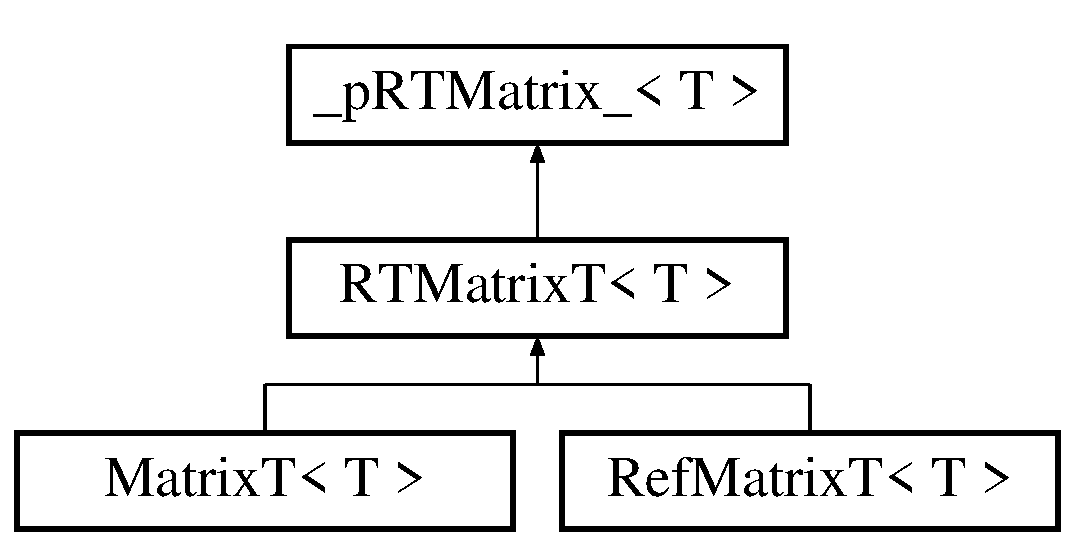
\includegraphics[height=3.000000cm]{class__pRTMatrix__}
\end{center}
\end{figure}
\subsection*{Public Member Functions}
\begin{DoxyCompactItemize}
\item 
T $\ast$ \hyperlink{class__pRTMatrix___a33cb86fe78d486c97b3f86da122e6e12}{Data} () const 
\item 
uint32 \hyperlink{class__pRTMatrix___a96fbea9ed24b21c0dec32e645972d29b}{DataSize} () const 
\end{DoxyCompactItemize}
\subsection*{Public Attributes}
\begin{DoxyCompactItemize}
\item 
uint32 \hyperlink{class__pRTMatrix___aa43a04344c78d8edef929e758e8e5263}{n}
\item 
uint32 \hyperlink{class__pRTMatrix___a365982f4a3d0d921a124ac0c21b63f6c}{m}
\item 
\hypertarget{class__pRTMatrix___ad12833157985dc5c8331fab12896f00e}{
T $\ast$ {\bfseries data}}
\label{class__pRTMatrix___ad12833157985dc5c8331fab12896f00e}

\item 
\hypertarget{class__pRTMatrix___a985951c3437d2191e9832f77fb544106}{
T $\ast$$\ast$ {\bfseries row}}
\label{class__pRTMatrix___a985951c3437d2191e9832f77fb544106}

\end{DoxyCompactItemize}


\subsection{Detailed Description}
\subsubsection*{template$<$class T$>$class \_\-pRTMatrix\_\-$<$ T $>$}

a Matrix with faster access because of lack of checks 

\subsection{Member Function Documentation}
\hypertarget{class__pRTMatrix___a33cb86fe78d486c97b3f86da122e6e12}{
\index{\_\-pRTMatrix\_\-@{\_\-pRTMatrix\_\-}!Data@{Data}}
\index{Data@{Data}!_pRTMatrix_@{\_\-pRTMatrix\_\-}}
\subsubsection[{Data}]{\setlength{\rightskip}{0pt plus 5cm}template$<$class T$>$ T$\ast$ {\bf \_\-pRTMatrix\_\-}$<$ T $>$::Data (
\begin{DoxyParamCaption}
{}
\end{DoxyParamCaption}
) const\hspace{0.3cm}{\ttfamily  \mbox{[}inline\mbox{]}}}}
\label{class__pRTMatrix___a33cb86fe78d486c97b3f86da122e6e12}
Allow fast access to the packed element structure \hypertarget{class__pRTMatrix___a96fbea9ed24b21c0dec32e645972d29b}{
\index{\_\-pRTMatrix\_\-@{\_\-pRTMatrix\_\-}!DataSize@{DataSize}}
\index{DataSize@{DataSize}!_pRTMatrix_@{\_\-pRTMatrix\_\-}}
\subsubsection[{DataSize}]{\setlength{\rightskip}{0pt plus 5cm}template$<$class T$>$ uint32 {\bf \_\-pRTMatrix\_\-}$<$ T $>$::DataSize (
\begin{DoxyParamCaption}
{}
\end{DoxyParamCaption}
) const\hspace{0.3cm}{\ttfamily  \mbox{[}inline\mbox{]}}}}
\label{class__pRTMatrix___a96fbea9ed24b21c0dec32e645972d29b}
The size as number of MatrixType of the matrix ! It semms to me that const is not useful here, parameter returned by value! by Anton 

\subsection{Member Data Documentation}
\hypertarget{class__pRTMatrix___a365982f4a3d0d921a124ac0c21b63f6c}{
\index{\_\-pRTMatrix\_\-@{\_\-pRTMatrix\_\-}!m@{m}}
\index{m@{m}!_pRTMatrix_@{\_\-pRTMatrix\_\-}}
\subsubsection[{m}]{\setlength{\rightskip}{0pt plus 5cm}template$<$class T$>$ uint32 {\bf \_\-pRTMatrix\_\-}$<$ T $>$::{\bf m}}}
\label{class__pRTMatrix___a365982f4a3d0d921a124ac0c21b63f6c}
n of columns \hypertarget{class__pRTMatrix___aa43a04344c78d8edef929e758e8e5263}{
\index{\_\-pRTMatrix\_\-@{\_\-pRTMatrix\_\-}!n@{n}}
\index{n@{n}!_pRTMatrix_@{\_\-pRTMatrix\_\-}}
\subsubsection[{n}]{\setlength{\rightskip}{0pt plus 5cm}template$<$class T$>$ uint32 {\bf \_\-pRTMatrix\_\-}$<$ T $>$::{\bf n}}}
\label{class__pRTMatrix___aa43a04344c78d8edef929e758e8e5263}
n of rows 

The documentation for this class was generated from the following file:\begin{DoxyCompactItemize}
\item 
\hyperlink{RTMatrix_8h}{RTMatrix.h}\end{DoxyCompactItemize}

\hypertarget{classCDBBrowserMenu}{
\section{CDBBrowserMenu Class Reference}
\label{classCDBBrowserMenu}\index{CDBBrowserMenu@{CDBBrowserMenu}}
}


{\ttfamily \#include $<$CDBBrowserMenu.h$>$}

\subsection*{Public Member Functions}
\begin{DoxyCompactItemize}
\item 
virtual const char $\ast$ \hyperlink{classCDBBrowserMenu_a60b762702881e68c3e8e24cf6d2f8aa8}{Title} ()
\item 
\hypertarget{classCDBBrowserMenu_abdbb85ea44d7b6f93db922311a6401a3}{
virtual void {\bfseries SetTitle} (const char $\ast$\hyperlink{classCDBBrowserMenu_a398c0c3251532f4b924001c2b4fe3427}{title})}
\label{classCDBBrowserMenu_abdbb85ea44d7b6f93db922311a6401a3}

\item 
\hyperlink{classCDBBrowserMenu_abc789c1da32237b02438a1555e4f1e0b}{CDBBrowserMenu} ()
\item 
\hyperlink{classCDBBrowserMenu_a1b3621101f19a48ef37c213b0751393c}{$\sim$CDBBrowserMenu} ()
\item 
bool \hyperlink{classCDBBrowserMenu_aa81bfa7140426c04ce743cbe0a0f8bf5}{LinkTo} (const char $\ast$cdbName, ConfigurationDataBase \&cdb)
\item 
virtual bool \hyperlink{classCDBBrowserMenu_a9c5c708189ef3f7cc9d5131a0e38006e}{TextMenu} (StreamInterface \&in, StreamInterface \&out)
\item 
virtual bool \hyperlink{classCDBBrowserMenu_a8c8b793d08fd4e836fd8f9f54faf1e8e}{ObjectSaveSetup} (ConfigurationDataBase \&info, StreamInterface $\ast$err)
\item 
virtual bool \hyperlink{classCDBBrowserMenu_a7284f261814bba2876c344495ff89475}{ObjectLoadSetup} (ConfigurationDataBase \&info, StreamInterface $\ast$err)
\end{DoxyCompactItemize}
\subsection*{Protected Member Functions}
\begin{DoxyCompactItemize}
\item 
virtual bool \hyperlink{classCDBBrowserMenu_a70984d895ae73fb90e3886cd6467bd8c}{ProcessHttpMessage} (HttpStream \&hStream)
\end{DoxyCompactItemize}
\subsection*{Protected Attributes}
\begin{DoxyCompactItemize}
\item 
BString \hyperlink{classCDBBrowserMenu_a398c0c3251532f4b924001c2b4fe3427}{title}
\end{DoxyCompactItemize}
\subsection*{Friends}
\begin{DoxyCompactItemize}
\item 
bool \hyperlink{classCDBBrowserMenu_a0f2e4df78baa29b840ff920877e3a35b}{CDB2Setup} (\hyperlink{classCDBBrowserMenu}{CDBBrowserMenu} \&cdbBrowse, const char $\ast$cdbName, ConfigurationDataBase \&cdbRef)
\end{DoxyCompactItemize}


\subsection{Detailed Description}
allows browsing a CDB via the MenuSystem 

\subsection{Constructor \& Destructor Documentation}
\hypertarget{classCDBBrowserMenu_abc789c1da32237b02438a1555e4f1e0b}{
\index{CDBBrowserMenu@{CDBBrowserMenu}!CDBBrowserMenu@{CDBBrowserMenu}}
\index{CDBBrowserMenu@{CDBBrowserMenu}!CDBBrowserMenu@{CDBBrowserMenu}}
\subsubsection[{CDBBrowserMenu}]{\setlength{\rightskip}{0pt plus 5cm}CDBBrowserMenu::CDBBrowserMenu (
\begin{DoxyParamCaption}
{}
\end{DoxyParamCaption}
)\hspace{0.3cm}{\ttfamily  \mbox{[}inline\mbox{]}}}}
\label{classCDBBrowserMenu_abc789c1da32237b02438a1555e4f1e0b}
\hypertarget{classCDBBrowserMenu_a1b3621101f19a48ef37c213b0751393c}{
\index{CDBBrowserMenu@{CDBBrowserMenu}!$\sim$CDBBrowserMenu@{$\sim$CDBBrowserMenu}}
\index{$\sim$CDBBrowserMenu@{$\sim$CDBBrowserMenu}!CDBBrowserMenu@{CDBBrowserMenu}}
\subsubsection[{$\sim$CDBBrowserMenu}]{\setlength{\rightskip}{0pt plus 5cm}CDBBrowserMenu::$\sim$CDBBrowserMenu (
\begin{DoxyParamCaption}
{}
\end{DoxyParamCaption}
)\hspace{0.3cm}{\ttfamily  \mbox{[}inline\mbox{]}}}}
\label{classCDBBrowserMenu_a1b3621101f19a48ef37c213b0751393c}


\subsection{Member Function Documentation}
\hypertarget{classCDBBrowserMenu_aa81bfa7140426c04ce743cbe0a0f8bf5}{
\index{CDBBrowserMenu@{CDBBrowserMenu}!LinkTo@{LinkTo}}
\index{LinkTo@{LinkTo}!CDBBrowserMenu@{CDBBrowserMenu}}
\subsubsection[{LinkTo}]{\setlength{\rightskip}{0pt plus 5cm}bool CDBBrowserMenu::LinkTo (
\begin{DoxyParamCaption}
\item[{const char $\ast$}]{cdbName, }
\item[{ConfigurationDataBase \&}]{cdb}
\end{DoxyParamCaption}
)\hspace{0.3cm}{\ttfamily  \mbox{[}inline\mbox{]}}}}
\label{classCDBBrowserMenu_aa81bfa7140426c04ce743cbe0a0f8bf5}
Sets the database to browse \hypertarget{classCDBBrowserMenu_a7284f261814bba2876c344495ff89475}{
\index{CDBBrowserMenu@{CDBBrowserMenu}!ObjectLoadSetup@{ObjectLoadSetup}}
\index{ObjectLoadSetup@{ObjectLoadSetup}!CDBBrowserMenu@{CDBBrowserMenu}}
\subsubsection[{ObjectLoadSetup}]{\setlength{\rightskip}{0pt plus 5cm}virtual bool CDBBrowserMenu::ObjectLoadSetup (
\begin{DoxyParamCaption}
\item[{ConfigurationDataBase \&}]{info, }
\item[{StreamInterface $\ast$}]{err}
\end{DoxyParamCaption}
)\hspace{0.3cm}{\ttfamily  \mbox{[}inline, virtual\mbox{]}}}}
\label{classCDBBrowserMenu_a7284f261814bba2876c344495ff89475}
initialise an object from a set of configs \hypertarget{classCDBBrowserMenu_a8c8b793d08fd4e836fd8f9f54faf1e8e}{
\index{CDBBrowserMenu@{CDBBrowserMenu}!ObjectSaveSetup@{ObjectSaveSetup}}
\index{ObjectSaveSetup@{ObjectSaveSetup}!CDBBrowserMenu@{CDBBrowserMenu}}
\subsubsection[{ObjectSaveSetup}]{\setlength{\rightskip}{0pt plus 5cm}virtual bool CDBBrowserMenu::ObjectSaveSetup (
\begin{DoxyParamCaption}
\item[{ConfigurationDataBase \&}]{info, }
\item[{StreamInterface $\ast$}]{err}
\end{DoxyParamCaption}
)\hspace{0.3cm}{\ttfamily  \mbox{[}inline, virtual\mbox{]}}}}
\label{classCDBBrowserMenu_a8c8b793d08fd4e836fd8f9f54faf1e8e}
save an object content into a set of configs \hypertarget{classCDBBrowserMenu_a70984d895ae73fb90e3886cd6467bd8c}{
\index{CDBBrowserMenu@{CDBBrowserMenu}!ProcessHttpMessage@{ProcessHttpMessage}}
\index{ProcessHttpMessage@{ProcessHttpMessage}!CDBBrowserMenu@{CDBBrowserMenu}}
\subsubsection[{ProcessHttpMessage}]{\setlength{\rightskip}{0pt plus 5cm}virtual bool CDBBrowserMenu::ProcessHttpMessage (
\begin{DoxyParamCaption}
\item[{HttpStream \&}]{hStream}
\end{DoxyParamCaption}
)\hspace{0.3cm}{\ttfamily  \mbox{[}inline, protected, virtual\mbox{]}}}}
\label{classCDBBrowserMenu_a70984d895ae73fb90e3886cd6467bd8c}
The HTTP entry point \hypertarget{classCDBBrowserMenu_a9c5c708189ef3f7cc9d5131a0e38006e}{
\index{CDBBrowserMenu@{CDBBrowserMenu}!TextMenu@{TextMenu}}
\index{TextMenu@{TextMenu}!CDBBrowserMenu@{CDBBrowserMenu}}
\subsubsection[{TextMenu}]{\setlength{\rightskip}{0pt plus 5cm}virtual bool CDBBrowserMenu::TextMenu (
\begin{DoxyParamCaption}
\item[{StreamInterface \&}]{in, }
\item[{StreamInterface \&}]{out}
\end{DoxyParamCaption}
)\hspace{0.3cm}{\ttfamily  \mbox{[}inline, virtual\mbox{]}}}}
\label{classCDBBrowserMenu_a9c5c708189ef3f7cc9d5131a0e38006e}
\hypertarget{classCDBBrowserMenu_a60b762702881e68c3e8e24cf6d2f8aa8}{
\index{CDBBrowserMenu@{CDBBrowserMenu}!Title@{Title}}
\index{Title@{Title}!CDBBrowserMenu@{CDBBrowserMenu}}
\subsubsection[{Title}]{\setlength{\rightskip}{0pt plus 5cm}virtual const char$\ast$ CDBBrowserMenu::Title (
\begin{DoxyParamCaption}
{}
\end{DoxyParamCaption}
)\hspace{0.3cm}{\ttfamily  \mbox{[}inline, virtual\mbox{]}}}}
\label{classCDBBrowserMenu_a60b762702881e68c3e8e24cf6d2f8aa8}
to be able to choose the labelling policy 

\subsection{Friends And Related Function Documentation}
\hypertarget{classCDBBrowserMenu_a0f2e4df78baa29b840ff920877e3a35b}{
\index{CDBBrowserMenu@{CDBBrowserMenu}!CDB2Setup@{CDB2Setup}}
\index{CDB2Setup@{CDB2Setup}!CDBBrowserMenu@{CDBBrowserMenu}}
\subsubsection[{CDB2Setup}]{\setlength{\rightskip}{0pt plus 5cm}bool CDB2Setup (
\begin{DoxyParamCaption}
\item[{{\bf CDBBrowserMenu} \&}]{cdbBrowse, }
\item[{const char $\ast$}]{cdbName, }
\item[{ConfigurationDataBase \&}]{cdbRef}
\end{DoxyParamCaption}
)\hspace{0.3cm}{\ttfamily  \mbox{[}friend\mbox{]}}}}
\label{classCDBBrowserMenu_a0f2e4df78baa29b840ff920877e3a35b}


\subsection{Member Data Documentation}
\hypertarget{classCDBBrowserMenu_a398c0c3251532f4b924001c2b4fe3427}{
\index{CDBBrowserMenu@{CDBBrowserMenu}!title@{title}}
\index{title@{title}!CDBBrowserMenu@{CDBBrowserMenu}}
\subsubsection[{title}]{\setlength{\rightskip}{0pt plus 5cm}BString {\bf CDBBrowserMenu::title}\hspace{0.3cm}{\ttfamily  \mbox{[}protected\mbox{]}}}}
\label{classCDBBrowserMenu_a398c0c3251532f4b924001c2b4fe3427}
a specific title, distinct from the object name 

The documentation for this class was generated from the following file:\begin{DoxyCompactItemize}
\item 
\hyperlink{CDBBrowserMenu_8h}{CDBBrowserMenu.h}\end{DoxyCompactItemize}

\hypertarget{classColormapInterface}{
\section{ColormapInterface Class Reference}
\label{classColormapInterface}\index{ColormapInterface@{ColormapInterface}}
}
Inheritance diagram for ColormapInterface:\begin{figure}[H]
\begin{center}
\leavevmode
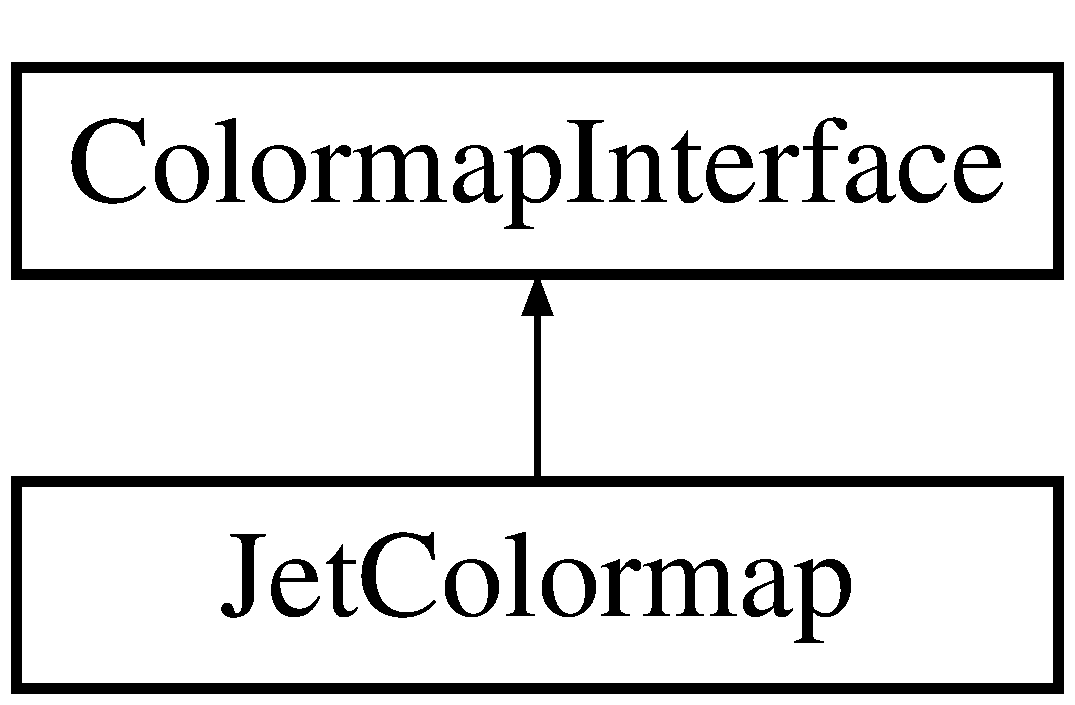
\includegraphics[height=2.000000cm]{classColormapInterface}
\end{center}
\end{figure}
\subsection*{Public Member Functions}
\begin{DoxyCompactItemize}
\item 
\hypertarget{classColormapInterface_a88621931bd86e21b18c9fb8901e52de2}{
\hyperlink{classColormapInterface_a88621931bd86e21b18c9fb8901e52de2}{ColormapInterface} ()}
\label{classColormapInterface_a88621931bd86e21b18c9fb8901e52de2}

\begin{DoxyCompactList}\small\item\em Default constructor. \end{DoxyCompactList}\item 
\hypertarget{classColormapInterface_abbaf26c369c77b8ce2f34e5f6e23e448}{
\hyperlink{classColormapInterface_abbaf26c369c77b8ce2f34e5f6e23e448}{ColormapInterface} (int32 numberOfColors)}
\label{classColormapInterface_abbaf26c369c77b8ce2f34e5f6e23e448}

\begin{DoxyCompactList}\small\item\em Alternative constructor. \end{DoxyCompactList}\item 
\hypertarget{classColormapInterface_ad21f99624caa4f23ca91c618424212f6}{
\hyperlink{classColormapInterface_ad21f99624caa4f23ca91c618424212f6}{$\sim$ColormapInterface} ()}
\label{classColormapInterface_ad21f99624caa4f23ca91c618424212f6}

\begin{DoxyCompactList}\small\item\em Destructor. \end{DoxyCompactList}\item 
\hypertarget{classColormapInterface_a292f9e7d4527205058dbf518783237f6}{
bool \hyperlink{classColormapInterface_a292f9e7d4527205058dbf518783237f6}{SetSize} (int32 numberOfColors)}
\label{classColormapInterface_a292f9e7d4527205058dbf518783237f6}

\begin{DoxyCompactList}\small\item\em Set number of colors in colormap (color table) \end{DoxyCompactList}\item 
\hypertarget{classColormapInterface_a568a705be78926a1c8cc1b459280341b}{
void {\bfseries SetStartValue} (float startValue)}
\label{classColormapInterface_a568a705be78926a1c8cc1b459280341b}

\item 
\hypertarget{classColormapInterface_a881042c149d035141b8a6a665fa23118}{
void {\bfseries SetEndValue} (float endValue)}
\label{classColormapInterface_a881042c149d035141b8a6a665fa23118}

\item 
\hypertarget{classColormapInterface_aee7a172a11995765c9ac099769b4616b}{
\hyperlink{structsColormap}{sColormap} $\ast$ {\bfseries CMap} ()}
\label{classColormapInterface_aee7a172a11995765c9ac099769b4616b}

\item 
\hypertarget{classColormapInterface_a6d7bce43dd54507ad5afeb08893d882e}{
int32 {\bfseries NColors} ()}
\label{classColormapInterface_a6d7bce43dd54507ad5afeb08893d882e}

\item 
\hypertarget{classColormapInterface_a3ff1b9f35c8100cf5eb371a5ccb226b4}{
float {\bfseries StartValue} ()}
\label{classColormapInterface_a3ff1b9f35c8100cf5eb371a5ccb226b4}

\item 
\hypertarget{classColormapInterface_a6a154f895822ddf3b8b3dfcb60ee3650}{
float {\bfseries EndValue} ()}
\label{classColormapInterface_a6a154f895822ddf3b8b3dfcb60ee3650}

\item 
\hypertarget{classColormapInterface_ac004257f5873631c251a07a73751642a}{
bool {\bfseries GetColorCode} (float value, \hyperlink{structsColormap}{sColormap} $\ast$color)}
\label{classColormapInterface_ac004257f5873631c251a07a73751642a}

\end{DoxyCompactItemize}
\subsection*{Protected Member Functions}
\begin{DoxyCompactItemize}
\item 
\hypertarget{classColormapInterface_a6a21ed77cc32412d0888843ab5a72ab5}{
virtual bool {\bfseries BuildJetColorMap} ()=0}
\label{classColormapInterface_a6a21ed77cc32412d0888843ab5a72ab5}

\end{DoxyCompactItemize}
\subsection*{Protected Attributes}
\begin{DoxyCompactItemize}
\item 
\hypertarget{classColormapInterface_a53e082b9c531202c5a2c16ab8756cd12}{
int32 {\bfseries nColors}}
\label{classColormapInterface_a53e082b9c531202c5a2c16ab8756cd12}

\item 
\hypertarget{classColormapInterface_a8296ac6513e88ddfb8b33fbb64cf4a8f}{
\hyperlink{structsColormap}{sColormap} $\ast$ {\bfseries cMap}}
\label{classColormapInterface_a8296ac6513e88ddfb8b33fbb64cf4a8f}

\item 
\hypertarget{classColormapInterface_af09c625b10de3076dccfc8723a36c59a}{
float {\bfseries startVal}}
\label{classColormapInterface_af09c625b10de3076dccfc8723a36c59a}

\item 
\hypertarget{classColormapInterface_a55bb9c728c3629125ef9fbd5ed2d7d5a}{
float {\bfseries endVal}}
\label{classColormapInterface_a55bb9c728c3629125ef9fbd5ed2d7d5a}

\end{DoxyCompactItemize}


The documentation for this class was generated from the following file:\begin{DoxyCompactItemize}
\item 
\hyperlink{ColormapInterface_8h}{ColormapInterface.h}\end{DoxyCompactItemize}

\hypertarget{classConstantWaveform}{
\section{ConstantWaveform Class Reference}
\label{classConstantWaveform}\index{ConstantWaveform@{ConstantWaveform}}
}
Inheritance diagram for ConstantWaveform:\begin{figure}[H]
\begin{center}
\leavevmode
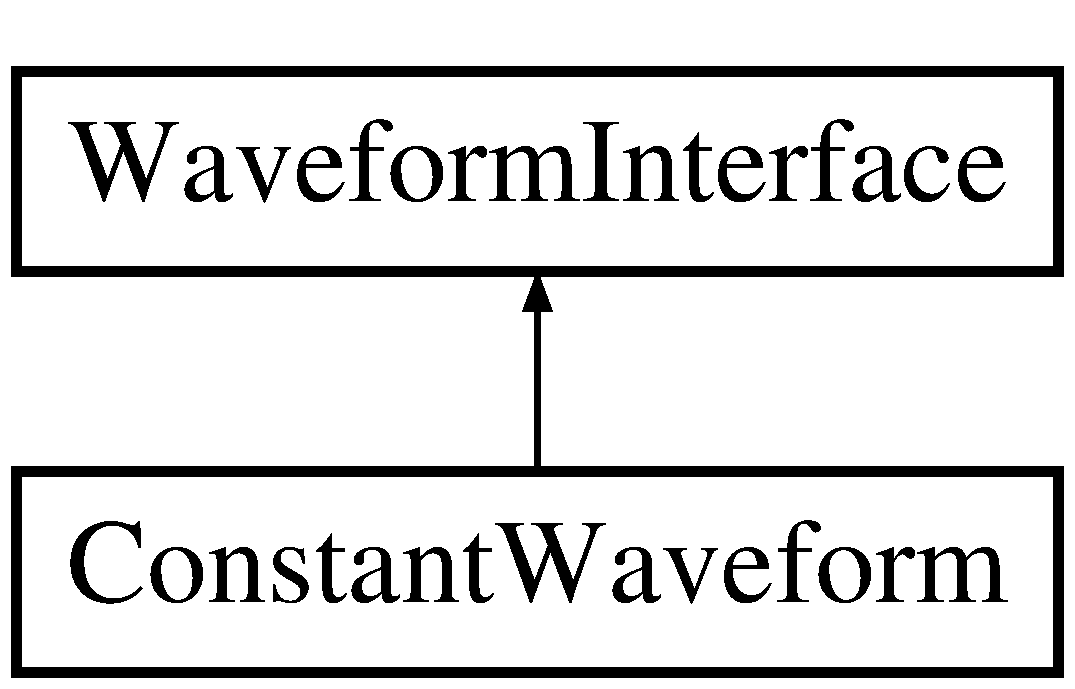
\includegraphics[height=2.000000cm]{classConstantWaveform}
\end{center}
\end{figure}
\subsection*{Public Member Functions}
\begin{DoxyCompactItemize}
\item 
\hypertarget{classConstantWaveform_a166066a7ab0b916babf93204028960b2}{
virtual void {\bfseries Reset} ()}
\label{classConstantWaveform_a166066a7ab0b916babf93204028960b2}

\item 
\hypertarget{classConstantWaveform_abc4f775c3b201a12e679b7a190820bfb}{
virtual bool {\bfseries ObjectLoadSetup} (ConfigurationDataBase \&cdbData, StreamInterface $\ast$err)}
\label{classConstantWaveform_abc4f775c3b201a12e679b7a190820bfb}

\item 
\hypertarget{classConstantWaveform_a9dcbac26e69bd407cff94e7cbd32cc39}{
virtual bool {\bfseries ProcessHttpMessage} (HttpStream \&hStream)}
\label{classConstantWaveform_a9dcbac26e69bd407cff94e7cbd32cc39}

\item 
\hypertarget{classConstantWaveform_a05df91e7d445cc903f950f40b4915ba4}{
virtual float {\bfseries GetValue} (int32 usecTime)}
\label{classConstantWaveform_a05df91e7d445cc903f950f40b4915ba4}

\end{DoxyCompactItemize}


The documentation for this class was generated from the following files:\begin{DoxyCompactItemize}
\item 
\hyperlink{ConstantWaveform_8h}{ConstantWaveform.h}\item 
ConstantWaveform.cpp\end{DoxyCompactItemize}

\hypertarget{structCoord2D}{
\section{Coord2D Struct Reference}
\label{structCoord2D}\index{Coord2D@{Coord2D}}
}


{\ttfamily \#include $<$poloidalCoord.h$>$}

\subsection*{Public Attributes}
\begin{DoxyCompactItemize}
\item 
\hypertarget{structCoord2D_ace9c2672c56fe87ebe224cb30c536d5a}{
float {\bfseries R}}
\label{structCoord2D_ace9c2672c56fe87ebe224cb30c536d5a}

\item 
\hypertarget{structCoord2D_a74f3264d4c18705c1b1d39995d053971}{
float {\bfseries Z}}
\label{structCoord2D_a74f3264d4c18705c1b1d39995d053971}

\end{DoxyCompactItemize}


\subsection{Detailed Description}
a simple type that can be staically initialized 

The documentation for this struct was generated from the following file:\begin{DoxyCompactItemize}
\item 
\hyperlink{poloidalCoord_8h}{poloidalCoord.h}\end{DoxyCompactItemize}

\hypertarget{classDirectoryMenuBrowser}{
\section{DirectoryMenuBrowser Class Reference}
\label{classDirectoryMenuBrowser}\index{DirectoryMenuBrowser@{DirectoryMenuBrowser}}
}
\subsection*{Public Member Functions}
\begin{DoxyCompactItemize}
\item 
void \hyperlink{classDirectoryMenuBrowser_a5bdd2f9fb925790dd4e08617b60d066d}{SetUp} (MenuSystemAction $\ast$action, void $\ast$userData, const char $\ast$path=\char`\"{}.\char`\"{})
\item 
virtual bool \hyperlink{classDirectoryMenuBrowser_a9c0b2bb9b511a604ba38c615045c9f15}{TextMenu} (StreamInterface \&in, StreamInterface \&out)
\item 
\hypertarget{classDirectoryMenuBrowser_a0da24dcaedb5fe75a11fa61f4018b4c3}{
virtual bool {\bfseries ProcessHttpMessage} (HttpStream \&hStream)}
\label{classDirectoryMenuBrowser_a0da24dcaedb5fe75a11fa61f4018b4c3}

\end{DoxyCompactItemize}
\subsection*{Friends}
\begin{DoxyCompactItemize}
\item 
\hypertarget{classDirectoryMenuBrowser_ac9fad7372844b75a86dfa4667fc05740}{
bool {\bfseries DIRMenuSystemTextMenu} (\hyperlink{classDirectoryMenuBrowser}{DirectoryMenuBrowser} \&dir, StreamInterface \&in, StreamInterface \&out)}
\label{classDirectoryMenuBrowser_ac9fad7372844b75a86dfa4667fc05740}

\item 
\hypertarget{classDirectoryMenuBrowser_abd80802f2f38a2fa5362a8567979bc9e}{
bool {\bfseries DIRUserDefinedAction} (StreamInterface \&in, StreamInterface \&out, void $\ast$dir)}
\label{classDirectoryMenuBrowser_abd80802f2f38a2fa5362a8567979bc9e}

\item 
bool \hyperlink{classDirectoryMenuBrowser_aedce0dcf59ae7a4a7d32f2696e86ba11}{DIRMProcessHttpMessage} (\hyperlink{classDirectoryMenuBrowser}{DirectoryMenuBrowser} \&dir, HttpStream \&hStream)
\end{DoxyCompactItemize}


\subsection{Member Function Documentation}
\hypertarget{classDirectoryMenuBrowser_a5bdd2f9fb925790dd4e08617b60d066d}{
\index{DirectoryMenuBrowser@{DirectoryMenuBrowser}!SetUp@{SetUp}}
\index{SetUp@{SetUp}!DirectoryMenuBrowser@{DirectoryMenuBrowser}}
\subsubsection[{SetUp}]{\setlength{\rightskip}{0pt plus 5cm}void DirectoryMenuBrowser::SetUp (
\begin{DoxyParamCaption}
\item[{MenuSystemAction $\ast$}]{action, }
\item[{void $\ast$}]{userData, }
\item[{const char $\ast$}]{path = {\ttfamily \char`\"{}.\char`\"{}}}
\end{DoxyParamCaption}
)\hspace{0.3cm}{\ttfamily  \mbox{[}inline\mbox{]}}}}
\label{classDirectoryMenuBrowser_a5bdd2f9fb925790dd4e08617b60d066d}
Sets the action associated with this menu item \hypertarget{classDirectoryMenuBrowser_a9c0b2bb9b511a604ba38c615045c9f15}{
\index{DirectoryMenuBrowser@{DirectoryMenuBrowser}!TextMenu@{TextMenu}}
\index{TextMenu@{TextMenu}!DirectoryMenuBrowser@{DirectoryMenuBrowser}}
\subsubsection[{TextMenu}]{\setlength{\rightskip}{0pt plus 5cm}virtual bool DirectoryMenuBrowser::TextMenu (
\begin{DoxyParamCaption}
\item[{StreamInterface \&}]{in, }
\item[{StreamInterface \&}]{out}
\end{DoxyParamCaption}
)\hspace{0.3cm}{\ttfamily  \mbox{[}inline, virtual\mbox{]}}}}
\label{classDirectoryMenuBrowser_a9c0b2bb9b511a604ba38c615045c9f15}
to call the menu 

\subsection{Friends And Related Function Documentation}
\hypertarget{classDirectoryMenuBrowser_aedce0dcf59ae7a4a7d32f2696e86ba11}{
\index{DirectoryMenuBrowser@{DirectoryMenuBrowser}!DIRMProcessHttpMessage@{DIRMProcessHttpMessage}}
\index{DIRMProcessHttpMessage@{DIRMProcessHttpMessage}!DirectoryMenuBrowser@{DirectoryMenuBrowser}}
\subsubsection[{DIRMProcessHttpMessage}]{\setlength{\rightskip}{0pt plus 5cm}bool DIRMProcessHttpMessage (
\begin{DoxyParamCaption}
\item[{{\bf DirectoryMenuBrowser} \&}]{dir, }
\item[{HttpStream \&}]{hStream}
\end{DoxyParamCaption}
)\hspace{0.3cm}{\ttfamily  \mbox{[}friend\mbox{]}}}}
\label{classDirectoryMenuBrowser_aedce0dcf59ae7a4a7d32f2696e86ba11}


LIST ALL THE LINKS FIRST 



The documentation for this class was generated from the following file:\begin{DoxyCompactItemize}
\item 
\hyperlink{DirectoryMenuBrowser_8h}{DirectoryMenuBrowser.h}\end{DoxyCompactItemize}

\hypertarget{classDummyVirtual}{
\section{DummyVirtual Class Reference}
\label{classDummyVirtual}\index{DummyVirtual@{DummyVirtual}}
}
\subsection*{Public Member Functions}
\begin{DoxyCompactItemize}
\item 
virtual \hyperlink{classDummyVirtual_ab4d0bdbb8d26b4d06e9d6feba243ee45}{$\sim$DummyVirtual} ()
\end{DoxyCompactItemize}


\subsection{Detailed Description}
a class with a virtual table! 

\subsection{Constructor \& Destructor Documentation}
\hypertarget{classDummyVirtual_ab4d0bdbb8d26b4d06e9d6feba243ee45}{
\index{DummyVirtual@{DummyVirtual}!$\sim$DummyVirtual@{$\sim$DummyVirtual}}
\index{$\sim$DummyVirtual@{$\sim$DummyVirtual}!DummyVirtual@{DummyVirtual}}
\subsubsection[{$\sim$DummyVirtual}]{\setlength{\rightskip}{0pt plus 5cm}virtual DummyVirtual::$\sim$DummyVirtual (
\begin{DoxyParamCaption}
{}
\end{DoxyParamCaption}
)\hspace{0.3cm}{\ttfamily  \mbox{[}inline, virtual\mbox{]}}}}
\label{classDummyVirtual_ab4d0bdbb8d26b4d06e9d6feba243ee45}


The documentation for this class was generated from the following file:\begin{DoxyCompactItemize}
\item 
MMCDBItem.cpp\end{DoxyCompactItemize}

\hypertarget{classExceptionInformation}{
\section{ExceptionInformation Class Reference}
\label{classExceptionInformation}\index{ExceptionInformation@{ExceptionInformation}}
}


{\ttfamily \#include $<$ExceptionInformation.h$>$}

\subsection*{Public Member Functions}
\begin{DoxyCompactItemize}
\item 
void \hyperlink{classExceptionInformation_a09a5a71b16f34e238d941d6a25d25cba}{CleanUp} ()
\item 
\hyperlink{classExceptionInformation_a62fd4e80cab8ec8b6b625250ba72aec2}{ExceptionInformation} ()
\end{DoxyCompactItemize}
\subsection*{Static Public Member Functions}
\begin{DoxyCompactItemize}
\item 
static const char $\ast$ \hyperlink{classExceptionInformation_a83fc9443d97f84ae95aa86cebf3fb688}{ExplainExceptionType} (uint32 type)
\end{DoxyCompactItemize}
\subsection*{Public Attributes}
\begin{DoxyCompactItemize}
\item 
uint32 \hyperlink{classExceptionInformation_a00c1f0031b92c644f1713c1b4e8bb195}{exceptionType}
\item 
uint32 \hyperlink{classExceptionInformation_ae0608cd7a56716e60946c10c36ae132a}{exceptionAddress}
\item 
uint32 \hyperlink{classExceptionInformation_a38fb450b3af0d70d1d06776ae9835c84}{exceptionAccessAddress}
\item 
FString \hyperlink{classExceptionInformation_af1203c0eca73957dbeb5c484eacd10df}{infoStr}
\end{DoxyCompactItemize}


\subsection{Detailed Description}
platform specific exception information 

\subsection{Constructor \& Destructor Documentation}
\hypertarget{classExceptionInformation_a62fd4e80cab8ec8b6b625250ba72aec2}{
\index{ExceptionInformation@{ExceptionInformation}!ExceptionInformation@{ExceptionInformation}}
\index{ExceptionInformation@{ExceptionInformation}!ExceptionInformation@{ExceptionInformation}}
\subsubsection[{ExceptionInformation}]{\setlength{\rightskip}{0pt plus 5cm}ExceptionInformation::ExceptionInformation (
\begin{DoxyParamCaption}
{}
\end{DoxyParamCaption}
)\hspace{0.3cm}{\ttfamily  \mbox{[}inline\mbox{]}}}}
\label{classExceptionInformation_a62fd4e80cab8ec8b6b625250ba72aec2}


\subsection{Member Function Documentation}
\hypertarget{classExceptionInformation_a09a5a71b16f34e238d941d6a25d25cba}{
\index{ExceptionInformation@{ExceptionInformation}!CleanUp@{CleanUp}}
\index{CleanUp@{CleanUp}!ExceptionInformation@{ExceptionInformation}}
\subsubsection[{CleanUp}]{\setlength{\rightskip}{0pt plus 5cm}void ExceptionInformation::CleanUp (
\begin{DoxyParamCaption}
{}
\end{DoxyParamCaption}
)}}
\label{classExceptionInformation_a09a5a71b16f34e238d941d6a25d25cba}
\hypertarget{classExceptionInformation_a83fc9443d97f84ae95aa86cebf3fb688}{
\index{ExceptionInformation@{ExceptionInformation}!ExplainExceptionType@{ExplainExceptionType}}
\index{ExplainExceptionType@{ExplainExceptionType}!ExceptionInformation@{ExceptionInformation}}
\subsubsection[{ExplainExceptionType}]{\setlength{\rightskip}{0pt plus 5cm}const char $\ast$ ExceptionInformation::ExplainExceptionType (
\begin{DoxyParamCaption}
\item[{uint32}]{type}
\end{DoxyParamCaption}
)\hspace{0.3cm}{\ttfamily  \mbox{[}static\mbox{]}}}}
\label{classExceptionInformation_a83fc9443d97f84ae95aa86cebf3fb688}


\subsection{Member Data Documentation}
\hypertarget{classExceptionInformation_a38fb450b3af0d70d1d06776ae9835c84}{
\index{ExceptionInformation@{ExceptionInformation}!exceptionAccessAddress@{exceptionAccessAddress}}
\index{exceptionAccessAddress@{exceptionAccessAddress}!ExceptionInformation@{ExceptionInformation}}
\subsubsection[{exceptionAccessAddress}]{\setlength{\rightskip}{0pt plus 5cm}uint32 {\bf ExceptionInformation::exceptionAccessAddress}}}
\label{classExceptionInformation_a38fb450b3af0d70d1d06776ae9835c84}
where we were trying to access to \hypertarget{classExceptionInformation_ae0608cd7a56716e60946c10c36ae132a}{
\index{ExceptionInformation@{ExceptionInformation}!exceptionAddress@{exceptionAddress}}
\index{exceptionAddress@{exceptionAddress}!ExceptionInformation@{ExceptionInformation}}
\subsubsection[{exceptionAddress}]{\setlength{\rightskip}{0pt plus 5cm}uint32 {\bf ExceptionInformation::exceptionAddress}}}
\label{classExceptionInformation_ae0608cd7a56716e60946c10c36ae132a}
\hypertarget{classExceptionInformation_a00c1f0031b92c644f1713c1b4e8bb195}{
\index{ExceptionInformation@{ExceptionInformation}!exceptionType@{exceptionType}}
\index{exceptionType@{exceptionType}!ExceptionInformation@{ExceptionInformation}}
\subsubsection[{exceptionType}]{\setlength{\rightskip}{0pt plus 5cm}uint32 {\bf ExceptionInformation::exceptionType}}}
\label{classExceptionInformation_a00c1f0031b92c644f1713c1b4e8bb195}
\hypertarget{classExceptionInformation_af1203c0eca73957dbeb5c484eacd10df}{
\index{ExceptionInformation@{ExceptionInformation}!infoStr@{infoStr}}
\index{infoStr@{infoStr}!ExceptionInformation@{ExceptionInformation}}
\subsubsection[{infoStr}]{\setlength{\rightskip}{0pt plus 5cm}FString {\bf ExceptionInformation::infoStr}}}
\label{classExceptionInformation_af1203c0eca73957dbeb5c484eacd10df}


The documentation for this class was generated from the following files:\begin{DoxyCompactItemize}
\item 
\hyperlink{ExceptionInformation_8h}{ExceptionInformation.h}\item 
ExceptionInformation.cpp\end{DoxyCompactItemize}

\hypertarget{classFilter}{
\section{Filter Class Reference}
\label{classFilter}\index{Filter@{Filter}}
}


{\ttfamily \#include $<$Filter.h$>$}

\subsection*{Public Member Functions}
\begin{DoxyCompactItemize}
\item 
\hyperlink{classFilter_a502ee334d42eac3edbaf32b599f9c35e}{$\sim$Filter} ()
\item 
\hyperlink{classFilter_ad15994c30d497afd567a6445446a249e}{Filter} ()
\item 
bool \hyperlink{classFilter_a263b709bcb913eb32cbfd1fc16a2366e}{Init} (ConfigurationDataBase \&cdb)
\item 
void \hyperlink{classFilter_a1c94aa934f9c9af784ff08ea0318f66b}{Reset} (float input=0.0, float output=0.0)
\item 
float \hyperlink{classFilter_a2d6f2a0b780dc773c963b041606c99ab}{Process} (float input)
\end{DoxyCompactItemize}
\subsection*{Friends}
\begin{DoxyCompactItemize}
\item 
bool \hyperlink{classFilter_a228905a165c62822dc1f87333293ba2e}{FilterInit} (\hyperlink{classFilter}{Filter} \&f, ConfigurationDataBase \&cdb)
\item 
bool \hyperlink{classFilter_ab0da466039250753f8c6c878c4f4cdac}{FilterResize} (\hyperlink{classFilter}{Filter} \&f, int inputSize, int outputSize)
\end{DoxyCompactItemize}


\subsection{Detailed Description}
implements a single input single output filter. Initialisation is performed via CDB 

\subsection{Constructor \& Destructor Documentation}
\hypertarget{classFilter_a502ee334d42eac3edbaf32b599f9c35e}{
\index{Filter@{Filter}!$\sim$Filter@{$\sim$Filter}}
\index{$\sim$Filter@{$\sim$Filter}!Filter@{Filter}}
\subsubsection[{$\sim$Filter}]{\setlength{\rightskip}{0pt plus 5cm}Filter::$\sim$Filter (
\begin{DoxyParamCaption}
{}
\end{DoxyParamCaption}
)\hspace{0.3cm}{\ttfamily  \mbox{[}inline\mbox{]}}}}
\label{classFilter_a502ee334d42eac3edbaf32b599f9c35e}
\hypertarget{classFilter_ad15994c30d497afd567a6445446a249e}{
\index{Filter@{Filter}!Filter@{Filter}}
\index{Filter@{Filter}!Filter@{Filter}}
\subsubsection[{Filter}]{\setlength{\rightskip}{0pt plus 5cm}Filter::Filter (
\begin{DoxyParamCaption}
{}
\end{DoxyParamCaption}
)\hspace{0.3cm}{\ttfamily  \mbox{[}inline\mbox{]}}}}
\label{classFilter_ad15994c30d497afd567a6445446a249e}
constructor 

\subsection{Member Function Documentation}
\hypertarget{classFilter_a263b709bcb913eb32cbfd1fc16a2366e}{
\index{Filter@{Filter}!Init@{Init}}
\index{Init@{Init}!Filter@{Filter}}
\subsubsection[{Init}]{\setlength{\rightskip}{0pt plus 5cm}bool Filter::Init (
\begin{DoxyParamCaption}
\item[{ConfigurationDataBase \&}]{cdb}
\end{DoxyParamCaption}
)\hspace{0.3cm}{\ttfamily  \mbox{[}inline\mbox{]}}}}
\label{classFilter_a263b709bcb913eb32cbfd1fc16a2366e}
Numerator = \{a0 a1 a2....\} Denominator= \{b0 b1 ..... \}

OR

0 = \{a0 a1 a2....\} b0 assumed to be 1 1 = \{-\/b1 -\/b2..... \}

OR

Poles = \{p0 p1 ... \} =$>$ p0 p1 which means -\/-\/-\/-\/-\/-\/ $\ast$ -\/-\/-\/-\/-\/-\/ S + p0 S + p1

Zeros = \{z0 z1 ... \} S + z0 S + z1 whic means -\/-\/-\/-\/-\/-\/ $\ast$ -\/-\/-\/-\/-\/-\/ z0 z1 SamplingTime = 1e-\/3

Gain = g which multiplies the whole expression

The conversion uses the following equation between S and Z uses 2 (1-\/Z$^\wedge$-\/1) S = -\/-\/-\/-\/-\/-\/-\/-\/-\/-\/ T (1+Z$^\wedge$-\/1)

The first two filter configuration are already expressed in z domain, The last one is expressed in s domain and the \hyperlink{classFilter}{Filter} class discretizes the transfer function using Tustin. \hypertarget{classFilter_a2d6f2a0b780dc773c963b041606c99ab}{
\index{Filter@{Filter}!Process@{Process}}
\index{Process@{Process}!Filter@{Filter}}
\subsubsection[{Process}]{\setlength{\rightskip}{0pt plus 5cm}float Filter::Process (
\begin{DoxyParamCaption}
\item[{float}]{input}
\end{DoxyParamCaption}
)\hspace{0.3cm}{\ttfamily  \mbox{[}inline\mbox{]}}}}
\label{classFilter_a2d6f2a0b780dc773c963b041606c99ab}
\hypertarget{classFilter_a1c94aa934f9c9af784ff08ea0318f66b}{
\index{Filter@{Filter}!Reset@{Reset}}
\index{Reset@{Reset}!Filter@{Filter}}
\subsubsection[{Reset}]{\setlength{\rightskip}{0pt plus 5cm}void Filter::Reset (
\begin{DoxyParamCaption}
\item[{float}]{input = {\ttfamily 0.0}, }
\item[{float}]{output = {\ttfamily 0.0}}
\end{DoxyParamCaption}
)\hspace{0.3cm}{\ttfamily  \mbox{[}inline\mbox{]}}}}
\label{classFilter_a1c94aa934f9c9af784ff08ea0318f66b}


\subsection{Friends And Related Function Documentation}
\hypertarget{classFilter_a228905a165c62822dc1f87333293ba2e}{
\index{Filter@{Filter}!FilterInit@{FilterInit}}
\index{FilterInit@{FilterInit}!Filter@{Filter}}
\subsubsection[{FilterInit}]{\setlength{\rightskip}{0pt plus 5cm}bool FilterInit (
\begin{DoxyParamCaption}
\item[{{\bf Filter} \&}]{f, }
\item[{ConfigurationDataBase \&}]{cdb}
\end{DoxyParamCaption}
)\hspace{0.3cm}{\ttfamily  \mbox{[}friend\mbox{]}}}}
\label{classFilter_a228905a165c62822dc1f87333293ba2e}
\hypertarget{classFilter_ab0da466039250753f8c6c878c4f4cdac}{
\index{Filter@{Filter}!FilterResize@{FilterResize}}
\index{FilterResize@{FilterResize}!Filter@{Filter}}
\subsubsection[{FilterResize}]{\setlength{\rightskip}{0pt plus 5cm}bool FilterResize (
\begin{DoxyParamCaption}
\item[{{\bf Filter} \&}]{f, }
\item[{int}]{inputSize, }
\item[{int}]{outputSize}
\end{DoxyParamCaption}
)\hspace{0.3cm}{\ttfamily  \mbox{[}friend\mbox{]}}}}
\label{classFilter_ab0da466039250753f8c6c878c4f4cdac}


The documentation for this class was generated from the following files:\begin{DoxyCompactItemize}
\item 
\hyperlink{Filter_8h}{Filter.h}\item 
Filter.cpp\end{DoxyCompactItemize}

\hypertarget{classFlotPlotInterface}{
\section{FlotPlotInterface Class Reference}
\label{classFlotPlotInterface}\index{FlotPlotInterface@{FlotPlotInterface}}
}


Provides web plotting with zoom to BaseLib2 classes.  




{\ttfamily \#include $<$FlotPlotInterface.h$>$}

\subsection*{Public Member Functions}
\begin{DoxyCompactItemize}
\item 
virtual \hyperlink{classFlotPlotInterface_a1abecd17218f3063cea03fc7579d7bdf}{$\sim$FlotPlotInterface} ()
\item 
\hyperlink{classFlotPlotInterface_ae63ae90db79db792b5f9e96d81f0ad05}{FlotPlotInterface} ()
\item 
virtual bool \hyperlink{classFlotPlotInterface_aff4a6245a440da563bc32175646b4dca}{ProcessHttpMessage} (HttpStream \&hStream)
\item 
virtual bool \hyperlink{classFlotPlotInterface_a6eda02b2d2919a2e7e23c594ddee68d2}{GetSignalData} (FString xxSignalName, FString yySignalName, GCRTemplate$<$ SignalInterface $>$ \&xxSignal, GCRTemplate$<$ SignalInterface $>$ \&yySignal)=0
\end{DoxyCompactItemize}


\subsection{Detailed Description}
Provides web plotting with zoom to BaseLib2 classes. 

This class is capable of plotting data using using flot: \href{http://code.google.com/p/flot/}{\tt http://code.google.com/p/flot/} It has to be extended by a signal provider implementing the GetSignalData method

The url arguments are:\par
 SignalList=mandatory comma separated signal names\par
 xxSignal=optional signal name for the xx axis\par
 xxMultiplier=a multiplier for the xx values\par
 yyMultiplier=a multiplier for the yy values\par
 drawLines=true to draw the lines between the points (fast)\par
 drawPoints=true to draw a circle around each point (slow)\par
 Width=optional width of the chart (default 600)\par
 Height=optional height of the chart (default 300)\par
 example:http://localhost:8084/BROWSE/FlotPlot/?SignalList=CYCLETIME,TIMERRELATIVEUSECTIME\&xxSignal=TIME\&xxMultiplier=1e-\/6\&yyMultiplier=1e6\par


It also expects to find the flot scripts in the URL \href{http://.../FLOT_DIR/}{\tt http://.../FLOT\_\-DIR/} 

\subsection{Constructor \& Destructor Documentation}
\hypertarget{classFlotPlotInterface_a1abecd17218f3063cea03fc7579d7bdf}{
\index{FlotPlotInterface@{FlotPlotInterface}!$\sim$FlotPlotInterface@{$\sim$FlotPlotInterface}}
\index{$\sim$FlotPlotInterface@{$\sim$FlotPlotInterface}!FlotPlotInterface@{FlotPlotInterface}}
\subsubsection[{$\sim$FlotPlotInterface}]{\setlength{\rightskip}{0pt plus 5cm}virtual FlotPlotInterface::$\sim$FlotPlotInterface (
\begin{DoxyParamCaption}
{}
\end{DoxyParamCaption}
)\hspace{0.3cm}{\ttfamily  \mbox{[}inline, virtual\mbox{]}}}}
\label{classFlotPlotInterface_a1abecd17218f3063cea03fc7579d7bdf}
\hypertarget{classFlotPlotInterface_ae63ae90db79db792b5f9e96d81f0ad05}{
\index{FlotPlotInterface@{FlotPlotInterface}!FlotPlotInterface@{FlotPlotInterface}}
\index{FlotPlotInterface@{FlotPlotInterface}!FlotPlotInterface@{FlotPlotInterface}}
\subsubsection[{FlotPlotInterface}]{\setlength{\rightskip}{0pt plus 5cm}FlotPlotInterface::FlotPlotInterface (
\begin{DoxyParamCaption}
{}
\end{DoxyParamCaption}
)\hspace{0.3cm}{\ttfamily  \mbox{[}inline\mbox{]}}}}
\label{classFlotPlotInterface_ae63ae90db79db792b5f9e96d81f0ad05}


\subsection{Member Function Documentation}
\hypertarget{classFlotPlotInterface_a6eda02b2d2919a2e7e23c594ddee68d2}{
\index{FlotPlotInterface@{FlotPlotInterface}!GetSignalData@{GetSignalData}}
\index{GetSignalData@{GetSignalData}!FlotPlotInterface@{FlotPlotInterface}}
\subsubsection[{GetSignalData}]{\setlength{\rightskip}{0pt plus 5cm}virtual bool FlotPlotInterface::GetSignalData (
\begin{DoxyParamCaption}
\item[{FString}]{xxSignalName, }
\item[{FString}]{yySignalName, }
\item[{GCRTemplate$<$ SignalInterface $>$ \&}]{xxSignal, }
\item[{GCRTemplate$<$ SignalInterface $>$ \&}]{yySignal}
\end{DoxyParamCaption}
)\hspace{0.3cm}{\ttfamily  \mbox{[}pure virtual\mbox{]}}}}
\label{classFlotPlotInterface_a6eda02b2d2919a2e7e23c594ddee68d2}
Retrieve a signal based on the name 
\begin{DoxyParams}{Parameters}
{\em xxSignalName} & the signal name \\
\hline
{\em yySignalName} & the signal yy data encoded in a SignalInterface \\
\hline
{\em xxSignal} & the signal xx data (usually time) encoded in a SignalInterface \\
\hline
{\em yySignal} & the signal yy data encoded in a SignalInterface \\
\hline
\end{DoxyParams}
\begin{DoxyReturn}{Returns}
True if at least the yySignal data is valid 
\end{DoxyReturn}
\hypertarget{classFlotPlotInterface_aff4a6245a440da563bc32175646b4dca}{
\index{FlotPlotInterface@{FlotPlotInterface}!ProcessHttpMessage@{ProcessHttpMessage}}
\index{ProcessHttpMessage@{ProcessHttpMessage}!FlotPlotInterface@{FlotPlotInterface}}
\subsubsection[{ProcessHttpMessage}]{\setlength{\rightskip}{0pt plus 5cm}bool FlotPlotInterface::ProcessHttpMessage (
\begin{DoxyParamCaption}
\item[{HttpStream \&}]{hStream}
\end{DoxyParamCaption}
)\hspace{0.3cm}{\ttfamily  \mbox{[}virtual\mbox{]}}}}
\label{classFlotPlotInterface_aff4a6245a440da563bc32175646b4dca}
The HTTP entry point 

The documentation for this class was generated from the following files:\begin{DoxyCompactItemize}
\item 
\hyperlink{FlotPlotInterface_8h}{FlotPlotInterface.h}\item 
\hyperlink{FlotPlotInterface_8cpp}{FlotPlotInterface.cpp}\end{DoxyCompactItemize}

\hypertarget{classHttpGCRCBrowser}{
\section{HttpGCRCBrowser Class Reference}
\label{classHttpGCRCBrowser}\index{HttpGCRCBrowser@{HttpGCRCBrowser}}
}


{\ttfamily \#include $<$HttpGCRCBrowser.h$>$}

\subsection*{Public Member Functions}
\begin{DoxyCompactItemize}
\item 
virtual const char $\ast$ \hyperlink{classHttpGCRCBrowser_a7c92191d1e87a9dc6ec09981be496fd1}{Title} ()
\item 
\hypertarget{classHttpGCRCBrowser_aa1aecf3ed830811a3fe6cbc156c07070}{
virtual void {\bfseries SetTitle} (const char $\ast$\hyperlink{classHttpGCRCBrowser_a6c59a7dfbebcc1939a60fe4d379630a7}{title})}
\label{classHttpGCRCBrowser_aa1aecf3ed830811a3fe6cbc156c07070}

\item 
\hyperlink{classHttpGCRCBrowser_a311b5a73c2444740ad635e3563ec202b}{HttpGCRCBrowser} ()
\item 
\hyperlink{classHttpGCRCBrowser_a28ae6e58aa3dbccd438ac827d1f25ec4}{$\sim$HttpGCRCBrowser} ()
\item 
virtual bool \hyperlink{classHttpGCRCBrowser_ab18338af4c81014e455b7b563e8e4a7e}{ObjectSaveSetup} (ConfigurationDataBase \&info, StreamInterface $\ast$err)
\item 
virtual bool \hyperlink{classHttpGCRCBrowser_ad2e25b201c478115c72d2c1529069360}{ObjectLoadSetup} (ConfigurationDataBase \&info, StreamInterface $\ast$err)
\end{DoxyCompactItemize}
\subsection*{Protected Member Functions}
\begin{DoxyCompactItemize}
\item 
virtual bool \hyperlink{classHttpGCRCBrowser_a3f93d5e83175c5ebaf8d8811cbfe1828}{ProcessHttpMessage} (HttpStream \&hStream)
\item 
void \hyperlink{classHttpGCRCBrowser_abca6ebb2d9a86a3c2ef6da34719fbe15}{ObjectSubView} (GCRTemplate$<$ GCReferenceContainer $>$ current, const char $\ast$relativePath, const char $\ast$absolutePath, const char $\ast$selector, int level, StreamInterface \&answer)
\end{DoxyCompactItemize}
\subsection*{Protected Attributes}
\begin{DoxyCompactItemize}
\item 
BString \hyperlink{classHttpGCRCBrowser_a6c59a7dfbebcc1939a60fe4d379630a7}{title}
\end{DoxyCompactItemize}


\subsection{Detailed Description}
allows browsing a CDB via the MenuSystem 

\subsection{Constructor \& Destructor Documentation}
\hypertarget{classHttpGCRCBrowser_a311b5a73c2444740ad635e3563ec202b}{
\index{HttpGCRCBrowser@{HttpGCRCBrowser}!HttpGCRCBrowser@{HttpGCRCBrowser}}
\index{HttpGCRCBrowser@{HttpGCRCBrowser}!HttpGCRCBrowser@{HttpGCRCBrowser}}
\subsubsection[{HttpGCRCBrowser}]{\setlength{\rightskip}{0pt plus 5cm}HttpGCRCBrowser::HttpGCRCBrowser (
\begin{DoxyParamCaption}
{}
\end{DoxyParamCaption}
)\hspace{0.3cm}{\ttfamily  \mbox{[}inline\mbox{]}}}}
\label{classHttpGCRCBrowser_a311b5a73c2444740ad635e3563ec202b}
\hypertarget{classHttpGCRCBrowser_a28ae6e58aa3dbccd438ac827d1f25ec4}{
\index{HttpGCRCBrowser@{HttpGCRCBrowser}!$\sim$HttpGCRCBrowser@{$\sim$HttpGCRCBrowser}}
\index{$\sim$HttpGCRCBrowser@{$\sim$HttpGCRCBrowser}!HttpGCRCBrowser@{HttpGCRCBrowser}}
\subsubsection[{$\sim$HttpGCRCBrowser}]{\setlength{\rightskip}{0pt plus 5cm}HttpGCRCBrowser::$\sim$HttpGCRCBrowser (
\begin{DoxyParamCaption}
{}
\end{DoxyParamCaption}
)\hspace{0.3cm}{\ttfamily  \mbox{[}inline\mbox{]}}}}
\label{classHttpGCRCBrowser_a28ae6e58aa3dbccd438ac827d1f25ec4}


\subsection{Member Function Documentation}
\hypertarget{classHttpGCRCBrowser_ad2e25b201c478115c72d2c1529069360}{
\index{HttpGCRCBrowser@{HttpGCRCBrowser}!ObjectLoadSetup@{ObjectLoadSetup}}
\index{ObjectLoadSetup@{ObjectLoadSetup}!HttpGCRCBrowser@{HttpGCRCBrowser}}
\subsubsection[{ObjectLoadSetup}]{\setlength{\rightskip}{0pt plus 5cm}bool HttpGCRCBrowser::ObjectLoadSetup (
\begin{DoxyParamCaption}
\item[{ConfigurationDataBase \&}]{info, }
\item[{StreamInterface $\ast$}]{err}
\end{DoxyParamCaption}
)\hspace{0.3cm}{\ttfamily  \mbox{[}virtual\mbox{]}}}}
\label{classHttpGCRCBrowser_ad2e25b201c478115c72d2c1529069360}
initialise an object from a set of configs The parameter Root determine the subtree of GODB to broswe. Omitting it means the whole tree RootIsHttpRoot can be set to 1 if Root is the same as that of the Http service. This will mean that security will apply correctly and further browsing will work \hypertarget{classHttpGCRCBrowser_ab18338af4c81014e455b7b563e8e4a7e}{
\index{HttpGCRCBrowser@{HttpGCRCBrowser}!ObjectSaveSetup@{ObjectSaveSetup}}
\index{ObjectSaveSetup@{ObjectSaveSetup}!HttpGCRCBrowser@{HttpGCRCBrowser}}
\subsubsection[{ObjectSaveSetup}]{\setlength{\rightskip}{0pt plus 5cm}virtual bool HttpGCRCBrowser::ObjectSaveSetup (
\begin{DoxyParamCaption}
\item[{ConfigurationDataBase \&}]{info, }
\item[{StreamInterface $\ast$}]{err}
\end{DoxyParamCaption}
)\hspace{0.3cm}{\ttfamily  \mbox{[}inline, virtual\mbox{]}}}}
\label{classHttpGCRCBrowser_ab18338af4c81014e455b7b563e8e4a7e}
save an object content into a set of configs \hypertarget{classHttpGCRCBrowser_abca6ebb2d9a86a3c2ef6da34719fbe15}{
\index{HttpGCRCBrowser@{HttpGCRCBrowser}!ObjectSubView@{ObjectSubView}}
\index{ObjectSubView@{ObjectSubView}!HttpGCRCBrowser@{HttpGCRCBrowser}}
\subsubsection[{ObjectSubView}]{\setlength{\rightskip}{0pt plus 5cm}void HttpGCRCBrowser::ObjectSubView (
\begin{DoxyParamCaption}
\item[{GCRTemplate$<$ GCReferenceContainer $>$}]{current, }
\item[{const char $\ast$}]{relativePath, }
\item[{const char $\ast$}]{absolutePath, }
\item[{const char $\ast$}]{selector, }
\item[{int}]{level, }
\item[{StreamInterface \&}]{answer}
\end{DoxyParamCaption}
)\hspace{0.3cm}{\ttfamily  \mbox{[}protected\mbox{]}}}}
\label{classHttpGCRCBrowser_abca6ebb2d9a86a3c2ef6da34719fbe15}


reference to object own page

reference to CDB page 

\hypertarget{classHttpGCRCBrowser_a3f93d5e83175c5ebaf8d8811cbfe1828}{
\index{HttpGCRCBrowser@{HttpGCRCBrowser}!ProcessHttpMessage@{ProcessHttpMessage}}
\index{ProcessHttpMessage@{ProcessHttpMessage}!HttpGCRCBrowser@{HttpGCRCBrowser}}
\subsubsection[{ProcessHttpMessage}]{\setlength{\rightskip}{0pt plus 5cm}bool HttpGCRCBrowser::ProcessHttpMessage (
\begin{DoxyParamCaption}
\item[{HttpStream \&}]{hStream}
\end{DoxyParamCaption}
)\hspace{0.3cm}{\ttfamily  \mbox{[}protected, virtual\mbox{]}}}}
\label{classHttpGCRCBrowser_a3f93d5e83175c5ebaf8d8811cbfe1828}
The HTTP entry point 

see if a structure view is requested

see if a structure view is requested

see if a structure view is requested

see if a structure view is requested

The pointer to the current position 

\hypertarget{classHttpGCRCBrowser_a7c92191d1e87a9dc6ec09981be496fd1}{
\index{HttpGCRCBrowser@{HttpGCRCBrowser}!Title@{Title}}
\index{Title@{Title}!HttpGCRCBrowser@{HttpGCRCBrowser}}
\subsubsection[{Title}]{\setlength{\rightskip}{0pt plus 5cm}virtual const char$\ast$ HttpGCRCBrowser::Title (
\begin{DoxyParamCaption}
{}
\end{DoxyParamCaption}
)\hspace{0.3cm}{\ttfamily  \mbox{[}inline, virtual\mbox{]}}}}
\label{classHttpGCRCBrowser_a7c92191d1e87a9dc6ec09981be496fd1}
to be able to choose the labelling policy 

\subsection{Member Data Documentation}
\hypertarget{classHttpGCRCBrowser_a6c59a7dfbebcc1939a60fe4d379630a7}{
\index{HttpGCRCBrowser@{HttpGCRCBrowser}!title@{title}}
\index{title@{title}!HttpGCRCBrowser@{HttpGCRCBrowser}}
\subsubsection[{title}]{\setlength{\rightskip}{0pt plus 5cm}BString {\bf HttpGCRCBrowser::title}\hspace{0.3cm}{\ttfamily  \mbox{[}protected\mbox{]}}}}
\label{classHttpGCRCBrowser_a6c59a7dfbebcc1939a60fe4d379630a7}
a specific title, distinct from the object name 

The documentation for this class was generated from the following files:\begin{DoxyCompactItemize}
\item 
\hyperlink{HttpGCRCBrowser_8h}{HttpGCRCBrowser.h}\item 
HttpGCRCBrowser.cpp\end{DoxyCompactItemize}

\hypertarget{classIntegerWaveform}{
\section{IntegerWaveform Class Reference}
\label{classIntegerWaveform}\index{IntegerWaveform@{IntegerWaveform}}
}


{\ttfamily \#include $<$IntegerWaveform.h$>$}

\subsection*{Public Member Functions}
\begin{DoxyCompactItemize}
\item 
\hyperlink{classIntegerWaveform_ac3b34133ae90c80c9ae32051cec2611a}{IntegerWaveform} ()
\item 
virtual \hyperlink{classIntegerWaveform_a929899dea90a14cc1ea676df7336d090}{$\sim$IntegerWaveform} ()
\item 
bool \hyperlink{classIntegerWaveform_afb9674852c2d2040508a375c1c5cc8d6}{ObjectLoadSetup} (ConfigurationDataBase \&cdbData)
\item 
float \hyperlink{classIntegerWaveform_ab236b723a92b8f174c65930671887ae6}{GetValue} (int32 usecTime)
\item 
void \hyperlink{classIntegerWaveform_a15587809f76da953aaaf03264298cf5e}{Reset} ()
\item 
float \hyperlink{classIntegerWaveform_ad6582c22eb5896be14805487706711d0}{Minimum} ()
\item 
float \hyperlink{classIntegerWaveform_ad669c89fd753d72f6aca58af1dde2b78}{Maximum} ()
\end{DoxyCompactItemize}


\subsection{Detailed Description}
A waveform which keeps its internal time in microseconds. Note that all slopes are calculated at the moment of creation (function ObjectLoadSetup), and that the waveform has to be resetted (function Reset) between a pulse and the other. 

\subsection{Constructor \& Destructor Documentation}
\hypertarget{classIntegerWaveform_ac3b34133ae90c80c9ae32051cec2611a}{
\index{IntegerWaveform@{IntegerWaveform}!IntegerWaveform@{IntegerWaveform}}
\index{IntegerWaveform@{IntegerWaveform}!IntegerWaveform@{IntegerWaveform}}
\subsubsection[{IntegerWaveform}]{\setlength{\rightskip}{0pt plus 5cm}IntegerWaveform::IntegerWaveform (
\begin{DoxyParamCaption}
{}
\end{DoxyParamCaption}
)\hspace{0.3cm}{\ttfamily  \mbox{[}inline\mbox{]}}}}
\label{classIntegerWaveform_ac3b34133ae90c80c9ae32051cec2611a}
Constructor \hypertarget{classIntegerWaveform_a929899dea90a14cc1ea676df7336d090}{
\index{IntegerWaveform@{IntegerWaveform}!$\sim$IntegerWaveform@{$\sim$IntegerWaveform}}
\index{$\sim$IntegerWaveform@{$\sim$IntegerWaveform}!IntegerWaveform@{IntegerWaveform}}
\subsubsection[{$\sim$IntegerWaveform}]{\setlength{\rightskip}{0pt plus 5cm}virtual IntegerWaveform::$\sim$IntegerWaveform (
\begin{DoxyParamCaption}
{}
\end{DoxyParamCaption}
)\hspace{0.3cm}{\ttfamily  \mbox{[}inline, virtual\mbox{]}}}}
\label{classIntegerWaveform_a929899dea90a14cc1ea676df7336d090}
Deconstructor 

\subsection{Member Function Documentation}
\hypertarget{classIntegerWaveform_ab236b723a92b8f174c65930671887ae6}{
\index{IntegerWaveform@{IntegerWaveform}!GetValue@{GetValue}}
\index{GetValue@{GetValue}!IntegerWaveform@{IntegerWaveform}}
\subsubsection[{GetValue}]{\setlength{\rightskip}{0pt plus 5cm}float IntegerWaveform::GetValue (
\begin{DoxyParamCaption}
\item[{int32}]{usecTime}
\end{DoxyParamCaption}
)\hspace{0.3cm}{\ttfamily  \mbox{[}inline\mbox{]}}}}
\label{classIntegerWaveform_ab236b723a92b8f174c65930671887ae6}
Returns the value of the waveform at a certain time. 
\begin{DoxyParams}{Parameters}
{\em usecTime} & Time in microseconds. Note that usecTime needs to be crescent: in order to obtain the value of the waveform in the past you must Reset it first. \\
\hline
\end{DoxyParams}
\begin{DoxyReturn}{Returns}
The value of the waveform at the specified time. If usecTime is before or after the start or end time of the waveform, the first or last value is held. 
\end{DoxyReturn}
\hypertarget{classIntegerWaveform_ad669c89fd753d72f6aca58af1dde2b78}{
\index{IntegerWaveform@{IntegerWaveform}!Maximum@{Maximum}}
\index{Maximum@{Maximum}!IntegerWaveform@{IntegerWaveform}}
\subsubsection[{Maximum}]{\setlength{\rightskip}{0pt plus 5cm}float IntegerWaveform::Maximum (
\begin{DoxyParamCaption}
{}
\end{DoxyParamCaption}
)\hspace{0.3cm}{\ttfamily  \mbox{[}inline\mbox{]}}}}
\label{classIntegerWaveform_ad669c89fd753d72f6aca58af1dde2b78}
Returns waveform's maximum value. \hypertarget{classIntegerWaveform_ad6582c22eb5896be14805487706711d0}{
\index{IntegerWaveform@{IntegerWaveform}!Minimum@{Minimum}}
\index{Minimum@{Minimum}!IntegerWaveform@{IntegerWaveform}}
\subsubsection[{Minimum}]{\setlength{\rightskip}{0pt plus 5cm}float IntegerWaveform::Minimum (
\begin{DoxyParamCaption}
{}
\end{DoxyParamCaption}
)\hspace{0.3cm}{\ttfamily  \mbox{[}inline\mbox{]}}}}
\label{classIntegerWaveform_ad6582c22eb5896be14805487706711d0}
Returns waveform's minimum value. \hypertarget{classIntegerWaveform_afb9674852c2d2040508a375c1c5cc8d6}{
\index{IntegerWaveform@{IntegerWaveform}!ObjectLoadSetup@{ObjectLoadSetup}}
\index{ObjectLoadSetup@{ObjectLoadSetup}!IntegerWaveform@{IntegerWaveform}}
\subsubsection[{ObjectLoadSetup}]{\setlength{\rightskip}{0pt plus 5cm}bool IntegerWaveform::ObjectLoadSetup (
\begin{DoxyParamCaption}
\item[{ConfigurationDataBase \&}]{cdbData}
\end{DoxyParamCaption}
)\hspace{0.3cm}{\ttfamily  \mbox{[}inline\mbox{]}}}}
\label{classIntegerWaveform_afb9674852c2d2040508a375c1c5cc8d6}
Loads parameters from a CDB 
\begin{DoxyParams}{Parameters}
{\em cdbData} & the CDB \\
\hline
\end{DoxyParams}
\begin{DoxyReturn}{Returns}
True if the initialisation went ok, False otherwise 
\end{DoxyReturn}
\hypertarget{classIntegerWaveform_a15587809f76da953aaaf03264298cf5e}{
\index{IntegerWaveform@{IntegerWaveform}!Reset@{Reset}}
\index{Reset@{Reset}!IntegerWaveform@{IntegerWaveform}}
\subsubsection[{Reset}]{\setlength{\rightskip}{0pt plus 5cm}void IntegerWaveform::Reset (
\begin{DoxyParamCaption}
{}
\end{DoxyParamCaption}
)\hspace{0.3cm}{\ttfamily  \mbox{[}inline\mbox{]}}}}
\label{classIntegerWaveform_a15587809f76da953aaaf03264298cf5e}
Reset function. Resets the internal states and waveforms. To be called in the PREPULSE phase. 

The documentation for this class was generated from the following file:\begin{DoxyCompactItemize}
\item 
\hyperlink{IntegerWaveform_8h}{IntegerWaveform.h}\end{DoxyCompactItemize}

\hypertarget{structIntegerWaveformData}{
\section{IntegerWaveformData Struct Reference}
\label{structIntegerWaveformData}\index{IntegerWaveformData@{IntegerWaveformData}}
}


{\ttfamily \#include $<$IntegerWaveform.h$>$}

\subsection*{Public Attributes}
\begin{DoxyCompactItemize}
\item 
\hypertarget{structIntegerWaveformData_aeec660fc909b067e46c8b29528729561}{
int32 {\bfseries usecTime}}
\label{structIntegerWaveformData_aeec660fc909b067e46c8b29528729561}

\item 
\hypertarget{structIntegerWaveformData_a5c7b0a92aa8cc11f0415c67ea5737eb0}{
float {\bfseries amplitude}}
\label{structIntegerWaveformData_a5c7b0a92aa8cc11f0415c67ea5737eb0}

\item 
\hypertarget{structIntegerWaveformData_adbf9d041356107a09e25e402097b33b1}{
float {\bfseries slope}}
\label{structIntegerWaveformData_adbf9d041356107a09e25e402097b33b1}

\end{DoxyCompactItemize}


\subsection{Detailed Description}
Structure holding data for a single element in an \hyperlink{classIntegerWaveform}{IntegerWaveform}. 

The documentation for this struct was generated from the following file:\begin{DoxyCompactItemize}
\item 
\hyperlink{IntegerWaveform_8h}{IntegerWaveform.h}\end{DoxyCompactItemize}

\hypertarget{classIntegralWaveform}{
\section{IntegralWaveform Class Reference}
\label{classIntegralWaveform}\index{IntegralWaveform@{IntegralWaveform}}
}
Inheritance diagram for IntegralWaveform:\begin{figure}[H]
\begin{center}
\leavevmode
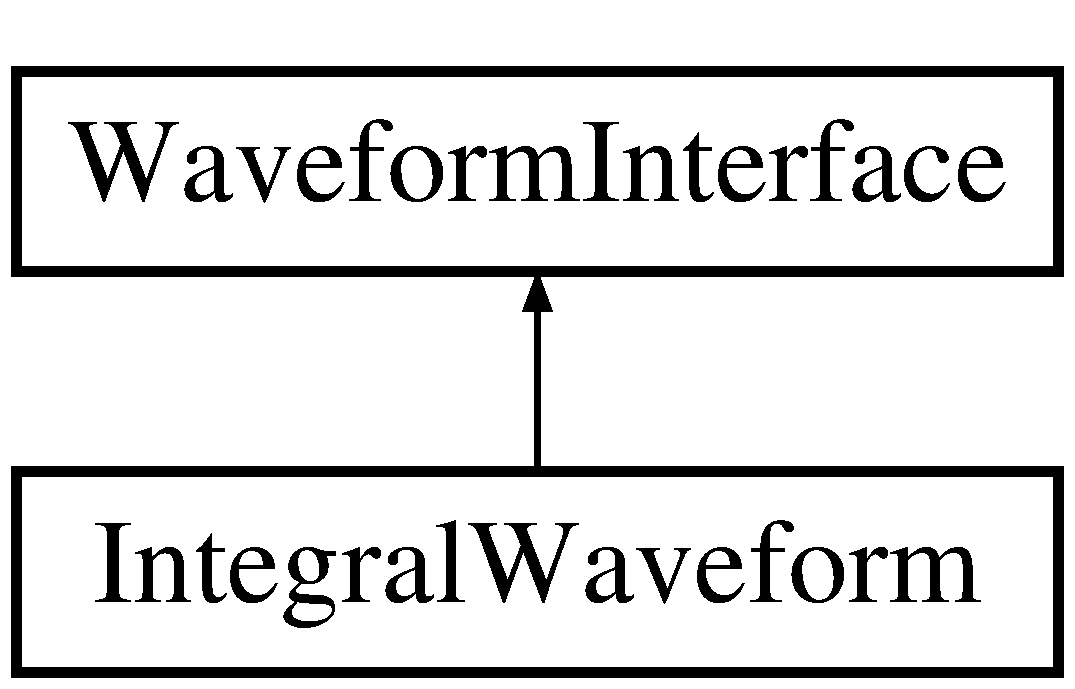
\includegraphics[height=2.000000cm]{classIntegralWaveform}
\end{center}
\end{figure}
\subsection*{Public Member Functions}
\begin{DoxyCompactItemize}
\item 
\hypertarget{classIntegralWaveform_a4586b9513a71ac52a5412402a6f39ba7}{
virtual void {\bfseries Reset} ()}
\label{classIntegralWaveform_a4586b9513a71ac52a5412402a6f39ba7}

\item 
virtual bool \hyperlink{classIntegralWaveform_a5c22fc22e29ab3589821de1bdabfe45a}{ObjectLoadSetup} (ConfigurationDataBase \&cdbData, StreamInterface $\ast$err)
\item 
virtual bool \hyperlink{classIntegralWaveform_a7b2d5fe30d954a19ac551bb9afff0124}{ProcessHttpMessage} (HttpStream \&hStream)
\item 
\hypertarget{classIntegralWaveform_a9a35249283d5fa2d0979d74315035fc9}{
virtual float {\bfseries GetValue} (int32 usecTime)}
\label{classIntegralWaveform_a9a35249283d5fa2d0979d74315035fc9}

\end{DoxyCompactItemize}


\subsection{Member Function Documentation}
\hypertarget{classIntegralWaveform_a5c22fc22e29ab3589821de1bdabfe45a}{
\index{IntegralWaveform@{IntegralWaveform}!ObjectLoadSetup@{ObjectLoadSetup}}
\index{ObjectLoadSetup@{ObjectLoadSetup}!IntegralWaveform@{IntegralWaveform}}
\subsubsection[{ObjectLoadSetup}]{\setlength{\rightskip}{0pt plus 5cm}bool IntegralWaveform::ObjectLoadSetup (
\begin{DoxyParamCaption}
\item[{ConfigurationDataBase \&}]{cdbData, }
\item[{StreamInterface $\ast$}]{err}
\end{DoxyParamCaption}
)\hspace{0.3cm}{\ttfamily  \mbox{[}virtual\mbox{]}}}}
\label{classIntegralWaveform_a5c22fc22e29ab3589821de1bdabfe45a}
Loads parameters from a CDB 
\begin{DoxyParams}{Parameters}
{\em cdbData} & the CDB \\
\hline
\end{DoxyParams}
\begin{DoxyReturn}{Returns}
True if the initialisation went ok, False otherwise 
\end{DoxyReturn}
\hypertarget{classIntegralWaveform_a7b2d5fe30d954a19ac551bb9afff0124}{
\index{IntegralWaveform@{IntegralWaveform}!ProcessHttpMessage@{ProcessHttpMessage}}
\index{ProcessHttpMessage@{ProcessHttpMessage}!IntegralWaveform@{IntegralWaveform}}
\subsubsection[{ProcessHttpMessage}]{\setlength{\rightskip}{0pt plus 5cm}bool IntegralWaveform::ProcessHttpMessage (
\begin{DoxyParamCaption}
\item[{HttpStream \&}]{hStream}
\end{DoxyParamCaption}
)\hspace{0.3cm}{\ttfamily  \mbox{[}virtual\mbox{]}}}}
\label{classIntegralWaveform_a7b2d5fe30d954a19ac551bb9afff0124}
Builds a webpage for the current object 
\begin{DoxyParams}{Parameters}
{\em hStream} & the HttpStream to write to \\
\hline
\end{DoxyParams}
\begin{DoxyReturn}{Returns}
True 
\end{DoxyReturn}


The documentation for this class was generated from the following files:\begin{DoxyCompactItemize}
\item 
IntegralWaveform.h\item 
IntegralWaveform.cpp\end{DoxyCompactItemize}

\hypertarget{classJetColormap}{
\section{JetColormap Class Reference}
\label{classJetColormap}\index{JetColormap@{JetColormap}}
}
Inheritance diagram for JetColormap:\begin{figure}[H]
\begin{center}
\leavevmode
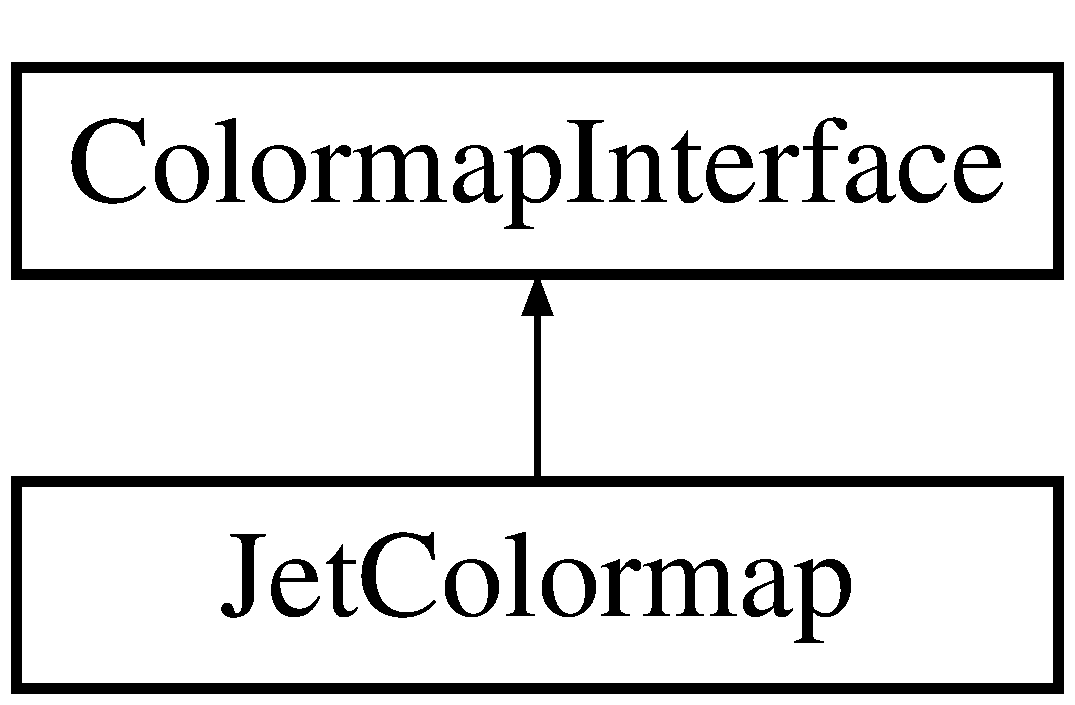
\includegraphics[height=2.000000cm]{classJetColormap}
\end{center}
\end{figure}
\subsection*{Protected Member Functions}
\begin{DoxyCompactItemize}
\item 
\hypertarget{classJetColormap_adb6098abf5cd454a5b2bd62ff8df2e6b}{
bool {\bfseries BuildJetColorMap} ()}
\label{classJetColormap_adb6098abf5cd454a5b2bd62ff8df2e6b}

\end{DoxyCompactItemize}


The documentation for this class was generated from the following files:\begin{DoxyCompactItemize}
\item 
JetColormap.h\item 
JetColormap.cpp\end{DoxyCompactItemize}

\hypertarget{classKickWaveform}{
\section{KickWaveform Class Reference}
\label{classKickWaveform}\index{KickWaveform@{KickWaveform}}
}


{\ttfamily \#include $<$KickWaveform.h$>$}

Inheritance diagram for KickWaveform:\begin{figure}[H]
\begin{center}
\leavevmode
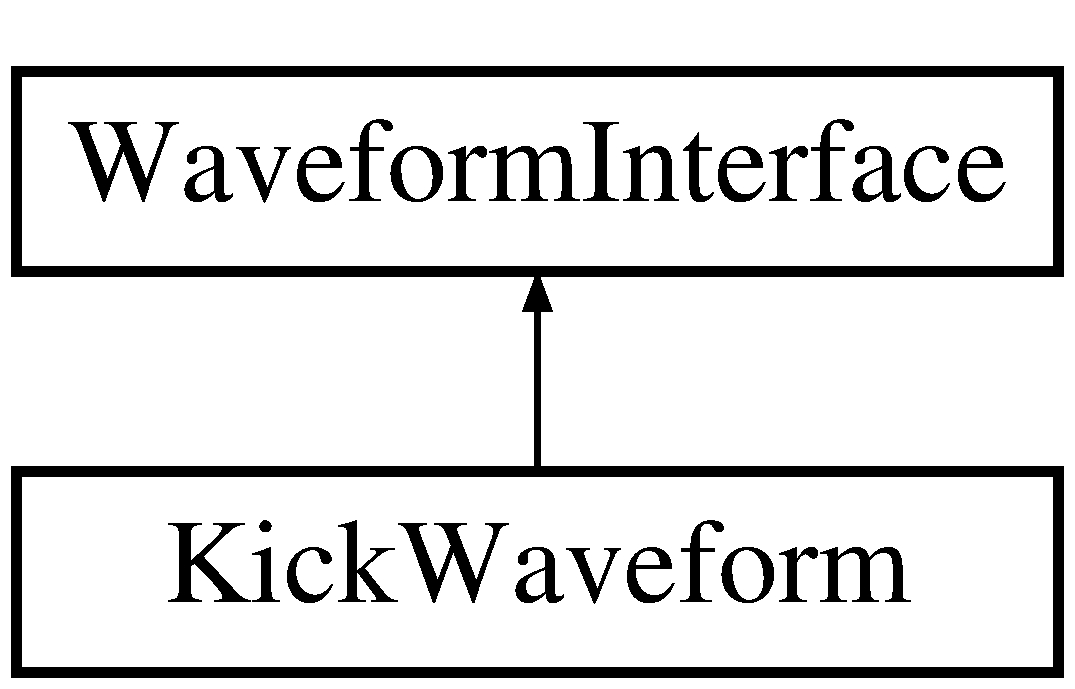
\includegraphics[height=2.000000cm]{classKickWaveform}
\end{center}
\end{figure}
\subsection*{Public Member Functions}
\begin{DoxyCompactItemize}
\item 
\hyperlink{classKickWaveform_a50fb828c1dd190b225e8e5f3631d6c36}{KickWaveform} ()
\item 
virtual \hyperlink{classKickWaveform_abe3fa01aac1a6a058630ace1744aa4f7}{$\sim$KickWaveform} ()
\item 
virtual void \hyperlink{classKickWaveform_a639370dfec04827ac91b8a38352432fa}{Reset} ()
\item 
virtual bool \hyperlink{classKickWaveform_aed9ccfd8e61b91743d2e74ac1273ffc3}{ObjectLoadSetup} (ConfigurationDataBase \&cdbData, StreamInterface $\ast$err)
\item 
virtual bool \hyperlink{classKickWaveform_a20044c2d0e8026b0957755b4128d1f92}{ProcessHttpMessage} (HttpStream \&hStream)
\item 
virtual float \hyperlink{classKickWaveform_a7a5fc20993a5a2b94481029f07a6118b}{GetValue} (int32 usecTime)
\item 
virtual int32 \hyperlink{classKickWaveform_a20cba441dd9e51c80b507a695b1b728f}{GetKickMode} ()
\item 
virtual bool \hyperlink{classKickWaveform_a65a2d2cc5a46daea138ee8212dfb9de0}{IsCompleted} (int32 relativeUsecTime)
\item 
\hypertarget{classKickWaveform_ab6d00b178ac4162f844231d85a3a8fe3}{
virtual void {\bfseries SetWindowStart} (int32 usecTime)}
\label{classKickWaveform_ab6d00b178ac4162f844231d85a3a8fe3}

\item 
\hypertarget{classKickWaveform_a88b8c9147808284eff71bd550333912b}{
void {\bfseries SetResetUsecTime} (int32 usecTime)}
\label{classKickWaveform_a88b8c9147808284eff71bd550333912b}

\end{DoxyCompactItemize}


\subsection{Detailed Description}
The Garbage Collectable and Named \hyperlink{classKickWaveform}{KickWaveform} 

\subsection{Constructor \& Destructor Documentation}
\hypertarget{classKickWaveform_a50fb828c1dd190b225e8e5f3631d6c36}{
\index{KickWaveform@{KickWaveform}!KickWaveform@{KickWaveform}}
\index{KickWaveform@{KickWaveform}!KickWaveform@{KickWaveform}}
\subsubsection[{KickWaveform}]{\setlength{\rightskip}{0pt plus 5cm}KickWaveform::KickWaveform (
\begin{DoxyParamCaption}
{}
\end{DoxyParamCaption}
)\hspace{0.3cm}{\ttfamily  \mbox{[}inline\mbox{]}}}}
\label{classKickWaveform_a50fb828c1dd190b225e8e5f3631d6c36}
Constructor \hypertarget{classKickWaveform_abe3fa01aac1a6a058630ace1744aa4f7}{
\index{KickWaveform@{KickWaveform}!$\sim$KickWaveform@{$\sim$KickWaveform}}
\index{$\sim$KickWaveform@{$\sim$KickWaveform}!KickWaveform@{KickWaveform}}
\subsubsection[{$\sim$KickWaveform}]{\setlength{\rightskip}{0pt plus 5cm}virtual KickWaveform::$\sim$KickWaveform (
\begin{DoxyParamCaption}
{}
\end{DoxyParamCaption}
)\hspace{0.3cm}{\ttfamily  \mbox{[}inline, virtual\mbox{]}}}}
\label{classKickWaveform_abe3fa01aac1a6a058630ace1744aa4f7}
Deconstructor 

\subsection{Member Function Documentation}
\hypertarget{classKickWaveform_a20cba441dd9e51c80b507a695b1b728f}{
\index{KickWaveform@{KickWaveform}!GetKickMode@{GetKickMode}}
\index{GetKickMode@{GetKickMode}!KickWaveform@{KickWaveform}}
\subsubsection[{GetKickMode}]{\setlength{\rightskip}{0pt plus 5cm}virtual int32 KickWaveform::GetKickMode (
\begin{DoxyParamCaption}
{}
\end{DoxyParamCaption}
)\hspace{0.3cm}{\ttfamily  \mbox{[}inline, virtual\mbox{]}}}}
\label{classKickWaveform_a20cba441dd9e51c80b507a695b1b728f}
Used to find out what is the KickMode of the current window \begin{DoxyReturn}{Returns}
the kick mode 
\end{DoxyReturn}
\hypertarget{classKickWaveform_a7a5fc20993a5a2b94481029f07a6118b}{
\index{KickWaveform@{KickWaveform}!GetValue@{GetValue}}
\index{GetValue@{GetValue}!KickWaveform@{KickWaveform}}
\subsubsection[{GetValue}]{\setlength{\rightskip}{0pt plus 5cm}float KickWaveform::GetValue (
\begin{DoxyParamCaption}
\item[{int32}]{usecTime}
\end{DoxyParamCaption}
)\hspace{0.3cm}{\ttfamily  \mbox{[}virtual\mbox{]}}}}
\label{classKickWaveform_a7a5fc20993a5a2b94481029f07a6118b}
Returns the value of the kickwaveform at a certain time. 
\begin{DoxyParams}{Parameters}
{\em usecTime} & current time in microseconds \\
\hline
{\em startUsecTime} & start time of the GCNKickWaveform \\
\hline
\end{DoxyParams}
\begin{DoxyReturn}{Returns}
The value of the waveform at the specified time. If usecTime is before or after the start or end time of the waveform, the first or last value is held. 
\end{DoxyReturn}


Implements \hyperlink{classWaveformInterface}{WaveformInterface}.

\hypertarget{classKickWaveform_a65a2d2cc5a46daea138ee8212dfb9de0}{
\index{KickWaveform@{KickWaveform}!IsCompleted@{IsCompleted}}
\index{IsCompleted@{IsCompleted}!KickWaveform@{KickWaveform}}
\subsubsection[{IsCompleted}]{\setlength{\rightskip}{0pt plus 5cm}virtual bool KickWaveform::IsCompleted (
\begin{DoxyParamCaption}
\item[{int32}]{relativeUsecTime}
\end{DoxyParamCaption}
)\hspace{0.3cm}{\ttfamily  \mbox{[}inline, virtual\mbox{]}}}}
\label{classKickWaveform_a65a2d2cc5a46daea138ee8212dfb9de0}
Used to find out if the \hyperlink{classKickWaveform}{KickWaveform} is completed 
\begin{DoxyParams}{Parameters}
{\em usecTime} & current time in microseconds \\
\hline
{\em startUsecTime} & start time of the GCNKickWaveform \\
\hline
\end{DoxyParams}
\begin{DoxyReturn}{Returns}
True if the \hyperlink{classKickWaveform}{KickWaveform} (for the given startUsecTime and usecTime is completed, False otherwise 
\end{DoxyReturn}
\hypertarget{classKickWaveform_aed9ccfd8e61b91743d2e74ac1273ffc3}{
\index{KickWaveform@{KickWaveform}!ObjectLoadSetup@{ObjectLoadSetup}}
\index{ObjectLoadSetup@{ObjectLoadSetup}!KickWaveform@{KickWaveform}}
\subsubsection[{ObjectLoadSetup}]{\setlength{\rightskip}{0pt plus 5cm}bool KickWaveform::ObjectLoadSetup (
\begin{DoxyParamCaption}
\item[{ConfigurationDataBase \&}]{cdbData, }
\item[{StreamInterface $\ast$}]{err}
\end{DoxyParamCaption}
)\hspace{0.3cm}{\ttfamily  \mbox{[}virtual\mbox{]}}}}
\label{classKickWaveform_aed9ccfd8e61b91743d2e74ac1273ffc3}
Loads parameters from a CDB 
\begin{DoxyParams}{Parameters}
{\em cdbData} & the CDB \\
\hline
\end{DoxyParams}
\begin{DoxyReturn}{Returns}
True if the initialisation went ok, False otherwise 
\end{DoxyReturn}
\hypertarget{classKickWaveform_a20044c2d0e8026b0957755b4128d1f92}{
\index{KickWaveform@{KickWaveform}!ProcessHttpMessage@{ProcessHttpMessage}}
\index{ProcessHttpMessage@{ProcessHttpMessage}!KickWaveform@{KickWaveform}}
\subsubsection[{ProcessHttpMessage}]{\setlength{\rightskip}{0pt plus 5cm}bool KickWaveform::ProcessHttpMessage (
\begin{DoxyParamCaption}
\item[{HttpStream \&}]{hStream}
\end{DoxyParamCaption}
)\hspace{0.3cm}{\ttfamily  \mbox{[}virtual\mbox{]}}}}
\label{classKickWaveform_a20044c2d0e8026b0957755b4128d1f92}
Builds a webpage for the current object 
\begin{DoxyParams}{Parameters}
{\em hStream} & the HttpStream to write to \\
\hline
\end{DoxyParams}
\begin{DoxyReturn}{Returns}
True 
\end{DoxyReturn}
\hypertarget{classKickWaveform_a639370dfec04827ac91b8a38352432fa}{
\index{KickWaveform@{KickWaveform}!Reset@{Reset}}
\index{Reset@{Reset}!KickWaveform@{KickWaveform}}
\subsubsection[{Reset}]{\setlength{\rightskip}{0pt plus 5cm}virtual void KickWaveform::Reset (
\begin{DoxyParamCaption}
{}
\end{DoxyParamCaption}
)\hspace{0.3cm}{\ttfamily  \mbox{[}inline, virtual\mbox{]}}}}
\label{classKickWaveform_a639370dfec04827ac91b8a38352432fa}
Reset function. Resets the internal states and waveforms. To be called in the PREPULSE phase. 

Implements \hyperlink{classWaveformInterface}{WaveformInterface}.



The documentation for this class was generated from the following files:\begin{DoxyCompactItemize}
\item 
\hyperlink{KickWaveform_8h}{KickWaveform.h}\item 
KickWaveform.cpp\end{DoxyCompactItemize}

\hypertarget{structKickWindow}{
\section{KickWindow Struct Reference}
\label{structKickWindow}\index{KickWindow@{KickWindow}}
}


{\ttfamily \#include $<$KickWaveform.h$>$}

\subsection*{Public Attributes}
\begin{DoxyCompactItemize}
\item 
int32 \hyperlink{structKickWindow_ab7d5f6704ca1b06adcce2fbbd28fd0bd}{usecLength}
\item 
float \hyperlink{structKickWindow_a19abd0bca8e2503f7d6e2eac912071b6}{amplitude}
\item 
\hyperlink{structKWStatusBitfield}{KWStatusBitfield} \hyperlink{structKickWindow_ad9a832cfa230098138426e8cd7ac18b6}{status}
\item 
GCRTemplate$<$ \hyperlink{classWaveformInterface}{WaveformInterface} $>$ \hyperlink{structKickWindow_ac35a8cd53ad6c399fa7abfea65d5a0eb}{deltaTwaveform}
\end{DoxyCompactItemize}


\subsection{Detailed Description}
Structure representing a single element in a GCNKickWaveform 

\subsection{Member Data Documentation}
\hypertarget{structKickWindow_a19abd0bca8e2503f7d6e2eac912071b6}{
\index{KickWindow@{KickWindow}!amplitude@{amplitude}}
\index{amplitude@{amplitude}!KickWindow@{KickWindow}}
\subsubsection[{amplitude}]{\setlength{\rightskip}{0pt plus 5cm}float {\bf KickWindow::amplitude}}}
\label{structKickWindow_a19abd0bca8e2503f7d6e2eac912071b6}
Amplitude \hypertarget{structKickWindow_ac35a8cd53ad6c399fa7abfea65d5a0eb}{
\index{KickWindow@{KickWindow}!deltaTwaveform@{deltaTwaveform}}
\index{deltaTwaveform@{deltaTwaveform}!KickWindow@{KickWindow}}
\subsubsection[{deltaTwaveform}]{\setlength{\rightskip}{0pt plus 5cm}GCRTemplate$<${\bf WaveformInterface}$>$ {\bf KickWindow::deltaTwaveform}}}
\label{structKickWindow_ac35a8cd53ad6c399fa7abfea65d5a0eb}
The window associated waveform \hypertarget{structKickWindow_ad9a832cfa230098138426e8cd7ac18b6}{
\index{KickWindow@{KickWindow}!status@{status}}
\index{status@{status}!KickWindow@{KickWindow}}
\subsubsection[{status}]{\setlength{\rightskip}{0pt plus 5cm}{\bf KWStatusBitfield} {\bf KickWindow::status}}}
\label{structKickWindow_ad9a832cfa230098138426e8cd7ac18b6}
Status bitfield \hypertarget{structKickWindow_ab7d5f6704ca1b06adcce2fbbd28fd0bd}{
\index{KickWindow@{KickWindow}!usecLength@{usecLength}}
\index{usecLength@{usecLength}!KickWindow@{KickWindow}}
\subsubsection[{usecLength}]{\setlength{\rightskip}{0pt plus 5cm}int32 {\bf KickWindow::usecLength}}}
\label{structKickWindow_ab7d5f6704ca1b06adcce2fbbd28fd0bd}
Length of the kick window 

The documentation for this struct was generated from the following file:\begin{DoxyCompactItemize}
\item 
\hyperlink{KickWaveform_8h}{KickWaveform.h}\end{DoxyCompactItemize}

\hypertarget{structKWStatusBitfield}{
\section{KWStatusBitfield Struct Reference}
\label{structKWStatusBitfield}\index{KWStatusBitfield@{KWStatusBitfield}}
}


{\ttfamily \#include $<$KickWaveform.h$>$}

\subsection*{Public Attributes}
\begin{DoxyCompactItemize}
\item 
unsigned int \hyperlink{structKWStatusBitfield_a75cbbaa8beb9ceed559a03c13c04803b}{kickMode}:2
\end{DoxyCompactItemize}


\subsection{Detailed Description}
The GCNKickWindow's bitfield 

\subsection{Member Data Documentation}
\hypertarget{structKWStatusBitfield_a75cbbaa8beb9ceed559a03c13c04803b}{
\index{KWStatusBitfield@{KWStatusBitfield}!kickMode@{kickMode}}
\index{kickMode@{kickMode}!KWStatusBitfield@{KWStatusBitfield}}
\subsubsection[{kickMode}]{\setlength{\rightskip}{0pt plus 5cm}unsigned int {\bf KWStatusBitfield::kickMode}}}
\label{structKWStatusBitfield_a75cbbaa8beb9ceed559a03c13c04803b}
Specify if a GCNKickWindow is off, additive or substitutive 

The documentation for this struct was generated from the following file:\begin{DoxyCompactItemize}
\item 
\hyperlink{KickWaveform_8h}{KickWaveform.h}\end{DoxyCompactItemize}

\hypertarget{classMatlabConverter}{
\section{MatlabConverter Class Reference}
\label{classMatlabConverter}\index{MatlabConverter@{MatlabConverter}}
}
\subsection*{Public Member Functions}
\begin{DoxyCompactItemize}
\item 
\hyperlink{classMatlabConverter_ae231df5f9ce670b05ad9025084e7ee48}{MatlabConverter} (Streamable $\ast$out)
\item 
int \hyperlink{classMatlabConverter_a41c2cbd92d7f8c9ad4f5f2cff09ba3c6}{CalculateDimension} (MatrixF \&mat, const char $\ast$variableName)
\item 
int \hyperlink{classMatlabConverter_aaf250197b07b0ea5c03b5227736947ee}{CalculateDimension} (MatrixD \&mat, const char $\ast$variableName)
\item 
int \hyperlink{classMatlabConverter_ae19203f53f8ec927af2c949f2f59b194}{CalculateDimension} (MatrixI \&mat, const char $\ast$variableName)
\item 
int \hyperlink{classMatlabConverter_a4abba9a7dd19d6b3c66934c2448c3825}{CalculateDimension} (const char $\ast$$\ast$listOfStrings, int nStrings, const char $\ast$variableName)
\item 
int \hyperlink{classMatlabConverter_a0eec9381ea2acc2fc13bd1c8fdac680c}{CalculateDimensionFloat} (const char $\ast$variableName)
\item 
int \hyperlink{classMatlabConverter_ade1e325d7a5ecc800959631d424431d2}{CalculateDimensionDouble} (const char $\ast$variableName)
\item 
bool \hyperlink{classMatlabConverter_a5d72106d3b7ae4cfa2c4109b18b8bd17}{Save} (float value, const char $\ast$variableName)
\item 
bool \hyperlink{classMatlabConverter_afa0e6c9e09a491717d5229e4b08d15b0}{Save} (double value, const char $\ast$variableName)
\item 
bool \hyperlink{classMatlabConverter_aa02883e0f36920d6e5baa1acafe48b2f}{Save} (MatrixF \&mat, const char $\ast$variableName)
\item 
bool \hyperlink{classMatlabConverter_a98c7d90bf3257d2ab9737b8823570b0f}{Save} (MatrixD \&mat, const char $\ast$variableName)
\item 
bool \hyperlink{classMatlabConverter_a1b7aaf580f2edfea7d41ac1d8ffd8d39}{Save} (MatrixI \&mat, const char $\ast$variableName)
\item 
bool \hyperlink{classMatlabConverter_aeab22d25ec1b0550cfd7de1b401f32a6}{Save} (const char $\ast$$\ast$listOfStrings, int nStrings, const char $\ast$variableName)
\item 
bool \hyperlink{classMatlabConverter_aeef921aa4ec5d6e6a5d02fda1a84422f}{InitStructure} (const char $\ast$nameStruct, const char $\ast$$\ast$listField, int nFields, int totalDimension)
\item 
bool \hyperlink{classMatlabConverter_aa4122955ba117021dc9d08d148ed31ed}{InitCell} (const char $\ast$nameCell, int nFields, int totalDimension)
\end{DoxyCompactItemize}
\subsection*{Friends}
\begin{DoxyCompactItemize}
\item 
\hypertarget{classMatlabConverter_a0bbc5f54e71e79c28941ea3bf59472ff}{
bool {\bfseries MCSaveF} (\hyperlink{classMatlabConverter}{MatlabConverter} \&mc, float value, const char $\ast$variableName)}
\label{classMatlabConverter_a0bbc5f54e71e79c28941ea3bf59472ff}

\item 
\hypertarget{classMatlabConverter_a47bf295200d42fd7f28923fd6e1acaa3}{
bool {\bfseries MCSaveD} (\hyperlink{classMatlabConverter}{MatlabConverter} \&mc, double value, const char $\ast$variableName)}
\label{classMatlabConverter_a47bf295200d42fd7f28923fd6e1acaa3}

\item 
\hypertarget{classMatlabConverter_aa8c8d361346d6aa95488c2582d3a9c20}{
bool {\bfseries MCSaveMF} (\hyperlink{classMatlabConverter}{MatlabConverter} \&mc, MatrixF \&mat, const char $\ast$variableName)}
\label{classMatlabConverter_aa8c8d361346d6aa95488c2582d3a9c20}

\item 
bool \hyperlink{classMatlabConverter_a10f6a83594f4db66392e6f5f3661e570}{MCSaveMD} (\hyperlink{classMatlabConverter}{MatlabConverter} \&mc, MatrixD \&mat, const char $\ast$variableName)
\item 
\hypertarget{classMatlabConverter_a7aaec595471ddd504f18d7fbc57d1d99}{
bool {\bfseries MCSaveMI} (\hyperlink{classMatlabConverter}{MatlabConverter} \&mc, MatrixI \&mat, const char $\ast$variableName)}
\label{classMatlabConverter_a7aaec595471ddd504f18d7fbc57d1d99}

\item 
bool \hyperlink{classMatlabConverter_a885c79a3a662eef92348655319e90e47}{MCSaveS} (\hyperlink{classMatlabConverter}{MatlabConverter} \&mc, const char $\ast$$\ast$listOfStrings, int nStrings, const char $\ast$variableName)
\end{DoxyCompactItemize}


\subsection{Constructor \& Destructor Documentation}
\hypertarget{classMatlabConverter_ae231df5f9ce670b05ad9025084e7ee48}{
\index{MatlabConverter@{MatlabConverter}!MatlabConverter@{MatlabConverter}}
\index{MatlabConverter@{MatlabConverter}!MatlabConverter@{MatlabConverter}}
\subsubsection[{MatlabConverter}]{\setlength{\rightskip}{0pt plus 5cm}MatlabConverter::MatlabConverter (
\begin{DoxyParamCaption}
\item[{Streamable $\ast$}]{out}
\end{DoxyParamCaption}
)\hspace{0.3cm}{\ttfamily  \mbox{[}inline\mbox{]}}}}
\label{classMatlabConverter_ae231df5f9ce670b05ad9025084e7ee48}


\subsection{Member Function Documentation}
\hypertarget{classMatlabConverter_a41c2cbd92d7f8c9ad4f5f2cff09ba3c6}{
\index{MatlabConverter@{MatlabConverter}!CalculateDimension@{CalculateDimension}}
\index{CalculateDimension@{CalculateDimension}!MatlabConverter@{MatlabConverter}}
\subsubsection[{CalculateDimension}]{\setlength{\rightskip}{0pt plus 5cm}int MatlabConverter::CalculateDimension (
\begin{DoxyParamCaption}
\item[{MatrixF \&}]{mat, }
\item[{const char $\ast$}]{variableName}
\end{DoxyParamCaption}
)}}
\label{classMatlabConverter_a41c2cbd92d7f8c9ad4f5f2cff09ba3c6}
\hypertarget{classMatlabConverter_aaf250197b07b0ea5c03b5227736947ee}{
\index{MatlabConverter@{MatlabConverter}!CalculateDimension@{CalculateDimension}}
\index{CalculateDimension@{CalculateDimension}!MatlabConverter@{MatlabConverter}}
\subsubsection[{CalculateDimension}]{\setlength{\rightskip}{0pt plus 5cm}int MatlabConverter::CalculateDimension (
\begin{DoxyParamCaption}
\item[{MatrixD \&}]{mat, }
\item[{const char $\ast$}]{variableName}
\end{DoxyParamCaption}
)}}
\label{classMatlabConverter_aaf250197b07b0ea5c03b5227736947ee}
\hypertarget{classMatlabConverter_a4abba9a7dd19d6b3c66934c2448c3825}{
\index{MatlabConverter@{MatlabConverter}!CalculateDimension@{CalculateDimension}}
\index{CalculateDimension@{CalculateDimension}!MatlabConverter@{MatlabConverter}}
\subsubsection[{CalculateDimension}]{\setlength{\rightskip}{0pt plus 5cm}int MatlabConverter::CalculateDimension (
\begin{DoxyParamCaption}
\item[{const char $\ast$$\ast$}]{listOfStrings, }
\item[{int}]{nStrings, }
\item[{const char $\ast$}]{variableName}
\end{DoxyParamCaption}
)}}
\label{classMatlabConverter_a4abba9a7dd19d6b3c66934c2448c3825}
\hypertarget{classMatlabConverter_ae19203f53f8ec927af2c949f2f59b194}{
\index{MatlabConverter@{MatlabConverter}!CalculateDimension@{CalculateDimension}}
\index{CalculateDimension@{CalculateDimension}!MatlabConverter@{MatlabConverter}}
\subsubsection[{CalculateDimension}]{\setlength{\rightskip}{0pt plus 5cm}int MatlabConverter::CalculateDimension (
\begin{DoxyParamCaption}
\item[{MatrixI \&}]{mat, }
\item[{const char $\ast$}]{variableName}
\end{DoxyParamCaption}
)}}
\label{classMatlabConverter_ae19203f53f8ec927af2c949f2f59b194}
\hypertarget{classMatlabConverter_ade1e325d7a5ecc800959631d424431d2}{
\index{MatlabConverter@{MatlabConverter}!CalculateDimensionDouble@{CalculateDimensionDouble}}
\index{CalculateDimensionDouble@{CalculateDimensionDouble}!MatlabConverter@{MatlabConverter}}
\subsubsection[{CalculateDimensionDouble}]{\setlength{\rightskip}{0pt plus 5cm}int MatlabConverter::CalculateDimensionDouble (
\begin{DoxyParamCaption}
\item[{const char $\ast$}]{variableName}
\end{DoxyParamCaption}
)}}
\label{classMatlabConverter_ade1e325d7a5ecc800959631d424431d2}
\hypertarget{classMatlabConverter_a0eec9381ea2acc2fc13bd1c8fdac680c}{
\index{MatlabConverter@{MatlabConverter}!CalculateDimensionFloat@{CalculateDimensionFloat}}
\index{CalculateDimensionFloat@{CalculateDimensionFloat}!MatlabConverter@{MatlabConverter}}
\subsubsection[{CalculateDimensionFloat}]{\setlength{\rightskip}{0pt plus 5cm}int MatlabConverter::CalculateDimensionFloat (
\begin{DoxyParamCaption}
\item[{const char $\ast$}]{variableName}
\end{DoxyParamCaption}
)}}
\label{classMatlabConverter_a0eec9381ea2acc2fc13bd1c8fdac680c}
\hypertarget{classMatlabConverter_aa4122955ba117021dc9d08d148ed31ed}{
\index{MatlabConverter@{MatlabConverter}!InitCell@{InitCell}}
\index{InitCell@{InitCell}!MatlabConverter@{MatlabConverter}}
\subsubsection[{InitCell}]{\setlength{\rightskip}{0pt plus 5cm}bool MatlabConverter::InitCell (
\begin{DoxyParamCaption}
\item[{const char $\ast$}]{nameCell, }
\item[{int}]{nFields, }
\item[{int}]{totalDimension}
\end{DoxyParamCaption}
)}}
\label{classMatlabConverter_aa4122955ba117021dc9d08d148ed31ed}
\hypertarget{classMatlabConverter_aeef921aa4ec5d6e6a5d02fda1a84422f}{
\index{MatlabConverter@{MatlabConverter}!InitStructure@{InitStructure}}
\index{InitStructure@{InitStructure}!MatlabConverter@{MatlabConverter}}
\subsubsection[{InitStructure}]{\setlength{\rightskip}{0pt plus 5cm}bool MatlabConverter::InitStructure (
\begin{DoxyParamCaption}
\item[{const char $\ast$}]{nameStruct, }
\item[{const char $\ast$$\ast$}]{listField, }
\item[{int}]{nFields, }
\item[{int}]{totalDimension}
\end{DoxyParamCaption}
)}}
\label{classMatlabConverter_aeef921aa4ec5d6e6a5d02fda1a84422f}
\hypertarget{classMatlabConverter_a1b7aaf580f2edfea7d41ac1d8ffd8d39}{
\index{MatlabConverter@{MatlabConverter}!Save@{Save}}
\index{Save@{Save}!MatlabConverter@{MatlabConverter}}
\subsubsection[{Save}]{\setlength{\rightskip}{0pt plus 5cm}bool MatlabConverter::Save (
\begin{DoxyParamCaption}
\item[{MatrixI \&}]{mat, }
\item[{const char $\ast$}]{variableName}
\end{DoxyParamCaption}
)\hspace{0.3cm}{\ttfamily  \mbox{[}inline\mbox{]}}}}
\label{classMatlabConverter_a1b7aaf580f2edfea7d41ac1d8ffd8d39}
\hypertarget{classMatlabConverter_aeab22d25ec1b0550cfd7de1b401f32a6}{
\index{MatlabConverter@{MatlabConverter}!Save@{Save}}
\index{Save@{Save}!MatlabConverter@{MatlabConverter}}
\subsubsection[{Save}]{\setlength{\rightskip}{0pt plus 5cm}bool MatlabConverter::Save (
\begin{DoxyParamCaption}
\item[{const char $\ast$$\ast$}]{listOfStrings, }
\item[{int}]{nStrings, }
\item[{const char $\ast$}]{variableName}
\end{DoxyParamCaption}
)\hspace{0.3cm}{\ttfamily  \mbox{[}inline\mbox{]}}}}
\label{classMatlabConverter_aeab22d25ec1b0550cfd7de1b401f32a6}
\hypertarget{classMatlabConverter_a98c7d90bf3257d2ab9737b8823570b0f}{
\index{MatlabConverter@{MatlabConverter}!Save@{Save}}
\index{Save@{Save}!MatlabConverter@{MatlabConverter}}
\subsubsection[{Save}]{\setlength{\rightskip}{0pt plus 5cm}bool MatlabConverter::Save (
\begin{DoxyParamCaption}
\item[{MatrixD \&}]{mat, }
\item[{const char $\ast$}]{variableName}
\end{DoxyParamCaption}
)\hspace{0.3cm}{\ttfamily  \mbox{[}inline\mbox{]}}}}
\label{classMatlabConverter_a98c7d90bf3257d2ab9737b8823570b0f}
\hypertarget{classMatlabConverter_a5d72106d3b7ae4cfa2c4109b18b8bd17}{
\index{MatlabConverter@{MatlabConverter}!Save@{Save}}
\index{Save@{Save}!MatlabConverter@{MatlabConverter}}
\subsubsection[{Save}]{\setlength{\rightskip}{0pt plus 5cm}bool MatlabConverter::Save (
\begin{DoxyParamCaption}
\item[{float}]{value, }
\item[{const char $\ast$}]{variableName}
\end{DoxyParamCaption}
)\hspace{0.3cm}{\ttfamily  \mbox{[}inline\mbox{]}}}}
\label{classMatlabConverter_a5d72106d3b7ae4cfa2c4109b18b8bd17}
\hypertarget{classMatlabConverter_aa02883e0f36920d6e5baa1acafe48b2f}{
\index{MatlabConverter@{MatlabConverter}!Save@{Save}}
\index{Save@{Save}!MatlabConverter@{MatlabConverter}}
\subsubsection[{Save}]{\setlength{\rightskip}{0pt plus 5cm}bool MatlabConverter::Save (
\begin{DoxyParamCaption}
\item[{MatrixF \&}]{mat, }
\item[{const char $\ast$}]{variableName}
\end{DoxyParamCaption}
)\hspace{0.3cm}{\ttfamily  \mbox{[}inline\mbox{]}}}}
\label{classMatlabConverter_aa02883e0f36920d6e5baa1acafe48b2f}
\hypertarget{classMatlabConverter_afa0e6c9e09a491717d5229e4b08d15b0}{
\index{MatlabConverter@{MatlabConverter}!Save@{Save}}
\index{Save@{Save}!MatlabConverter@{MatlabConverter}}
\subsubsection[{Save}]{\setlength{\rightskip}{0pt plus 5cm}bool MatlabConverter::Save (
\begin{DoxyParamCaption}
\item[{double}]{value, }
\item[{const char $\ast$}]{variableName}
\end{DoxyParamCaption}
)\hspace{0.3cm}{\ttfamily  \mbox{[}inline\mbox{]}}}}
\label{classMatlabConverter_afa0e6c9e09a491717d5229e4b08d15b0}


\subsection{Friends And Related Function Documentation}
\hypertarget{classMatlabConverter_a10f6a83594f4db66392e6f5f3661e570}{
\index{MatlabConverter@{MatlabConverter}!MCSaveMD@{MCSaveMD}}
\index{MCSaveMD@{MCSaveMD}!MatlabConverter@{MatlabConverter}}
\subsubsection[{MCSaveMD}]{\setlength{\rightskip}{0pt plus 5cm}bool MCSaveMD (
\begin{DoxyParamCaption}
\item[{{\bf MatlabConverter} \&}]{mc, }
\item[{MatrixD \&}]{mat, }
\item[{const char $\ast$}]{variableName}
\end{DoxyParamCaption}
)\hspace{0.3cm}{\ttfamily  \mbox{[}friend\mbox{]}}}}
\label{classMatlabConverter_a10f6a83594f4db66392e6f5f3661e570}
\hypertarget{classMatlabConverter_a885c79a3a662eef92348655319e90e47}{
\index{MatlabConverter@{MatlabConverter}!MCSaveS@{MCSaveS}}
\index{MCSaveS@{MCSaveS}!MatlabConverter@{MatlabConverter}}
\subsubsection[{MCSaveS}]{\setlength{\rightskip}{0pt plus 5cm}bool MCSaveS (
\begin{DoxyParamCaption}
\item[{{\bf MatlabConverter} \&}]{mc, }
\item[{const char $\ast$$\ast$}]{listOfStrings, }
\item[{int}]{nStrings, }
\item[{const char $\ast$}]{variableName}
\end{DoxyParamCaption}
)\hspace{0.3cm}{\ttfamily  \mbox{[}friend\mbox{]}}}}
\label{classMatlabConverter_a885c79a3a662eef92348655319e90e47}


The documentation for this class was generated from the following files:\begin{DoxyCompactItemize}
\item 
MatlabConverter.h\item 
MatlabConverter.cpp\end{DoxyCompactItemize}

\hypertarget{classMatrixRow}{
\section{MatrixRow$<$ T $>$ Class Template Reference}
\label{classMatrixRow}\index{MatrixRow@{MatrixRow}}
}


{\ttfamily \#include $<$Matrix.h$>$}

\subsection*{Public Member Functions}
\begin{DoxyCompactItemize}
\item 
\hyperlink{classMatrixRow_a0baa60140156c97c8a011dfe2f1c88f5}{MatrixRow} (T $\ast$row, int m)
\item 
T \& \hyperlink{classMatrixRow_a83e92de3600d6f5393403075c1b1d89f}{operator\mbox{[}$\,$\mbox{]}} (int col) const 
\end{DoxyCompactItemize}


\subsection{Detailed Description}
\subsubsection*{template$<$class T$>$class MatrixRow$<$ T $>$}

a row of th ematrix 

\subsection{Constructor \& Destructor Documentation}
\hypertarget{classMatrixRow_a0baa60140156c97c8a011dfe2f1c88f5}{
\index{MatrixRow@{MatrixRow}!MatrixRow@{MatrixRow}}
\index{MatrixRow@{MatrixRow}!MatrixRow@{MatrixRow}}
\subsubsection[{MatrixRow}]{\setlength{\rightskip}{0pt plus 5cm}template$<$class T$>$ {\bf MatrixRow}$<$ T $>$::{\bf MatrixRow} (
\begin{DoxyParamCaption}
\item[{T $\ast$}]{row, }
\item[{int}]{m}
\end{DoxyParamCaption}
)\hspace{0.3cm}{\ttfamily  \mbox{[}inline\mbox{]}}}}
\label{classMatrixRow_a0baa60140156c97c8a011dfe2f1c88f5}


\subsection{Member Function Documentation}
\hypertarget{classMatrixRow_a83e92de3600d6f5393403075c1b1d89f}{
\index{MatrixRow@{MatrixRow}!operator\mbox{[}\mbox{]}@{operator[]}}
\index{operator\mbox{[}\mbox{]}@{operator[]}!MatrixRow@{MatrixRow}}
\subsubsection[{operator[]}]{\setlength{\rightskip}{0pt plus 5cm}template$<$class T$>$ T\& {\bf MatrixRow}$<$ T $>$::operator\mbox{[}$\,$\mbox{]} (
\begin{DoxyParamCaption}
\item[{int}]{col}
\end{DoxyParamCaption}
) const\hspace{0.3cm}{\ttfamily  \mbox{[}inline\mbox{]}}}}
\label{classMatrixRow_a83e92de3600d6f5393403075c1b1d89f}


The documentation for this class was generated from the following file:\begin{DoxyCompactItemize}
\item 
\hyperlink{Matrix_8h}{Matrix.h}\end{DoxyCompactItemize}

\hypertarget{classMatrixT}{
\section{MatrixT$<$ T $>$ Class Template Reference}
\label{classMatrixT}\index{MatrixT@{MatrixT}}
}


{\ttfamily \#include $<$Matrix.h$>$}

Inheritance diagram for MatrixT$<$ T $>$:\begin{figure}[H]
\begin{center}
\leavevmode
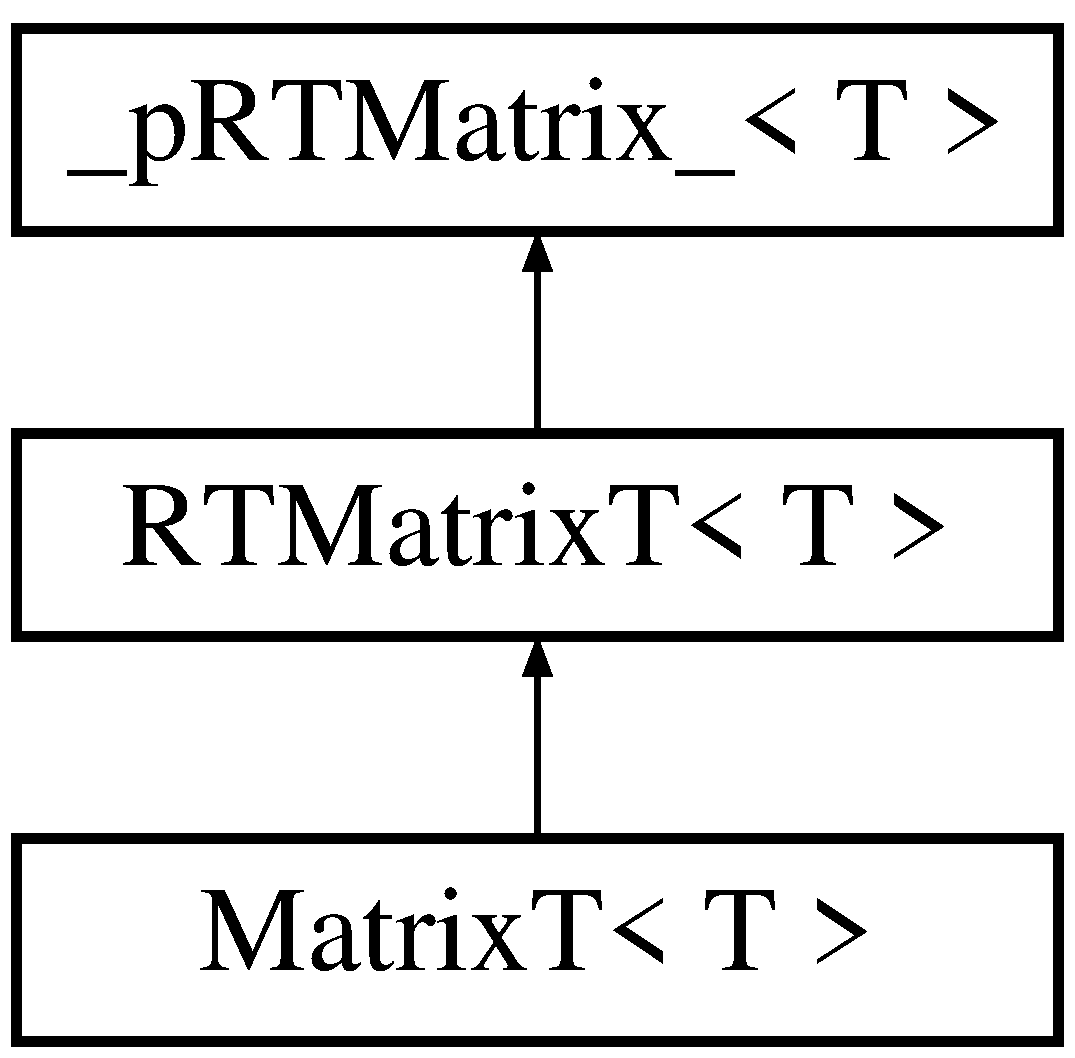
\includegraphics[height=3.000000cm]{classMatrixT}
\end{center}
\end{figure}
\subsection*{Public Member Functions}
\begin{DoxyCompactItemize}
\item 
void \hyperlink{classMatrixT_a714fbd6bfdec6d76066eae21e86f693c}{ReSize} (uint32 nRows, uint32 nColumns)
\item 
\hyperlink{classMatrixT_ab9d90c99b98b11471a01695b145c6415}{MatrixT} ()
\item 
\hyperlink{classMatrixT_a1273ec656bc69793f67e7feccdfd37f6}{MatrixT} (uint32 nRows, uint32 nColumns)
\item 
\hyperlink{classMatrixT_a0619cdab01425d05a7f2bb2d253091f5}{MatrixT} (uint32 nRows, uint32 nColumns, const T $\ast$source)
\item 
\hyperlink{classMatrixT_abbdff52c78a71a6d1a743f07f08c525e}{MatrixT} (const \hyperlink{classRTMatrixT}{RTMatrixT}$<$ T $>$ \&A)
\item 
\hyperlink{classMatrixT_aceea7e277d78309b8934a0b93e13c904}{MatrixT} (const \hyperlink{classMatrixT}{MatrixT} \&A)
\item 
\hyperlink{classMatrixT_a8292b69becb7cf206d75e699767e68b3}{$\sim$MatrixT} ()
\item 
\hyperlink{classMatrixT}{MatrixT} \& \hyperlink{classMatrixT_a157b5b4b281c2ab15a5e0797150e6a5d}{operator=} (const \hyperlink{classRTMatrixT}{RTMatrixT}$<$ T $>$ \&A)
\item 
\hyperlink{classMatrixT}{MatrixT} \& \hyperlink{classMatrixT_afe5a46a81564d716c0a70cb14aff80c9}{operator=} (const \hyperlink{classMatrixT}{MatrixT}$<$ T $>$ \&A)
\item 
const \hyperlink{classMatrixRow}{MatrixRow}$<$ T $>$ \hyperlink{classMatrixT_a8c84047f97f2d07290a7882884e50397}{operator\mbox{[}$\,$\mbox{]}} (int rowNo)
\item 
bool \hyperlink{classMatrixT_a34f8d56e92dad7d8eafd64afcd3c81f4}{operator$\ast$=} (const \hyperlink{classRTMatrixT}{RTMatrixT}$<$ T $>$ \&A)
\item 
void \hyperlink{classMatrixT_adc5f8700b8cdab6c65b3659b90eb550c}{operator$\ast$=} (T x)
\item 
bool const \hyperlink{classMatrixT_a3383eabbe87a7ebe255b3d409f005f9d}{operator+=} (const \hyperlink{classRTMatrixT}{RTMatrixT}$<$ T $>$ \&A)
\item 
bool \hyperlink{classMatrixT_a87aae833ab29686ae8bbaab0cb9c379f}{operator-\/=} (const \hyperlink{classRTMatrixT}{RTMatrixT}$<$ T $>$ \&A)
\end{DoxyCompactItemize}


\subsection{Detailed Description}
\subsubsection*{template$<$class T$>$class MatrixT$<$ T $>$}

this is an extension of RTMatrix with algebraic capabilities 

\subsection{Constructor \& Destructor Documentation}
\hypertarget{classMatrixT_ab9d90c99b98b11471a01695b145c6415}{
\index{MatrixT@{MatrixT}!MatrixT@{MatrixT}}
\index{MatrixT@{MatrixT}!MatrixT@{MatrixT}}
\subsubsection[{MatrixT}]{\setlength{\rightskip}{0pt plus 5cm}template$<$class T$>$ {\bf MatrixT}$<$ T $>$::{\bf MatrixT} (
\begin{DoxyParamCaption}
{}
\end{DoxyParamCaption}
)\hspace{0.3cm}{\ttfamily  \mbox{[}inline\mbox{]}}}}
\label{classMatrixT_ab9d90c99b98b11471a01695b145c6415}
\hypertarget{classMatrixT_a1273ec656bc69793f67e7feccdfd37f6}{
\index{MatrixT@{MatrixT}!MatrixT@{MatrixT}}
\index{MatrixT@{MatrixT}!MatrixT@{MatrixT}}
\subsubsection[{MatrixT}]{\setlength{\rightskip}{0pt plus 5cm}template$<$class T$>$ {\bf MatrixT}$<$ T $>$::{\bf MatrixT} (
\begin{DoxyParamCaption}
\item[{uint32}]{nRows, }
\item[{uint32}]{nColumns}
\end{DoxyParamCaption}
)\hspace{0.3cm}{\ttfamily  \mbox{[}inline\mbox{]}}}}
\label{classMatrixT_a1273ec656bc69793f67e7feccdfd37f6}
\hypertarget{classMatrixT_a0619cdab01425d05a7f2bb2d253091f5}{
\index{MatrixT@{MatrixT}!MatrixT@{MatrixT}}
\index{MatrixT@{MatrixT}!MatrixT@{MatrixT}}
\subsubsection[{MatrixT}]{\setlength{\rightskip}{0pt plus 5cm}template$<$class T$>$ {\bf MatrixT}$<$ T $>$::{\bf MatrixT} (
\begin{DoxyParamCaption}
\item[{uint32}]{nRows, }
\item[{uint32}]{nColumns, }
\item[{const T $\ast$}]{source}
\end{DoxyParamCaption}
)\hspace{0.3cm}{\ttfamily  \mbox{[}inline\mbox{]}}}}
\label{classMatrixT_a0619cdab01425d05a7f2bb2d253091f5}
\hypertarget{classMatrixT_abbdff52c78a71a6d1a743f07f08c525e}{
\index{MatrixT@{MatrixT}!MatrixT@{MatrixT}}
\index{MatrixT@{MatrixT}!MatrixT@{MatrixT}}
\subsubsection[{MatrixT}]{\setlength{\rightskip}{0pt plus 5cm}template$<$class T$>$ {\bf MatrixT}$<$ T $>$::{\bf MatrixT} (
\begin{DoxyParamCaption}
\item[{const {\bf RTMatrixT}$<$ T $>$ \&}]{A}
\end{DoxyParamCaption}
)\hspace{0.3cm}{\ttfamily  \mbox{[}inline\mbox{]}}}}
\label{classMatrixT_abbdff52c78a71a6d1a743f07f08c525e}
\hypertarget{classMatrixT_aceea7e277d78309b8934a0b93e13c904}{
\index{MatrixT@{MatrixT}!MatrixT@{MatrixT}}
\index{MatrixT@{MatrixT}!MatrixT@{MatrixT}}
\subsubsection[{MatrixT}]{\setlength{\rightskip}{0pt plus 5cm}template$<$class T$>$ {\bf MatrixT}$<$ T $>$::{\bf MatrixT} (
\begin{DoxyParamCaption}
\item[{const {\bf MatrixT}$<$ T $>$ \&}]{A}
\end{DoxyParamCaption}
)\hspace{0.3cm}{\ttfamily  \mbox{[}inline\mbox{]}}}}
\label{classMatrixT_aceea7e277d78309b8934a0b93e13c904}
\hypertarget{classMatrixT_a8292b69becb7cf206d75e699767e68b3}{
\index{MatrixT@{MatrixT}!$\sim$MatrixT@{$\sim$MatrixT}}
\index{$\sim$MatrixT@{$\sim$MatrixT}!MatrixT@{MatrixT}}
\subsubsection[{$\sim$MatrixT}]{\setlength{\rightskip}{0pt plus 5cm}template$<$class T$>$ {\bf MatrixT}$<$ T $>$::$\sim${\bf MatrixT} (
\begin{DoxyParamCaption}
{}
\end{DoxyParamCaption}
)\hspace{0.3cm}{\ttfamily  \mbox{[}inline\mbox{]}}}}
\label{classMatrixT_a8292b69becb7cf206d75e699767e68b3}


\subsection{Member Function Documentation}
\hypertarget{classMatrixT_a34f8d56e92dad7d8eafd64afcd3c81f4}{
\index{MatrixT@{MatrixT}!operator$\ast$=@{operator$\ast$=}}
\index{operator$\ast$=@{operator$\ast$=}!MatrixT@{MatrixT}}
\subsubsection[{operator$\ast$=}]{\setlength{\rightskip}{0pt plus 5cm}template$<$class T$>$ bool {\bf MatrixT}$<$ T $>$::operator$\ast$= (
\begin{DoxyParamCaption}
\item[{const {\bf RTMatrixT}$<$ T $>$ \&}]{A}
\end{DoxyParamCaption}
)\hspace{0.3cm}{\ttfamily  \mbox{[}inline\mbox{]}}}}
\label{classMatrixT_a34f8d56e92dad7d8eafd64afcd3c81f4}
\hypertarget{classMatrixT_adc5f8700b8cdab6c65b3659b90eb550c}{
\index{MatrixT@{MatrixT}!operator$\ast$=@{operator$\ast$=}}
\index{operator$\ast$=@{operator$\ast$=}!MatrixT@{MatrixT}}
\subsubsection[{operator$\ast$=}]{\setlength{\rightskip}{0pt plus 5cm}template$<$class T$>$ void {\bf MatrixT}$<$ T $>$::operator$\ast$= (
\begin{DoxyParamCaption}
\item[{T}]{x}
\end{DoxyParamCaption}
)\hspace{0.3cm}{\ttfamily  \mbox{[}inline\mbox{]}}}}
\label{classMatrixT_adc5f8700b8cdab6c65b3659b90eb550c}
\hypertarget{classMatrixT_a3383eabbe87a7ebe255b3d409f005f9d}{
\index{MatrixT@{MatrixT}!operator+=@{operator+=}}
\index{operator+=@{operator+=}!MatrixT@{MatrixT}}
\subsubsection[{operator+=}]{\setlength{\rightskip}{0pt plus 5cm}template$<$class T$>$ bool const {\bf MatrixT}$<$ T $>$::operator+= (
\begin{DoxyParamCaption}
\item[{const {\bf RTMatrixT}$<$ T $>$ \&}]{A}
\end{DoxyParamCaption}
)\hspace{0.3cm}{\ttfamily  \mbox{[}inline\mbox{]}}}}
\label{classMatrixT_a3383eabbe87a7ebe255b3d409f005f9d}
\hypertarget{classMatrixT_a87aae833ab29686ae8bbaab0cb9c379f}{
\index{MatrixT@{MatrixT}!operator-\/=@{operator-\/=}}
\index{operator-\/=@{operator-\/=}!MatrixT@{MatrixT}}
\subsubsection[{operator-\/=}]{\setlength{\rightskip}{0pt plus 5cm}template$<$class T$>$ bool {\bf MatrixT}$<$ T $>$::operator-\/= (
\begin{DoxyParamCaption}
\item[{const {\bf RTMatrixT}$<$ T $>$ \&}]{A}
\end{DoxyParamCaption}
)\hspace{0.3cm}{\ttfamily  \mbox{[}inline\mbox{]}}}}
\label{classMatrixT_a87aae833ab29686ae8bbaab0cb9c379f}
-\/= \hypertarget{classMatrixT_a157b5b4b281c2ab15a5e0797150e6a5d}{
\index{MatrixT@{MatrixT}!operator=@{operator=}}
\index{operator=@{operator=}!MatrixT@{MatrixT}}
\subsubsection[{operator=}]{\setlength{\rightskip}{0pt plus 5cm}template$<$class T$>$ {\bf MatrixT}\& {\bf MatrixT}$<$ T $>$::operator= (
\begin{DoxyParamCaption}
\item[{const {\bf RTMatrixT}$<$ T $>$ \&}]{A}
\end{DoxyParamCaption}
)\hspace{0.3cm}{\ttfamily  \mbox{[}inline\mbox{]}}}}
\label{classMatrixT_a157b5b4b281c2ab15a5e0797150e6a5d}


Reimplemented from \hyperlink{classRTMatrixT}{RTMatrixT$<$ T $>$}.

\hypertarget{classMatrixT_afe5a46a81564d716c0a70cb14aff80c9}{
\index{MatrixT@{MatrixT}!operator=@{operator=}}
\index{operator=@{operator=}!MatrixT@{MatrixT}}
\subsubsection[{operator=}]{\setlength{\rightskip}{0pt plus 5cm}template$<$class T$>$ {\bf MatrixT}\& {\bf MatrixT}$<$ T $>$::operator= (
\begin{DoxyParamCaption}
\item[{const {\bf MatrixT}$<$ T $>$ \&}]{A}
\end{DoxyParamCaption}
)\hspace{0.3cm}{\ttfamily  \mbox{[}inline\mbox{]}}}}
\label{classMatrixT_afe5a46a81564d716c0a70cb14aff80c9}
\hypertarget{classMatrixT_a8c84047f97f2d07290a7882884e50397}{
\index{MatrixT@{MatrixT}!operator\mbox{[}\mbox{]}@{operator[]}}
\index{operator\mbox{[}\mbox{]}@{operator[]}!MatrixT@{MatrixT}}
\subsubsection[{operator[]}]{\setlength{\rightskip}{0pt plus 5cm}template$<$class T$>$ const {\bf MatrixRow}$<$T$>$ {\bf MatrixT}$<$ T $>$::operator\mbox{[}$\,$\mbox{]} (
\begin{DoxyParamCaption}
\item[{int}]{rowNo}
\end{DoxyParamCaption}
)\hspace{0.3cm}{\ttfamily  \mbox{[}inline\mbox{]}}}}
\label{classMatrixT_a8c84047f97f2d07290a7882884e50397}
Allow fast access to elements 

Reimplemented from \hyperlink{classRTMatrixT_afd251c8826e3350e7d2cbdf98a15af2c}{RTMatrixT$<$ T $>$}.

\hypertarget{classMatrixT_a714fbd6bfdec6d76066eae21e86f693c}{
\index{MatrixT@{MatrixT}!ReSize@{ReSize}}
\index{ReSize@{ReSize}!MatrixT@{MatrixT}}
\subsubsection[{ReSize}]{\setlength{\rightskip}{0pt plus 5cm}template$<$class T$>$ void {\bf MatrixT}$<$ T $>$::ReSize (
\begin{DoxyParamCaption}
\item[{uint32}]{nRows, }
\item[{uint32}]{nColumns}
\end{DoxyParamCaption}
)\hspace{0.3cm}{\ttfamily  \mbox{[}inline\mbox{]}}}}
\label{classMatrixT_a714fbd6bfdec6d76066eae21e86f693c}


The documentation for this class was generated from the following file:\begin{DoxyCompactItemize}
\item 
\hyperlink{Matrix_8h}{Matrix.h}\end{DoxyCompactItemize}

\hypertarget{classMMCDB}{
\section{MMCDB Class Reference}
\label{classMMCDB}\index{MMCDB@{MMCDB}}
}


{\ttfamily \#include $<$MMCDB.h$>$}

\subsection*{Public Member Functions}
\begin{DoxyCompactItemize}
\item 
\hyperlink{classMMCDB_a4caf0b624505f7cf5eec2561e2324db2}{MMCDB} (\hyperlink{classMMCDB}{MMCDB} \&mmcdb)
\item 
\hyperlink{classMMCDB_a608fe503c83751b00f7c573da157604c}{MMCDB} ()
\item 
virtual bool \hyperlink{classMMCDB_a40cf641c31363f0df35989871d3d429c}{WriteStructure} (const char $\ast$className, char $\ast$address, const char $\ast$variableName, Streamable $\ast$err=NULL)
\item 
CDBVirtual $\ast$ \hyperlink{classMMCDB_a8e11b4ddcaab0c59e2b537bb869e8140}{Clone} (CDBCreationMode cdbcm)
\item 
virtual \hyperlink{classMMCDB_a80cec4032acc6bab40c397db7038cf0a}{$\sim$MMCDB} ()
\item 
virtual void \hyperlink{classMMCDB_ad46241e2be49936df5545075e8565085}{CleanUp} (CDBAddressMode cdbam=CDBAM\_\-FromRoot)
\item 
virtual bool \hyperlink{classMMCDB_a62105e3dd7022061528e9ea8232e73ef}{Lock} ()
\item 
virtual void \hyperlink{classMMCDB_aafba1fc4a03fc4d72807c3380c1f290e}{UnLock} ()
\item 
virtual bool \hyperlink{classMMCDB_a8b6979852399e578a24ce8db9d4ebf8c}{SubTreeName} (Streamable \&name, const char $\ast$sep=\char`\"{}.\char`\"{})
\item 
virtual bool \hyperlink{classMMCDB_a0780c41ba28c837b62693cc7237ccc5d}{NodeName} (BString \&name)
\item 
virtual bool \hyperlink{classMMCDB_a62a646711f64155b34c17cd42446432e}{NodeType} (BString \&name)
\item 
virtual bool \hyperlink{classMMCDB_a3014aa6014c46becbfa20b1f66171814}{AddChildAndMove} (const char $\ast$subTreeName, SortFilterFn $\ast$sorter=NULL)
\item 
virtual int \hyperlink{classMMCDB_adfa8bed6995045f16e15c4c0b97daa19}{NumberOfChildren} ()
\item 
virtual bool \hyperlink{classMMCDB_a1bd932558a26deb53f02825487157be5}{Move} (const char $\ast$subTreeName)
\item 
virtual bool \hyperlink{classMMCDB_a60779a37f5d8a558ec99990412b61d4c}{MoveToChildren} (int childNumber=0)
\item 
virtual bool \hyperlink{classMMCDB_aaf622ac3d828e1be4aed9353738f91aa}{MoveToBrother} (int steps=1)
\item 
virtual bool \hyperlink{classMMCDB_af80eb1914be00a4b81efeaa9b6ed883c}{MoveToFather} (int steps=1)
\item 
virtual bool \hyperlink{classMMCDB_a0ce70d1bfd4e8c2f7d577a78a6781c46}{CopyFrom} (CDBVirtual $\ast$cdbv)
\item 
bool \hyperlink{classMMCDB_a900ea4f1155eae9f815744877e0d7610}{CopyTo} (CDBVirtual $\ast$cdbv)
\item 
bool \hyperlink{classMMCDB_a6c562dc147062c4aa8410498ac83387b}{MoveToRoot} ()
\item 
virtual bool \hyperlink{classMMCDB_a27b70d1812a9443d91927c0aeb285d0b}{FindSubTree} (const char $\ast$configName, CDBAddressMode cdbam=CDBAM\_\-None)
\item 
virtual int \hyperlink{classMMCDB_a496aabebd44074232f0e60b134acc173}{Size} (CDBAddressMode cdbam)
\item 
virtual int \hyperlink{classMMCDB_ad09c66c9e5185a7a7308a704fde49c6e}{TreePosition} (CDBAddressMode cdbam=CDBAM\_\-LeafsOnly)
\item 
virtual bool \hyperlink{classMMCDB_a6b4658bebd1204230e2847f59dfcff86}{TreeMove} (int index, CDBAddressMode cdbam=CDBAM\_\-LeafsOnly)
\item 
virtual bool \hyperlink{classMMCDB_aff4a1b4ef7b7a0d52cc14003ca63d7b8}{GetArrayDims} (int $\ast$size, int \&maxDim, const char $\ast$configName, CDBArrayIndexingMode cdbaim=CDBAIM\_\-Flexible, bool caseSensitive=True)
\item 
virtual bool \hyperlink{classMMCDB_a9133b3217d6ed545915c95054ad320f6}{ReadArray} (void $\ast$array, const CDBTYPE \&valueType, const int $\ast$size, int nDim, const char $\ast$configName, bool caseSensitive=True)
\item 
virtual bool \hyperlink{classMMCDB_aecb7ea576d693233ed0d3f9decfc3fd8}{WriteArray} (const void $\ast$array, const CDBTYPE \&valueType, const int $\ast$size, int nDim, const char $\ast$configName, SortFilterFn $\ast$sorter=NULL)
\item 
virtual bool \hyperlink{classMMCDB_ad30f17ceca21b71704beab51d9c65d97}{Delete} (const char $\ast$configName)
\item 
virtual bool \hyperlink{classMMCDB_a205dc3d52790ccfb1b16d0ba673a0b3d}{Exists} (const char $\ast$configName)
\item 
virtual bool \hyperlink{classMMCDB_ab7e356a3c7aae42604aafc9af5a3a768}{Link} (const char $\ast$linkFrom, const char $\ast$linkTo, SortFilterFn $\ast$sorter=NULL)
\item 
virtual bool \hyperlink{classMMCDB_a8aa9bcc81864cc469b5afb9c36900b65}{ReadFromStream} (StreamInterface \&stream, StreamInterface $\ast$err=NULL, SortFilterFn $\ast$sorter=NULL)
\item 
virtual void \hyperlink{classMMCDB_a50be40a7843f2f37c8557b0b7d76ec63}{EnableParserReports} (bool flag)
\item 
virtual bool \hyperlink{classMMCDB_a99ba37f9be65826f933b69f2d88f5666}{WriteToStream} (StreamInterface \&stream, StreamInterface $\ast$err=NULL, CDBWriteMode mode=CDBWM\_\-Tree)
\item 
virtual bool \hyperlink{classMMCDB_afb71b98da114ae85f4801ebc2c0342cc}{LoadFromEnvironment} (char $\ast$$\ast$env)
\item 
virtual bool \hyperlink{classMMCDB_ab24a4a208545fed2091bb4d366d865f9}{ReadStructure} (const char $\ast$className, char $\ast$address, Streamable $\ast$err=NULL)
\item 
virtual bool \hyperlink{classMMCDB_a0ad3622e884d11d5a672c6b91ef6538c}{WriteStructure} (const char $\ast$className, char $\ast$address, Streamable $\ast$err=NULL)
\end{DoxyCompactItemize}


\subsection{Detailed Description}
a tool to access a block of memory as if it was a CDB the block of memory is described by a class or structure name the name must be registered using sinfo 

\subsection{Constructor \& Destructor Documentation}
\hypertarget{classMMCDB_a4caf0b624505f7cf5eec2561e2324db2}{
\index{MMCDB@{MMCDB}!MMCDB@{MMCDB}}
\index{MMCDB@{MMCDB}!MMCDB@{MMCDB}}
\subsubsection[{MMCDB}]{\setlength{\rightskip}{0pt plus 5cm}MMCDB::MMCDB (
\begin{DoxyParamCaption}
\item[{{\bf MMCDB} \&}]{mmcdb}
\end{DoxyParamCaption}
)\hspace{0.3cm}{\ttfamily  \mbox{[}inline\mbox{]}}}}
\label{classMMCDB_a4caf0b624505f7cf5eec2561e2324db2}
does not work as copy constructor ! \hypertarget{classMMCDB_a608fe503c83751b00f7c573da157604c}{
\index{MMCDB@{MMCDB}!MMCDB@{MMCDB}}
\index{MMCDB@{MMCDB}!MMCDB@{MMCDB}}
\subsubsection[{MMCDB}]{\setlength{\rightskip}{0pt plus 5cm}MMCDB::MMCDB (
\begin{DoxyParamCaption}
{}
\end{DoxyParamCaption}
)\hspace{0.3cm}{\ttfamily  \mbox{[}inline\mbox{]}}}}
\label{classMMCDB_a608fe503c83751b00f7c573da157604c}
\hypertarget{classMMCDB_a80cec4032acc6bab40c397db7038cf0a}{
\index{MMCDB@{MMCDB}!$\sim$MMCDB@{$\sim$MMCDB}}
\index{$\sim$MMCDB@{$\sim$MMCDB}!MMCDB@{MMCDB}}
\subsubsection[{$\sim$MMCDB}]{\setlength{\rightskip}{0pt plus 5cm}virtual MMCDB::$\sim$MMCDB (
\begin{DoxyParamCaption}
{}
\end{DoxyParamCaption}
)\hspace{0.3cm}{\ttfamily  \mbox{[}inline, virtual\mbox{]}}}}
\label{classMMCDB_a80cec4032acc6bab40c397db7038cf0a}


\subsection{Member Function Documentation}
\hypertarget{classMMCDB_a3014aa6014c46becbfa20b1f66171814}{
\index{MMCDB@{MMCDB}!AddChildAndMove@{AddChildAndMove}}
\index{AddChildAndMove@{AddChildAndMove}!MMCDB@{MMCDB}}
\subsubsection[{AddChildAndMove}]{\setlength{\rightskip}{0pt plus 5cm}virtual bool MMCDB::AddChildAndMove (
\begin{DoxyParamCaption}
\item[{const char $\ast$}]{subTreeName, }
\item[{SortFilterFn $\ast$}]{sorter = {\ttfamily NULL}}
\end{DoxyParamCaption}
)\hspace{0.3cm}{\ttfamily  \mbox{[}inline, virtual\mbox{]}}}}
\label{classMMCDB_a3014aa6014c46becbfa20b1f66171814}
the structure cannot be modified so it will work as a Move \hypertarget{classMMCDB_ad46241e2be49936df5545075e8565085}{
\index{MMCDB@{MMCDB}!CleanUp@{CleanUp}}
\index{CleanUp@{CleanUp}!MMCDB@{MMCDB}}
\subsubsection[{CleanUp}]{\setlength{\rightskip}{0pt plus 5cm}virtual void MMCDB::CleanUp (
\begin{DoxyParamCaption}
\item[{CDBAddressMode}]{cdbam = {\ttfamily CDBAM\_\-FromRoot}}
\end{DoxyParamCaption}
)\hspace{0.3cm}{\ttfamily  \mbox{[}inline, virtual\mbox{]}}}}
\label{classMMCDB_ad46241e2be49936df5545075e8565085}
Cannot remove anything!! \hypertarget{classMMCDB_a8e11b4ddcaab0c59e2b537bb869e8140}{
\index{MMCDB@{MMCDB}!Clone@{Clone}}
\index{Clone@{Clone}!MMCDB@{MMCDB}}
\subsubsection[{Clone}]{\setlength{\rightskip}{0pt plus 5cm}CDBVirtual $\ast$ MMCDB::Clone (
\begin{DoxyParamCaption}
\item[{CDBCreationMode}]{cdbcm}
\end{DoxyParamCaption}
)}}
\label{classMMCDB_a8e11b4ddcaab0c59e2b537bb869e8140}
creates a new reference to a database, or if that is not possible it creates a copy 
\begin{DoxyParams}{Parameters}
{\em cdbcm} & = CDBCM\_\-CopyAddress ensures that the new object points at the same location \\
\hline
\end{DoxyParams}
\hypertarget{classMMCDB_a0ce70d1bfd4e8c2f7d577a78a6781c46}{
\index{MMCDB@{MMCDB}!CopyFrom@{CopyFrom}}
\index{CopyFrom@{CopyFrom}!MMCDB@{MMCDB}}
\subsubsection[{CopyFrom}]{\setlength{\rightskip}{0pt plus 5cm}virtual bool MMCDB::CopyFrom (
\begin{DoxyParamCaption}
\item[{CDBVirtual $\ast$}]{cdbv}
\end{DoxyParamCaption}
)\hspace{0.3cm}{\ttfamily  \mbox{[}inline, virtual\mbox{]}}}}
\label{classMMCDB_a0ce70d1bfd4e8c2f7d577a78a6781c46}
Copy the pointed subtree in cdbv into the current subtree \hypertarget{classMMCDB_a900ea4f1155eae9f815744877e0d7610}{
\index{MMCDB@{MMCDB}!CopyTo@{CopyTo}}
\index{CopyTo@{CopyTo}!MMCDB@{MMCDB}}
\subsubsection[{CopyTo}]{\setlength{\rightskip}{0pt plus 5cm}bool MMCDB::CopyTo (
\begin{DoxyParamCaption}
\item[{CDBVirtual $\ast$}]{cdbv}
\end{DoxyParamCaption}
)\hspace{0.3cm}{\ttfamily  \mbox{[}inline\mbox{]}}}}
\label{classMMCDB_a900ea4f1155eae9f815744877e0d7610}
Copy the pointed subtree in cdbv into the current subtree \hypertarget{classMMCDB_ad30f17ceca21b71704beab51d9c65d97}{
\index{MMCDB@{MMCDB}!Delete@{Delete}}
\index{Delete@{Delete}!MMCDB@{MMCDB}}
\subsubsection[{Delete}]{\setlength{\rightskip}{0pt plus 5cm}virtual bool MMCDB::Delete (
\begin{DoxyParamCaption}
\item[{const char $\ast$}]{configName}
\end{DoxyParamCaption}
)\hspace{0.3cm}{\ttfamily  \mbox{[}inline, virtual\mbox{]}}}}
\label{classMMCDB_ad30f17ceca21b71704beab51d9c65d97}
remove an entry or subtree (position is relative!) to delete a link use the linkTo as the leaf name to delete a subtree simply specify the group node \hypertarget{classMMCDB_a50be40a7843f2f37c8557b0b7d76ec63}{
\index{MMCDB@{MMCDB}!EnableParserReports@{EnableParserReports}}
\index{EnableParserReports@{EnableParserReports}!MMCDB@{MMCDB}}
\subsubsection[{EnableParserReports}]{\setlength{\rightskip}{0pt plus 5cm}virtual void MMCDB::EnableParserReports (
\begin{DoxyParamCaption}
\item[{bool}]{flag}
\end{DoxyParamCaption}
)\hspace{0.3cm}{\ttfamily  \mbox{[}inline, virtual\mbox{]}}}}
\label{classMMCDB_a50be40a7843f2f37c8557b0b7d76ec63}
enable reports of parser during ReadFromStream into err \hypertarget{classMMCDB_a205dc3d52790ccfb1b16d0ba673a0b3d}{
\index{MMCDB@{MMCDB}!Exists@{Exists}}
\index{Exists@{Exists}!MMCDB@{MMCDB}}
\subsubsection[{Exists}]{\setlength{\rightskip}{0pt plus 5cm}bool MMCDB::Exists (
\begin{DoxyParamCaption}
\item[{const char $\ast$}]{configName}
\end{DoxyParamCaption}
)\hspace{0.3cm}{\ttfamily  \mbox{[}virtual\mbox{]}}}}
\label{classMMCDB_a205dc3d52790ccfb1b16d0ba673a0b3d}
whether a certain entry exists \hypertarget{classMMCDB_a27b70d1812a9443d91927c0aeb285d0b}{
\index{MMCDB@{MMCDB}!FindSubTree@{FindSubTree}}
\index{FindSubTree@{FindSubTree}!MMCDB@{MMCDB}}
\subsubsection[{FindSubTree}]{\setlength{\rightskip}{0pt plus 5cm}virtual bool MMCDB::FindSubTree (
\begin{DoxyParamCaption}
\item[{const char $\ast$}]{configName, }
\item[{CDBAddressMode}]{cdbam = {\ttfamily CDBAM\_\-None}}
\end{DoxyParamCaption}
)\hspace{0.3cm}{\ttfamily  \mbox{[}inline, virtual\mbox{]}}}}
\label{classMMCDB_a27b70d1812a9443d91927c0aeb285d0b}
from node search on the right of the tree for the subtree identified by the string name. On success nodes points to the node containing the subtree or leaf Will not follow links. 
\begin{DoxyParams}{Parameters}
{\em cdbam} & = CDBAM\_\-SkipCurrent search in the current subtree excluding current node any other flag are NOT SUPPORTED \\
\hline
\end{DoxyParams}
\hypertarget{classMMCDB_aff4a1b4ef7b7a0d52cc14003ca63d7b8}{
\index{MMCDB@{MMCDB}!GetArrayDims@{GetArrayDims}}
\index{GetArrayDims@{GetArrayDims}!MMCDB@{MMCDB}}
\subsubsection[{GetArrayDims}]{\setlength{\rightskip}{0pt plus 5cm}bool MMCDB::GetArrayDims (
\begin{DoxyParamCaption}
\item[{int $\ast$}]{size, }
\item[{int \&}]{maxDim, }
\item[{const char $\ast$}]{configName, }
\item[{CDBArrayIndexingMode}]{cdbaim = {\ttfamily CDBAIM\_\-Flexible}, }
\item[{bool}]{caseSensitive = {\ttfamily True}}
\end{DoxyParamCaption}
)\hspace{0.3cm}{\ttfamily  \mbox{[}virtual\mbox{]}}}}
\label{classMMCDB_aff4a1b4ef7b7a0d52cc14003ca63d7b8}
if cdbaim is CDBAIM\_\-Strict, it expects all the indexes to be found form 0 to n-\/1 and the same number in all subtrees. \hypertarget{classMMCDB_ab7e356a3c7aae42604aafc9af5a3a768}{
\index{MMCDB@{MMCDB}!Link@{Link}}
\index{Link@{Link}!MMCDB@{MMCDB}}
\subsubsection[{Link}]{\setlength{\rightskip}{0pt plus 5cm}virtual bool MMCDB::Link (
\begin{DoxyParamCaption}
\item[{const char $\ast$}]{linkFrom, }
\item[{const char $\ast$}]{linkTo, }
\item[{SortFilterFn $\ast$}]{sorter = {\ttfamily NULL}}
\end{DoxyParamCaption}
)\hspace{0.3cm}{\ttfamily  \mbox{[}inline, virtual\mbox{]}}}}
\label{classMMCDB_ab7e356a3c7aae42604aafc9af5a3a768}
linkFrom is the path where the link is created from \hypertarget{classMMCDB_afb71b98da114ae85f4801ebc2c0342cc}{
\index{MMCDB@{MMCDB}!LoadFromEnvironment@{LoadFromEnvironment}}
\index{LoadFromEnvironment@{LoadFromEnvironment}!MMCDB@{MMCDB}}
\subsubsection[{LoadFromEnvironment}]{\setlength{\rightskip}{0pt plus 5cm}virtual bool MMCDB::LoadFromEnvironment (
\begin{DoxyParamCaption}
\item[{char $\ast$$\ast$}]{env}
\end{DoxyParamCaption}
)\hspace{0.3cm}{\ttfamily  \mbox{[}inline, virtual\mbox{]}}}}
\label{classMMCDB_afb71b98da114ae85f4801ebc2c0342cc}
load from environment or from any NULL terminated list of chars \hypertarget{classMMCDB_a62105e3dd7022061528e9ea8232e73ef}{
\index{MMCDB@{MMCDB}!Lock@{Lock}}
\index{Lock@{Lock}!MMCDB@{MMCDB}}
\subsubsection[{Lock}]{\setlength{\rightskip}{0pt plus 5cm}virtual bool MMCDB::Lock (
\begin{DoxyParamCaption}
{}
\end{DoxyParamCaption}
)\hspace{0.3cm}{\ttfamily  \mbox{[}inline, virtual\mbox{]}}}}
\label{classMMCDB_a62105e3dd7022061528e9ea8232e73ef}
no need for locking! \hypertarget{classMMCDB_a1bd932558a26deb53f02825487157be5}{
\index{MMCDB@{MMCDB}!Move@{Move}}
\index{Move@{Move}!MMCDB@{MMCDB}}
\subsubsection[{Move}]{\setlength{\rightskip}{0pt plus 5cm}bool MMCDB::Move (
\begin{DoxyParamCaption}
\item[{const char $\ast$}]{subTreeName}
\end{DoxyParamCaption}
)\hspace{0.3cm}{\ttfamily  \mbox{[}virtual\mbox{]}}}}
\label{classMMCDB_a1bd932558a26deb53f02825487157be5}
move to the specified location. The movement is relative to the current location \hypertarget{classMMCDB_aaf622ac3d828e1be4aed9353738f91aa}{
\index{MMCDB@{MMCDB}!MoveToBrother@{MoveToBrother}}
\index{MoveToBrother@{MoveToBrother}!MMCDB@{MMCDB}}
\subsubsection[{MoveToBrother}]{\setlength{\rightskip}{0pt plus 5cm}bool MMCDB::MoveToBrother (
\begin{DoxyParamCaption}
\item[{int}]{steps = {\ttfamily 1}}
\end{DoxyParamCaption}
)\hspace{0.3cm}{\ttfamily  \mbox{[}virtual\mbox{]}}}}
\label{classMMCDB_aaf622ac3d828e1be4aed9353738f91aa}
0 means remain where you are, $>$ 0 brothers on the right $<$ 0 on the left \hypertarget{classMMCDB_a60779a37f5d8a558ec99990412b61d4c}{
\index{MMCDB@{MMCDB}!MoveToChildren@{MoveToChildren}}
\index{MoveToChildren@{MoveToChildren}!MMCDB@{MMCDB}}
\subsubsection[{MoveToChildren}]{\setlength{\rightskip}{0pt plus 5cm}bool MMCDB::MoveToChildren (
\begin{DoxyParamCaption}
\item[{int}]{childNumber = {\ttfamily 0}}
\end{DoxyParamCaption}
)\hspace{0.3cm}{\ttfamily  \mbox{[}virtual\mbox{]}}}}
\label{classMMCDB_a60779a37f5d8a558ec99990412b61d4c}
negative number move up. $>$=0 chooses the subtree, 0 is the first of the children \hypertarget{classMMCDB_af80eb1914be00a4b81efeaa9b6ed883c}{
\index{MMCDB@{MMCDB}!MoveToFather@{MoveToFather}}
\index{MoveToFather@{MoveToFather}!MMCDB@{MMCDB}}
\subsubsection[{MoveToFather}]{\setlength{\rightskip}{0pt plus 5cm}bool MMCDB::MoveToFather (
\begin{DoxyParamCaption}
\item[{int}]{steps = {\ttfamily 1}}
\end{DoxyParamCaption}
)\hspace{0.3cm}{\ttfamily  \mbox{[}virtual\mbox{]}}}}
\label{classMMCDB_af80eb1914be00a4b81efeaa9b6ed883c}
-\/1 = Root, one level up for each positive \hypertarget{classMMCDB_a6c562dc147062c4aa8410498ac83387b}{
\index{MMCDB@{MMCDB}!MoveToRoot@{MoveToRoot}}
\index{MoveToRoot@{MoveToRoot}!MMCDB@{MMCDB}}
\subsubsection[{MoveToRoot}]{\setlength{\rightskip}{0pt plus 5cm}bool MMCDB::MoveToRoot (
\begin{DoxyParamCaption}
{}
\end{DoxyParamCaption}
)\hspace{0.3cm}{\ttfamily  \mbox{[}inline\mbox{]}}}}
\label{classMMCDB_a6c562dc147062c4aa8410498ac83387b}
moves back to the root \hypertarget{classMMCDB_a0780c41ba28c837b62693cc7237ccc5d}{
\index{MMCDB@{MMCDB}!NodeName@{NodeName}}
\index{NodeName@{NodeName}!MMCDB@{MMCDB}}
\subsubsection[{NodeName}]{\setlength{\rightskip}{0pt plus 5cm}bool MMCDB::NodeName (
\begin{DoxyParamCaption}
\item[{BString \&}]{name}
\end{DoxyParamCaption}
)\hspace{0.3cm}{\ttfamily  \mbox{[}virtual\mbox{]}}}}
\label{classMMCDB_a0780c41ba28c837b62693cc7237ccc5d}
the name of the current node \hypertarget{classMMCDB_a62a646711f64155b34c17cd42446432e}{
\index{MMCDB@{MMCDB}!NodeType@{NodeType}}
\index{NodeType@{NodeType}!MMCDB@{MMCDB}}
\subsubsection[{NodeType}]{\setlength{\rightskip}{0pt plus 5cm}bool MMCDB::NodeType (
\begin{DoxyParamCaption}
\item[{BString \&}]{name}
\end{DoxyParamCaption}
)\hspace{0.3cm}{\ttfamily  \mbox{[}virtual\mbox{]}}}}
\label{classMMCDB_a62a646711f64155b34c17cd42446432e}
the type of the current node \hypertarget{classMMCDB_adfa8bed6995045f16e15c4c0b97daa19}{
\index{MMCDB@{MMCDB}!NumberOfChildren@{NumberOfChildren}}
\index{NumberOfChildren@{NumberOfChildren}!MMCDB@{MMCDB}}
\subsubsection[{NumberOfChildren}]{\setlength{\rightskip}{0pt plus 5cm}int MMCDB::NumberOfChildren (
\begin{DoxyParamCaption}
{}
\end{DoxyParamCaption}
)\hspace{0.3cm}{\ttfamily  \mbox{[}virtual\mbox{]}}}}
\label{classMMCDB_adfa8bed6995045f16e15c4c0b97daa19}
how many branches from this node. Negative number implies that the location is a leaf \hypertarget{classMMCDB_a9133b3217d6ed545915c95054ad320f6}{
\index{MMCDB@{MMCDB}!ReadArray@{ReadArray}}
\index{ReadArray@{ReadArray}!MMCDB@{MMCDB}}
\subsubsection[{ReadArray}]{\setlength{\rightskip}{0pt plus 5cm}bool MMCDB::ReadArray (
\begin{DoxyParamCaption}
\item[{void $\ast$}]{array, }
\item[{const CDBTYPE \&}]{valueType, }
\item[{const int $\ast$}]{size, }
\item[{int}]{nDim, }
\item[{const char $\ast$}]{configName, }
\item[{bool}]{caseSensitive = {\ttfamily True}}
\end{DoxyParamCaption}
)\hspace{0.3cm}{\ttfamily  \mbox{[}virtual\mbox{]}}}}
\label{classMMCDB_a9133b3217d6ed545915c95054ad320f6}
if size == NULL it treats the input as a monodimensional array of size nDim if size does not agree with the actual dimensions of the matrix the routine will fail \hypertarget{classMMCDB_a8aa9bcc81864cc469b5afb9c36900b65}{
\index{MMCDB@{MMCDB}!ReadFromStream@{ReadFromStream}}
\index{ReadFromStream@{ReadFromStream}!MMCDB@{MMCDB}}
\subsubsection[{ReadFromStream}]{\setlength{\rightskip}{0pt plus 5cm}virtual bool MMCDB::ReadFromStream (
\begin{DoxyParamCaption}
\item[{StreamInterface \&}]{stream, }
\item[{StreamInterface $\ast$}]{err = {\ttfamily NULL}, }
\item[{SortFilterFn $\ast$}]{sorter = {\ttfamily NULL}}
\end{DoxyParamCaption}
)\hspace{0.3cm}{\ttfamily  \mbox{[}inline, virtual\mbox{]}}}}
\label{classMMCDB_a8aa9bcc81864cc469b5afb9c36900b65}
Reads a database from a stream \hypertarget{classMMCDB_ab24a4a208545fed2091bb4d366d865f9}{
\index{MMCDB@{MMCDB}!ReadStructure@{ReadStructure}}
\index{ReadStructure@{ReadStructure}!MMCDB@{MMCDB}}
\subsubsection[{ReadStructure}]{\setlength{\rightskip}{0pt plus 5cm}virtual bool MMCDB::ReadStructure (
\begin{DoxyParamCaption}
\item[{const char $\ast$}]{className, }
\item[{char $\ast$}]{address, }
\item[{Streamable $\ast$}]{err = {\ttfamily NULL}}
\end{DoxyParamCaption}
)\hspace{0.3cm}{\ttfamily  \mbox{[}inline, virtual\mbox{]}}}}
\label{classMMCDB_ab24a4a208545fed2091bb4d366d865f9}
from CDB to memory \hypertarget{classMMCDB_a496aabebd44074232f0e60b134acc173}{
\index{MMCDB@{MMCDB}!Size@{Size}}
\index{Size@{Size}!MMCDB@{MMCDB}}
\subsubsection[{Size}]{\setlength{\rightskip}{0pt plus 5cm}virtual int MMCDB::Size (
\begin{DoxyParamCaption}
\item[{CDBAddressMode}]{cdbam}
\end{DoxyParamCaption}
)\hspace{0.3cm}{\ttfamily  \mbox{[}inline, virtual\mbox{]}}}}
\label{classMMCDB_a496aabebd44074232f0e60b134acc173}
The total number of nodes. 
\begin{DoxyParams}{Parameters}
{\em cdbam} & CDBAM\_\-SubTreeOnly allows to measure the current subtree CDBAM\_\-LeafsOnly allows counting only the data nodes \\
\hline
\end{DoxyParams}
\hypertarget{classMMCDB_a8b6979852399e578a24ce8db9d4ebf8c}{
\index{MMCDB@{MMCDB}!SubTreeName@{SubTreeName}}
\index{SubTreeName@{SubTreeName}!MMCDB@{MMCDB}}
\subsubsection[{SubTreeName}]{\setlength{\rightskip}{0pt plus 5cm}bool MMCDB::SubTreeName (
\begin{DoxyParamCaption}
\item[{Streamable \&}]{name, }
\item[{const char $\ast$}]{sep = {\ttfamily \char`\"{}.\char`\"{}}}
\end{DoxyParamCaption}
)\hspace{0.3cm}{\ttfamily  \mbox{[}virtual\mbox{]}}}}
\label{classMMCDB_a8b6979852399e578a24ce8db9d4ebf8c}
finds the overall path leading to the current node \hypertarget{classMMCDB_a6b4658bebd1204230e2847f59dfcff86}{
\index{MMCDB@{MMCDB}!TreeMove@{TreeMove}}
\index{TreeMove@{TreeMove}!MMCDB@{MMCDB}}
\subsubsection[{TreeMove}]{\setlength{\rightskip}{0pt plus 5cm}virtual bool MMCDB::TreeMove (
\begin{DoxyParamCaption}
\item[{int}]{index, }
\item[{CDBAddressMode}]{cdbam = {\ttfamily CDBAM\_\-LeafsOnly}}
\end{DoxyParamCaption}
)\hspace{0.3cm}{\ttfamily  \mbox{[}inline, virtual\mbox{]}}}}
\label{classMMCDB_a6b4658bebd1204230e2847f59dfcff86}
move to a location within the whole (sub)tree. The nodes are numbered from left to right and from subnode to supernode 
\begin{DoxyParams}{Parameters}
{\em cdbam} & if it contains CDBAM\_\-LeafsOnly it will not account the group nodes if it contains CDBAM\_\-SubTreeOnly addresses only the subtree if it contains CDBAM\_\-Relative it is a step from current location and is assumed global If the node does not exist returns False and remains in the start position \\
\hline
\end{DoxyParams}
\hypertarget{classMMCDB_ad09c66c9e5185a7a7308a704fde49c6e}{
\index{MMCDB@{MMCDB}!TreePosition@{TreePosition}}
\index{TreePosition@{TreePosition}!MMCDB@{MMCDB}}
\subsubsection[{TreePosition}]{\setlength{\rightskip}{0pt plus 5cm}virtual int MMCDB::TreePosition (
\begin{DoxyParamCaption}
\item[{CDBAddressMode}]{cdbam = {\ttfamily CDBAM\_\-LeafsOnly}}
\end{DoxyParamCaption}
)\hspace{0.3cm}{\ttfamily  \mbox{[}inline, virtual\mbox{]}}}}
\label{classMMCDB_ad09c66c9e5185a7a7308a704fde49c6e}
in the left to right bottom to top order the absolute location of a node 
\begin{DoxyParams}{Parameters}
{\em cdbam} & CDBAM\_\-LeafsOnly allows counting only the data nodes \\
\hline
\end{DoxyParams}
\hypertarget{classMMCDB_aafba1fc4a03fc4d72807c3380c1f290e}{
\index{MMCDB@{MMCDB}!UnLock@{UnLock}}
\index{UnLock@{UnLock}!MMCDB@{MMCDB}}
\subsubsection[{UnLock}]{\setlength{\rightskip}{0pt plus 5cm}virtual void MMCDB::UnLock (
\begin{DoxyParamCaption}
{}
\end{DoxyParamCaption}
)\hspace{0.3cm}{\ttfamily  \mbox{[}inline, virtual\mbox{]}}}}
\label{classMMCDB_aafba1fc4a03fc4d72807c3380c1f290e}
no need for locking \hypertarget{classMMCDB_aecb7ea576d693233ed0d3f9decfc3fd8}{
\index{MMCDB@{MMCDB}!WriteArray@{WriteArray}}
\index{WriteArray@{WriteArray}!MMCDB@{MMCDB}}
\subsubsection[{WriteArray}]{\setlength{\rightskip}{0pt plus 5cm}bool MMCDB::WriteArray (
\begin{DoxyParamCaption}
\item[{const void $\ast$}]{array, }
\item[{const CDBTYPE \&}]{valueType, }
\item[{const int $\ast$}]{size, }
\item[{int}]{nDim, }
\item[{const char $\ast$}]{configName, }
\item[{SortFilterFn $\ast$}]{sorter = {\ttfamily NULL}}
\end{DoxyParamCaption}
)\hspace{0.3cm}{\ttfamily  \mbox{[}virtual\mbox{]}}}}
\label{classMMCDB_aecb7ea576d693233ed0d3f9decfc3fd8}
if size == NULL it treats the input as a monodimensional array of size nDim

if size == NULL it treats the input as a monodimensional array of size nDim if size does not agree with the actual dimensions of the matrix the routine will fail \hypertarget{classMMCDB_a0ad3622e884d11d5a672c6b91ef6538c}{
\index{MMCDB@{MMCDB}!WriteStructure@{WriteStructure}}
\index{WriteStructure@{WriteStructure}!MMCDB@{MMCDB}}
\subsubsection[{WriteStructure}]{\setlength{\rightskip}{0pt plus 5cm}virtual bool MMCDB::WriteStructure (
\begin{DoxyParamCaption}
\item[{const char $\ast$}]{className, }
\item[{char $\ast$}]{address, }
\item[{Streamable $\ast$}]{err = {\ttfamily NULL}}
\end{DoxyParamCaption}
)\hspace{0.3cm}{\ttfamily  \mbox{[}inline, virtual\mbox{]}}}}
\label{classMMCDB_a0ad3622e884d11d5a672c6b91ef6538c}
from memory to CDb \hypertarget{classMMCDB_a40cf641c31363f0df35989871d3d429c}{
\index{MMCDB@{MMCDB}!WriteStructure@{WriteStructure}}
\index{WriteStructure@{WriteStructure}!MMCDB@{MMCDB}}
\subsubsection[{WriteStructure}]{\setlength{\rightskip}{0pt plus 5cm}bool MMCDB::WriteStructure (
\begin{DoxyParamCaption}
\item[{const char $\ast$}]{className, }
\item[{char $\ast$}]{address, }
\item[{const char $\ast$}]{variableName, }
\item[{Streamable $\ast$}]{err = {\ttfamily NULL}}
\end{DoxyParamCaption}
)\hspace{0.3cm}{\ttfamily  \mbox{[}virtual\mbox{]}}}}
\label{classMMCDB_a40cf641c31363f0df35989871d3d429c}
either copies or references a memory structure, at address 
\begin{DoxyParams}{Parameters}
{\em address} & and of type \\
\hline
{\em className} & CDB transforms the memory, \hyperlink{classMMCDB}{MMCDB} just references it \\
\hline
\end{DoxyParams}
\hypertarget{classMMCDB_a99ba37f9be65826f933b69f2d88f5666}{
\index{MMCDB@{MMCDB}!WriteToStream@{WriteToStream}}
\index{WriteToStream@{WriteToStream}!MMCDB@{MMCDB}}
\subsubsection[{WriteToStream}]{\setlength{\rightskip}{0pt plus 5cm}virtual bool MMCDB::WriteToStream (
\begin{DoxyParamCaption}
\item[{StreamInterface \&}]{stream, }
\item[{StreamInterface $\ast$}]{err = {\ttfamily NULL}, }
\item[{CDBWriteMode}]{mode = {\ttfamily CDBWM\_\-Tree}}
\end{DoxyParamCaption}
)\hspace{0.3cm}{\ttfamily  \mbox{[}inline, virtual\mbox{]}}}}
\label{classMMCDB_a99ba37f9be65826f933b69f2d88f5666}
writes the database to stream without any ordering 

The documentation for this class was generated from the following files:\begin{DoxyCompactItemize}
\item 
\hyperlink{MMCDB_8h}{MMCDB.h}\item 
MMCDB.cpp\end{DoxyCompactItemize}

\hypertarget{classMMCDBIPositionIterator}{
\section{MMCDBIPositionIterator Class Reference}
\label{classMMCDBIPositionIterator}\index{MMCDBIPositionIterator@{MMCDBIPositionIterator}}
}


{\ttfamily \#include $<$MMCDBItem.h$>$}

\subsection*{Public Member Functions}
\begin{DoxyCompactItemize}
\item 
\hyperlink{classMMCDBIPositionIterator_a334a4a80b16eb90c8e5d2be3ff2243a0}{MMCDBIPositionIterator} (\hyperlink{classMMCDBItem}{MMCDBItem} $\ast$mmcdbi)
\item 
virtual void \hyperlink{classMMCDBIPositionIterator_acf27b22592a4aaa195c8e2a772924cee}{Do} (LinkedListable $\ast$data)
\item 
int \hyperlink{classMMCDBIPositionIterator_adbea352d50c6a3592e92f5edaeec3a02}{Position} ()
\end{DoxyCompactItemize}


\subsection{Detailed Description}
find the node position 

\subsection{Constructor \& Destructor Documentation}
\hypertarget{classMMCDBIPositionIterator_a334a4a80b16eb90c8e5d2be3ff2243a0}{
\index{MMCDBIPositionIterator@{MMCDBIPositionIterator}!MMCDBIPositionIterator@{MMCDBIPositionIterator}}
\index{MMCDBIPositionIterator@{MMCDBIPositionIterator}!MMCDBIPositionIterator@{MMCDBIPositionIterator}}
\subsubsection[{MMCDBIPositionIterator}]{\setlength{\rightskip}{0pt plus 5cm}MMCDBIPositionIterator::MMCDBIPositionIterator (
\begin{DoxyParamCaption}
\item[{{\bf MMCDBItem} $\ast$}]{mmcdbi}
\end{DoxyParamCaption}
)\hspace{0.3cm}{\ttfamily  \mbox{[}inline\mbox{]}}}}
\label{classMMCDBIPositionIterator_a334a4a80b16eb90c8e5d2be3ff2243a0}


\subsection{Member Function Documentation}
\hypertarget{classMMCDBIPositionIterator_acf27b22592a4aaa195c8e2a772924cee}{
\index{MMCDBIPositionIterator@{MMCDBIPositionIterator}!Do@{Do}}
\index{Do@{Do}!MMCDBIPositionIterator@{MMCDBIPositionIterator}}
\subsubsection[{Do}]{\setlength{\rightskip}{0pt plus 5cm}void MMCDBIPositionIterator::Do (
\begin{DoxyParamCaption}
\item[{LinkedListable $\ast$}]{data}
\end{DoxyParamCaption}
)\hspace{0.3cm}{\ttfamily  \mbox{[}virtual\mbox{]}}}}
\label{classMMCDBIPositionIterator_acf27b22592a4aaa195c8e2a772924cee}
the function that performs the search on a set of data \hypertarget{classMMCDBIPositionIterator_adbea352d50c6a3592e92f5edaeec3a02}{
\index{MMCDBIPositionIterator@{MMCDBIPositionIterator}!Position@{Position}}
\index{Position@{Position}!MMCDBIPositionIterator@{MMCDBIPositionIterator}}
\subsubsection[{Position}]{\setlength{\rightskip}{0pt plus 5cm}int MMCDBIPositionIterator::Position (
\begin{DoxyParamCaption}
{}
\end{DoxyParamCaption}
)\hspace{0.3cm}{\ttfamily  \mbox{[}inline\mbox{]}}}}
\label{classMMCDBIPositionIterator_adbea352d50c6a3592e92f5edaeec3a02}
-\/1 means not found 

The documentation for this class was generated from the following files:\begin{DoxyCompactItemize}
\item 
\hyperlink{MMCDBItem_8h}{MMCDBItem.h}\item 
MMCDBItem.cpp\end{DoxyCompactItemize}

\hypertarget{classMMCDBISearchFilter}{
\section{MMCDBISearchFilter Class Reference}
\label{classMMCDBISearchFilter}\index{MMCDBISearchFilter@{MMCDBISearchFilter}}
}


{\ttfamily \#include $<$MMCDBItem.h$>$}

\subsection*{Public Member Functions}
\begin{DoxyCompactItemize}
\item 
\hyperlink{classMMCDBISearchFilter_af69ed08ac94d0fa7ce51e54957d337eb}{MMCDBISearchFilter} (const char $\ast$name)
\item 
virtual bool \hyperlink{classMMCDBISearchFilter_a1c325a17fbac274a54addd646e752a79}{Test} (LinkedListable $\ast$data)
\end{DoxyCompactItemize}


\subsection{Detailed Description}
serch a member of a given name 

\subsection{Constructor \& Destructor Documentation}
\hypertarget{classMMCDBISearchFilter_af69ed08ac94d0fa7ce51e54957d337eb}{
\index{MMCDBISearchFilter@{MMCDBISearchFilter}!MMCDBISearchFilter@{MMCDBISearchFilter}}
\index{MMCDBISearchFilter@{MMCDBISearchFilter}!MMCDBISearchFilter@{MMCDBISearchFilter}}
\subsubsection[{MMCDBISearchFilter}]{\setlength{\rightskip}{0pt plus 5cm}MMCDBISearchFilter::MMCDBISearchFilter (
\begin{DoxyParamCaption}
\item[{const char $\ast$}]{name}
\end{DoxyParamCaption}
)\hspace{0.3cm}{\ttfamily  \mbox{[}inline\mbox{]}}}}
\label{classMMCDBISearchFilter_af69ed08ac94d0fa7ce51e54957d337eb}


\subsection{Member Function Documentation}
\hypertarget{classMMCDBISearchFilter_a1c325a17fbac274a54addd646e752a79}{
\index{MMCDBISearchFilter@{MMCDBISearchFilter}!Test@{Test}}
\index{Test@{Test}!MMCDBISearchFilter@{MMCDBISearchFilter}}
\subsubsection[{Test}]{\setlength{\rightskip}{0pt plus 5cm}bool MMCDBISearchFilter::Test (
\begin{DoxyParamCaption}
\item[{LinkedListable $\ast$}]{data}
\end{DoxyParamCaption}
)\hspace{0.3cm}{\ttfamily  \mbox{[}virtual\mbox{]}}}}
\label{classMMCDBISearchFilter_a1c325a17fbac274a54addd646e752a79}
the function that performs the search on a set of data 

The documentation for this class was generated from the following files:\begin{DoxyCompactItemize}
\item 
\hyperlink{MMCDBItem_8h}{MMCDBItem.h}\item 
MMCDBItem.cpp\end{DoxyCompactItemize}

\hypertarget{classMMCDBItem}{
\section{MMCDBItem Class Reference}
\label{classMMCDBItem}\index{MMCDBItem@{MMCDBItem}}
}


{\ttfamily \#include $<$MMCDBItem.h$>$}

\subsection*{Public Member Functions}
\begin{DoxyCompactItemize}
\item 
\hyperlink{classMMCDBItem_a5f21296ebd80095d96c390aad01f5b7e}{MMCDBItem} ()
\item 
virtual \hyperlink{classMMCDBItem_aec530e395b9a972b206b807045ff051b}{$\sim$MMCDBItem} ()
\item 
bool \hyperlink{classMMCDBItem_a92e272cb66d8ab4509892326311a8262}{Init} (void $\ast$address, const char $\ast$className, const char $\ast$variableName, int numberOfDimensions=0, int $\ast$dimensions=NULL)
\item 
bool \hyperlink{classMMCDBItem_a31ad65be84e9d192532773231eb36fc5}{Populate} (int index=-\/1)
\item 
bool \hyperlink{classMMCDBItem_a6f45b1839b2b805c1328c787acc2cef3}{UnPopulate} ()
\item 
bool \hyperlink{classMMCDBItem_a18f846f8b9a456dab99d401cc2fd9bc9}{IsPointer} ()
\item 
bool \hyperlink{classMMCDBItem_a61c6d4bddc781d3345e136741cf68e2c}{IsArray} ()
\item 
int \hyperlink{classMMCDBItem_a56c0686b4bb5deb388213c0da61fb14b}{NumberOfElements} ()
\item 
\hyperlink{classMMCDBItem}{MMCDBItem} $\ast$ \hyperlink{classMMCDBItem_a2ac885747c9810eb0ef55e8912156c87}{GetElement} (int index)
\item 
\hyperlink{classMMCDBItem}{MMCDBItem} $\ast$ \hyperlink{classMMCDBItem_a81e24c00a86b8f42c9f009f516c53738}{GetElement} (const char $\ast$name)
\item 
int \hyperlink{classMMCDBItem_a6910fb0f2f7287e514975174d9cc9c0e}{GetElementPosition} (\hyperlink{classMMCDBItem}{MMCDBItem} $\ast$mmcdbi)
\item 
void \hyperlink{classMMCDBItem_a2fe0e3359d9652946fb1e395f0536d1e}{Show} (Streamable \&s, const char $\ast$indent)
\item 
const char $\ast$ \hyperlink{classMMCDBItem_ae43063e2a6556e6f4b6c858ec764f7c0}{ClassName} () const 
\item 
const char $\ast$ \hyperlink{classMMCDBItem_a205f85f04d59e7db319727b450188ac4}{VariableName} () const 
\item 
void $\ast$ \hyperlink{classMMCDBItem_a231848e8fa7b83b8dd42c56acdc5517b}{Address} () const 
\item 
bool \hyperlink{classMMCDBItem_abb0bf898f79c3b621c17831fe0a3546d}{IsFinal} ()
\item 
int \hyperlink{classMMCDBItem_a42360b33f820463deba48a5f1cb350cf}{NumberOfArrayDimensions} ()
\item 
int $\ast$ \hyperlink{classMMCDBItem_af524a914ed2d2bf5834c39c415c912f9}{GetArrayDimensions} ()
\item 
int \hyperlink{classMMCDBItem_a143a8229802e60e3a994e1b50b5ee2c9}{TotalSize} (int fromDim=0)
\item 
bool \hyperlink{classMMCDBItem_ad5109b07c9777048677ea966ea33ef6a}{IsFloat} ()
\item 
int \hyperlink{classMMCDBItem_a4d498ad1b2cf3d00a848275da1c10d8f}{ElementSize} ()
\end{DoxyCompactItemize}
\subsection*{Friends}
\begin{DoxyCompactItemize}
\item 
\hypertarget{classMMCDBItem_a5d19313b8a1f99ced936931ecef35a69}{
class \hyperlink{classMMCDBItem_a5d19313b8a1f99ced936931ecef35a69}{MMCDB}}
\label{classMMCDBItem_a5d19313b8a1f99ced936931ecef35a69}

\end{DoxyCompactItemize}


\subsection{Detailed Description}
Used by \hyperlink{classMMCDB}{MMCDB} as element of a path. It is a contianer of elements of the same type 

\subsection{Constructor \& Destructor Documentation}
\hypertarget{classMMCDBItem_a5f21296ebd80095d96c390aad01f5b7e}{
\index{MMCDBItem@{MMCDBItem}!MMCDBItem@{MMCDBItem}}
\index{MMCDBItem@{MMCDBItem}!MMCDBItem@{MMCDBItem}}
\subsubsection[{MMCDBItem}]{\setlength{\rightskip}{0pt plus 5cm}MMCDBItem::MMCDBItem (
\begin{DoxyParamCaption}
{}
\end{DoxyParamCaption}
)}}
\label{classMMCDBItem_a5f21296ebd80095d96c390aad01f5b7e}
\hypertarget{classMMCDBItem_aec530e395b9a972b206b807045ff051b}{
\index{MMCDBItem@{MMCDBItem}!$\sim$MMCDBItem@{$\sim$MMCDBItem}}
\index{$\sim$MMCDBItem@{$\sim$MMCDBItem}!MMCDBItem@{MMCDBItem}}
\subsubsection[{$\sim$MMCDBItem}]{\setlength{\rightskip}{0pt plus 5cm}virtual MMCDBItem::$\sim$MMCDBItem (
\begin{DoxyParamCaption}
{}
\end{DoxyParamCaption}
)\hspace{0.3cm}{\ttfamily  \mbox{[}inline, virtual\mbox{]}}}}
\label{classMMCDBItem_aec530e395b9a972b206b807045ff051b}


\subsection{Member Function Documentation}
\hypertarget{classMMCDBItem_a231848e8fa7b83b8dd42c56acdc5517b}{
\index{MMCDBItem@{MMCDBItem}!Address@{Address}}
\index{Address@{Address}!MMCDBItem@{MMCDBItem}}
\subsubsection[{Address}]{\setlength{\rightskip}{0pt plus 5cm}void$\ast$ MMCDBItem::Address (
\begin{DoxyParamCaption}
{}
\end{DoxyParamCaption}
) const\hspace{0.3cm}{\ttfamily  \mbox{[}inline\mbox{]}}}}
\label{classMMCDBItem_a231848e8fa7b83b8dd42c56acdc5517b}
\hypertarget{classMMCDBItem_ae43063e2a6556e6f4b6c858ec764f7c0}{
\index{MMCDBItem@{MMCDBItem}!ClassName@{ClassName}}
\index{ClassName@{ClassName}!MMCDBItem@{MMCDBItem}}
\subsubsection[{ClassName}]{\setlength{\rightskip}{0pt plus 5cm}const char$\ast$ MMCDBItem::ClassName (
\begin{DoxyParamCaption}
{}
\end{DoxyParamCaption}
) const\hspace{0.3cm}{\ttfamily  \mbox{[}inline\mbox{]}}}}
\label{classMMCDBItem_ae43063e2a6556e6f4b6c858ec764f7c0}
\hypertarget{classMMCDBItem_a4d498ad1b2cf3d00a848275da1c10d8f}{
\index{MMCDBItem@{MMCDBItem}!ElementSize@{ElementSize}}
\index{ElementSize@{ElementSize}!MMCDBItem@{MMCDBItem}}
\subsubsection[{ElementSize}]{\setlength{\rightskip}{0pt plus 5cm}int MMCDBItem::ElementSize (
\begin{DoxyParamCaption}
{}
\end{DoxyParamCaption}
)\hspace{0.3cm}{\ttfamily  \mbox{[}inline\mbox{]}}}}
\label{classMMCDBItem_a4d498ad1b2cf3d00a848275da1c10d8f}
in bytes \hypertarget{classMMCDBItem_af524a914ed2d2bf5834c39c415c912f9}{
\index{MMCDBItem@{MMCDBItem}!GetArrayDimensions@{GetArrayDimensions}}
\index{GetArrayDimensions@{GetArrayDimensions}!MMCDBItem@{MMCDBItem}}
\subsubsection[{GetArrayDimensions}]{\setlength{\rightskip}{0pt plus 5cm}int$\ast$ MMCDBItem::GetArrayDimensions (
\begin{DoxyParamCaption}
{}
\end{DoxyParamCaption}
)\hspace{0.3cm}{\ttfamily  \mbox{[}inline\mbox{]}}}}
\label{classMMCDBItem_af524a914ed2d2bf5834c39c415c912f9}
\hypertarget{classMMCDBItem_a2ac885747c9810eb0ef55e8912156c87}{
\index{MMCDBItem@{MMCDBItem}!GetElement@{GetElement}}
\index{GetElement@{GetElement}!MMCDBItem@{MMCDBItem}}
\subsubsection[{GetElement}]{\setlength{\rightskip}{0pt plus 5cm}{\bf MMCDBItem}$\ast$ MMCDBItem::GetElement (
\begin{DoxyParamCaption}
\item[{int}]{index}
\end{DoxyParamCaption}
)\hspace{0.3cm}{\ttfamily  \mbox{[}inline\mbox{]}}}}
\label{classMMCDBItem_a2ac885747c9810eb0ef55e8912156c87}
returns also fake entries for pointers \hypertarget{classMMCDBItem_a81e24c00a86b8f42c9f009f516c53738}{
\index{MMCDBItem@{MMCDBItem}!GetElement@{GetElement}}
\index{GetElement@{GetElement}!MMCDBItem@{MMCDBItem}}
\subsubsection[{GetElement}]{\setlength{\rightskip}{0pt plus 5cm}{\bf MMCDBItem}$\ast$ MMCDBItem::GetElement (
\begin{DoxyParamCaption}
\item[{const char $\ast$}]{name}
\end{DoxyParamCaption}
)\hspace{0.3cm}{\ttfamily  \mbox{[}inline\mbox{]}}}}
\label{classMMCDBItem_a81e24c00a86b8f42c9f009f516c53738}
returns also fake entries for pointers \hypertarget{classMMCDBItem_a6910fb0f2f7287e514975174d9cc9c0e}{
\index{MMCDBItem@{MMCDBItem}!GetElementPosition@{GetElementPosition}}
\index{GetElementPosition@{GetElementPosition}!MMCDBItem@{MMCDBItem}}
\subsubsection[{GetElementPosition}]{\setlength{\rightskip}{0pt plus 5cm}int MMCDBItem::GetElementPosition (
\begin{DoxyParamCaption}
\item[{{\bf MMCDBItem} $\ast$}]{mmcdbi}
\end{DoxyParamCaption}
)\hspace{0.3cm}{\ttfamily  \mbox{[}inline\mbox{]}}}}
\label{classMMCDBItem_a6910fb0f2f7287e514975174d9cc9c0e}
-\/1 for not found \hypertarget{classMMCDBItem_a92e272cb66d8ab4509892326311a8262}{
\index{MMCDBItem@{MMCDBItem}!Init@{Init}}
\index{Init@{Init}!MMCDBItem@{MMCDBItem}}
\subsubsection[{Init}]{\setlength{\rightskip}{0pt plus 5cm}bool MMCDBItem::Init (
\begin{DoxyParamCaption}
\item[{void $\ast$}]{address, }
\item[{const char $\ast$}]{className, }
\item[{const char $\ast$}]{variableName, }
\item[{int}]{numberOfDimensions = {\ttfamily 0}, }
\item[{int $\ast$}]{dimensions = {\ttfamily NULL}}
\end{DoxyParamCaption}
)}}
\label{classMMCDBItem_a92e272cb66d8ab4509892326311a8262}
the last three parameters are only necessary to handle packed structures \hypertarget{classMMCDBItem_a61c6d4bddc781d3345e136741cf68e2c}{
\index{MMCDBItem@{MMCDBItem}!IsArray@{IsArray}}
\index{IsArray@{IsArray}!MMCDBItem@{MMCDBItem}}
\subsubsection[{IsArray}]{\setlength{\rightskip}{0pt plus 5cm}bool MMCDBItem::IsArray (
\begin{DoxyParamCaption}
{}
\end{DoxyParamCaption}
)\hspace{0.3cm}{\ttfamily  \mbox{[}inline\mbox{]}}}}
\label{classMMCDBItem_a61c6d4bddc781d3345e136741cf68e2c}
\hypertarget{classMMCDBItem_abb0bf898f79c3b621c17831fe0a3546d}{
\index{MMCDBItem@{MMCDBItem}!IsFinal@{IsFinal}}
\index{IsFinal@{IsFinal}!MMCDBItem@{MMCDBItem}}
\subsubsection[{IsFinal}]{\setlength{\rightskip}{0pt plus 5cm}bool MMCDBItem::IsFinal (
\begin{DoxyParamCaption}
{}
\end{DoxyParamCaption}
)\hspace{0.3cm}{\ttfamily  \mbox{[}inline\mbox{]}}}}
\label{classMMCDBItem_abb0bf898f79c3b621c17831fe0a3546d}
cannot be broken down into smaller parts or we don't need to \hypertarget{classMMCDBItem_ad5109b07c9777048677ea966ea33ef6a}{
\index{MMCDBItem@{MMCDBItem}!IsFloat@{IsFloat}}
\index{IsFloat@{IsFloat}!MMCDBItem@{MMCDBItem}}
\subsubsection[{IsFloat}]{\setlength{\rightskip}{0pt plus 5cm}bool MMCDBItem::IsFloat (
\begin{DoxyParamCaption}
{}
\end{DoxyParamCaption}
)\hspace{0.3cm}{\ttfamily  \mbox{[}inline\mbox{]}}}}
\label{classMMCDBItem_ad5109b07c9777048677ea966ea33ef6a}
for elementary types whether this is a float or double \hypertarget{classMMCDBItem_a18f846f8b9a456dab99d401cc2fd9bc9}{
\index{MMCDBItem@{MMCDBItem}!IsPointer@{IsPointer}}
\index{IsPointer@{IsPointer}!MMCDBItem@{MMCDBItem}}
\subsubsection[{IsPointer}]{\setlength{\rightskip}{0pt plus 5cm}bool MMCDBItem::IsPointer (
\begin{DoxyParamCaption}
{}
\end{DoxyParamCaption}
)\hspace{0.3cm}{\ttfamily  \mbox{[}inline\mbox{]}}}}
\label{classMMCDBItem_a18f846f8b9a456dab99d401cc2fd9bc9}
whether this is a pointer \hypertarget{classMMCDBItem_a42360b33f820463deba48a5f1cb350cf}{
\index{MMCDBItem@{MMCDBItem}!NumberOfArrayDimensions@{NumberOfArrayDimensions}}
\index{NumberOfArrayDimensions@{NumberOfArrayDimensions}!MMCDBItem@{MMCDBItem}}
\subsubsection[{NumberOfArrayDimensions}]{\setlength{\rightskip}{0pt plus 5cm}int MMCDBItem::NumberOfArrayDimensions (
\begin{DoxyParamCaption}
{}
\end{DoxyParamCaption}
)\hspace{0.3cm}{\ttfamily  \mbox{[}inline\mbox{]}}}}
\label{classMMCDBItem_a42360b33f820463deba48a5f1cb350cf}
\hypertarget{classMMCDBItem_a56c0686b4bb5deb388213c0da61fb14b}{
\index{MMCDBItem@{MMCDBItem}!NumberOfElements@{NumberOfElements}}
\index{NumberOfElements@{NumberOfElements}!MMCDBItem@{MMCDBItem}}
\subsubsection[{NumberOfElements}]{\setlength{\rightskip}{0pt plus 5cm}int MMCDBItem::NumberOfElements (
\begin{DoxyParamCaption}
{}
\end{DoxyParamCaption}
)\hspace{0.3cm}{\ttfamily  \mbox{[}inline\mbox{]}}}}
\label{classMMCDBItem_a56c0686b4bb5deb388213c0da61fb14b}
\hypertarget{classMMCDBItem_a31ad65be84e9d192532773231eb36fc5}{
\index{MMCDBItem@{MMCDBItem}!Populate@{Populate}}
\index{Populate@{Populate}!MMCDBItem@{MMCDBItem}}
\subsubsection[{Populate}]{\setlength{\rightskip}{0pt plus 5cm}bool MMCDBItem::Populate (
\begin{DoxyParamCaption}
\item[{int}]{index = {\ttfamily -\/1}}
\end{DoxyParamCaption}
)}}
\label{classMMCDBItem_a31ad65be84e9d192532773231eb36fc5}
in case of a structure creates virtaul view of the structure in case of an arry does nothing if (index $>$ 0) then it will populate one array row.

populate elements 

nop need 

\hypertarget{classMMCDBItem_a2fe0e3359d9652946fb1e395f0536d1e}{
\index{MMCDBItem@{MMCDBItem}!Show@{Show}}
\index{Show@{Show}!MMCDBItem@{MMCDBItem}}
\subsubsection[{Show}]{\setlength{\rightskip}{0pt plus 5cm}void MMCDBItem::Show (
\begin{DoxyParamCaption}
\item[{Streamable \&}]{s, }
\item[{const char $\ast$}]{indent}
\end{DoxyParamCaption}
)}}
\label{classMMCDBItem_a2fe0e3359d9652946fb1e395f0536d1e}
\hypertarget{classMMCDBItem_a143a8229802e60e3a994e1b50b5ee2c9}{
\index{MMCDBItem@{MMCDBItem}!TotalSize@{TotalSize}}
\index{TotalSize@{TotalSize}!MMCDBItem@{MMCDBItem}}
\subsubsection[{TotalSize}]{\setlength{\rightskip}{0pt plus 5cm}int MMCDBItem::TotalSize (
\begin{DoxyParamCaption}
\item[{int}]{fromDim = {\ttfamily 0}}
\end{DoxyParamCaption}
)\hspace{0.3cm}{\ttfamily  \mbox{[}inline\mbox{]}}}}
\label{classMMCDBItem_a143a8229802e60e3a994e1b50b5ee2c9}
total number of elements of array \hypertarget{classMMCDBItem_a6f45b1839b2b805c1328c787acc2cef3}{
\index{MMCDBItem@{MMCDBItem}!UnPopulate@{UnPopulate}}
\index{UnPopulate@{UnPopulate}!MMCDBItem@{MMCDBItem}}
\subsubsection[{UnPopulate}]{\setlength{\rightskip}{0pt plus 5cm}bool MMCDBItem::UnPopulate (
\begin{DoxyParamCaption}
{}
\end{DoxyParamCaption}
)\hspace{0.3cm}{\ttfamily  \mbox{[}inline\mbox{]}}}}
\label{classMMCDBItem_a6f45b1839b2b805c1328c787acc2cef3}
de-\/populate elements \hypertarget{classMMCDBItem_a205f85f04d59e7db319727b450188ac4}{
\index{MMCDBItem@{MMCDBItem}!VariableName@{VariableName}}
\index{VariableName@{VariableName}!MMCDBItem@{MMCDBItem}}
\subsubsection[{VariableName}]{\setlength{\rightskip}{0pt plus 5cm}const char$\ast$ MMCDBItem::VariableName (
\begin{DoxyParamCaption}
{}
\end{DoxyParamCaption}
) const\hspace{0.3cm}{\ttfamily  \mbox{[}inline\mbox{]}}}}
\label{classMMCDBItem_a205f85f04d59e7db319727b450188ac4}


The documentation for this class was generated from the following files:\begin{DoxyCompactItemize}
\item 
\hyperlink{MMCDBItem_8h}{MMCDBItem.h}\item 
MMCDBItem.cpp\end{DoxyCompactItemize}

\hypertarget{classObjectBrowserMenu}{
\section{ObjectBrowserMenu Class Reference}
\label{classObjectBrowserMenu}\index{ObjectBrowserMenu@{ObjectBrowserMenu}}
}


{\ttfamily \#include $<$ObjectBrowserMenu.h$>$}

\subsection*{Public Member Functions}
\begin{DoxyCompactItemize}
\item 
\hyperlink{classObjectBrowserMenu_af90e1c774fd4cde648f42b6ee71fba7f}{ObjectBrowserMenu} ()
\item 
\hyperlink{classObjectBrowserMenu_a4bfb3035fd0fe20a68c6ba9f381c58cd}{ObjectBrowserMenu} (const char $\ast$className, const char $\ast$name, void $\ast$data)
\item 
\hyperlink{classObjectBrowserMenu_aa8e578d4612584a44ab5ac98b0ca267b}{$\sim$ObjectBrowserMenu} ()
\item 
void \hyperlink{classObjectBrowserMenu_a046c71376b0d989a56ff0e0190a5af83}{Setup} (const char $\ast$className, const char $\ast$name, void $\ast$data)
\item 
bool \hyperlink{classObjectBrowserMenu_ac5e3add42f5d7f84e97f7611c54936ba}{TextMenu} (Streamable \&in, Streamable \&out)
\end{DoxyCompactItemize}
\subsection*{Friends}
\begin{DoxyCompactItemize}
\item 
void \hyperlink{classObjectBrowserMenu_a632b08917ca4c5c5a533dadb6f3ab205}{OBMSetup} (\hyperlink{classObjectBrowserMenu}{ObjectBrowserMenu} \&obm, const char $\ast$className, const char $\ast$name, void $\ast$data)
\end{DoxyCompactItemize}


\subsection{Detailed Description}
allows browsing a structure content via MenuSystem. structure must be of a registeered type 

\subsection{Constructor \& Destructor Documentation}
\hypertarget{classObjectBrowserMenu_af90e1c774fd4cde648f42b6ee71fba7f}{
\index{ObjectBrowserMenu@{ObjectBrowserMenu}!ObjectBrowserMenu@{ObjectBrowserMenu}}
\index{ObjectBrowserMenu@{ObjectBrowserMenu}!ObjectBrowserMenu@{ObjectBrowserMenu}}
\subsubsection[{ObjectBrowserMenu}]{\setlength{\rightskip}{0pt plus 5cm}ObjectBrowserMenu::ObjectBrowserMenu (
\begin{DoxyParamCaption}
{}
\end{DoxyParamCaption}
)\hspace{0.3cm}{\ttfamily  \mbox{[}inline\mbox{]}}}}
\label{classObjectBrowserMenu_af90e1c774fd4cde648f42b6ee71fba7f}
\hypertarget{classObjectBrowserMenu_a4bfb3035fd0fe20a68c6ba9f381c58cd}{
\index{ObjectBrowserMenu@{ObjectBrowserMenu}!ObjectBrowserMenu@{ObjectBrowserMenu}}
\index{ObjectBrowserMenu@{ObjectBrowserMenu}!ObjectBrowserMenu@{ObjectBrowserMenu}}
\subsubsection[{ObjectBrowserMenu}]{\setlength{\rightskip}{0pt plus 5cm}ObjectBrowserMenu::ObjectBrowserMenu (
\begin{DoxyParamCaption}
\item[{const char $\ast$}]{className, }
\item[{const char $\ast$}]{name, }
\item[{void $\ast$}]{data}
\end{DoxyParamCaption}
)\hspace{0.3cm}{\ttfamily  \mbox{[}inline\mbox{]}}}}
\label{classObjectBrowserMenu_a4bfb3035fd0fe20a68c6ba9f381c58cd}
\hypertarget{classObjectBrowserMenu_aa8e578d4612584a44ab5ac98b0ca267b}{
\index{ObjectBrowserMenu@{ObjectBrowserMenu}!$\sim$ObjectBrowserMenu@{$\sim$ObjectBrowserMenu}}
\index{$\sim$ObjectBrowserMenu@{$\sim$ObjectBrowserMenu}!ObjectBrowserMenu@{ObjectBrowserMenu}}
\subsubsection[{$\sim$ObjectBrowserMenu}]{\setlength{\rightskip}{0pt plus 5cm}ObjectBrowserMenu::$\sim$ObjectBrowserMenu (
\begin{DoxyParamCaption}
{}
\end{DoxyParamCaption}
)\hspace{0.3cm}{\ttfamily  \mbox{[}inline\mbox{]}}}}
\label{classObjectBrowserMenu_aa8e578d4612584a44ab5ac98b0ca267b}


\subsection{Member Function Documentation}
\hypertarget{classObjectBrowserMenu_a046c71376b0d989a56ff0e0190a5af83}{
\index{ObjectBrowserMenu@{ObjectBrowserMenu}!Setup@{Setup}}
\index{Setup@{Setup}!ObjectBrowserMenu@{ObjectBrowserMenu}}
\subsubsection[{Setup}]{\setlength{\rightskip}{0pt plus 5cm}void ObjectBrowserMenu::Setup (
\begin{DoxyParamCaption}
\item[{const char $\ast$}]{className, }
\item[{const char $\ast$}]{name, }
\item[{void $\ast$}]{data}
\end{DoxyParamCaption}
)\hspace{0.3cm}{\ttfamily  \mbox{[}inline\mbox{]}}}}
\label{classObjectBrowserMenu_a046c71376b0d989a56ff0e0190a5af83}
\hypertarget{classObjectBrowserMenu_ac5e3add42f5d7f84e97f7611c54936ba}{
\index{ObjectBrowserMenu@{ObjectBrowserMenu}!TextMenu@{TextMenu}}
\index{TextMenu@{TextMenu}!ObjectBrowserMenu@{ObjectBrowserMenu}}
\subsubsection[{TextMenu}]{\setlength{\rightskip}{0pt plus 5cm}bool ObjectBrowserMenu::TextMenu (
\begin{DoxyParamCaption}
\item[{Streamable \&}]{in, }
\item[{Streamable \&}]{out}
\end{DoxyParamCaption}
)\hspace{0.3cm}{\ttfamily  \mbox{[}inline\mbox{]}}}}
\label{classObjectBrowserMenu_ac5e3add42f5d7f84e97f7611c54936ba}


\subsection{Friends And Related Function Documentation}
\hypertarget{classObjectBrowserMenu_a632b08917ca4c5c5a533dadb6f3ab205}{
\index{ObjectBrowserMenu@{ObjectBrowserMenu}!OBMSetup@{OBMSetup}}
\index{OBMSetup@{OBMSetup}!ObjectBrowserMenu@{ObjectBrowserMenu}}
\subsubsection[{OBMSetup}]{\setlength{\rightskip}{0pt plus 5cm}void OBMSetup (
\begin{DoxyParamCaption}
\item[{{\bf ObjectBrowserMenu} \&}]{obm, }
\item[{const char $\ast$}]{className, }
\item[{const char $\ast$}]{name, }
\item[{void $\ast$}]{data}
\end{DoxyParamCaption}
)\hspace{0.3cm}{\ttfamily  \mbox{[}friend\mbox{]}}}}
\label{classObjectBrowserMenu_a632b08917ca4c5c5a533dadb6f3ab205}


The documentation for this class was generated from the following file:\begin{DoxyCompactItemize}
\item 
\hyperlink{ObjectBrowserMenu_8h}{ObjectBrowserMenu.h}\end{DoxyCompactItemize}

\hypertarget{classpoloidalCoord}{
\section{poloidalCoord Class Reference}
\label{classpoloidalCoord}\index{poloidalCoord@{poloidalCoord}}
}


{\ttfamily \#include $<$poloidalCoord.h$>$}

\subsection*{Public Member Functions}
\begin{DoxyCompactItemize}
\item 
\hyperlink{classpoloidalCoord_ac684d2f1926109054efe66afc01bf485}{poloidalCoord} ()
\item 
\hyperlink{classpoloidalCoord_a3f2887b355664d5e246b51f9e559dafe}{poloidalCoord} (double r, double z)
\item 
\hyperlink{classpoloidalCoord_acb88320fe11e3bc9322ba3cca714c61d}{poloidalCoord} (float p\mbox{[}2\mbox{]})
\item 
\hyperlink{classpoloidalCoord_a3c28c9304b6c5c8286ea8366d3bb99b6}{poloidalCoord} (\hyperlink{structCoord2D}{Coord2D} p)
\item 
float \hyperlink{classpoloidalCoord_a4003eb8597a429e0d56edda6234d3e14}{operator$\ast$} (\hyperlink{classpoloidalCoord}{poloidalCoord} \&x)
\item 
void \hyperlink{classpoloidalCoord_acc5bf1bdb318304776193fb787154f8d}{operator$\ast$=} (float x)
\item 
void \hyperlink{classpoloidalCoord_aea51d4c738b8cfb47079f1cc91bf6063}{operator/=} (float x)
\item 
void \hyperlink{classpoloidalCoord_a8f4f96422e3e919dd7eef29d9717b111}{operator+=} (const \hyperlink{classpoloidalCoord}{poloidalCoord} \&x)
\item 
void \hyperlink{classpoloidalCoord_a2439747f3ea4cc9cd9c4620627b81092}{operator-\/=} (const \hyperlink{classpoloidalCoord}{poloidalCoord} \&x)
\item 
float \hyperlink{classpoloidalCoord_a242df4b771803202d290cd60c0e7aa23}{norma} ()
\item 
float \hyperlink{classpoloidalCoord_a2fd71af5fac9d84b271b4de6e5b1994f}{norma2} ()
\item 
void \hyperlink{classpoloidalCoord_a4a4b4ebe3ee15ac1287eb47af53938c0}{operator=} (const \hyperlink{classpoloidalCoord}{poloidalCoord} \&x)
\item 
void \hyperlink{classpoloidalCoord_ae00ac97cf9ae58b78a089b95da2fe483}{operator=} (float p\mbox{[}2\mbox{]})
\item 
\hyperlink{classpoloidalCoord}{poloidalCoord} \hyperlink{classpoloidalCoord_acec02c0ef6a0f2d04391bc568450500e}{operator+} (const \hyperlink{classpoloidalCoord}{poloidalCoord} \&x)
\item 
\hyperlink{classpoloidalCoord}{poloidalCoord} \hyperlink{classpoloidalCoord_ac1461c792758b6416b8bc36f1e81a899}{operator-\/} (const \hyperlink{classpoloidalCoord}{poloidalCoord} \&x)
\item 
\hyperlink{classpoloidalCoord}{poloidalCoord} \hyperlink{classpoloidalCoord_aa0ba78746c12ae4615eecda5fb6dbd1a}{operator$\ast$} (float x)
\item 
\hyperlink{classpoloidalCoord}{poloidalCoord} \hyperlink{classpoloidalCoord_a48b4ef842162fa8a9b11bfb36eb9e9b9}{operator/} (float x)
\item 
void \hyperlink{classpoloidalCoord_a2713f3070c42d21a4d2b927d8b697a9c}{Normalize} ()
\end{DoxyCompactItemize}
\subsection*{Public Attributes}
\begin{DoxyCompactItemize}
\item 
float \hyperlink{classpoloidalCoord_aabe27b2d24f9219eb3a742356a308c83}{R}
\item 
float \hyperlink{classpoloidalCoord_aaf36de74eb60396dc9839b0d1b56abf3}{Z}
\end{DoxyCompactItemize}


\subsection{Detailed Description}
akin to a 64 bit number 

\subsection{Constructor \& Destructor Documentation}
\hypertarget{classpoloidalCoord_ac684d2f1926109054efe66afc01bf485}{
\index{poloidalCoord@{poloidalCoord}!poloidalCoord@{poloidalCoord}}
\index{poloidalCoord@{poloidalCoord}!poloidalCoord@{poloidalCoord}}
\subsubsection[{poloidalCoord}]{\setlength{\rightskip}{0pt plus 5cm}poloidalCoord::poloidalCoord (
\begin{DoxyParamCaption}
{}
\end{DoxyParamCaption}
)\hspace{0.3cm}{\ttfamily  \mbox{[}inline\mbox{]}}}}
\label{classpoloidalCoord_ac684d2f1926109054efe66afc01bf485}
\hypertarget{classpoloidalCoord_a3f2887b355664d5e246b51f9e559dafe}{
\index{poloidalCoord@{poloidalCoord}!poloidalCoord@{poloidalCoord}}
\index{poloidalCoord@{poloidalCoord}!poloidalCoord@{poloidalCoord}}
\subsubsection[{poloidalCoord}]{\setlength{\rightskip}{0pt plus 5cm}poloidalCoord::poloidalCoord (
\begin{DoxyParamCaption}
\item[{double}]{r, }
\item[{double}]{z}
\end{DoxyParamCaption}
)\hspace{0.3cm}{\ttfamily  \mbox{[}inline\mbox{]}}}}
\label{classpoloidalCoord_a3f2887b355664d5e246b51f9e559dafe}
\hypertarget{classpoloidalCoord_acb88320fe11e3bc9322ba3cca714c61d}{
\index{poloidalCoord@{poloidalCoord}!poloidalCoord@{poloidalCoord}}
\index{poloidalCoord@{poloidalCoord}!poloidalCoord@{poloidalCoord}}
\subsubsection[{poloidalCoord}]{\setlength{\rightskip}{0pt plus 5cm}poloidalCoord::poloidalCoord (
\begin{DoxyParamCaption}
\item[{float}]{p\mbox{[}2\mbox{]}}
\end{DoxyParamCaption}
)\hspace{0.3cm}{\ttfamily  \mbox{[}inline\mbox{]}}}}
\label{classpoloidalCoord_acb88320fe11e3bc9322ba3cca714c61d}
\hypertarget{classpoloidalCoord_a3c28c9304b6c5c8286ea8366d3bb99b6}{
\index{poloidalCoord@{poloidalCoord}!poloidalCoord@{poloidalCoord}}
\index{poloidalCoord@{poloidalCoord}!poloidalCoord@{poloidalCoord}}
\subsubsection[{poloidalCoord}]{\setlength{\rightskip}{0pt plus 5cm}poloidalCoord::poloidalCoord (
\begin{DoxyParamCaption}
\item[{{\bf Coord2D}}]{p}
\end{DoxyParamCaption}
)\hspace{0.3cm}{\ttfamily  \mbox{[}inline\mbox{]}}}}
\label{classpoloidalCoord_a3c28c9304b6c5c8286ea8366d3bb99b6}


\subsection{Member Function Documentation}
\hypertarget{classpoloidalCoord_a242df4b771803202d290cd60c0e7aa23}{
\index{poloidalCoord@{poloidalCoord}!norma@{norma}}
\index{norma@{norma}!poloidalCoord@{poloidalCoord}}
\subsubsection[{norma}]{\setlength{\rightskip}{0pt plus 5cm}float poloidalCoord::norma (
\begin{DoxyParamCaption}
{}
\end{DoxyParamCaption}
)\hspace{0.3cm}{\ttfamily  \mbox{[}inline\mbox{]}}}}
\label{classpoloidalCoord_a242df4b771803202d290cd60c0e7aa23}
\hypertarget{classpoloidalCoord_a2fd71af5fac9d84b271b4de6e5b1994f}{
\index{poloidalCoord@{poloidalCoord}!norma2@{norma2}}
\index{norma2@{norma2}!poloidalCoord@{poloidalCoord}}
\subsubsection[{norma2}]{\setlength{\rightskip}{0pt plus 5cm}float poloidalCoord::norma2 (
\begin{DoxyParamCaption}
{}
\end{DoxyParamCaption}
)\hspace{0.3cm}{\ttfamily  \mbox{[}inline\mbox{]}}}}
\label{classpoloidalCoord_a2fd71af5fac9d84b271b4de6e5b1994f}
the suare of norma \hypertarget{classpoloidalCoord_a2713f3070c42d21a4d2b927d8b697a9c}{
\index{poloidalCoord@{poloidalCoord}!Normalize@{Normalize}}
\index{Normalize@{Normalize}!poloidalCoord@{poloidalCoord}}
\subsubsection[{Normalize}]{\setlength{\rightskip}{0pt plus 5cm}void poloidalCoord::Normalize (
\begin{DoxyParamCaption}
{}
\end{DoxyParamCaption}
)\hspace{0.3cm}{\ttfamily  \mbox{[}inline\mbox{]}}}}
\label{classpoloidalCoord_a2713f3070c42d21a4d2b927d8b697a9c}
\hypertarget{classpoloidalCoord_aa0ba78746c12ae4615eecda5fb6dbd1a}{
\index{poloidalCoord@{poloidalCoord}!operator$\ast$@{operator$\ast$}}
\index{operator$\ast$@{operator$\ast$}!poloidalCoord@{poloidalCoord}}
\subsubsection[{operator$\ast$}]{\setlength{\rightskip}{0pt plus 5cm}{\bf poloidalCoord} poloidalCoord::operator$\ast$ (
\begin{DoxyParamCaption}
\item[{float}]{x}
\end{DoxyParamCaption}
)\hspace{0.3cm}{\ttfamily  \mbox{[}inline\mbox{]}}}}
\label{classpoloidalCoord_aa0ba78746c12ae4615eecda5fb6dbd1a}
\hypertarget{classpoloidalCoord_a4003eb8597a429e0d56edda6234d3e14}{
\index{poloidalCoord@{poloidalCoord}!operator$\ast$@{operator$\ast$}}
\index{operator$\ast$@{operator$\ast$}!poloidalCoord@{poloidalCoord}}
\subsubsection[{operator$\ast$}]{\setlength{\rightskip}{0pt plus 5cm}float poloidalCoord::operator$\ast$ (
\begin{DoxyParamCaption}
\item[{{\bf poloidalCoord} \&}]{x}
\end{DoxyParamCaption}
)\hspace{0.3cm}{\ttfamily  \mbox{[}inline\mbox{]}}}}
\label{classpoloidalCoord_a4003eb8597a429e0d56edda6234d3e14}
\hypertarget{classpoloidalCoord_acc5bf1bdb318304776193fb787154f8d}{
\index{poloidalCoord@{poloidalCoord}!operator$\ast$=@{operator$\ast$=}}
\index{operator$\ast$=@{operator$\ast$=}!poloidalCoord@{poloidalCoord}}
\subsubsection[{operator$\ast$=}]{\setlength{\rightskip}{0pt plus 5cm}void poloidalCoord::operator$\ast$= (
\begin{DoxyParamCaption}
\item[{float}]{x}
\end{DoxyParamCaption}
)\hspace{0.3cm}{\ttfamily  \mbox{[}inline\mbox{]}}}}
\label{classpoloidalCoord_acc5bf1bdb318304776193fb787154f8d}
\hypertarget{classpoloidalCoord_acec02c0ef6a0f2d04391bc568450500e}{
\index{poloidalCoord@{poloidalCoord}!operator+@{operator+}}
\index{operator+@{operator+}!poloidalCoord@{poloidalCoord}}
\subsubsection[{operator+}]{\setlength{\rightskip}{0pt plus 5cm}{\bf poloidalCoord} poloidalCoord::operator+ (
\begin{DoxyParamCaption}
\item[{const {\bf poloidalCoord} \&}]{x}
\end{DoxyParamCaption}
)\hspace{0.3cm}{\ttfamily  \mbox{[}inline\mbox{]}}}}
\label{classpoloidalCoord_acec02c0ef6a0f2d04391bc568450500e}
\hypertarget{classpoloidalCoord_a8f4f96422e3e919dd7eef29d9717b111}{
\index{poloidalCoord@{poloidalCoord}!operator+=@{operator+=}}
\index{operator+=@{operator+=}!poloidalCoord@{poloidalCoord}}
\subsubsection[{operator+=}]{\setlength{\rightskip}{0pt plus 5cm}void poloidalCoord::operator+= (
\begin{DoxyParamCaption}
\item[{const {\bf poloidalCoord} \&}]{x}
\end{DoxyParamCaption}
)\hspace{0.3cm}{\ttfamily  \mbox{[}inline\mbox{]}}}}
\label{classpoloidalCoord_a8f4f96422e3e919dd7eef29d9717b111}
\hypertarget{classpoloidalCoord_ac1461c792758b6416b8bc36f1e81a899}{
\index{poloidalCoord@{poloidalCoord}!operator-\/@{operator-\/}}
\index{operator-\/@{operator-\/}!poloidalCoord@{poloidalCoord}}
\subsubsection[{operator-\/}]{\setlength{\rightskip}{0pt plus 5cm}{\bf poloidalCoord} poloidalCoord::operator-\/ (
\begin{DoxyParamCaption}
\item[{const {\bf poloidalCoord} \&}]{x}
\end{DoxyParamCaption}
)\hspace{0.3cm}{\ttfamily  \mbox{[}inline\mbox{]}}}}
\label{classpoloidalCoord_ac1461c792758b6416b8bc36f1e81a899}
\hypertarget{classpoloidalCoord_a2439747f3ea4cc9cd9c4620627b81092}{
\index{poloidalCoord@{poloidalCoord}!operator-\/=@{operator-\/=}}
\index{operator-\/=@{operator-\/=}!poloidalCoord@{poloidalCoord}}
\subsubsection[{operator-\/=}]{\setlength{\rightskip}{0pt plus 5cm}void poloidalCoord::operator-\/= (
\begin{DoxyParamCaption}
\item[{const {\bf poloidalCoord} \&}]{x}
\end{DoxyParamCaption}
)\hspace{0.3cm}{\ttfamily  \mbox{[}inline\mbox{]}}}}
\label{classpoloidalCoord_a2439747f3ea4cc9cd9c4620627b81092}
\hypertarget{classpoloidalCoord_a48b4ef842162fa8a9b11bfb36eb9e9b9}{
\index{poloidalCoord@{poloidalCoord}!operator/@{operator/}}
\index{operator/@{operator/}!poloidalCoord@{poloidalCoord}}
\subsubsection[{operator/}]{\setlength{\rightskip}{0pt plus 5cm}{\bf poloidalCoord} poloidalCoord::operator/ (
\begin{DoxyParamCaption}
\item[{float}]{x}
\end{DoxyParamCaption}
)\hspace{0.3cm}{\ttfamily  \mbox{[}inline\mbox{]}}}}
\label{classpoloidalCoord_a48b4ef842162fa8a9b11bfb36eb9e9b9}
\hypertarget{classpoloidalCoord_aea51d4c738b8cfb47079f1cc91bf6063}{
\index{poloidalCoord@{poloidalCoord}!operator/=@{operator/=}}
\index{operator/=@{operator/=}!poloidalCoord@{poloidalCoord}}
\subsubsection[{operator/=}]{\setlength{\rightskip}{0pt plus 5cm}void poloidalCoord::operator/= (
\begin{DoxyParamCaption}
\item[{float}]{x}
\end{DoxyParamCaption}
)\hspace{0.3cm}{\ttfamily  \mbox{[}inline\mbox{]}}}}
\label{classpoloidalCoord_aea51d4c738b8cfb47079f1cc91bf6063}
\hypertarget{classpoloidalCoord_a4a4b4ebe3ee15ac1287eb47af53938c0}{
\index{poloidalCoord@{poloidalCoord}!operator=@{operator=}}
\index{operator=@{operator=}!poloidalCoord@{poloidalCoord}}
\subsubsection[{operator=}]{\setlength{\rightskip}{0pt plus 5cm}void poloidalCoord::operator= (
\begin{DoxyParamCaption}
\item[{const {\bf poloidalCoord} \&}]{x}
\end{DoxyParamCaption}
)\hspace{0.3cm}{\ttfamily  \mbox{[}inline\mbox{]}}}}
\label{classpoloidalCoord_a4a4b4ebe3ee15ac1287eb47af53938c0}
\hypertarget{classpoloidalCoord_ae00ac97cf9ae58b78a089b95da2fe483}{
\index{poloidalCoord@{poloidalCoord}!operator=@{operator=}}
\index{operator=@{operator=}!poloidalCoord@{poloidalCoord}}
\subsubsection[{operator=}]{\setlength{\rightskip}{0pt plus 5cm}void poloidalCoord::operator= (
\begin{DoxyParamCaption}
\item[{float}]{p\mbox{[}2\mbox{]}}
\end{DoxyParamCaption}
)\hspace{0.3cm}{\ttfamily  \mbox{[}inline\mbox{]}}}}
\label{classpoloidalCoord_ae00ac97cf9ae58b78a089b95da2fe483}


\subsection{Member Data Documentation}
\hypertarget{classpoloidalCoord_aabe27b2d24f9219eb3a742356a308c83}{
\index{poloidalCoord@{poloidalCoord}!R@{R}}
\index{R@{R}!poloidalCoord@{poloidalCoord}}
\subsubsection[{R}]{\setlength{\rightskip}{0pt plus 5cm}float {\bf poloidalCoord::R}}}
\label{classpoloidalCoord_aabe27b2d24f9219eb3a742356a308c83}
\hypertarget{classpoloidalCoord_aaf36de74eb60396dc9839b0d1b56abf3}{
\index{poloidalCoord@{poloidalCoord}!Z@{Z}}
\index{Z@{Z}!poloidalCoord@{poloidalCoord}}
\subsubsection[{Z}]{\setlength{\rightskip}{0pt plus 5cm}float {\bf poloidalCoord::Z}}}
\label{classpoloidalCoord_aaf36de74eb60396dc9839b0d1b56abf3}


The documentation for this class was generated from the following file:\begin{DoxyCompactItemize}
\item 
\hyperlink{poloidalCoord_8h}{poloidalCoord.h}\end{DoxyCompactItemize}

\hypertarget{classRefMatrixT}{
\section{RefMatrixT$<$ T $>$ Class Template Reference}
\label{classRefMatrixT}\index{RefMatrixT@{RefMatrixT}}
}


{\ttfamily \#include $<$RefMatrix.h$>$}

Inheritance diagram for RefMatrixT$<$ T $>$:\begin{figure}[H]
\begin{center}
\leavevmode
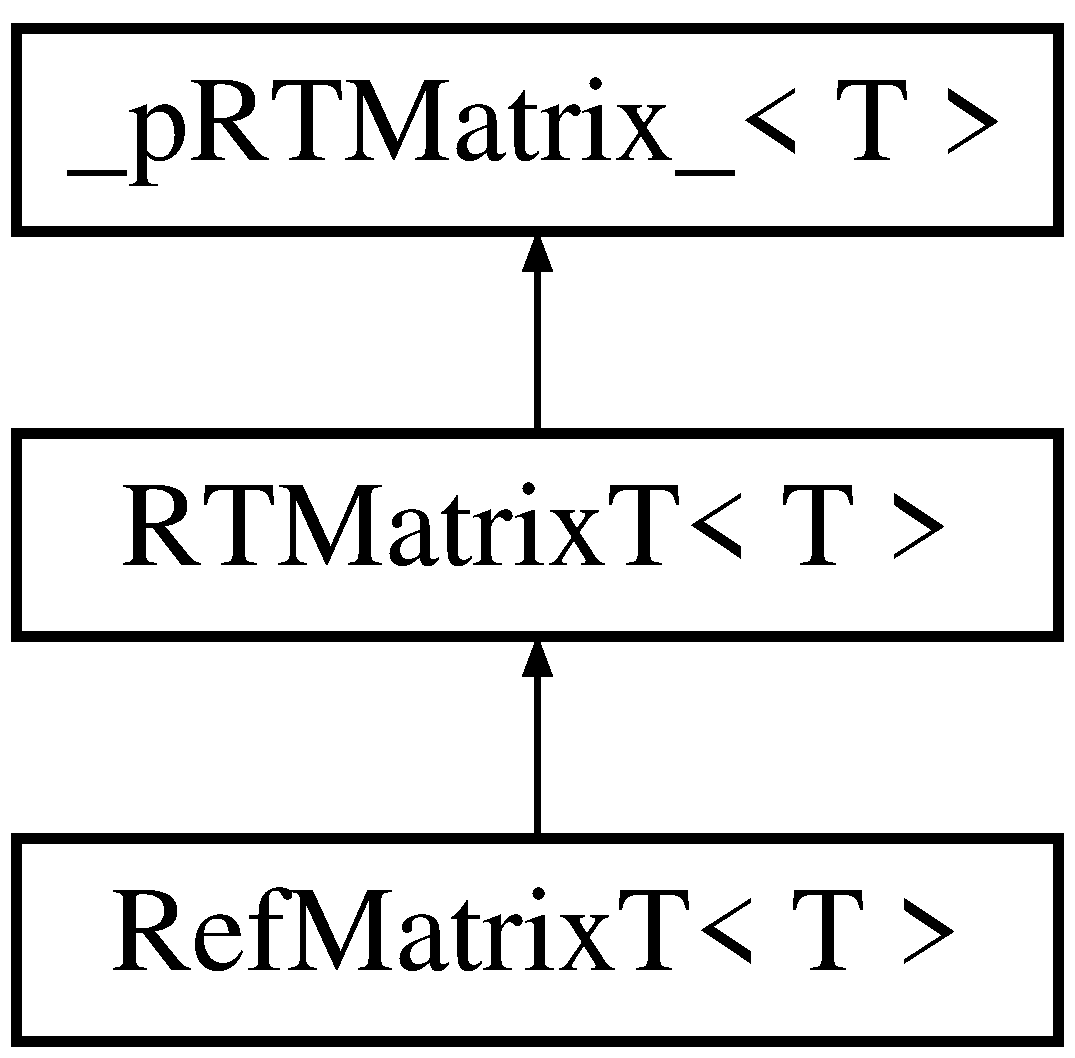
\includegraphics[height=3.000000cm]{classRefMatrixT}
\end{center}
\end{figure}
\subsection*{Public Member Functions}
\begin{DoxyCompactItemize}
\item 
\hypertarget{classRefMatrixT_a8f132026a774d0f19988a35f0869b561}{
{\bfseries RefMatrixT} (uint32 nRows, uint32 nColumns, T $\ast$dataRef)}
\label{classRefMatrixT_a8f132026a774d0f19988a35f0869b561}

\end{DoxyCompactItemize}


\subsection{Detailed Description}
\subsubsection*{template$<$class T$>$class RefMatrixT$<$ T $>$}

a mtrix built on top of a C matrix 

The documentation for this class was generated from the following file:\begin{DoxyCompactItemize}
\item 
\hyperlink{RefMatrix_8h}{RefMatrix.h}\end{DoxyCompactItemize}

\hypertarget{classRTMatrixRow}{
\section{RTMatrixRow$<$ T $>$ Class Template Reference}
\label{classRTMatrixRow}\index{RTMatrixRow@{RTMatrixRow}}
}


{\ttfamily \#include $<$RTMatrix.h$>$}

\subsection*{Public Member Functions}
\begin{DoxyCompactItemize}
\item 
\hyperlink{classRTMatrixRow_a2d2a786e10cca065a792df7c8b1a61d2}{RTMatrixRow} (T $\ast$row)
\item 
T \& \hyperlink{classRTMatrixRow_a20fbed3a18b7984a2155894d741da926}{operator\mbox{[}$\,$\mbox{]}} (int col) const 
\end{DoxyCompactItemize}


\subsection{Detailed Description}
\subsubsection*{template$<$class T$>$class RTMatrixRow$<$ T $>$}

a row of a RTMatrix 

\subsection{Constructor \& Destructor Documentation}
\hypertarget{classRTMatrixRow_a2d2a786e10cca065a792df7c8b1a61d2}{
\index{RTMatrixRow@{RTMatrixRow}!RTMatrixRow@{RTMatrixRow}}
\index{RTMatrixRow@{RTMatrixRow}!RTMatrixRow@{RTMatrixRow}}
\subsubsection[{RTMatrixRow}]{\setlength{\rightskip}{0pt plus 5cm}template$<$class T $>$ {\bf RTMatrixRow}$<$ T $>$::{\bf RTMatrixRow} (
\begin{DoxyParamCaption}
\item[{T $\ast$}]{row}
\end{DoxyParamCaption}
)\hspace{0.3cm}{\ttfamily  \mbox{[}inline\mbox{]}}}}
\label{classRTMatrixRow_a2d2a786e10cca065a792df7c8b1a61d2}
initialise 

\subsection{Member Function Documentation}
\hypertarget{classRTMatrixRow_a20fbed3a18b7984a2155894d741da926}{
\index{RTMatrixRow@{RTMatrixRow}!operator\mbox{[}\mbox{]}@{operator[]}}
\index{operator\mbox{[}\mbox{]}@{operator[]}!RTMatrixRow@{RTMatrixRow}}
\subsubsection[{operator[]}]{\setlength{\rightskip}{0pt plus 5cm}template$<$class T $>$ T\& {\bf RTMatrixRow}$<$ T $>$::operator\mbox{[}$\,$\mbox{]} (
\begin{DoxyParamCaption}
\item[{int}]{col}
\end{DoxyParamCaption}
) const\hspace{0.3cm}{\ttfamily  \mbox{[}inline\mbox{]}}}}
\label{classRTMatrixRow_a20fbed3a18b7984a2155894d741da926}
access the data 

The documentation for this class was generated from the following file:\begin{DoxyCompactItemize}
\item 
\hyperlink{RTMatrix_8h}{RTMatrix.h}\end{DoxyCompactItemize}

\hypertarget{classRTMatrixT}{
\section{RTMatrixT$<$ T $>$ Class Template Reference}
\label{classRTMatrixT}\index{RTMatrixT@{RTMatrixT}}
}


{\ttfamily \#include $<$RTMatrix.h$>$}

Inheritance diagram for RTMatrixT$<$ T $>$:\begin{figure}[H]
\begin{center}
\leavevmode
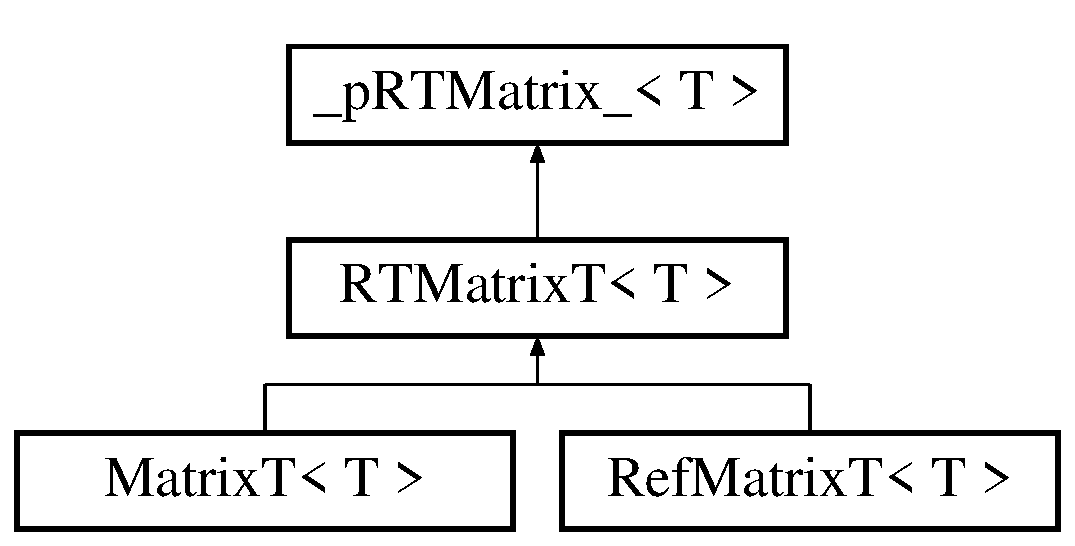
\includegraphics[height=3.000000cm]{classRTMatrixT}
\end{center}
\end{figure}
\subsection*{Public Member Functions}
\begin{DoxyCompactItemize}
\item 
\hypertarget{classRTMatrixT_a4bfc7209460dcb5d9b469d493d8a69ce}{
bool {\bfseries Allocate} (const uint32 nRows, const uint32 nColumns)}
\label{classRTMatrixT_a4bfc7209460dcb5d9b469d493d8a69ce}

\item 
\hypertarget{classRTMatrixT_a59c3e3816d9ad29ad8627e2b3ab649b6}{
void {\bfseries DeAllocate} ()}
\label{classRTMatrixT_a59c3e3816d9ad29ad8627e2b3ab649b6}

\item 
\hypertarget{classRTMatrixT_a4e61750555a3bd0e48514ddeea3dd9bc}{
void {\bfseries Initialize} ()}
\label{classRTMatrixT_a4e61750555a3bd0e48514ddeea3dd9bc}

\item 
\hypertarget{classRTMatrixT_a8925fff21e6a6dac457100cb6eefa345}{
void {\bfseries SwapRows} (uint32 row\_\-i, uint32 row\_\-j)}
\label{classRTMatrixT_a8925fff21e6a6dac457100cb6eefa345}

\item 
\hypertarget{classRTMatrixT_a8bf66bd097cad0600526c8584e2d493f}{
{\bfseries RTMatrixT} (const uint32 nRows, const uint32 nColumns)}
\label{classRTMatrixT_a8bf66bd097cad0600526c8584e2d493f}

\item 
\hypertarget{classRTMatrixT_a84ca2ac42c1c5b945393cf66d83197b0}{
{\bfseries RTMatrixT} (const uint32 nRows, const uint32 nColumns, const T $\ast$source)}
\label{classRTMatrixT_a84ca2ac42c1c5b945393cf66d83197b0}

\item 
\hypertarget{classRTMatrixT_af9e119ed0da618f2730af309f812277f}{
{\bfseries RTMatrixT} (const \hyperlink{classRTMatrixT}{RTMatrixT}$<$ T $>$ \&A)}
\label{classRTMatrixT_af9e119ed0da618f2730af309f812277f}

\item 
\hyperlink{classRTMatrixT_a469d1e9a31a9e81be88464ab444a0a54}{RTMatrixT} (const uint32 nRows, const uint32 nColumns, const char $\ast$options)
\item 
void \hyperlink{classRTMatrixT_ab792ff0825d8c67a79c23b051ee70367}{Zerofy} ()
\item 
void \hyperlink{classRTMatrixT_af16471905a590114f6b560fb14b41350}{Onefy} ()
\item 
void \hyperlink{classRTMatrixT_a2bc71bcbbc5ede802b23620a543f5762}{Eyefy} ()
\item 
void \hyperlink{classRTMatrixT_a1319919a5212715705ff30a4155e1327}{Scale} (const T \&x)
\item 
uint32 \hyperlink{classRTMatrixT_a38179933093473554555dcdfb035e8ce}{NRows} () const 
\item 
uint32 \hyperlink{classRTMatrixT_a2fcc0950e8b0d4c8d00c92aa8a99d59c}{NColumns} () const 
\item 
void \hyperlink{classRTMatrixT_a234c8e2022252db0ff7f9f1a68fb47de}{Clear} ()
\item 
const \hyperlink{classRTMatrixRow}{RTMatrixRow}$<$ T $>$ \hyperlink{classRTMatrixT_afd251c8826e3350e7d2cbdf98a15af2c}{operator\mbox{[}$\,$\mbox{]}} (int rowNo)
\item 
bool \hyperlink{classRTMatrixT_a32bca77e2956ac200c9d8b5b62a93394}{IsNull} ()
\item 
bool \hyperlink{classRTMatrixT_afb183a86036303dba36e56eac881fa38}{Product} (const \hyperlink{classRTMatrixT}{RTMatrixT} \&A, const \hyperlink{classRTMatrixT}{RTMatrixT} \&B)
\item 
bool \hyperlink{classRTMatrixT_ad0ef2110e91e93440f1574567a498419}{DotProduct} (const \hyperlink{classRTMatrixT}{RTMatrixT}$<$ T $>$ \&A)
\item 
bool \hyperlink{classRTMatrixT_af866c8313cb58740b7a4a99665d8aa71}{Sum} (const \hyperlink{classRTMatrixT}{RTMatrixT}$<$ T $>$ \&A, const \hyperlink{classRTMatrixT}{RTMatrixT}$<$ T $>$ \&B)
\item 
bool \hyperlink{classRTMatrixT_a07f4045c3ce877cde806294a336568b2}{Diff} (const \hyperlink{classRTMatrixT}{RTMatrixT}$<$ T $>$ \&A, const \hyperlink{classRTMatrixT}{RTMatrixT}$<$ T $>$ \&B)
\item 
bool \hyperlink{classRTMatrixT_afb66d6eacc34946de4c9470fae15bfcf}{Combine} (const \hyperlink{classRTMatrixT}{RTMatrixT}$<$ T $>$ \&A, const T aw, const \hyperlink{classRTMatrixT}{RTMatrixT}$<$ T $>$ \&B, const T bw)
\item 
T \hyperlink{classRTMatrixT_a42b86d8bf32b5e42292edff8d6e2bc2b}{MaxAbsRowSumNorm} ()
\item 
T \hyperlink{classRTMatrixT_a3a013b9fc461b06dbe2def2eb3318fb5}{MaxAbsColSumNorm} ()
\item 
bool \hyperlink{classRTMatrixT_a16014847a3d1982e3d11ed7ec2b22897}{Transpose} (const \hyperlink{classRTMatrixT}{RTMatrixT}$<$ T $>$ \&A)
\item 
bool \hyperlink{classRTMatrixT_a8b54fe4f49d5b892afa96e54ea4c8e5f}{Invert} (\hyperlink{classRTMatrixT}{RTMatrixT}$<$ T $>$ \&A)
\item 
\hypertarget{classRTMatrixT_a0ea9a7f1df85d8eef54009f607a9b029}{
\hyperlink{classRTMatrixT}{RTMatrixT} \& {\bfseries operator=} (const \hyperlink{classRTMatrixT}{RTMatrixT}$<$ T $>$ \&A)}
\label{classRTMatrixT_a0ea9a7f1df85d8eef54009f607a9b029}

\item 
bool \hyperlink{classRTMatrixT_a76c1f212c944b4de47e556172738cc24}{LU} (\hyperlink{classRTMatrixT}{RTMatrixT}$<$ T $>$ \&L, \hyperlink{classRTMatrixT}{RTMatrixT}$<$ T $>$ \&U, \hyperlink{classRTMatrixT}{RTMatrixT}$<$ T $>$ \&P)
\item 
bool \hyperlink{classRTMatrixT_a9e08c8785510d11b9df86800ca3179a8}{SVD} (\hyperlink{classRTMatrixT}{RTMatrixT}$<$ T $>$ \&U, \hyperlink{classRTMatrixT}{RTMatrixT}$<$ T $>$ \&W, \hyperlink{classRTMatrixT}{RTMatrixT}$<$ T $>$ \&V)
\item 
void \hyperlink{classRTMatrixT_afc165d73e0b9ac3caf53ddf241c73337}{Print} (StreamInterface \&s, int maxrow=10)
\end{DoxyCompactItemize}


\subsection{Detailed Description}
\subsubsection*{template$<$class T$>$class RTMatrixT$<$ T $>$}

The actual RTMatrix 

\subsection{Constructor \& Destructor Documentation}
\hypertarget{classRTMatrixT_a469d1e9a31a9e81be88464ab444a0a54}{
\index{RTMatrixT@{RTMatrixT}!RTMatrixT@{RTMatrixT}}
\index{RTMatrixT@{RTMatrixT}!RTMatrixT@{RTMatrixT}}
\subsubsection[{RTMatrixT}]{\setlength{\rightskip}{0pt plus 5cm}template$<$class T$>$ {\bf RTMatrixT}$<$ T $>$::{\bf RTMatrixT} (
\begin{DoxyParamCaption}
\item[{const uint32}]{nRows, }
\item[{const uint32}]{nColumns, }
\item[{const char $\ast$}]{options}
\end{DoxyParamCaption}
)\hspace{0.3cm}{\ttfamily  \mbox{[}inline\mbox{]}}}}
\label{classRTMatrixT_a469d1e9a31a9e81be88464ab444a0a54}
Constructor for allocating a zeros,ones,eye matrix todo 

\subsection{Member Function Documentation}
\hypertarget{classRTMatrixT_a234c8e2022252db0ff7f9f1a68fb47de}{
\index{RTMatrixT@{RTMatrixT}!Clear@{Clear}}
\index{Clear@{Clear}!RTMatrixT@{RTMatrixT}}
\subsubsection[{Clear}]{\setlength{\rightskip}{0pt plus 5cm}template$<$class T$>$ void {\bf RTMatrixT}$<$ T $>$::Clear (
\begin{DoxyParamCaption}
{}
\end{DoxyParamCaption}
)\hspace{0.3cm}{\ttfamily  \mbox{[}inline\mbox{]}}}}
\label{classRTMatrixT_a234c8e2022252db0ff7f9f1a68fb47de}
Set elements of the matrix to zero. \hypertarget{classRTMatrixT_afb66d6eacc34946de4c9470fae15bfcf}{
\index{RTMatrixT@{RTMatrixT}!Combine@{Combine}}
\index{Combine@{Combine}!RTMatrixT@{RTMatrixT}}
\subsubsection[{Combine}]{\setlength{\rightskip}{0pt plus 5cm}template$<$class T$>$ bool {\bf RTMatrixT}$<$ T $>$::Combine (
\begin{DoxyParamCaption}
\item[{const {\bf RTMatrixT}$<$ T $>$ \&}]{A, }
\item[{const T}]{aw, }
\item[{const {\bf RTMatrixT}$<$ T $>$ \&}]{B, }
\item[{const T}]{bw}
\end{DoxyParamCaption}
)\hspace{0.3cm}{\ttfamily  \mbox{[}inline\mbox{]}}}}
\label{classRTMatrixT_afb66d6eacc34946de4c9470fae15bfcf}
loads the linear combination of A and B WARNING: Uncoherent notation with the parameters in RTM\_\-\_\-vecComb!!! to restabilish eveness maybe is better to change the definition in that functions set. \hypertarget{classRTMatrixT_a07f4045c3ce877cde806294a336568b2}{
\index{RTMatrixT@{RTMatrixT}!Diff@{Diff}}
\index{Diff@{Diff}!RTMatrixT@{RTMatrixT}}
\subsubsection[{Diff}]{\setlength{\rightskip}{0pt plus 5cm}template$<$class T$>$ bool {\bf RTMatrixT}$<$ T $>$::Diff (
\begin{DoxyParamCaption}
\item[{const {\bf RTMatrixT}$<$ T $>$ \&}]{A, }
\item[{const {\bf RTMatrixT}$<$ T $>$ \&}]{B}
\end{DoxyParamCaption}
)\hspace{0.3cm}{\ttfamily  \mbox{[}inline\mbox{]}}}}
\label{classRTMatrixT_a07f4045c3ce877cde806294a336568b2}
loads the difference of A and B \hypertarget{classRTMatrixT_ad0ef2110e91e93440f1574567a498419}{
\index{RTMatrixT@{RTMatrixT}!DotProduct@{DotProduct}}
\index{DotProduct@{DotProduct}!RTMatrixT@{RTMatrixT}}
\subsubsection[{DotProduct}]{\setlength{\rightskip}{0pt plus 5cm}template$<$class T$>$ bool {\bf RTMatrixT}$<$ T $>$::DotProduct (
\begin{DoxyParamCaption}
\item[{const {\bf RTMatrixT}$<$ T $>$ \&}]{A}
\end{DoxyParamCaption}
)\hspace{0.3cm}{\ttfamily  \mbox{[}inline\mbox{]}}}}
\label{classRTMatrixT_ad0ef2110e91e93440f1574567a498419}
this is an element by element product \hypertarget{classRTMatrixT_a2bc71bcbbc5ede802b23620a543f5762}{
\index{RTMatrixT@{RTMatrixT}!Eyefy@{Eyefy}}
\index{Eyefy@{Eyefy}!RTMatrixT@{RTMatrixT}}
\subsubsection[{Eyefy}]{\setlength{\rightskip}{0pt plus 5cm}template$<$class T$>$ void {\bf RTMatrixT}$<$ T $>$::Eyefy (
\begin{DoxyParamCaption}
{}
\end{DoxyParamCaption}
)\hspace{0.3cm}{\ttfamily  \mbox{[}inline\mbox{]}}}}
\label{classRTMatrixT_a2bc71bcbbc5ede802b23620a543f5762}
Set the diagonal entries of the matrix to one, the others to zero. \hypertarget{classRTMatrixT_a8b54fe4f49d5b892afa96e54ea4c8e5f}{
\index{RTMatrixT@{RTMatrixT}!Invert@{Invert}}
\index{Invert@{Invert}!RTMatrixT@{RTMatrixT}}
\subsubsection[{Invert}]{\setlength{\rightskip}{0pt plus 5cm}template$<$class T$>$ bool {\bf RTMatrixT}$<$ T $>$::Invert (
\begin{DoxyParamCaption}
\item[{{\bf RTMatrixT}$<$ T $>$ \&}]{A}
\end{DoxyParamCaption}
)\hspace{0.3cm}{\ttfamily  \mbox{[}inline\mbox{]}}}}
\label{classRTMatrixT_a8b54fe4f49d5b892afa96e54ea4c8e5f}
inverts the matrix A \hypertarget{classRTMatrixT_a32bca77e2956ac200c9d8b5b62a93394}{
\index{RTMatrixT@{RTMatrixT}!IsNull@{IsNull}}
\index{IsNull@{IsNull}!RTMatrixT@{RTMatrixT}}
\subsubsection[{IsNull}]{\setlength{\rightskip}{0pt plus 5cm}template$<$class T$>$ bool {\bf RTMatrixT}$<$ T $>$::IsNull (
\begin{DoxyParamCaption}
{}
\end{DoxyParamCaption}
)\hspace{0.3cm}{\ttfamily  \mbox{[}inline\mbox{]}}}}
\label{classRTMatrixT_a32bca77e2956ac200c9d8b5b62a93394}
Returns True if the matrix is the null one. \hypertarget{classRTMatrixT_a76c1f212c944b4de47e556172738cc24}{
\index{RTMatrixT@{RTMatrixT}!LU@{LU}}
\index{LU@{LU}!RTMatrixT@{RTMatrixT}}
\subsubsection[{LU}]{\setlength{\rightskip}{0pt plus 5cm}template$<$class T$>$ bool {\bf RTMatrixT}$<$ T $>$::LU (
\begin{DoxyParamCaption}
\item[{{\bf RTMatrixT}$<$ T $>$ \&}]{L, }
\item[{{\bf RTMatrixT}$<$ T $>$ \&}]{U, }
\item[{{\bf RTMatrixT}$<$ T $>$ \&}]{P}
\end{DoxyParamCaption}
)\hspace{0.3cm}{\ttfamily  \mbox{[}inline\mbox{]}}}}
\label{classRTMatrixT_a76c1f212c944b4de47e556172738cc24}
LUP Decomposition \hypertarget{classRTMatrixT_a3a013b9fc461b06dbe2def2eb3318fb5}{
\index{RTMatrixT@{RTMatrixT}!MaxAbsColSumNorm@{MaxAbsColSumNorm}}
\index{MaxAbsColSumNorm@{MaxAbsColSumNorm}!RTMatrixT@{RTMatrixT}}
\subsubsection[{MaxAbsColSumNorm}]{\setlength{\rightskip}{0pt plus 5cm}template$<$class T$>$ T {\bf RTMatrixT}$<$ T $>$::MaxAbsColSumNorm (
\begin{DoxyParamCaption}
{}
\end{DoxyParamCaption}
)\hspace{0.3cm}{\ttfamily  \mbox{[}inline\mbox{]}}}}
\label{classRTMatrixT_a3a013b9fc461b06dbe2def2eb3318fb5}
\hypertarget{classRTMatrixT_a42b86d8bf32b5e42292edff8d6e2bc2b}{
\index{RTMatrixT@{RTMatrixT}!MaxAbsRowSumNorm@{MaxAbsRowSumNorm}}
\index{MaxAbsRowSumNorm@{MaxAbsRowSumNorm}!RTMatrixT@{RTMatrixT}}
\subsubsection[{MaxAbsRowSumNorm}]{\setlength{\rightskip}{0pt plus 5cm}template$<$class T$>$ T {\bf RTMatrixT}$<$ T $>$::MaxAbsRowSumNorm (
\begin{DoxyParamCaption}
{}
\end{DoxyParamCaption}
)\hspace{0.3cm}{\ttfamily  \mbox{[}inline\mbox{]}}}}
\label{classRTMatrixT_a42b86d8bf32b5e42292edff8d6e2bc2b}
\hypertarget{classRTMatrixT_a2fcc0950e8b0d4c8d00c92aa8a99d59c}{
\index{RTMatrixT@{RTMatrixT}!NColumns@{NColumns}}
\index{NColumns@{NColumns}!RTMatrixT@{RTMatrixT}}
\subsubsection[{NColumns}]{\setlength{\rightskip}{0pt plus 5cm}template$<$class T$>$ uint32 {\bf RTMatrixT}$<$ T $>$::NColumns (
\begin{DoxyParamCaption}
{}
\end{DoxyParamCaption}
) const\hspace{0.3cm}{\ttfamily  \mbox{[}inline\mbox{]}}}}
\label{classRTMatrixT_a2fcc0950e8b0d4c8d00c92aa8a99d59c}
n of columns \hypertarget{classRTMatrixT_a38179933093473554555dcdfb035e8ce}{
\index{RTMatrixT@{RTMatrixT}!NRows@{NRows}}
\index{NRows@{NRows}!RTMatrixT@{RTMatrixT}}
\subsubsection[{NRows}]{\setlength{\rightskip}{0pt plus 5cm}template$<$class T$>$ uint32 {\bf RTMatrixT}$<$ T $>$::NRows (
\begin{DoxyParamCaption}
{}
\end{DoxyParamCaption}
) const\hspace{0.3cm}{\ttfamily  \mbox{[}inline\mbox{]}}}}
\label{classRTMatrixT_a38179933093473554555dcdfb035e8ce}
n of rows \hypertarget{classRTMatrixT_af16471905a590114f6b560fb14b41350}{
\index{RTMatrixT@{RTMatrixT}!Onefy@{Onefy}}
\index{Onefy@{Onefy}!RTMatrixT@{RTMatrixT}}
\subsubsection[{Onefy}]{\setlength{\rightskip}{0pt plus 5cm}template$<$class T$>$ void {\bf RTMatrixT}$<$ T $>$::Onefy (
\begin{DoxyParamCaption}
{}
\end{DoxyParamCaption}
)\hspace{0.3cm}{\ttfamily  \mbox{[}inline\mbox{]}}}}
\label{classRTMatrixT_af16471905a590114f6b560fb14b41350}
Set elements of the matrix to one. \hypertarget{classRTMatrixT_afd251c8826e3350e7d2cbdf98a15af2c}{
\index{RTMatrixT@{RTMatrixT}!operator\mbox{[}\mbox{]}@{operator[]}}
\index{operator\mbox{[}\mbox{]}@{operator[]}!RTMatrixT@{RTMatrixT}}
\subsubsection[{operator[]}]{\setlength{\rightskip}{0pt plus 5cm}template$<$class T$>$ const {\bf RTMatrixRow}$<$T$>$ {\bf RTMatrixT}$<$ T $>$::operator\mbox{[}$\,$\mbox{]} (
\begin{DoxyParamCaption}
\item[{int}]{rowNo}
\end{DoxyParamCaption}
)\hspace{0.3cm}{\ttfamily  \mbox{[}inline\mbox{]}}}}
\label{classRTMatrixT_afd251c8826e3350e7d2cbdf98a15af2c}
Allow fast access to elements 

Reimplemented in \hyperlink{classMatrixT_a8c84047f97f2d07290a7882884e50397}{MatrixT$<$ T $>$}.

\hypertarget{classRTMatrixT_afc165d73e0b9ac3caf53ddf241c73337}{
\index{RTMatrixT@{RTMatrixT}!Print@{Print}}
\index{Print@{Print}!RTMatrixT@{RTMatrixT}}
\subsubsection[{Print}]{\setlength{\rightskip}{0pt plus 5cm}template$<$class T$>$ void {\bf RTMatrixT}$<$ T $>$::Print (
\begin{DoxyParamCaption}
\item[{StreamInterface \&}]{s, }
\item[{int}]{maxrow = {\ttfamily 10}}
\end{DoxyParamCaption}
)\hspace{0.3cm}{\ttfamily  \mbox{[}inline\mbox{]}}}}
\label{classRTMatrixT_afc165d73e0b9ac3caf53ddf241c73337}
just dumps on stream \hypertarget{classRTMatrixT_afb183a86036303dba36e56eac881fa38}{
\index{RTMatrixT@{RTMatrixT}!Product@{Product}}
\index{Product@{Product}!RTMatrixT@{RTMatrixT}}
\subsubsection[{Product}]{\setlength{\rightskip}{0pt plus 5cm}template$<$class T$>$ bool {\bf RTMatrixT}$<$ T $>$::Product (
\begin{DoxyParamCaption}
\item[{const {\bf RTMatrixT}$<$ T $>$ \&}]{A, }
\item[{const {\bf RTMatrixT}$<$ T $>$ \&}]{B}
\end{DoxyParamCaption}
)\hspace{0.3cm}{\ttfamily  \mbox{[}inline\mbox{]}}}}
\label{classRTMatrixT_afb183a86036303dba36e56eac881fa38}
loads the product of A and B \hypertarget{classRTMatrixT_a1319919a5212715705ff30a4155e1327}{
\index{RTMatrixT@{RTMatrixT}!Scale@{Scale}}
\index{Scale@{Scale}!RTMatrixT@{RTMatrixT}}
\subsubsection[{Scale}]{\setlength{\rightskip}{0pt plus 5cm}template$<$class T$>$ void {\bf RTMatrixT}$<$ T $>$::Scale (
\begin{DoxyParamCaption}
\item[{const T \&}]{x}
\end{DoxyParamCaption}
)\hspace{0.3cm}{\ttfamily  \mbox{[}inline\mbox{]}}}}
\label{classRTMatrixT_a1319919a5212715705ff30a4155e1327}
scale all the values by x \hypertarget{classRTMatrixT_af866c8313cb58740b7a4a99665d8aa71}{
\index{RTMatrixT@{RTMatrixT}!Sum@{Sum}}
\index{Sum@{Sum}!RTMatrixT@{RTMatrixT}}
\subsubsection[{Sum}]{\setlength{\rightskip}{0pt plus 5cm}template$<$class T$>$ bool {\bf RTMatrixT}$<$ T $>$::Sum (
\begin{DoxyParamCaption}
\item[{const {\bf RTMatrixT}$<$ T $>$ \&}]{A, }
\item[{const {\bf RTMatrixT}$<$ T $>$ \&}]{B}
\end{DoxyParamCaption}
)\hspace{0.3cm}{\ttfamily  \mbox{[}inline\mbox{]}}}}
\label{classRTMatrixT_af866c8313cb58740b7a4a99665d8aa71}
loads the sum of A and B \hypertarget{classRTMatrixT_a9e08c8785510d11b9df86800ca3179a8}{
\index{RTMatrixT@{RTMatrixT}!SVD@{SVD}}
\index{SVD@{SVD}!RTMatrixT@{RTMatrixT}}
\subsubsection[{SVD}]{\setlength{\rightskip}{0pt plus 5cm}template$<$class T$>$ bool {\bf RTMatrixT}$<$ T $>$::SVD (
\begin{DoxyParamCaption}
\item[{{\bf RTMatrixT}$<$ T $>$ \&}]{U, }
\item[{{\bf RTMatrixT}$<$ T $>$ \&}]{W, }
\item[{{\bf RTMatrixT}$<$ T $>$ \&}]{V}
\end{DoxyParamCaption}
)\hspace{0.3cm}{\ttfamily  \mbox{[}inline\mbox{]}}}}
\label{classRTMatrixT_a9e08c8785510d11b9df86800ca3179a8}
SVD Decomposition \hypertarget{classRTMatrixT_a16014847a3d1982e3d11ed7ec2b22897}{
\index{RTMatrixT@{RTMatrixT}!Transpose@{Transpose}}
\index{Transpose@{Transpose}!RTMatrixT@{RTMatrixT}}
\subsubsection[{Transpose}]{\setlength{\rightskip}{0pt plus 5cm}template$<$class T$>$ bool {\bf RTMatrixT}$<$ T $>$::Transpose (
\begin{DoxyParamCaption}
\item[{const {\bf RTMatrixT}$<$ T $>$ \&}]{A}
\end{DoxyParamCaption}
)\hspace{0.3cm}{\ttfamily  \mbox{[}inline\mbox{]}}}}
\label{classRTMatrixT_a16014847a3d1982e3d11ed7ec2b22897}
loads the transposed of A \hypertarget{classRTMatrixT_ab792ff0825d8c67a79c23b051ee70367}{
\index{RTMatrixT@{RTMatrixT}!Zerofy@{Zerofy}}
\index{Zerofy@{Zerofy}!RTMatrixT@{RTMatrixT}}
\subsubsection[{Zerofy}]{\setlength{\rightskip}{0pt plus 5cm}template$<$class T$>$ void {\bf RTMatrixT}$<$ T $>$::Zerofy (
\begin{DoxyParamCaption}
{}
\end{DoxyParamCaption}
)\hspace{0.3cm}{\ttfamily  \mbox{[}inline\mbox{]}}}}
\label{classRTMatrixT_ab792ff0825d8c67a79c23b051ee70367}
Set elements of the matrix to zero. 

The documentation for this class was generated from the following file:\begin{DoxyCompactItemize}
\item 
\hyperlink{RTMatrix_8h}{RTMatrix.h}\end{DoxyCompactItemize}

\hypertarget{classSawtoothWaveform}{
\section{SawtoothWaveform Class Reference}
\label{classSawtoothWaveform}\index{SawtoothWaveform@{SawtoothWaveform}}
}
Inheritance diagram for SawtoothWaveform:\begin{figure}[H]
\begin{center}
\leavevmode
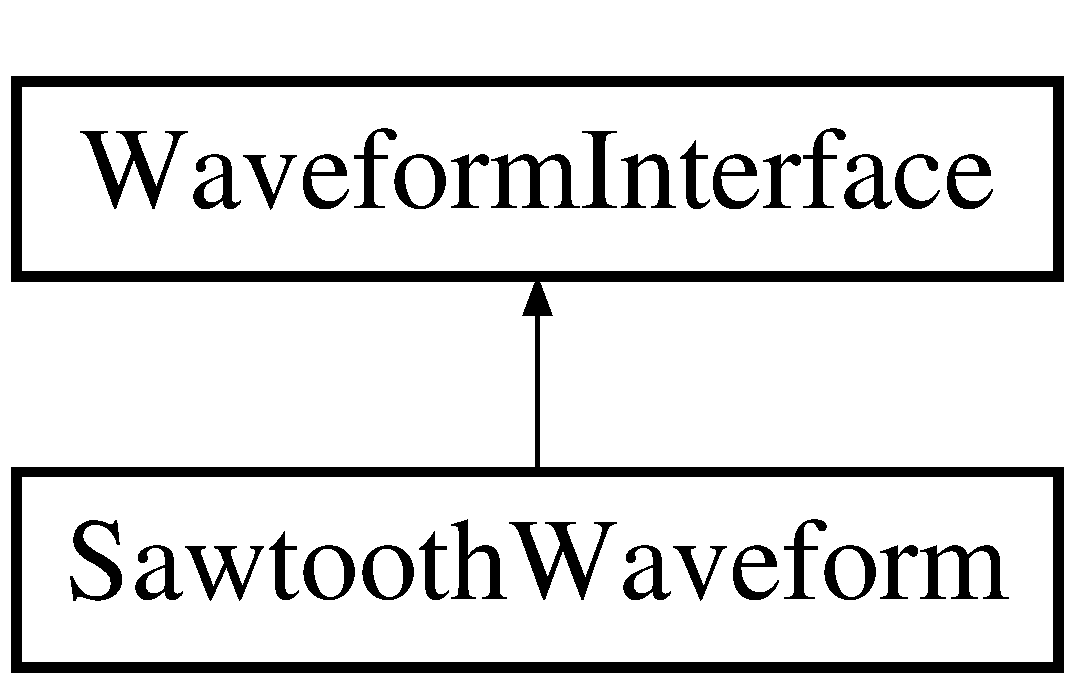
\includegraphics[height=2.000000cm]{classSawtoothWaveform}
\end{center}
\end{figure}
\subsection*{Public Member Functions}
\begin{DoxyCompactItemize}
\item 
\hyperlink{classSawtoothWaveform_a077928022f41def9a00fbb3e7baf4ecf}{SawtoothWaveform} ()
\item 
virtual void \hyperlink{classSawtoothWaveform_a2e5bced67f51dcb46398ce187461ca61}{Reset} ()
\item 
bool \hyperlink{classSawtoothWaveform_a41ffb78c8effe6bf2db7d44194084364}{ObjectLoadSetup} (ConfigurationDataBase \&cdbData, StreamInterface $\ast$err)
\item 
float \hyperlink{classSawtoothWaveform_a9c07e8ba3e7c2e2fc4b8169de7c1684a}{GetValue} (int32 usecTime)
\item 
virtual bool \hyperlink{classSawtoothWaveform_a30516307b4cf8f3c3ef71174e626b739}{ProcessHttpMessage} (HttpStream \&hStream)
\end{DoxyCompactItemize}


\subsection{Constructor \& Destructor Documentation}
\hypertarget{classSawtoothWaveform_a077928022f41def9a00fbb3e7baf4ecf}{
\index{SawtoothWaveform@{SawtoothWaveform}!SawtoothWaveform@{SawtoothWaveform}}
\index{SawtoothWaveform@{SawtoothWaveform}!SawtoothWaveform@{SawtoothWaveform}}
\subsubsection[{SawtoothWaveform}]{\setlength{\rightskip}{0pt plus 5cm}SawtoothWaveform::SawtoothWaveform (
\begin{DoxyParamCaption}
{}
\end{DoxyParamCaption}
)\hspace{0.3cm}{\ttfamily  \mbox{[}inline\mbox{]}}}}
\label{classSawtoothWaveform_a077928022f41def9a00fbb3e7baf4ecf}
Constructor 

\subsection{Member Function Documentation}
\hypertarget{classSawtoothWaveform_a9c07e8ba3e7c2e2fc4b8169de7c1684a}{
\index{SawtoothWaveform@{SawtoothWaveform}!GetValue@{GetValue}}
\index{GetValue@{GetValue}!SawtoothWaveform@{SawtoothWaveform}}
\subsubsection[{GetValue}]{\setlength{\rightskip}{0pt plus 5cm}float SawtoothWaveform::GetValue (
\begin{DoxyParamCaption}
\item[{int32}]{usecTime}
\end{DoxyParamCaption}
)\hspace{0.3cm}{\ttfamily  \mbox{[}inline, virtual\mbox{]}}}}
\label{classSawtoothWaveform_a9c07e8ba3e7c2e2fc4b8169de7c1684a}
Get the current value of the waveform 
\begin{DoxyParams}{Parameters}
{\em usecTime} & current time in microseconds \\
\hline
\end{DoxyParams}
\begin{DoxyReturn}{Returns}
the value of the waveform 
\end{DoxyReturn}


Implements \hyperlink{classWaveformInterface}{WaveformInterface}.

\hypertarget{classSawtoothWaveform_a41ffb78c8effe6bf2db7d44194084364}{
\index{SawtoothWaveform@{SawtoothWaveform}!ObjectLoadSetup@{ObjectLoadSetup}}
\index{ObjectLoadSetup@{ObjectLoadSetup}!SawtoothWaveform@{SawtoothWaveform}}
\subsubsection[{ObjectLoadSetup}]{\setlength{\rightskip}{0pt plus 5cm}bool SawtoothWaveform::ObjectLoadSetup (
\begin{DoxyParamCaption}
\item[{ConfigurationDataBase \&}]{cdbData, }
\item[{StreamInterface $\ast$}]{err}
\end{DoxyParamCaption}
)}}
\label{classSawtoothWaveform_a41ffb78c8effe6bf2db7d44194084364}
Loads object's parameters from a CDB 
\begin{DoxyParams}{Parameters}
{\em cdbData} & the CDB to load configuration from \\
\hline
{\em err} & the StreamInterface to write errors to (not used) \\
\hline
\end{DoxyParams}
\begin{DoxyReturn}{Returns}
True if initialised correctly, False otherwise 
\end{DoxyReturn}
\hypertarget{classSawtoothWaveform_a30516307b4cf8f3c3ef71174e626b739}{
\index{SawtoothWaveform@{SawtoothWaveform}!ProcessHttpMessage@{ProcessHttpMessage}}
\index{ProcessHttpMessage@{ProcessHttpMessage}!SawtoothWaveform@{SawtoothWaveform}}
\subsubsection[{ProcessHttpMessage}]{\setlength{\rightskip}{0pt plus 5cm}bool SawtoothWaveform::ProcessHttpMessage (
\begin{DoxyParamCaption}
\item[{HttpStream \&}]{hStream}
\end{DoxyParamCaption}
)\hspace{0.3cm}{\ttfamily  \mbox{[}virtual\mbox{]}}}}
\label{classSawtoothWaveform_a30516307b4cf8f3c3ef71174e626b739}
Builds a webpage for the current object 
\begin{DoxyParams}{Parameters}
{\em hStream} & the HttpStream to write to \\
\hline
\end{DoxyParams}
\begin{DoxyReturn}{Returns}
True 
\end{DoxyReturn}
\hypertarget{classSawtoothWaveform_a2e5bced67f51dcb46398ce187461ca61}{
\index{SawtoothWaveform@{SawtoothWaveform}!Reset@{Reset}}
\index{Reset@{Reset}!SawtoothWaveform@{SawtoothWaveform}}
\subsubsection[{Reset}]{\setlength{\rightskip}{0pt plus 5cm}virtual void SawtoothWaveform::Reset (
\begin{DoxyParamCaption}
{}
\end{DoxyParamCaption}
)\hspace{0.3cm}{\ttfamily  \mbox{[}inline, virtual\mbox{]}}}}
\label{classSawtoothWaveform_a2e5bced67f51dcb46398ce187461ca61}
Resets the GCNSawtoothWaveform 

Implements \hyperlink{classWaveformInterface}{WaveformInterface}.



The documentation for this class was generated from the following files:\begin{DoxyCompactItemize}
\item 
SawtoothWaveform.h\item 
SawtoothWaveform.cpp\end{DoxyCompactItemize}

\hypertarget{structsColormap}{
\section{sColormap Struct Reference}
\label{structsColormap}\index{sColormap@{sColormap}}
}
\subsection*{Public Attributes}
\begin{DoxyCompactItemize}
\item 
\hypertarget{structsColormap_a20802856b3b681677e1a7dae2a600f26}{
int32 {\bfseries red}}
\label{structsColormap_a20802856b3b681677e1a7dae2a600f26}

\item 
\hypertarget{structsColormap_abcd871229d043dd623922fa65873837c}{
int32 {\bfseries green}}
\label{structsColormap_abcd871229d043dd623922fa65873837c}

\item 
\hypertarget{structsColormap_ac99f9b24b74d39acd2ede6e3b2aaab6f}{
int32 {\bfseries blue}}
\label{structsColormap_ac99f9b24b74d39acd2ede6e3b2aaab6f}

\end{DoxyCompactItemize}


The documentation for this struct was generated from the following file:\begin{DoxyCompactItemize}
\item 
\hyperlink{ColormapInterface_8h}{ColormapInterface.h}\end{DoxyCompactItemize}

\hypertarget{classSequencerWaveform}{
\section{SequencerWaveform Class Reference}
\label{classSequencerWaveform}\index{SequencerWaveform@{SequencerWaveform}}
}
Inheritance diagram for SequencerWaveform:\begin{figure}[H]
\begin{center}
\leavevmode
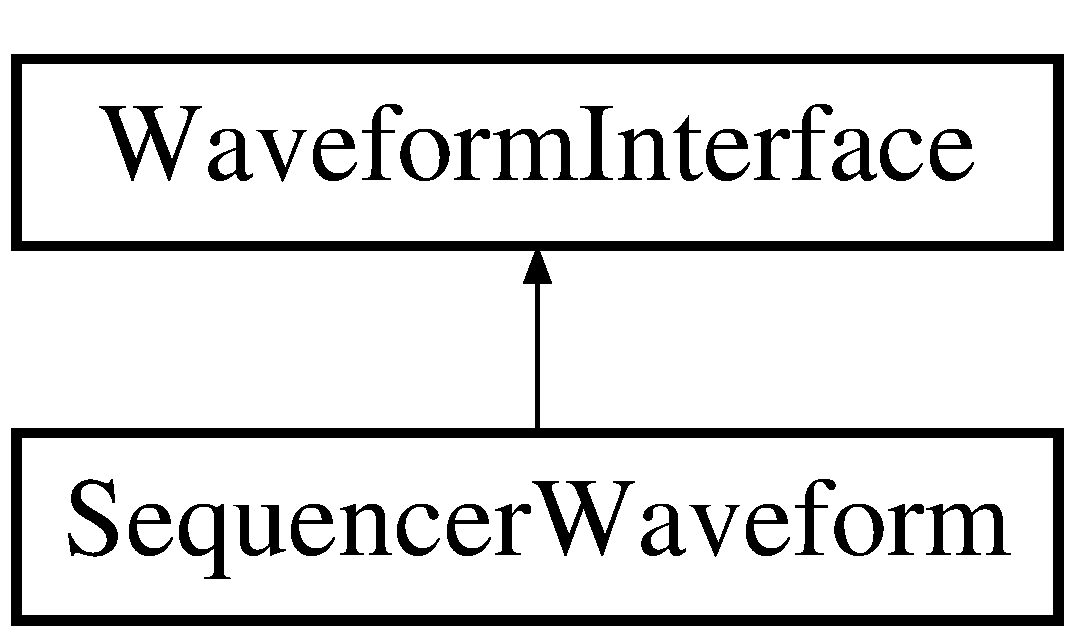
\includegraphics[height=2.000000cm]{classSequencerWaveform}
\end{center}
\end{figure}
\subsection*{Public Member Functions}
\begin{DoxyCompactItemize}
\item 
\hypertarget{classSequencerWaveform_a5e0baeafd599b64460e85cec2320155d}{
virtual void {\bfseries Reset} ()}
\label{classSequencerWaveform_a5e0baeafd599b64460e85cec2320155d}

\item 
virtual bool \hyperlink{classSequencerWaveform_a866ae8324e1e035eac1d99ca73efd587}{ObjectLoadSetup} (ConfigurationDataBase \&cdbData, StreamInterface $\ast$err)
\item 
virtual bool \hyperlink{classSequencerWaveform_a72ad2420ff153ff20d66399a2a59dbc6}{ProcessHttpMessage} (HttpStream \&hStream)
\item 
\hypertarget{classSequencerWaveform_a70e5009fba42d9fde521879ecfbcf5c8}{
virtual float {\bfseries GetValue} (int32 usecTime)}
\label{classSequencerWaveform_a70e5009fba42d9fde521879ecfbcf5c8}

\end{DoxyCompactItemize}


\subsection{Member Function Documentation}
\hypertarget{classSequencerWaveform_a866ae8324e1e035eac1d99ca73efd587}{
\index{SequencerWaveform@{SequencerWaveform}!ObjectLoadSetup@{ObjectLoadSetup}}
\index{ObjectLoadSetup@{ObjectLoadSetup}!SequencerWaveform@{SequencerWaveform}}
\subsubsection[{ObjectLoadSetup}]{\setlength{\rightskip}{0pt plus 5cm}bool SequencerWaveform::ObjectLoadSetup (
\begin{DoxyParamCaption}
\item[{ConfigurationDataBase \&}]{cdbData, }
\item[{StreamInterface $\ast$}]{err}
\end{DoxyParamCaption}
)\hspace{0.3cm}{\ttfamily  \mbox{[}virtual\mbox{]}}}}
\label{classSequencerWaveform_a866ae8324e1e035eac1d99ca73efd587}
Loads parameters from a CDB 
\begin{DoxyParams}{Parameters}
{\em cdbData} & the CDB \\
\hline
\end{DoxyParams}
\begin{DoxyReturn}{Returns}
True if the initialisation went ok, False otherwise 
\end{DoxyReturn}
\hypertarget{classSequencerWaveform_a72ad2420ff153ff20d66399a2a59dbc6}{
\index{SequencerWaveform@{SequencerWaveform}!ProcessHttpMessage@{ProcessHttpMessage}}
\index{ProcessHttpMessage@{ProcessHttpMessage}!SequencerWaveform@{SequencerWaveform}}
\subsubsection[{ProcessHttpMessage}]{\setlength{\rightskip}{0pt plus 5cm}bool SequencerWaveform::ProcessHttpMessage (
\begin{DoxyParamCaption}
\item[{HttpStream \&}]{hStream}
\end{DoxyParamCaption}
)\hspace{0.3cm}{\ttfamily  \mbox{[}virtual\mbox{]}}}}
\label{classSequencerWaveform_a72ad2420ff153ff20d66399a2a59dbc6}
Builds a webpage for the current object 
\begin{DoxyParams}{Parameters}
{\em hStream} & the HttpStream to write to \\
\hline
\end{DoxyParams}
\begin{DoxyReturn}{Returns}
True 
\end{DoxyReturn}


The documentation for this class was generated from the following files:\begin{DoxyCompactItemize}
\item 
SequencerWaveform.h\item 
SequencerWaveform.cpp\end{DoxyCompactItemize}

\hypertarget{classSignalArchiver}{
\section{SignalArchiver Class Reference}
\label{classSignalArchiver}\index{SignalArchiver@{SignalArchiver}}
}
Inheritance diagram for SignalArchiver:\begin{figure}[H]
\begin{center}
\leavevmode
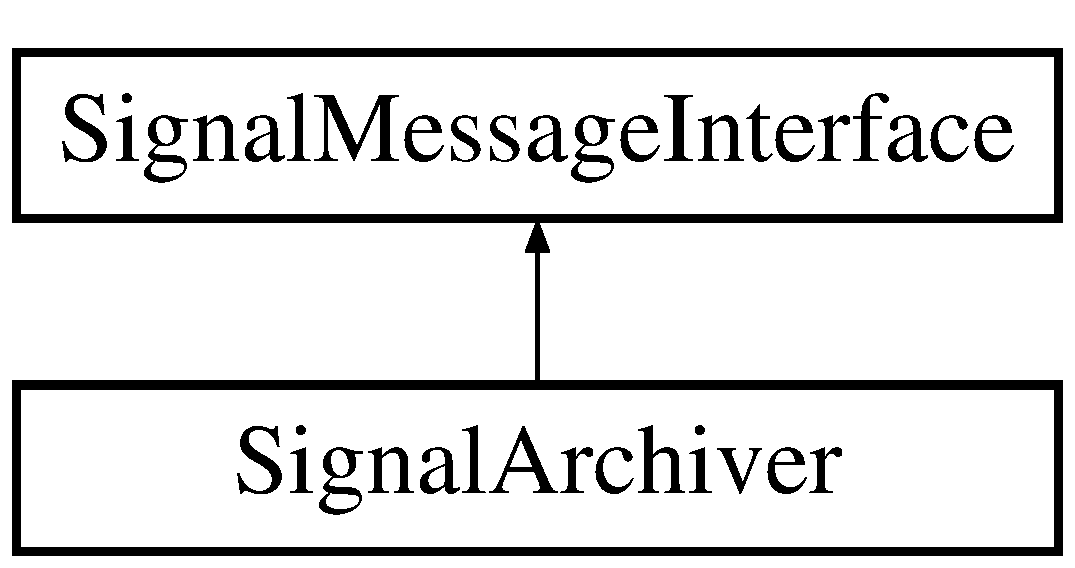
\includegraphics[height=2.000000cm]{classSignalArchiver}
\end{center}
\end{figure}
\subsection*{Public Member Functions}
\begin{DoxyCompactItemize}
\item 
virtual \hyperlink{classSignalArchiver_a68e2febb702e5ef39599b2e4a7934169}{$\sim$SignalArchiver} ()
\item 
\hyperlink{classSignalArchiver_adf6593128ebb50107f6861096702cc35}{SignalArchiver} ()
\item 
virtual bool \hyperlink{classSignalArchiver_a149116390dd9f9e511c4704480a48352}{ProcessHttpMessage} (HttpStream \&hStream)
\item 
\hypertarget{classSignalArchiver_a6b33d4d213c862228a60140de0d72a30}{
virtual bool {\bfseries ObjectLoadSetup} (ConfigurationDataBase \&info, StreamInterface $\ast$err)}
\label{classSignalArchiver_a6b33d4d213c862228a60140de0d72a30}

\item 
virtual bool \hyperlink{classSignalArchiver_a09622d82d9e4a388bd26d75353a10d98}{ProcessMessage} (GCRTemplate$<$ MessageEnvelope $>$ envelope)
\end{DoxyCompactItemize}
\subsection*{Friends}
\begin{DoxyCompactItemize}
\item 
void \hyperlink{classSignalArchiver_ab48b650b85581a0ea28f252b1650bf8b}{SignalArchivingFn} (void $\ast$args)
\end{DoxyCompactItemize}


\subsection{Constructor \& Destructor Documentation}
\hypertarget{classSignalArchiver_a68e2febb702e5ef39599b2e4a7934169}{
\index{SignalArchiver@{SignalArchiver}!$\sim$SignalArchiver@{$\sim$SignalArchiver}}
\index{$\sim$SignalArchiver@{$\sim$SignalArchiver}!SignalArchiver@{SignalArchiver}}
\subsubsection[{$\sim$SignalArchiver}]{\setlength{\rightskip}{0pt plus 5cm}virtual SignalArchiver::$\sim$SignalArchiver (
\begin{DoxyParamCaption}
{}
\end{DoxyParamCaption}
)\hspace{0.3cm}{\ttfamily  \mbox{[}inline, virtual\mbox{]}}}}
\label{classSignalArchiver_a68e2febb702e5ef39599b2e4a7934169}
\hypertarget{classSignalArchiver_adf6593128ebb50107f6861096702cc35}{
\index{SignalArchiver@{SignalArchiver}!SignalArchiver@{SignalArchiver}}
\index{SignalArchiver@{SignalArchiver}!SignalArchiver@{SignalArchiver}}
\subsubsection[{SignalArchiver}]{\setlength{\rightskip}{0pt plus 5cm}SignalArchiver::SignalArchiver (
\begin{DoxyParamCaption}
{}
\end{DoxyParamCaption}
)\hspace{0.3cm}{\ttfamily  \mbox{[}inline\mbox{]}}}}
\label{classSignalArchiver_adf6593128ebb50107f6861096702cc35}


\subsection{Member Function Documentation}
\hypertarget{classSignalArchiver_a149116390dd9f9e511c4704480a48352}{
\index{SignalArchiver@{SignalArchiver}!ProcessHttpMessage@{ProcessHttpMessage}}
\index{ProcessHttpMessage@{ProcessHttpMessage}!SignalArchiver@{SignalArchiver}}
\subsubsection[{ProcessHttpMessage}]{\setlength{\rightskip}{0pt plus 5cm}virtual bool SignalArchiver::ProcessHttpMessage (
\begin{DoxyParamCaption}
\item[{HttpStream \&}]{hStream}
\end{DoxyParamCaption}
)\hspace{0.3cm}{\ttfamily  \mbox{[}inline, virtual\mbox{]}}}}
\label{classSignalArchiver_a149116390dd9f9e511c4704480a48352}
The HTTP entry point (it is delegated to an HttpDirectoryResource \hypertarget{classSignalArchiver_a09622d82d9e4a388bd26d75353a10d98}{
\index{SignalArchiver@{SignalArchiver}!ProcessMessage@{ProcessMessage}}
\index{ProcessMessage@{ProcessMessage}!SignalArchiver@{SignalArchiver}}
\subsubsection[{ProcessMessage}]{\setlength{\rightskip}{0pt plus 5cm}virtual bool SignalArchiver::ProcessMessage (
\begin{DoxyParamCaption}
\item[{GCRTemplate$<$ MessageEnvelope $>$}]{envelope}
\end{DoxyParamCaption}
)\hspace{0.3cm}{\ttfamily  \mbox{[}inline, virtual\mbox{]}}}}
\label{classSignalArchiver_a09622d82d9e4a388bd26d75353a10d98}
Processes the incoming message and checks for the content. If the code is relativeDirectoryPathMessageCode then it will set the relativeDirectoryPath = to the message content If the content is STORESIGNALS, data storage is triggered, otherwise \hyperlink{classSignalMessageInterface_ae9f04a9f88929ffc4b9761a41d13cec7}{SignalMessageInterface::ProcessMessage} is called 

Reimplemented from \hyperlink{classSignalMessageInterface_ae9f04a9f88929ffc4b9761a41d13cec7}{SignalMessageInterface}.



\subsection{Friends And Related Function Documentation}
\hypertarget{classSignalArchiver_ab48b650b85581a0ea28f252b1650bf8b}{
\index{SignalArchiver@{SignalArchiver}!SignalArchivingFn@{SignalArchivingFn}}
\index{SignalArchivingFn@{SignalArchivingFn}!SignalArchiver@{SignalArchiver}}
\subsubsection[{SignalArchivingFn}]{\setlength{\rightskip}{0pt plus 5cm}void SignalArchivingFn (
\begin{DoxyParamCaption}
\item[{void $\ast$}]{args}
\end{DoxyParamCaption}
)\hspace{0.3cm}{\ttfamily  \mbox{[}friend\mbox{]}}}}
\label{classSignalArchiver_ab48b650b85581a0ea28f252b1650bf8b}
Thread which stores the signals, to avoid blocking the messaging mechanism 

The documentation for this class was generated from the following files:\begin{DoxyCompactItemize}
\item 
SignalArchiver.h\item 
SignalArchiver.cpp\end{DoxyCompactItemize}

\hypertarget{classSignalLister}{
\section{SignalLister Class Reference}
\label{classSignalLister}\index{SignalLister@{SignalLister}}
}
\subsection*{Public Member Functions}
\begin{DoxyCompactItemize}
\item 
\hyperlink{classSignalLister_af86dfcbd029baf630223264e2d573a82}{SignalLister} (\hyperlink{classSignalMessageInterface}{SignalMessageInterface} $\ast$source=NULL)
\item 
virtual void \hyperlink{classSignalLister_a2153a04a561f195558985824a0f16000}{Do} (GCReference data)
\item 
virtual void \hyperlink{classSignalLister_ae07d72d9481f44c5fb071f901ded11fb}{Do2} (GCReference data, SFTestType mode)
\end{DoxyCompactItemize}


\subsection{Detailed Description}
Send message to all objects of a given criteria 

\subsection{Constructor \& Destructor Documentation}
\hypertarget{classSignalLister_af86dfcbd029baf630223264e2d573a82}{
\index{SignalLister@{SignalLister}!SignalLister@{SignalLister}}
\index{SignalLister@{SignalLister}!SignalLister@{SignalLister}}
\subsubsection[{SignalLister}]{\setlength{\rightskip}{0pt plus 5cm}SignalLister::SignalLister (
\begin{DoxyParamCaption}
\item[{{\bf SignalMessageInterface} $\ast$}]{source = {\ttfamily NULL}}
\end{DoxyParamCaption}
)\hspace{0.3cm}{\ttfamily  \mbox{[}inline\mbox{]}}}}
\label{classSignalLister_af86dfcbd029baf630223264e2d573a82}


\subsection{Member Function Documentation}
\hypertarget{classSignalLister_a2153a04a561f195558985824a0f16000}{
\index{SignalLister@{SignalLister}!Do@{Do}}
\index{Do@{Do}!SignalLister@{SignalLister}}
\subsubsection[{Do}]{\setlength{\rightskip}{0pt plus 5cm}virtual void SignalLister::Do (
\begin{DoxyParamCaption}
\item[{GCReference}]{data}
\end{DoxyParamCaption}
)\hspace{0.3cm}{\ttfamily  \mbox{[}inline, virtual\mbox{]}}}}
\label{classSignalLister_a2153a04a561f195558985824a0f16000}
actual function \hypertarget{classSignalLister_ae07d72d9481f44c5fb071f901ded11fb}{
\index{SignalLister@{SignalLister}!Do2@{Do2}}
\index{Do2@{Do2}!SignalLister@{SignalLister}}
\subsubsection[{Do2}]{\setlength{\rightskip}{0pt plus 5cm}virtual void SignalLister::Do2 (
\begin{DoxyParamCaption}
\item[{GCReference}]{data, }
\item[{SFTestType}]{mode}
\end{DoxyParamCaption}
)\hspace{0.3cm}{\ttfamily  \mbox{[}inline, virtual\mbox{]}}}}
\label{classSignalLister_ae07d72d9481f44c5fb071f901ded11fb}
actual function 

The documentation for this class was generated from the following file:\begin{DoxyCompactItemize}
\item 
SignalMessageInterface.cpp\end{DoxyCompactItemize}

\hypertarget{classSignalMessageInterface}{
\section{SignalMessageInterface Class Reference}
\label{classSignalMessageInterface}\index{SignalMessageInterface@{SignalMessageInterface}}
}
Inheritance diagram for SignalMessageInterface:\begin{figure}[H]
\begin{center}
\leavevmode
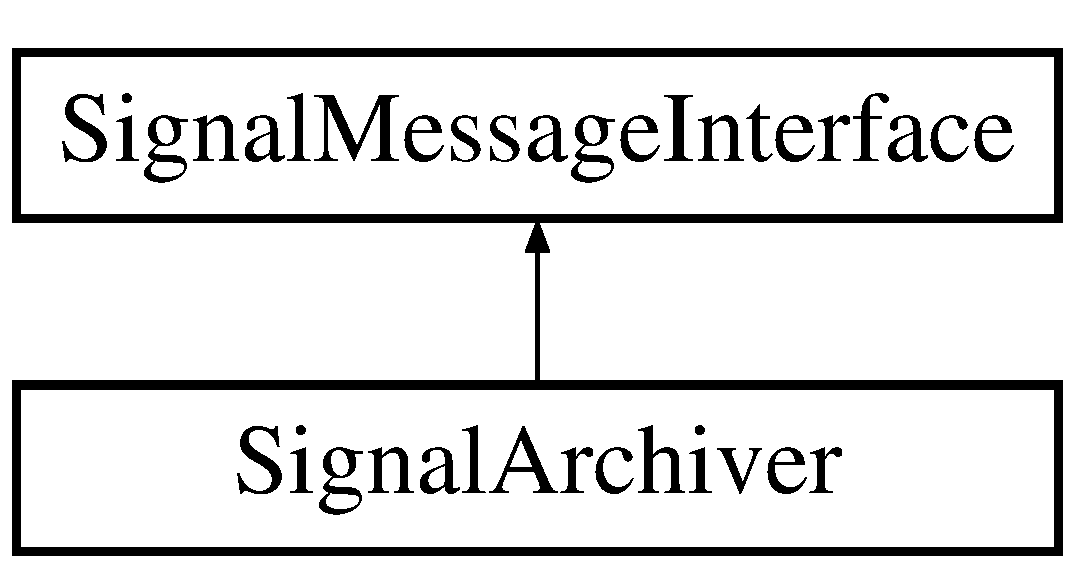
\includegraphics[height=2.000000cm]{classSignalMessageInterface}
\end{center}
\end{figure}
\subsection*{Public Member Functions}
\begin{DoxyCompactItemize}
\item 
\hypertarget{classSignalMessageInterface_ad30c68bf40274ca07f78f2a282ecd9c3}{
virtual bool {\bfseries ObjectLoadSetup} (ConfigurationDataBase \&info, StreamInterface $\ast$err)}
\label{classSignalMessageInterface_ad30c68bf40274ca07f78f2a282ecd9c3}

\item 
virtual bool \hyperlink{classSignalMessageInterface_ae9f04a9f88929ffc4b9761a41d13cec7}{ProcessMessage} (GCRTemplate$<$ MessageEnvelope $>$ envelope)
\end{DoxyCompactItemize}
\subsection*{Protected Member Functions}
\begin{DoxyCompactItemize}
\item 
GCRTemplate$<$ SignalInterface $>$ \hyperlink{classSignalMessageInterface_a9ae57567143070dd72e8789d7ba02ab1}{GetSignal} (const char $\ast$signalName)
\item 
void \hyperlink{classSignalMessageInterface_a9236f714b5eb1164637662c4eb607e98}{RemoveIllegalCharacters} (FString \&toBuild, FString \&signalName, const char $\ast$illegalCharacters)
\end{DoxyCompactItemize}
\subsection*{Protected Attributes}
\begin{DoxyCompactItemize}
\item 
ConfigurationDataBase \hyperlink{classSignalMessageInterface_a4444ccf4557431cbd475af82a8131d58}{signalDataBase}
\end{DoxyCompactItemize}
\subsection*{Friends}
\begin{DoxyCompactItemize}
\item 
GCRTemplate$<$ SignalInterface $>$ \hyperlink{classSignalMessageInterface_a5ac0c04a16d02b3b32e4657030fc37a7}{SMIGetSignal} (\hyperlink{classSignalMessageInterface}{SignalMessageInterface} \&smi, const char $\ast$signalName)
\item 
bool \hyperlink{classSignalMessageInterface_ace687065e8ad1504bbfa067e025560b9}{SMIProcessMessage} (\hyperlink{classSignalMessageInterface}{SignalMessageInterface} \&smi, GCRTemplate$<$ MessageEnvelope $>$ envelope)
\end{DoxyCompactItemize}


\subsection{Member Function Documentation}
\hypertarget{classSignalMessageInterface_a9ae57567143070dd72e8789d7ba02ab1}{
\index{SignalMessageInterface@{SignalMessageInterface}!GetSignal@{GetSignal}}
\index{GetSignal@{GetSignal}!SignalMessageInterface@{SignalMessageInterface}}
\subsubsection[{GetSignal}]{\setlength{\rightskip}{0pt plus 5cm}GCRTemplate$<$SignalInterface$>$ SignalMessageInterface::GetSignal (
\begin{DoxyParamCaption}
\item[{const char $\ast$}]{signalName}
\end{DoxyParamCaption}
)\hspace{0.3cm}{\ttfamily  \mbox{[}inline, protected\mbox{]}}}}
\label{classSignalMessageInterface_a9ae57567143070dd72e8789d7ba02ab1}
\begin{DoxySeeAlso}{See also}
\hyperlink{classSignalMessageInterface_a5ac0c04a16d02b3b32e4657030fc37a7}{SMIGetSignal} 
\end{DoxySeeAlso}
\hypertarget{classSignalMessageInterface_ae9f04a9f88929ffc4b9761a41d13cec7}{
\index{SignalMessageInterface@{SignalMessageInterface}!ProcessMessage@{ProcessMessage}}
\index{ProcessMessage@{ProcessMessage}!SignalMessageInterface@{SignalMessageInterface}}
\subsubsection[{ProcessMessage}]{\setlength{\rightskip}{0pt plus 5cm}virtual bool SignalMessageInterface::ProcessMessage (
\begin{DoxyParamCaption}
\item[{GCRTemplate$<$ MessageEnvelope $>$}]{envelope}
\end{DoxyParamCaption}
)\hspace{0.3cm}{\ttfamily  \mbox{[}inline, virtual\mbox{]}}}}
\label{classSignalMessageInterface_ae9f04a9f88929ffc4b9761a41d13cec7}
This interface operates on Messages with code 0 The meaningful contents are AUTODETECT it first wipes the list of signal searches for GAMS with MessageHandlerInterface that reply to the question LISTSIGNALS with a user message ADDSIGNAL containing a number of GCNString objects (one for each signal) The object name should match the signal name.... The string should contain the name of the signal the type and size This is a processed version of the signalName Any non CDB valid character are replaced by \#XX wher XX is the hex Name = SIGNALNAME\par
 DataType=TYPE\par
 MaxSize=SIZE\par
 Dimensions= \{ d1 d2 ... \} // opzionale (This is a CDB compatible format) TYPE is the string rapresentation of the BasicType SIZE is the max number of object that will be returned This information is then converted in CDB format and stored in the signalDataBase 

Reimplemented in \hyperlink{classSignalArchiver_a09622d82d9e4a388bd26d75353a10d98}{SignalArchiver}.

\hypertarget{classSignalMessageInterface_a9236f714b5eb1164637662c4eb607e98}{
\index{SignalMessageInterface@{SignalMessageInterface}!RemoveIllegalCharacters@{RemoveIllegalCharacters}}
\index{RemoveIllegalCharacters@{RemoveIllegalCharacters}!SignalMessageInterface@{SignalMessageInterface}}
\subsubsection[{RemoveIllegalCharacters}]{\setlength{\rightskip}{0pt plus 5cm}void SignalMessageInterface::RemoveIllegalCharacters (
\begin{DoxyParamCaption}
\item[{FString \&}]{toBuild, }
\item[{FString \&}]{signalName, }
\item[{const char $\ast$}]{illegalCharacters}
\end{DoxyParamCaption}
)\hspace{0.3cm}{\ttfamily  \mbox{[}inline, protected\mbox{]}}}}
\label{classSignalMessageInterface_a9236f714b5eb1164637662c4eb607e98}
Removes illegal characters from signal names 
\begin{DoxyParams}{Parameters}
{\em toBuild} & an FString without the illegal characters \\
\hline
{\em signalName} & the original signal name \\
\hline
{\em illegalCharacters} & the characters to be removed \\
\hline
\end{DoxyParams}


\subsection{Friends And Related Function Documentation}
\hypertarget{classSignalMessageInterface_a5ac0c04a16d02b3b32e4657030fc37a7}{
\index{SignalMessageInterface@{SignalMessageInterface}!SMIGetSignal@{SMIGetSignal}}
\index{SMIGetSignal@{SMIGetSignal}!SignalMessageInterface@{SignalMessageInterface}}
\subsubsection[{SMIGetSignal}]{\setlength{\rightskip}{0pt plus 5cm}GCRTemplate$<$SignalInterface$>$ SMIGetSignal (
\begin{DoxyParamCaption}
\item[{{\bf SignalMessageInterface} \&}]{smi, }
\item[{const char $\ast$}]{signalName}
\end{DoxyParamCaption}
)\hspace{0.3cm}{\ttfamily  \mbox{[}friend\mbox{]}}}}
\label{classSignalMessageInterface_a5ac0c04a16d02b3b32e4657030fc37a7}
C function definitions retrieves from cache or from the collectors 
\begin{DoxyParams}{Parameters}
{\em smi} & the \hyperlink{classSignalMessageInterface}{SignalMessageInterface} object \\
\hline
{\em signalName} & the signal name as returned by the listing AUTODETECT method \\
\hline
\end{DoxyParams}
\begin{DoxyReturn}{Returns}
the signal data 
\end{DoxyReturn}
\hypertarget{classSignalMessageInterface_ace687065e8ad1504bbfa067e025560b9}{
\index{SignalMessageInterface@{SignalMessageInterface}!SMIProcessMessage@{SMIProcessMessage}}
\index{SMIProcessMessage@{SMIProcessMessage}!SignalMessageInterface@{SignalMessageInterface}}
\subsubsection[{SMIProcessMessage}]{\setlength{\rightskip}{0pt plus 5cm}bool SMIProcessMessage (
\begin{DoxyParamCaption}
\item[{{\bf SignalMessageInterface} \&}]{smi, }
\item[{GCRTemplate$<$ MessageEnvelope $>$}]{envelope}
\end{DoxyParamCaption}
)\hspace{0.3cm}{\ttfamily  \mbox{[}friend\mbox{]}}}}
\label{classSignalMessageInterface_ace687065e8ad1504bbfa067e025560b9}
Handles the message requests

\begin{DoxySeeAlso}{See also}
\hyperlink{classSignalMessageInterface_ae9f04a9f88929ffc4b9761a41d13cec7}{SignalMessageInterface::ProcessMessage} 
\end{DoxySeeAlso}


\subsection{Member Data Documentation}
\hypertarget{classSignalMessageInterface_a4444ccf4557431cbd475af82a8131d58}{
\index{SignalMessageInterface@{SignalMessageInterface}!signalDataBase@{signalDataBase}}
\index{signalDataBase@{signalDataBase}!SignalMessageInterface@{SignalMessageInterface}}
\subsubsection[{signalDataBase}]{\setlength{\rightskip}{0pt plus 5cm}ConfigurationDataBase {\bf SignalMessageInterface::signalDataBase}\hspace{0.3cm}{\ttfamily  \mbox{[}protected\mbox{]}}}}
\label{classSignalMessageInterface_a4444ccf4557431cbd475af82a8131d58}
The database with the signals 

The documentation for this class was generated from the following file:\begin{DoxyCompactItemize}
\item 
SignalMessageInterface.h\end{DoxyCompactItemize}

\hypertarget{classsimple}{
\section{simple Class Reference}
\label{classsimple}\index{simple@{simple}}
}


The documentation for this class was generated from the following file:\begin{DoxyCompactItemize}
\item 
ObjectBrowserMenu.cpp\end{DoxyCompactItemize}

\hypertarget{classSineWaveform}{
\section{SineWaveform Class Reference}
\label{classSineWaveform}\index{SineWaveform@{SineWaveform}}
}
Inheritance diagram for SineWaveform:\begin{figure}[H]
\begin{center}
\leavevmode
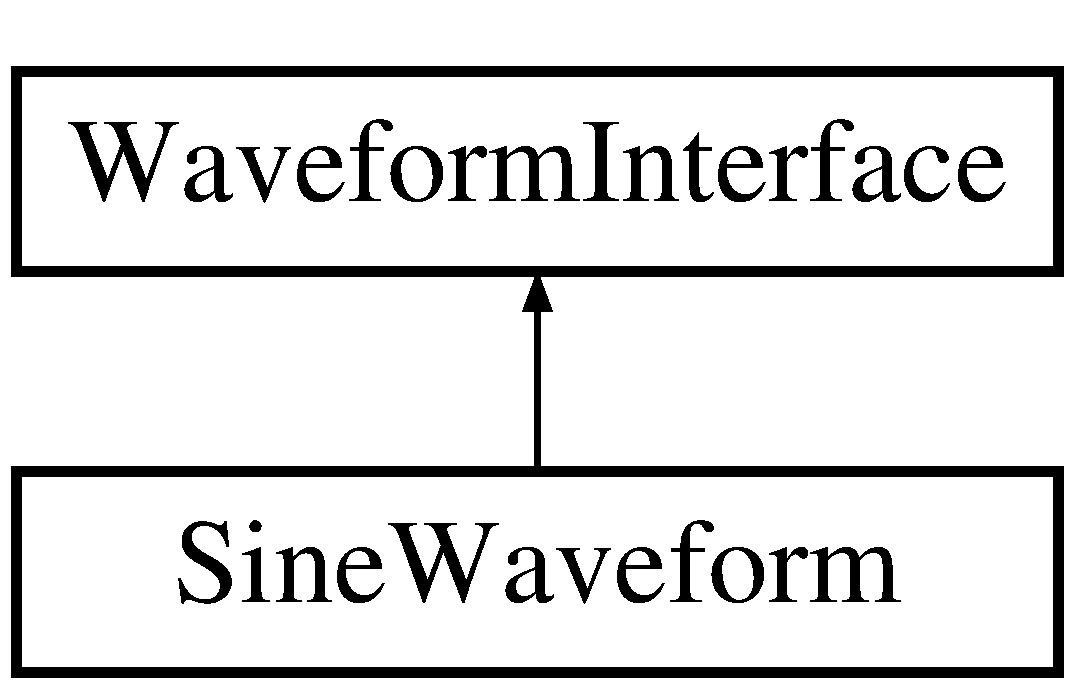
\includegraphics[height=2.000000cm]{classSineWaveform}
\end{center}
\end{figure}
\subsection*{Public Member Functions}
\begin{DoxyCompactItemize}
\item 
\hypertarget{classSineWaveform_a9dbdb5198162d1eb402c4fc0f65f5c8e}{
virtual void {\bfseries Reset} ()}
\label{classSineWaveform_a9dbdb5198162d1eb402c4fc0f65f5c8e}

\item 
virtual bool \hyperlink{classSineWaveform_aed05eed95ba2325d32f68523dfa815e9}{ObjectLoadSetup} (ConfigurationDataBase \&cdbData, StreamInterface $\ast$err)
\item 
virtual bool \hyperlink{classSineWaveform_a98a9876eedef78a3f4ac1fe2cc5aa1bd}{ProcessHttpMessage} (HttpStream \&hStream)
\item 
\hypertarget{classSineWaveform_a919252ac1127ee2bb0c0e2138d32402a}{
virtual float {\bfseries GetValue} (int32 usecTime)}
\label{classSineWaveform_a919252ac1127ee2bb0c0e2138d32402a}

\end{DoxyCompactItemize}


\subsection{Member Function Documentation}
\hypertarget{classSineWaveform_aed05eed95ba2325d32f68523dfa815e9}{
\index{SineWaveform@{SineWaveform}!ObjectLoadSetup@{ObjectLoadSetup}}
\index{ObjectLoadSetup@{ObjectLoadSetup}!SineWaveform@{SineWaveform}}
\subsubsection[{ObjectLoadSetup}]{\setlength{\rightskip}{0pt plus 5cm}bool SineWaveform::ObjectLoadSetup (
\begin{DoxyParamCaption}
\item[{ConfigurationDataBase \&}]{cdbData, }
\item[{StreamInterface $\ast$}]{err}
\end{DoxyParamCaption}
)\hspace{0.3cm}{\ttfamily  \mbox{[}virtual\mbox{]}}}}
\label{classSineWaveform_aed05eed95ba2325d32f68523dfa815e9}
Loads parameters from a CDB 
\begin{DoxyParams}{Parameters}
{\em cdbData} & the CDB \\
\hline
\end{DoxyParams}
\begin{DoxyReturn}{Returns}
True if the initialisation went ok, False otherwise 
\end{DoxyReturn}
\hypertarget{classSineWaveform_a98a9876eedef78a3f4ac1fe2cc5aa1bd}{
\index{SineWaveform@{SineWaveform}!ProcessHttpMessage@{ProcessHttpMessage}}
\index{ProcessHttpMessage@{ProcessHttpMessage}!SineWaveform@{SineWaveform}}
\subsubsection[{ProcessHttpMessage}]{\setlength{\rightskip}{0pt plus 5cm}bool SineWaveform::ProcessHttpMessage (
\begin{DoxyParamCaption}
\item[{HttpStream \&}]{hStream}
\end{DoxyParamCaption}
)\hspace{0.3cm}{\ttfamily  \mbox{[}virtual\mbox{]}}}}
\label{classSineWaveform_a98a9876eedef78a3f4ac1fe2cc5aa1bd}
Builds a webpage for the current object 
\begin{DoxyParams}{Parameters}
{\em hStream} & the HttpStream to write to \\
\hline
\end{DoxyParams}
\begin{DoxyReturn}{Returns}
True 
\end{DoxyReturn}


The documentation for this class was generated from the following files:\begin{DoxyCompactItemize}
\item 
SineWaveform.h\item 
SineWaveform.cpp\end{DoxyCompactItemize}

\hypertarget{classSVGGElementInterface}{
\section{SVGGElementInterface Class Reference}
\label{classSVGGElementInterface}\index{SVGGElementInterface@{SVGGElementInterface}}
}
Inheritance diagram for SVGGElementInterface:\begin{figure}[H]
\begin{center}
\leavevmode
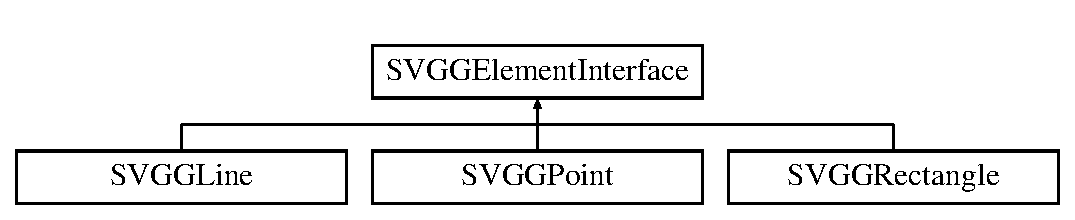
\includegraphics[height=2.000000cm]{classSVGGElementInterface}
\end{center}
\end{figure}
\subsection*{Public Member Functions}
\begin{DoxyCompactItemize}
\item 
\hypertarget{classSVGGElementInterface_ab1b44820b07e53aef0a06886c45031ec}{
virtual void {\bfseries Draw} (float XFactor, float YFactor, StreamInterface \&out)=0}
\label{classSVGGElementInterface_ab1b44820b07e53aef0a06886c45031ec}

\item 
\hypertarget{classSVGGElementInterface_ac6b542f4b5349350b4da6ff88c8e399a}{
void {\bfseries SetColor} (SVGGColor color, StreamInterface \&out)}
\label{classSVGGElementInterface_ac6b542f4b5349350b4da6ff88c8e399a}

\end{DoxyCompactItemize}


The documentation for this class was generated from the following file:\begin{DoxyCompactItemize}
\item 
SVGGraph.h\end{DoxyCompactItemize}

\hypertarget{classSVGGLine}{
\section{SVGGLine Class Reference}
\label{classSVGGLine}\index{SVGGLine@{SVGGLine}}
}
Inheritance diagram for SVGGLine:\begin{figure}[H]
\begin{center}
\leavevmode
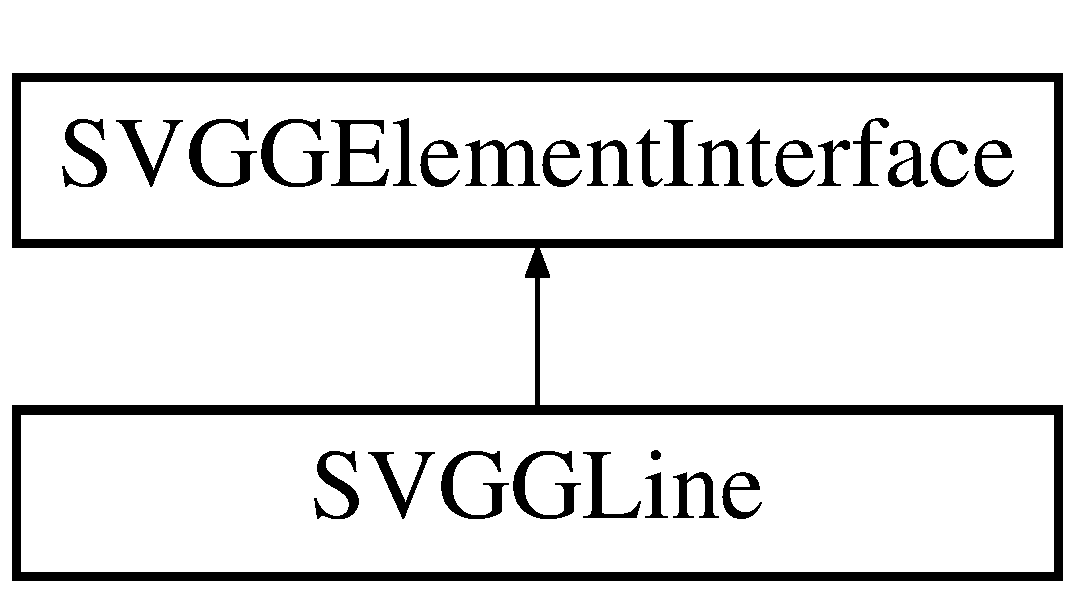
\includegraphics[height=2.000000cm]{classSVGGLine}
\end{center}
\end{figure}
\subsection*{Public Member Functions}
\begin{DoxyCompactItemize}
\item 
\hypertarget{classSVGGLine_a85498ae7a7c767546299b51df4b7a284}{
virtual void {\bfseries Draw} (float XFactor, float YFactor, StreamInterface \&out)}
\label{classSVGGLine_a85498ae7a7c767546299b51df4b7a284}

\end{DoxyCompactItemize}
\subsection*{Public Attributes}
\begin{DoxyCompactItemize}
\item 
\hypertarget{classSVGGLine_a74618f36cfd1a034932ed9460c823da2}{
float {\bfseries x1}}
\label{classSVGGLine_a74618f36cfd1a034932ed9460c823da2}

\item 
\hypertarget{classSVGGLine_a6b35e91038522cc76e3fc5659970ff1b}{
float {\bfseries y1}}
\label{classSVGGLine_a6b35e91038522cc76e3fc5659970ff1b}

\item 
\hypertarget{classSVGGLine_a0c16b37f656ff28a9c3e0e580d178b1a}{
float {\bfseries x2}}
\label{classSVGGLine_a0c16b37f656ff28a9c3e0e580d178b1a}

\item 
\hypertarget{classSVGGLine_aa36e24b6e689f4d8e8da2b82203de3c5}{
float {\bfseries y2}}
\label{classSVGGLine_aa36e24b6e689f4d8e8da2b82203de3c5}

\item 
\hypertarget{classSVGGLine_a35cdde66a9a3cd341b9b48675f4e746d}{
int {\bfseries lineWidth}}
\label{classSVGGLine_a35cdde66a9a3cd341b9b48675f4e746d}

\item 
\hypertarget{classSVGGLine_adf4a0c03ed8a73cf03493625974fb15f}{
SVGGLineType {\bfseries lineType}}
\label{classSVGGLine_adf4a0c03ed8a73cf03493625974fb15f}

\item 
\hypertarget{classSVGGLine_ac486898bab4a78743c3393c4dd7d94da}{
SVGGColor {\bfseries color}}
\label{classSVGGLine_ac486898bab4a78743c3393c4dd7d94da}

\end{DoxyCompactItemize}


The documentation for this class was generated from the following file:\begin{DoxyCompactItemize}
\item 
SVGGraph.h\end{DoxyCompactItemize}

\hypertarget{classSVGGPoint}{
\section{SVGGPoint Class Reference}
\label{classSVGGPoint}\index{SVGGPoint@{SVGGPoint}}
}
Inheritance diagram for SVGGPoint:\begin{figure}[H]
\begin{center}
\leavevmode
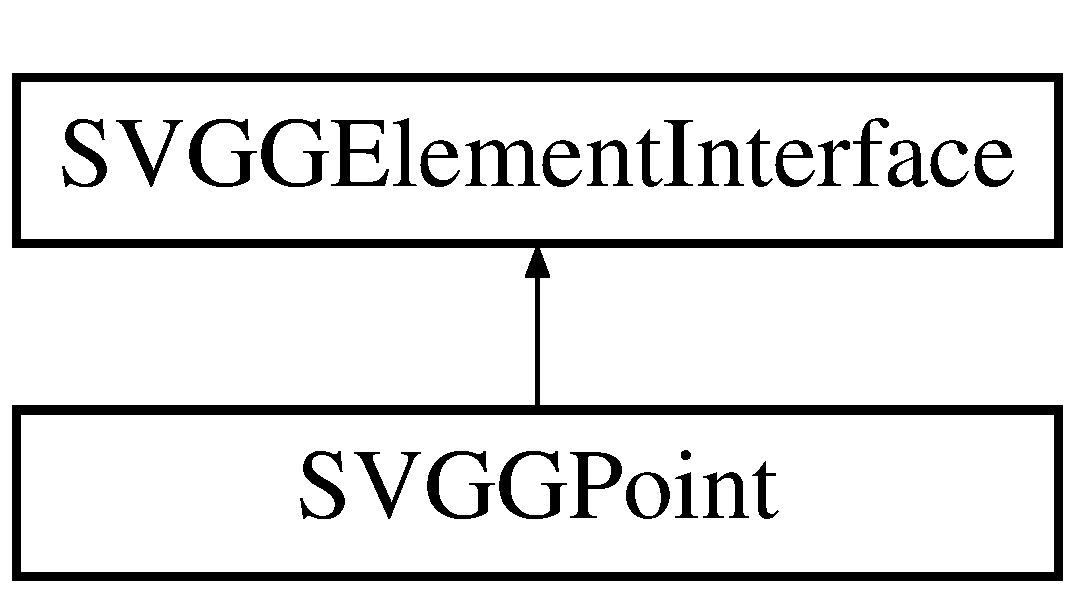
\includegraphics[height=2.000000cm]{classSVGGPoint}
\end{center}
\end{figure}
\subsection*{Public Member Functions}
\begin{DoxyCompactItemize}
\item 
\hypertarget{classSVGGPoint_acc2cd157fe0a89b0a02f048da38d94fd}{
virtual void {\bfseries Draw} (float XFactor, float YFactor, StreamInterface \&out)}
\label{classSVGGPoint_acc2cd157fe0a89b0a02f048da38d94fd}

\end{DoxyCompactItemize}
\subsection*{Public Attributes}
\begin{DoxyCompactItemize}
\item 
\hypertarget{classSVGGPoint_a06824ed5ca0622e9abba18bca6879f74}{
float {\bfseries x}}
\label{classSVGGPoint_a06824ed5ca0622e9abba18bca6879f74}

\item 
\hypertarget{classSVGGPoint_a01b94c6f8b1bb006797219773d71054d}{
float {\bfseries y}}
\label{classSVGGPoint_a01b94c6f8b1bb006797219773d71054d}

\item 
\hypertarget{classSVGGPoint_a310903f98b5981ee4ca073b5a6c4b0d2}{
SVGGPointType {\bfseries pointType}}
\label{classSVGGPoint_a310903f98b5981ee4ca073b5a6c4b0d2}

\item 
\hypertarget{classSVGGPoint_adf6e6c9b829965ae2ee54a1bb8a9bd19}{
int {\bfseries size}}
\label{classSVGGPoint_adf6e6c9b829965ae2ee54a1bb8a9bd19}

\item 
\hypertarget{classSVGGPoint_ad2255ea00c9f3ccc3260b1b87524e6e4}{
SVGGColor {\bfseries color}}
\label{classSVGGPoint_ad2255ea00c9f3ccc3260b1b87524e6e4}

\end{DoxyCompactItemize}


The documentation for this class was generated from the following file:\begin{DoxyCompactItemize}
\item 
SVGGraph.h\end{DoxyCompactItemize}

\hypertarget{classSVGGraph}{
\section{SVGGraph Class Reference}
\label{classSVGGraph}\index{SVGGraph@{SVGGraph}}
}
\subsection*{Public Member Functions}
\begin{DoxyCompactItemize}
\item 
\hypertarget{classSVGGraph_af9021475ffc34852a1a3e2a5ba18f4fc}{
void {\bfseries AddPoint} (float xCoord, float yCoord, SVGGPointType type, SVGGColor color, int lineWidth)}
\label{classSVGGraph_af9021475ffc34852a1a3e2a5ba18f4fc}

\item 
\hypertarget{classSVGGraph_a642fa30fa185765503ea997720255f23}{
void {\bfseries AddLine} (float x1, float y1, float x2, float y2, SVGGLineType lineType, SVGGColor color, int lineWidth)}
\label{classSVGGraph_a642fa30fa185765503ea997720255f23}

\item 
\hypertarget{classSVGGraph_a519f5d1c9dcc2ea906e7b778826419cf}{
void {\bfseries AddRectangle} (float x, float y, float width, float height, SVGGLineType lineType, SVGGColor areaColor, SVGGColor lineColor, int lineWidth)}
\label{classSVGGraph_a519f5d1c9dcc2ea906e7b778826419cf}

\item 
\hypertarget{classSVGGraph_a97af80ab95d6713fc8d44327edbc2218}{
void {\bfseries Draw} (StreamInterface \&out)}
\label{classSVGGraph_a97af80ab95d6713fc8d44327edbc2218}

\end{DoxyCompactItemize}
\subsection*{Public Attributes}
\begin{DoxyCompactItemize}
\item 
\hypertarget{classSVGGraph_aef84f037dd29dcc5e12226b301dacc7a}{
int {\bfseries xSize}}
\label{classSVGGraph_aef84f037dd29dcc5e12226b301dacc7a}

\item 
\hypertarget{classSVGGraph_ac290e5e0d59a084595fc8b60cc294f53}{
int {\bfseries ySize}}
\label{classSVGGraph_ac290e5e0d59a084595fc8b60cc294f53}

\item 
\hypertarget{classSVGGraph_a07c3706546682b7c7c7b2cb40780f6ab}{
bool {\bfseries grid}}
\label{classSVGGraph_a07c3706546682b7c7c7b2cb40780f6ab}

\item 
\hypertarget{classSVGGraph_a27248988a8b47ebe081b3f5117e37d6c}{
float {\bfseries gridDensity}}
\label{classSVGGraph_a27248988a8b47ebe081b3f5117e37d6c}

\item 
\hypertarget{classSVGGraph_ac7c7add94463436bdb5c4f30c1863b68}{
bool {\bfseries axes}}
\label{classSVGGraph_ac7c7add94463436bdb5c4f30c1863b68}

\end{DoxyCompactItemize}


The documentation for this class was generated from the following file:\begin{DoxyCompactItemize}
\item 
SVGGraph.h\end{DoxyCompactItemize}

\hypertarget{classSVGGRectangle}{
\section{SVGGRectangle Class Reference}
\label{classSVGGRectangle}\index{SVGGRectangle@{SVGGRectangle}}
}
Inheritance diagram for SVGGRectangle:\begin{figure}[H]
\begin{center}
\leavevmode
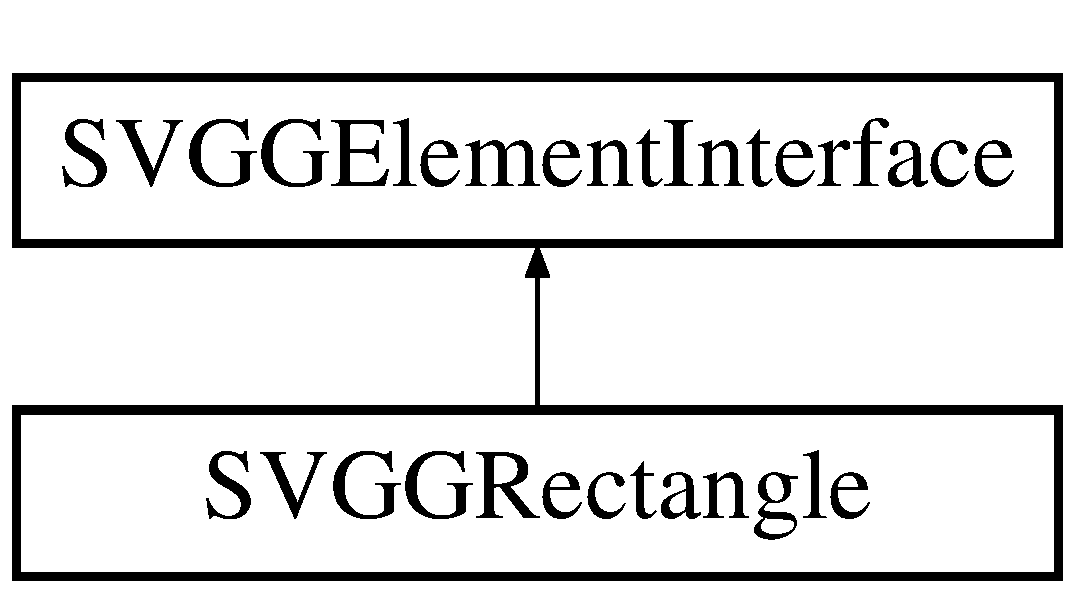
\includegraphics[height=2.000000cm]{classSVGGRectangle}
\end{center}
\end{figure}
\subsection*{Public Member Functions}
\begin{DoxyCompactItemize}
\item 
\hypertarget{classSVGGRectangle_a272fee1e0e03281b7f64b312cb3d4a85}{
virtual void {\bfseries Draw} (float XFactor, float YFactor, StreamInterface \&out)}
\label{classSVGGRectangle_a272fee1e0e03281b7f64b312cb3d4a85}

\end{DoxyCompactItemize}
\subsection*{Public Attributes}
\begin{DoxyCompactItemize}
\item 
\hypertarget{classSVGGRectangle_a9cbbd40377b1974ebb4d23e433c74c17}{
float {\bfseries x}}
\label{classSVGGRectangle_a9cbbd40377b1974ebb4d23e433c74c17}

\item 
\hypertarget{classSVGGRectangle_a09a4a21ab2e47aa66ac53f8176740a7e}{
float {\bfseries y}}
\label{classSVGGRectangle_a09a4a21ab2e47aa66ac53f8176740a7e}

\item 
\hypertarget{classSVGGRectangle_afd780bd3d34ad3a8be3091c4bb48b21a}{
float {\bfseries width}}
\label{classSVGGRectangle_afd780bd3d34ad3a8be3091c4bb48b21a}

\item 
\hypertarget{classSVGGRectangle_a97f5593a4715f352ebf803e106959433}{
float {\bfseries height}}
\label{classSVGGRectangle_a97f5593a4715f352ebf803e106959433}

\item 
\hypertarget{classSVGGRectangle_a327995b00c7597dc22eaf7d3218f8654}{
int {\bfseries lineWidth}}
\label{classSVGGRectangle_a327995b00c7597dc22eaf7d3218f8654}

\item 
\hypertarget{classSVGGRectangle_adb3b4586a44cab2e8c3607b7f3b09615}{
SVGGLineType {\bfseries lineType}}
\label{classSVGGRectangle_adb3b4586a44cab2e8c3607b7f3b09615}

\item 
\hypertarget{classSVGGRectangle_a72c7627565f2d54a4744256a67db10cc}{
SVGGColor {\bfseries lineColor}}
\label{classSVGGRectangle_a72c7627565f2d54a4744256a67db10cc}

\item 
\hypertarget{classSVGGRectangle_aadf7246100699d8f009bf0a32eb6a154}{
SVGGColor {\bfseries areaColor}}
\label{classSVGGRectangle_aadf7246100699d8f009bf0a32eb6a154}

\end{DoxyCompactItemize}


The documentation for this class was generated from the following file:\begin{DoxyCompactItemize}
\item 
SVGGraph.h\end{DoxyCompactItemize}

\hypertarget{structTypeList}{
\section{TypeList Struct Reference}
\label{structTypeList}\index{TypeList@{TypeList}}
}
\subsection*{Public Attributes}
\begin{DoxyCompactItemize}
\item 
\hypertarget{structTypeList_a3c0ae33a73e00ef08f72fa69b2c70114}{
char $\ast$ {\bfseries type}}
\label{structTypeList_a3c0ae33a73e00ef08f72fa69b2c70114}

\item 
\hypertarget{structTypeList_a0b31f04d29ccf89f134fc079f082c955}{
char $\ast$ {\bfseries modif}}
\label{structTypeList_a0b31f04d29ccf89f134fc079f082c955}

\item 
\hypertarget{structTypeList_a42e259d68c39b7315008cf044f5e6623}{
int {\bfseries size}}
\label{structTypeList_a42e259d68c39b7315008cf044f5e6623}

\item 
\hypertarget{structTypeList_aa0490d4be714cdda35fade2ba3f952d4}{
TypeListFn {\bfseries display}}
\label{structTypeList_aa0490d4be714cdda35fade2ba3f952d4}

\end{DoxyCompactItemize}


The documentation for this struct was generated from the following file:\begin{DoxyCompactItemize}
\item 
ObjectBrowserMenu.cpp\end{DoxyCompactItemize}

\hypertarget{classWaveform}{
\section{Waveform Class Reference}
\label{classWaveform}\index{Waveform@{Waveform}}
}


{\ttfamily \#include $<$Waveform.h$>$}

Inheritance diagram for Waveform:\begin{figure}[H]
\begin{center}
\leavevmode
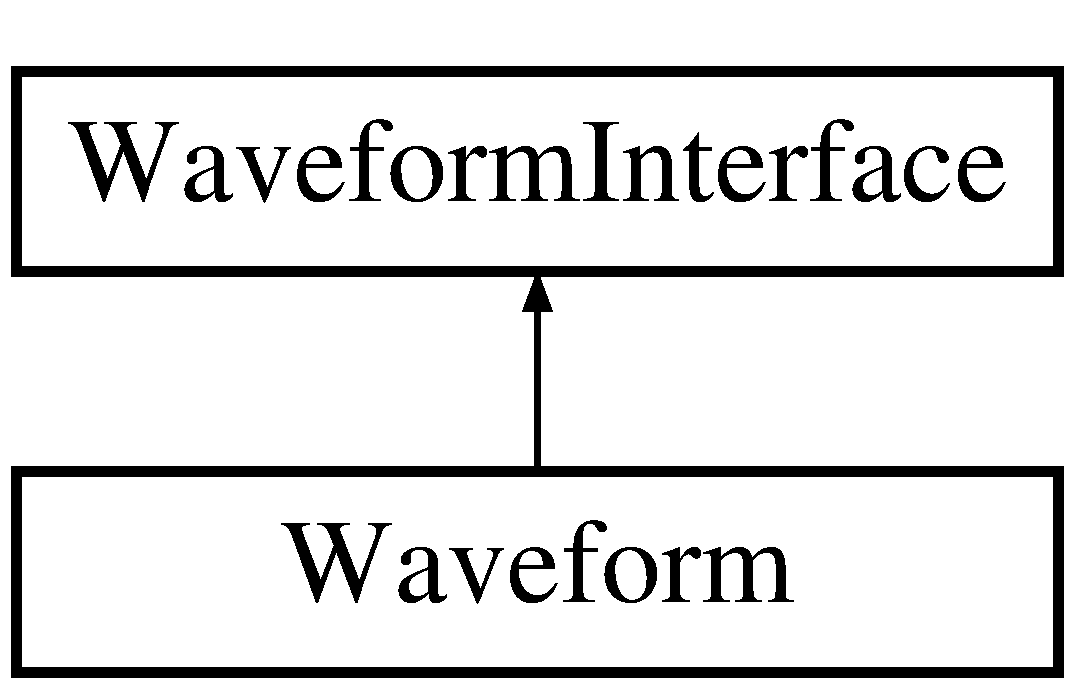
\includegraphics[height=2.000000cm]{classWaveform}
\end{center}
\end{figure}
\subsection*{Public Member Functions}
\begin{DoxyCompactItemize}
\item 
\hyperlink{classWaveform_a4a10db706dde8126a190a650f0b639fb}{Waveform} ()
\item 
virtual \hyperlink{classWaveform_afe871149df16f9cd13db35327c2b18b4}{$\sim$Waveform} ()
\item 
virtual bool \hyperlink{classWaveform_a692472f16f4d52b2a1378b8f4a9ec979}{ObjectLoadSetup} (ConfigurationDataBase \&cdbData, StreamInterface $\ast$err)
\item 
virtual float \hyperlink{classWaveform_ad7063bc356998bd730c79345a97f6656}{GetValue} (int32 usecTime)
\item 
virtual void \hyperlink{classWaveform_acd7677715381b3e9edc15f25f55f8edb}{Reset} ()
\item 
\hypertarget{classWaveform_a5f8c1672244a62bd673e752e7a741222}{
virtual bool {\bfseries ProcessHttpMessage} (HttpStream \&hStream)}
\label{classWaveform_a5f8c1672244a62bd673e752e7a741222}

\item 
\hypertarget{classWaveform_a53510c056e86f9d93f95edcb13b3e816}{
void {\bfseries HTMLInfo} (HttpStream \&hStream)}
\label{classWaveform_a53510c056e86f9d93f95edcb13b3e816}

\item 
\hypertarget{classWaveform_a740fbd30b18492210592b685cfbb31de}{
\hyperlink{structWaveformData}{WaveformData} $\ast$ {\bfseries GetWaveformDataPointer} ()}
\label{classWaveform_a740fbd30b18492210592b685cfbb31de}

\item 
\hypertarget{classWaveform_a3fd5e0286b2234cc73cdce919bc286dd}{
int32 {\bfseries NumberOfWindows} ()}
\label{classWaveform_a3fd5e0286b2234cc73cdce919bc286dd}

\end{DoxyCompactItemize}


\subsection{Detailed Description}
A waveform which keeps its internal time in microseconds but loads data from CDB in seconds. Note that all slopes are calculated at the moment of creation (function ObjectLoadSetup), and that the waveform has to be resetted (function Reset) between a pulse and the other. 

\subsection{Constructor \& Destructor Documentation}
\hypertarget{classWaveform_a4a10db706dde8126a190a650f0b639fb}{
\index{Waveform@{Waveform}!Waveform@{Waveform}}
\index{Waveform@{Waveform}!Waveform@{Waveform}}
\subsubsection[{Waveform}]{\setlength{\rightskip}{0pt plus 5cm}Waveform::Waveform (
\begin{DoxyParamCaption}
{}
\end{DoxyParamCaption}
)\hspace{0.3cm}{\ttfamily  \mbox{[}inline\mbox{]}}}}
\label{classWaveform_a4a10db706dde8126a190a650f0b639fb}
Constructor \hypertarget{classWaveform_afe871149df16f9cd13db35327c2b18b4}{
\index{Waveform@{Waveform}!$\sim$Waveform@{$\sim$Waveform}}
\index{$\sim$Waveform@{$\sim$Waveform}!Waveform@{Waveform}}
\subsubsection[{$\sim$Waveform}]{\setlength{\rightskip}{0pt plus 5cm}virtual Waveform::$\sim$Waveform (
\begin{DoxyParamCaption}
{}
\end{DoxyParamCaption}
)\hspace{0.3cm}{\ttfamily  \mbox{[}inline, virtual\mbox{]}}}}
\label{classWaveform_afe871149df16f9cd13db35327c2b18b4}
Deconstructor 

\subsection{Member Function Documentation}
\hypertarget{classWaveform_ad7063bc356998bd730c79345a97f6656}{
\index{Waveform@{Waveform}!GetValue@{GetValue}}
\index{GetValue@{GetValue}!Waveform@{Waveform}}
\subsubsection[{GetValue}]{\setlength{\rightskip}{0pt plus 5cm}float Waveform::GetValue (
\begin{DoxyParamCaption}
\item[{int32}]{usecTime}
\end{DoxyParamCaption}
)\hspace{0.3cm}{\ttfamily  \mbox{[}virtual\mbox{]}}}}
\label{classWaveform_ad7063bc356998bd730c79345a97f6656}
Returns the value of the waveform at a certain time. 
\begin{DoxyParams}{Parameters}
{\em usecTime} & Time in microseconds. Note that usecTime needs to be crescent: in order to obtain the value of the waveform in the past you must Reset it first. \\
\hline
\end{DoxyParams}
\begin{DoxyReturn}{Returns}
The value of the waveform at the specified time. If usecTime is before or after the start or end time of the waveform, the first or last value is held. 
\end{DoxyReturn}


Implements \hyperlink{classWaveformInterface}{WaveformInterface}.

\hypertarget{classWaveform_a692472f16f4d52b2a1378b8f4a9ec979}{
\index{Waveform@{Waveform}!ObjectLoadSetup@{ObjectLoadSetup}}
\index{ObjectLoadSetup@{ObjectLoadSetup}!Waveform@{Waveform}}
\subsubsection[{ObjectLoadSetup}]{\setlength{\rightskip}{0pt plus 5cm}bool Waveform::ObjectLoadSetup (
\begin{DoxyParamCaption}
\item[{ConfigurationDataBase \&}]{cdbData, }
\item[{StreamInterface $\ast$}]{err}
\end{DoxyParamCaption}
)\hspace{0.3cm}{\ttfamily  \mbox{[}virtual\mbox{]}}}}
\label{classWaveform_a692472f16f4d52b2a1378b8f4a9ec979}
Loads parameters from a CDB 
\begin{DoxyParams}{Parameters}
{\em cdbData} & the CDB \\
\hline
\end{DoxyParams}
\begin{DoxyReturn}{Returns}
True if the initialisation went ok, False otherwise 
\end{DoxyReturn}
\hypertarget{classWaveform_acd7677715381b3e9edc15f25f55f8edb}{
\index{Waveform@{Waveform}!Reset@{Reset}}
\index{Reset@{Reset}!Waveform@{Waveform}}
\subsubsection[{Reset}]{\setlength{\rightskip}{0pt plus 5cm}virtual void Waveform::Reset (
\begin{DoxyParamCaption}
{}
\end{DoxyParamCaption}
)\hspace{0.3cm}{\ttfamily  \mbox{[}inline, virtual\mbox{]}}}}
\label{classWaveform_acd7677715381b3e9edc15f25f55f8edb}
Reset function. Resets the internal states and waveforms. To be called in the PREPULSE phase. 

Implements \hyperlink{classWaveformInterface}{WaveformInterface}.



The documentation for this class was generated from the following files:\begin{DoxyCompactItemize}
\item 
\hyperlink{Waveform_8h}{Waveform.h}\item 
Waveform.cpp\end{DoxyCompactItemize}

\hypertarget{structWaveformData}{
\section{WaveformData Struct Reference}
\label{structWaveformData}\index{WaveformData@{WaveformData}}
}


{\ttfamily \#include $<$Waveform.h$>$}

\subsection*{Public Attributes}
\begin{DoxyCompactItemize}
\item 
\hypertarget{structWaveformData_ac89ea88a20508737461c9a455f5329fc}{
int32 {\bfseries usecTime}}
\label{structWaveformData_ac89ea88a20508737461c9a455f5329fc}

\item 
\hypertarget{structWaveformData_a4008c00e5513f941725b97518d98e0e3}{
float {\bfseries amplitude}}
\label{structWaveformData_a4008c00e5513f941725b97518d98e0e3}

\item 
\hypertarget{structWaveformData_a2057bcb61284354ad64e63d97852db2c}{
float {\bfseries slope}}
\label{structWaveformData_a2057bcb61284354ad64e63d97852db2c}

\end{DoxyCompactItemize}


\subsection{Detailed Description}
Structure holding data for a single element in an \hyperlink{classIntegerWaveform}{IntegerWaveform}. 

The documentation for this struct was generated from the following file:\begin{DoxyCompactItemize}
\item 
\hyperlink{Waveform_8h}{Waveform.h}\end{DoxyCompactItemize}

\hypertarget{classWaveformInterface}{
\section{WaveformInterface Class Reference}
\label{classWaveformInterface}\index{WaveformInterface@{WaveformInterface}}
}
Inheritance diagram for WaveformInterface:\begin{figure}[H]
\begin{center}
\leavevmode
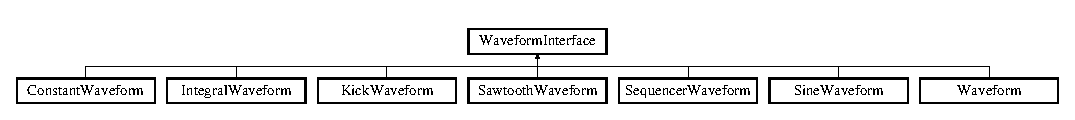
\includegraphics[height=1.159420cm]{classWaveformInterface}
\end{center}
\end{figure}
\subsection*{Public Member Functions}
\begin{DoxyCompactItemize}
\item 
\hypertarget{classWaveformInterface_aef679b3365b542ed5268b46d01f7f5a7}{
virtual float {\bfseries GetValue} (int32 usecTime)=0}
\label{classWaveformInterface_aef679b3365b542ed5268b46d01f7f5a7}

\item 
\hypertarget{classWaveformInterface_a466705327288a237be0f8623d9890291}{
virtual int32 {\bfseries GetValueInt32} (int32 usecTime)}
\label{classWaveformInterface_a466705327288a237be0f8623d9890291}

\item 
\hypertarget{classWaveformInterface_a25947afe4c1ada2e10a21dfaa7d8e8b5}{
virtual double {\bfseries GetValueD} (int32 usecTime)}
\label{classWaveformInterface_a25947afe4c1ada2e10a21dfaa7d8e8b5}

\item 
\hypertarget{classWaveformInterface_a7c78e14343080ee82cb6bdfe42d3f2b5}{
virtual float {\bfseries GetValue64} (int64 usecTime)}
\label{classWaveformInterface_a7c78e14343080ee82cb6bdfe42d3f2b5}

\item 
\hypertarget{classWaveformInterface_a54abdef10a194f21fbbfd9202d0a58df}{
virtual double {\bfseries GetValueD64} (int64 usecTime)}
\label{classWaveformInterface_a54abdef10a194f21fbbfd9202d0a58df}

\item 
\hypertarget{classWaveformInterface_a215fc20e03cdb25f95ebd461d7e30e87}{
virtual void {\bfseries Reset} ()=0}
\label{classWaveformInterface_a215fc20e03cdb25f95ebd461d7e30e87}

\end{DoxyCompactItemize}


The documentation for this class was generated from the following file:\begin{DoxyCompactItemize}
\item 
WaveformInterface.h\end{DoxyCompactItemize}

\hypertarget{classWindowsServiceApplication}{
\section{WindowsServiceApplication Class Reference}
\label{classWindowsServiceApplication}\index{WindowsServiceApplication@{WindowsServiceApplication}}
}


{\ttfamily \#include $<$WindowsServiceApplication.h$>$}

\subsection*{Public Member Functions}
\begin{DoxyCompactItemize}
\item 
bool \hyperlink{classWindowsServiceApplication_a04def6eaee00fa79d249d341dab7b11f}{Main} (int argc, char $\ast$$\ast$argv)
\item 
\hyperlink{classWindowsServiceApplication_ac4bc29d1d8efeba0190f6b4d5c99ae67}{WindowsServiceApplication} (const char $\ast$serviceName, const char $\ast$title)
\end{DoxyCompactItemize}
\subsection*{Friends}
\begin{DoxyCompactItemize}
\item 
bool \hyperlink{classWindowsServiceApplication_ab6e5bf4c1ae7515070871d380387d42b}{WSAMain} (\hyperlink{classWindowsServiceApplication}{WindowsServiceApplication} $\ast$wsa, int argc, char $\ast$$\ast$argv)
\end{DoxyCompactItemize}


\subsection{Detailed Description}
this class allow simple building of window services this only works on windows!! Only one instance of this class derivative can be used since the mechanism uses a global variable 

\subsection{Constructor \& Destructor Documentation}
\hypertarget{classWindowsServiceApplication_ac4bc29d1d8efeba0190f6b4d5c99ae67}{
\index{WindowsServiceApplication@{WindowsServiceApplication}!WindowsServiceApplication@{WindowsServiceApplication}}
\index{WindowsServiceApplication@{WindowsServiceApplication}!WindowsServiceApplication@{WindowsServiceApplication}}
\subsubsection[{WindowsServiceApplication}]{\setlength{\rightskip}{0pt plus 5cm}WindowsServiceApplication::WindowsServiceApplication (
\begin{DoxyParamCaption}
\item[{const char $\ast$}]{serviceName, }
\item[{const char $\ast$}]{title}
\end{DoxyParamCaption}
)\hspace{0.3cm}{\ttfamily  \mbox{[}inline\mbox{]}}}}
\label{classWindowsServiceApplication_ac4bc29d1d8efeba0190f6b4d5c99ae67}


\subsection{Member Function Documentation}
\hypertarget{classWindowsServiceApplication_a04def6eaee00fa79d249d341dab7b11f}{
\index{WindowsServiceApplication@{WindowsServiceApplication}!Main@{Main}}
\index{Main@{Main}!WindowsServiceApplication@{WindowsServiceApplication}}
\subsubsection[{Main}]{\setlength{\rightskip}{0pt plus 5cm}bool WindowsServiceApplication::Main (
\begin{DoxyParamCaption}
\item[{int}]{argc, }
\item[{char $\ast$$\ast$}]{argv}
\end{DoxyParamCaption}
)\hspace{0.3cm}{\ttfamily  \mbox{[}inline\mbox{]}}}}
\label{classWindowsServiceApplication_a04def6eaee00fa79d249d341dab7b11f}


\subsection{Friends And Related Function Documentation}
\hypertarget{classWindowsServiceApplication_ab6e5bf4c1ae7515070871d380387d42b}{
\index{WindowsServiceApplication@{WindowsServiceApplication}!WSAMain@{WSAMain}}
\index{WSAMain@{WSAMain}!WindowsServiceApplication@{WindowsServiceApplication}}
\subsubsection[{WSAMain}]{\setlength{\rightskip}{0pt plus 5cm}bool WSAMain (
\begin{DoxyParamCaption}
\item[{{\bf WindowsServiceApplication} $\ast$}]{wsa, }
\item[{int}]{argc, }
\item[{char $\ast$$\ast$}]{argv}
\end{DoxyParamCaption}
)\hspace{0.3cm}{\ttfamily  \mbox{[}friend\mbox{]}}}}
\label{classWindowsServiceApplication_ab6e5bf4c1ae7515070871d380387d42b}


The documentation for this class was generated from the following file:\begin{DoxyCompactItemize}
\item 
\hyperlink{WindowsServiceApplication_8h}{WindowsServiceApplication.h}\end{DoxyCompactItemize}

\chapter{File Documentation}
\hypertarget{BaseLib2CInterface_8h}{
\section{BaseLib2CInterface.h File Reference}
\label{BaseLib2CInterface_8h}\index{BaseLib2CInterface.h@{BaseLib2CInterface.h}}
}


C interface for BaseLib2.  


{\ttfamily \#include \char`\"{}CDBCInterface.h\char`\"{}}\par
\subsection*{Functions}
\begin{DoxyCompactItemize}
\item 
int \hyperlink{BaseLib2CInterface_8h_a0cc16156309f703ea43ed3ebbe33308d}{B2C\_\-CreateGODBObject} (const char $\ast$context, const char $\ast$className, const char $\ast$objectName)
\item 
int \hyperlink{BaseLib2CInterface_8h_a7c9e8dd4a4322555ea266d1ececb0c3f}{B2C\_\-CreateAndInitialiseGODBObject} (const char $\ast$context, CDBReference configuration)
\item 
int \hyperlink{BaseLib2CInterface_8h_af0ecdbebb94b802693c600e1fab821cc}{B2C\_\-InitialiseGODBObject} (const char $\ast$context, CDBReference configuration)
\item 
int \hyperlink{BaseLib2CInterface_8h_aec65245b4bd7dc8349cef17f4c1840ce}{B2C\_\-DeleteGODBSubTree} (const char $\ast$context, int deleteThisNode)
\item 
int \hyperlink{BaseLib2CInterface_8h_ae028161cbda18aea9d702feebd27f338}{B2C\_\-ListGODBNodes} (const char $\ast$context, int order, char $\ast$objectName, char $\ast$className, int bufferSize, int $\ast$containerClass)
\item 
int \hyperlink{BaseLib2CInterface_8h_aca10c6a286e737ae5853b1a1b6cb4e87}{B2C\_\-ShowGODBSubTree} (const char $\ast$context, char $\ast$output, int bufferSize)
\item 
int \hyperlink{BaseLib2CInterface_8h_aba5597b73986877f888b06a30167e79f}{B2C\_\-SendMessageToGODBObject} (const char $\ast$context, const char $\ast$messageText, int messageCode)
\end{DoxyCompactItemize}


\subsection{Detailed Description}
C interface for BaseLib2. 

\subsection{Function Documentation}
\hypertarget{BaseLib2CInterface_8h_a7c9e8dd4a4322555ea266d1ececb0c3f}{
\index{BaseLib2CInterface.h@{BaseLib2CInterface.h}!B2C\_\-CreateAndInitialiseGODBObject@{B2C\_\-CreateAndInitialiseGODBObject}}
\index{B2C\_\-CreateAndInitialiseGODBObject@{B2C\_\-CreateAndInitialiseGODBObject}!BaseLib2CInterface.h@{BaseLib2CInterface.h}}
\subsubsection[{B2C\_\-CreateAndInitialiseGODBObject}]{\setlength{\rightskip}{0pt plus 5cm}int B2C\_\-CreateAndInitialiseGODBObject (
\begin{DoxyParamCaption}
\item[{const char $\ast$}]{context, }
\item[{CDBReference}]{configuration}
\end{DoxyParamCaption}
)}}
\label{BaseLib2CInterface_8h_a7c9e8dd4a4322555ea266d1ececb0c3f}
create an object to be inserted in the present GODB location (must be a container node) the object class, name and initialisation data is taken from CDB current subtree the object name is the current node name the object class is obtained from the ClassName leaf all the other leafs and sub-\/subtrees are for the object to use to initialise itself returns 0 on success return -\/1 if context is a wrong path \hypertarget{BaseLib2CInterface_8h_a0cc16156309f703ea43ed3ebbe33308d}{
\index{BaseLib2CInterface.h@{BaseLib2CInterface.h}!B2C\_\-CreateGODBObject@{B2C\_\-CreateGODBObject}}
\index{B2C\_\-CreateGODBObject@{B2C\_\-CreateGODBObject}!BaseLib2CInterface.h@{BaseLib2CInterface.h}}
\subsubsection[{B2C\_\-CreateGODBObject}]{\setlength{\rightskip}{0pt plus 5cm}int B2C\_\-CreateGODBObject (
\begin{DoxyParamCaption}
\item[{const char $\ast$}]{context, }
\item[{const char $\ast$}]{className, }
\item[{const char $\ast$}]{objectName}
\end{DoxyParamCaption}
)}}
\label{BaseLib2CInterface_8h_a0cc16156309f703ea43ed3ebbe33308d}
create an object of className and objectName it works if class exists and is of the right type (GCNamedObject derivative) the object is located in the path specified by context returns 0 on success return -\/1 if context is a wrong path \hypertarget{BaseLib2CInterface_8h_aec65245b4bd7dc8349cef17f4c1840ce}{
\index{BaseLib2CInterface.h@{BaseLib2CInterface.h}!B2C\_\-DeleteGODBSubTree@{B2C\_\-DeleteGODBSubTree}}
\index{B2C\_\-DeleteGODBSubTree@{B2C\_\-DeleteGODBSubTree}!BaseLib2CInterface.h@{BaseLib2CInterface.h}}
\subsubsection[{B2C\_\-DeleteGODBSubTree}]{\setlength{\rightskip}{0pt plus 5cm}int B2C\_\-DeleteGODBSubTree (
\begin{DoxyParamCaption}
\item[{const char $\ast$}]{context, }
\item[{int}]{deleteThisNode}
\end{DoxyParamCaption}
)}}
\label{BaseLib2CInterface_8h_aec65245b4bd7dc8349cef17f4c1840ce}
delete the current subtree of the GODB deleteThisNode = 1 remove the container from ddb returns 0 on success return -\/1 if context is a wrong path

delete the current subtree of the GODB returns 0 on success return -\/1 if context is a wrong path \hypertarget{BaseLib2CInterface_8h_af0ecdbebb94b802693c600e1fab821cc}{
\index{BaseLib2CInterface.h@{BaseLib2CInterface.h}!B2C\_\-InitialiseGODBObject@{B2C\_\-InitialiseGODBObject}}
\index{B2C\_\-InitialiseGODBObject@{B2C\_\-InitialiseGODBObject}!BaseLib2CInterface.h@{BaseLib2CInterface.h}}
\subsubsection[{B2C\_\-InitialiseGODBObject}]{\setlength{\rightskip}{0pt plus 5cm}int B2C\_\-InitialiseGODBObject (
\begin{DoxyParamCaption}
\item[{const char $\ast$}]{context, }
\item[{CDBReference}]{configuration}
\end{DoxyParamCaption}
)}}
\label{BaseLib2CInterface_8h_af0ecdbebb94b802693c600e1fab821cc}
configuration is a CDB reference pointing to the subtree containing the desired configuration data This call configures the object does not create a new object to be inserted returns 0 on success return -\/1 if context is a wrong path \hypertarget{BaseLib2CInterface_8h_ae028161cbda18aea9d702feebd27f338}{
\index{BaseLib2CInterface.h@{BaseLib2CInterface.h}!B2C\_\-ListGODBNodes@{B2C\_\-ListGODBNodes}}
\index{B2C\_\-ListGODBNodes@{B2C\_\-ListGODBNodes}!BaseLib2CInterface.h@{BaseLib2CInterface.h}}
\subsubsection[{B2C\_\-ListGODBNodes}]{\setlength{\rightskip}{0pt plus 5cm}int B2C\_\-ListGODBNodes (
\begin{DoxyParamCaption}
\item[{const char $\ast$}]{context, }
\item[{int}]{order, }
\item[{char $\ast$}]{objectName, }
\item[{char $\ast$}]{className, }
\item[{int}]{bufferSize, }
\item[{int $\ast$}]{containerClass}
\end{DoxyParamCaption}
)}}
\label{BaseLib2CInterface_8h_ae028161cbda18aea9d702feebd27f338}
describes the current subtree or its children order = -\/1 ==$>$ current node order $>$= 0 ==$>$ child i-\/th ObjectName ClassName must be pointers to buffers of size bufferSize containerClass is the pointer to an integer which returns 0 on success return -\/1 if context is a wrong path \hypertarget{BaseLib2CInterface_8h_aba5597b73986877f888b06a30167e79f}{
\index{BaseLib2CInterface.h@{BaseLib2CInterface.h}!B2C\_\-SendMessageToGODBObject@{B2C\_\-SendMessageToGODBObject}}
\index{B2C\_\-SendMessageToGODBObject@{B2C\_\-SendMessageToGODBObject}!BaseLib2CInterface.h@{BaseLib2CInterface.h}}
\subsubsection[{B2C\_\-SendMessageToGODBObject}]{\setlength{\rightskip}{0pt plus 5cm}int B2C\_\-SendMessageToGODBObject (
\begin{DoxyParamCaption}
\item[{const char $\ast$}]{context, }
\item[{const char $\ast$}]{messageText, }
\item[{int}]{messageCode}
\end{DoxyParamCaption}
)}}
\label{BaseLib2CInterface_8h_aba5597b73986877f888b06a30167e79f}
sends a message to an object within GODB returns 0 on success return -\/1 if context is a wrong path \hypertarget{BaseLib2CInterface_8h_aca10c6a286e737ae5853b1a1b6cb4e87}{
\index{BaseLib2CInterface.h@{BaseLib2CInterface.h}!B2C\_\-ShowGODBSubTree@{B2C\_\-ShowGODBSubTree}}
\index{B2C\_\-ShowGODBSubTree@{B2C\_\-ShowGODBSubTree}!BaseLib2CInterface.h@{BaseLib2CInterface.h}}
\subsubsection[{B2C\_\-ShowGODBSubTree}]{\setlength{\rightskip}{0pt plus 5cm}int B2C\_\-ShowGODBSubTree (
\begin{DoxyParamCaption}
\item[{const char $\ast$}]{context, }
\item[{char $\ast$}]{output, }
\item[{int}]{bufferSize}
\end{DoxyParamCaption}
)}}
\label{BaseLib2CInterface_8h_aca10c6a286e737ae5853b1a1b6cb4e87}
dumps the current subtree returns 0 on success return -\/1 if context is a wrong path 
\hypertarget{CDBBrowserMenu_8h}{
\section{CDBBrowserMenu.h File Reference}
\label{CDBBrowserMenu_8h}\index{CDBBrowserMenu.h@{CDBBrowserMenu.h}}
}


Enables the browsing of a ConfigurationDataBase.  


{\ttfamily \#include \char`\"{}MenuEntry.h\char`\"{}}\par
{\ttfamily \#include \char`\"{}CDBHtmlUtilities.h\char`\"{}}\par
\subsection*{Classes}
\begin{DoxyCompactItemize}
\item 
class \hyperlink{classCDBBrowserMenu}{CDBBrowserMenu}
\end{DoxyCompactItemize}
\subsection*{Functions}
\begin{DoxyCompactItemize}
\item 
bool \hyperlink{CDBBrowserMenu_8h_a785f26d21061253c713569b566b66644}{CDB2Browse} (StreamInterface \&in, StreamInterface \&out, ConfigurationDataBase \&cdbRef, const char $\ast$cdbName)
\item 
bool \hyperlink{CDBBrowserMenu_8h_a0f2e4df78baa29b840ff920877e3a35b}{CDB2Setup} (\hyperlink{classCDBBrowserMenu}{CDBBrowserMenu} \&cdbBrowse, const char $\ast$cdbName, ConfigurationDataBase \&cdbRef)
\end{DoxyCompactItemize}


\subsection{Detailed Description}
Enables the browsing of a ConfigurationDataBase. 

\subsection{Function Documentation}
\hypertarget{CDBBrowserMenu_8h_a785f26d21061253c713569b566b66644}{
\index{CDBBrowserMenu.h@{CDBBrowserMenu.h}!CDB2Browse@{CDB2Browse}}
\index{CDB2Browse@{CDB2Browse}!CDBBrowserMenu.h@{CDBBrowserMenu.h}}
\subsubsection[{CDB2Browse}]{\setlength{\rightskip}{0pt plus 5cm}bool CDB2Browse (
\begin{DoxyParamCaption}
\item[{StreamInterface \&}]{in, }
\item[{StreamInterface \&}]{out, }
\item[{ConfigurationDataBase \&}]{cdbRef, }
\item[{const char $\ast$}]{cdbName}
\end{DoxyParamCaption}
)}}
\label{CDBBrowserMenu_8h_a785f26d21061253c713569b566b66644}
\hypertarget{CDBBrowserMenu_8h_a0f2e4df78baa29b840ff920877e3a35b}{
\index{CDBBrowserMenu.h@{CDBBrowserMenu.h}!CDB2Setup@{CDB2Setup}}
\index{CDB2Setup@{CDB2Setup}!CDBBrowserMenu.h@{CDBBrowserMenu.h}}
\subsubsection[{CDB2Setup}]{\setlength{\rightskip}{0pt plus 5cm}bool CDB2Setup (
\begin{DoxyParamCaption}
\item[{{\bf CDBBrowserMenu} \&}]{cdbBrowse, }
\item[{const char $\ast$}]{cdbName, }
\item[{ConfigurationDataBase \&}]{cdbRef}
\end{DoxyParamCaption}
)}}
\label{CDBBrowserMenu_8h_a0f2e4df78baa29b840ff920877e3a35b}

\hypertarget{CDBHtmlUtilities_8h}{
\section{CDBHtmlUtilities.h File Reference}
\label{CDBHtmlUtilities_8h}\index{CDBHtmlUtilities.h@{CDBHtmlUtilities.h}}
}


Utility implementations to provide the interface between a CDB and HTML.  


{\ttfamily \#include \char`\"{}ConfigurationDataBase.h\char`\"{}}\par
{\ttfamily \#include \char`\"{}HttpStream.h\char`\"{}}\par
\subsection*{Typedefs}
\begin{DoxyCompactItemize}
\item 
typedef int \hyperlink{CDBHtmlUtilities_8h_a3c31a4130c52d0728f5c691565de650b}{CDBHUMode}
\end{DoxyCompactItemize}
\subsection*{Functions}
\begin{DoxyCompactItemize}
\item 
bool \hyperlink{CDBHtmlUtilities_8h_ac7581a96cbcabcc302ed6649be4b66da}{CDBHUHtmlObjectSubView} (ConfigurationDataBase \&cdb\_\-, const char $\ast$title\_\-, HttpStream \&hStream, \hyperlink{CDBHtmlUtilities_8h_a3c31a4130c52d0728f5c691565de650b}{CDBHUMode} mode)
\end{DoxyCompactItemize}
\subsection*{Variables}
\begin{DoxyCompactItemize}
\item 
const \hyperlink{CDBHtmlUtilities_8h_a3c31a4130c52d0728f5c691565de650b}{CDBHUMode} \hyperlink{CDBHtmlUtilities_8h_afcb8e89ba86e30c1e19cd5b933c23a7c}{CDBHUHOSUV\_\-Header} = 0x1
\item 
const \hyperlink{CDBHtmlUtilities_8h_a3c31a4130c52d0728f5c691565de650b}{CDBHUMode} \hyperlink{CDBHtmlUtilities_8h_a4e266d67a4f8ef6f5ce94453c1463d51}{CDBHUHOSUV\_\-Script} = 0x2
\item 
const \hyperlink{CDBHtmlUtilities_8h_a3c31a4130c52d0728f5c691565de650b}{CDBHUMode} \hyperlink{CDBHtmlUtilities_8h_a96593681b579cd1c2c19580e2c3d1e9d}{CDBHUHOSUV\_\-Body} = 0x4
\item 
const \hyperlink{CDBHtmlUtilities_8h_a3c31a4130c52d0728f5c691565de650b}{CDBHUMode} \hyperlink{CDBHtmlUtilities_8h_adb2dc40b6ce57efa7e80f8e35578a15f}{CDBHUHOSUV\_\-FullBody} = 0x8
\item 
const \hyperlink{CDBHtmlUtilities_8h_a3c31a4130c52d0728f5c691565de650b}{CDBHUMode} \hyperlink{CDBHtmlUtilities_8h_a609a3980c4f7ad725c9611205e49a3a9}{CDBHUHOSUV\_\-NoBack} = 0x10
\end{DoxyCompactItemize}


\subsection{Detailed Description}
Utility implementations to provide the interface between a CDB and HTML. 

\subsection{Typedef Documentation}
\hypertarget{CDBHtmlUtilities_8h_a3c31a4130c52d0728f5c691565de650b}{
\index{CDBHtmlUtilities.h@{CDBHtmlUtilities.h}!CDBHUMode@{CDBHUMode}}
\index{CDBHUMode@{CDBHUMode}!CDBHtmlUtilities.h@{CDBHtmlUtilities.h}}
\subsubsection[{CDBHUMode}]{\setlength{\rightskip}{0pt plus 5cm}typedef int {\bf CDBHUMode}}}
\label{CDBHtmlUtilities_8h_a3c31a4130c52d0728f5c691565de650b}
to specify what part of the webpage to produce 

\subsection{Function Documentation}
\hypertarget{CDBHtmlUtilities_8h_ac7581a96cbcabcc302ed6649be4b66da}{
\index{CDBHtmlUtilities.h@{CDBHtmlUtilities.h}!CDBHUHtmlObjectSubView@{CDBHUHtmlObjectSubView}}
\index{CDBHUHtmlObjectSubView@{CDBHUHtmlObjectSubView}!CDBHtmlUtilities.h@{CDBHtmlUtilities.h}}
\subsubsection[{CDBHUHtmlObjectSubView}]{\setlength{\rightskip}{0pt plus 5cm}bool CDBHUHtmlObjectSubView (
\begin{DoxyParamCaption}
\item[{ConfigurationDataBase \&}]{cdb\_\-, }
\item[{const char $\ast$}]{title\_\-, }
\item[{HttpStream \&}]{hStream, }
\item[{{\bf CDBHUMode}}]{mode}
\end{DoxyParamCaption}
)}}
\label{CDBHtmlUtilities_8h_ac7581a96cbcabcc302ed6649be4b66da}
allows implementing a browsing functionality for CDBVirtual derived databases 

\subsection{Variable Documentation}
\hypertarget{CDBHtmlUtilities_8h_a96593681b579cd1c2c19580e2c3d1e9d}{
\index{CDBHtmlUtilities.h@{CDBHtmlUtilities.h}!CDBHUHOSUV\_\-Body@{CDBHUHOSUV\_\-Body}}
\index{CDBHUHOSUV\_\-Body@{CDBHUHOSUV\_\-Body}!CDBHtmlUtilities.h@{CDBHtmlUtilities.h}}
\subsubsection[{CDBHUHOSUV\_\-Body}]{\setlength{\rightskip}{0pt plus 5cm}const {\bf CDBHUMode} {\bf CDBHUHOSUV\_\-Body} = 0x4}}
\label{CDBHtmlUtilities_8h_a96593681b579cd1c2c19580e2c3d1e9d}
the body part without BODY statement \hypertarget{CDBHtmlUtilities_8h_adb2dc40b6ce57efa7e80f8e35578a15f}{
\index{CDBHtmlUtilities.h@{CDBHtmlUtilities.h}!CDBHUHOSUV\_\-FullBody@{CDBHUHOSUV\_\-FullBody}}
\index{CDBHUHOSUV\_\-FullBody@{CDBHUHOSUV\_\-FullBody}!CDBHtmlUtilities.h@{CDBHtmlUtilities.h}}
\subsubsection[{CDBHUHOSUV\_\-FullBody}]{\setlength{\rightskip}{0pt plus 5cm}const {\bf CDBHUMode} {\bf CDBHUHOSUV\_\-FullBody} = 0x8}}
\label{CDBHtmlUtilities_8h_adb2dc40b6ce57efa7e80f8e35578a15f}
the body part with BODY statement \hypertarget{CDBHtmlUtilities_8h_afcb8e89ba86e30c1e19cd5b933c23a7c}{
\index{CDBHtmlUtilities.h@{CDBHtmlUtilities.h}!CDBHUHOSUV\_\-Header@{CDBHUHOSUV\_\-Header}}
\index{CDBHUHOSUV\_\-Header@{CDBHUHOSUV\_\-Header}!CDBHtmlUtilities.h@{CDBHtmlUtilities.h}}
\subsubsection[{CDBHUHOSUV\_\-Header}]{\setlength{\rightskip}{0pt plus 5cm}const {\bf CDBHUMode} {\bf CDBHUHOSUV\_\-Header} = 0x1}}
\label{CDBHtmlUtilities_8h_afcb8e89ba86e30c1e19cd5b933c23a7c}
all the header \hypertarget{CDBHtmlUtilities_8h_a609a3980c4f7ad725c9611205e49a3a9}{
\index{CDBHtmlUtilities.h@{CDBHtmlUtilities.h}!CDBHUHOSUV\_\-NoBack@{CDBHUHOSUV\_\-NoBack}}
\index{CDBHUHOSUV\_\-NoBack@{CDBHUHOSUV\_\-NoBack}!CDBHtmlUtilities.h@{CDBHtmlUtilities.h}}
\subsubsection[{CDBHUHOSUV\_\-NoBack}]{\setlength{\rightskip}{0pt plus 5cm}const {\bf CDBHUMode} {\bf CDBHUHOSUV\_\-NoBack} = 0x10}}
\label{CDBHtmlUtilities_8h_a609a3980c4f7ad725c9611205e49a3a9}
the body part has no Back statement \hypertarget{CDBHtmlUtilities_8h_a4e266d67a4f8ef6f5ce94453c1463d51}{
\index{CDBHtmlUtilities.h@{CDBHtmlUtilities.h}!CDBHUHOSUV\_\-Script@{CDBHUHOSUV\_\-Script}}
\index{CDBHUHOSUV\_\-Script@{CDBHUHOSUV\_\-Script}!CDBHtmlUtilities.h@{CDBHtmlUtilities.h}}
\subsubsection[{CDBHUHOSUV\_\-Script}]{\setlength{\rightskip}{0pt plus 5cm}const {\bf CDBHUMode} {\bf CDBHUHOSUV\_\-Script} = 0x2}}
\label{CDBHtmlUtilities_8h_a4e266d67a4f8ef6f5ce94453c1463d51}
just the script part of the header 
\hypertarget{ColormapInterface_8h}{
\section{ColormapInterface.h File Reference}
\label{ColormapInterface_8h}\index{ColormapInterface.h@{ColormapInterface.h}}
}


Colormaps support.  


{\ttfamily \#include \char`\"{}System.h\char`\"{}}\par
{\ttfamily \#include \char`\"{}ErrorManagement.h\char`\"{}}\par
\subsection*{Classes}
\begin{DoxyCompactItemize}
\item 
struct \hyperlink{structsColormap}{sColormap}
\item 
class \hyperlink{classColormapInterface}{ColormapInterface}
\end{DoxyCompactItemize}


\subsection{Detailed Description}
Colormaps support. 
\hypertarget{ConstantWaveform_8h}{
\section{ConstantWaveform.h File Reference}
\label{ConstantWaveform_8h}\index{ConstantWaveform.h@{ConstantWaveform.h}}
}


A constant waveform.  


{\ttfamily \#include \char`\"{}System.h\char`\"{}}\par
{\ttfamily \#include \char`\"{}WaveformInterface.h\char`\"{}}\par
{\ttfamily \#include \char`\"{}GCNamedObject.h\char`\"{}}\par
{\ttfamily \#include \char`\"{}HttpInterface.h\char`\"{}}\par
{\ttfamily \#include \char`\"{}CDBExtended.h\char`\"{}}\par
\subsection*{Classes}
\begin{DoxyCompactItemize}
\item 
class \hyperlink{classConstantWaveform}{ConstantWaveform}
\end{DoxyCompactItemize}


\subsection{Detailed Description}
A constant waveform. 
\hypertarget{DirectoryMenuBrowser_8h}{
\section{DirectoryMenuBrowser.h File Reference}
\label{DirectoryMenuBrowser_8h}\index{DirectoryMenuBrowser.h@{DirectoryMenuBrowser.h}}
}


Directory browsing.  


{\ttfamily \#include \char`\"{}System.h\char`\"{}}\par
{\ttfamily \#include \char`\"{}MenuContainer.h\char`\"{}}\par
{\ttfamily \#include \char`\"{}Directory.h\char`\"{}}\par
\subsection*{Classes}
\begin{DoxyCompactItemize}
\item 
class \hyperlink{classDirectoryMenuBrowser}{DirectoryMenuBrowser}
\end{DoxyCompactItemize}
\subsection*{Functions}
\begin{DoxyCompactItemize}
\item 
\hypertarget{DirectoryMenuBrowser_8h_ac9fad7372844b75a86dfa4667fc05740}{
bool {\bfseries DIRMenuSystemTextMenu} (\hyperlink{classDirectoryMenuBrowser}{DirectoryMenuBrowser} \&dir, StreamInterface \&in, StreamInterface \&out)}
\label{DirectoryMenuBrowser_8h_ac9fad7372844b75a86dfa4667fc05740}

\item 
bool \hyperlink{DirectoryMenuBrowser_8h_aedce0dcf59ae7a4a7d32f2696e86ba11}{DIRMProcessHttpMessage} (\hyperlink{classDirectoryMenuBrowser}{DirectoryMenuBrowser} \&dir, HttpStream \&hStream)
\end{DoxyCompactItemize}


\subsection{Detailed Description}
Directory browsing. 

\subsection{Function Documentation}
\hypertarget{DirectoryMenuBrowser_8h_aedce0dcf59ae7a4a7d32f2696e86ba11}{
\index{DirectoryMenuBrowser.h@{DirectoryMenuBrowser.h}!DIRMProcessHttpMessage@{DIRMProcessHttpMessage}}
\index{DIRMProcessHttpMessage@{DIRMProcessHttpMessage}!DirectoryMenuBrowser.h@{DirectoryMenuBrowser.h}}
\subsubsection[{DIRMProcessHttpMessage}]{\setlength{\rightskip}{0pt plus 5cm}bool DIRMProcessHttpMessage (
\begin{DoxyParamCaption}
\item[{{\bf DirectoryMenuBrowser} \&}]{dir, }
\item[{HttpStream \&}]{hStream}
\end{DoxyParamCaption}
)}}
\label{DirectoryMenuBrowser_8h_aedce0dcf59ae7a4a7d32f2696e86ba11}


LIST ALL THE LINKS FIRST

LIST ALL THE LINKS FIRST 


\hypertarget{ExceptionHandlerPlugin_8h}{
\section{ExceptionHandlerPlugin.h File Reference}
\label{ExceptionHandlerPlugin_8h}\index{ExceptionHandlerPlugin.h@{ExceptionHandlerPlugin.h}}
}
\subsection*{Functions}
\begin{DoxyCompactItemize}
\item 
void \hyperlink{ExceptionHandlerPlugin_8h_a2a0c743cc92b97225cdfa5051127e89f}{ExceptionHandlerInstallTIIC} ()
\end{DoxyCompactItemize}


\subsection{Detailed Description}


\subsection{Function Documentation}
\hypertarget{ExceptionHandlerPlugin_8h_a2a0c743cc92b97225cdfa5051127e89f}{
\index{ExceptionHandlerPlugin.h@{ExceptionHandlerPlugin.h}!ExceptionHandlerInstallTIIC@{ExceptionHandlerInstallTIIC}}
\index{ExceptionHandlerInstallTIIC@{ExceptionHandlerInstallTIIC}!ExceptionHandlerPlugin.h@{ExceptionHandlerPlugin.h}}
\subsubsection[{ExceptionHandlerInstallTIIC}]{\setlength{\rightskip}{0pt plus 5cm}void ExceptionHandlerInstallTIIC (
\begin{DoxyParamCaption}
{}
\end{DoxyParamCaption}
)}}
\label{ExceptionHandlerPlugin_8h_a2a0c743cc92b97225cdfa5051127e89f}
Installs Exception Handler globally 
\hypertarget{ExceptionInformation_8h}{
\section{ExceptionInformation.h File Reference}
\label{ExceptionInformation_8h}\index{ExceptionInformation.h@{ExceptionInformation.h}}
}
{\ttfamily \#include \char`\"{}System.h\char`\"{}}\par
{\ttfamily \#include \char`\"{}FString.h\char`\"{}}\par
\subsection*{Classes}
\begin{DoxyCompactItemize}
\item 
class \hyperlink{classExceptionInformation}{ExceptionInformation}
\end{DoxyCompactItemize}
\subsection*{Variables}
\begin{DoxyCompactItemize}
\item 
const int32 \hyperlink{ExceptionInformation_8h_aff2647585080b790d7695f716129d775}{XH\_\-ET\_\-Terminate} = 1
\item 
const int32 \hyperlink{ExceptionInformation_8h_ae0bf2cdcf24368f48484429919e8c6f7}{XH\_\-ET\_\-AsyncTerminate} = 2
\item 
const int32 \hyperlink{ExceptionInformation_8h_aa66f0a49dba9c090f30f555c221a3c03}{XH\_\-ET\_\-ReadAccessViolation} = 3
\item 
const int32 \hyperlink{ExceptionInformation_8h_ae25165e255a64acb1f68c65c3f723b16}{XH\_\-ET\_\-WriteAccessViolation} = 4
\item 
const int32 \hyperlink{ExceptionInformation_8h_a1f9741ac696f35a6b20590d05321d13a}{XH\_\-ET\_\-ExecuteAccessViolation} = 5
\item 
const int32 \hyperlink{ExceptionInformation_8h_a4cacd71a64d2c8dbf4af982485fb9c81}{XH\_\-ET\_\-AccessViolation} = 6
\item 
const int32 \hyperlink{ExceptionInformation_8h_aafdcb1fe2893f9ccd41c39811cb5e91b}{XH\_\-ET\_\-IntDivideByZero} = 7
\item 
const int32 \hyperlink{ExceptionInformation_8h_a094c85539d1ce0866d1d30c00dbff991}{XH\_\-ET\_\-FloatDivideByZero} = 8
\item 
const int32 \hyperlink{ExceptionInformation_8h_ac9e4c2e5f8c6777e208d7b05d5d749ed}{XH\_\-ET\_\-UnWind} = 9
\item 
const int32 \hyperlink{ExceptionInformation_8h_abb0c739227f5f0ca8104ae8dd752ac0e}{XH\_\-ET\_\-GuardPageViolation} = 10
\item 
const int32 \hyperlink{ExceptionInformation_8h_ace6805d938bc20f4d8fe9d9683b1d815}{XH\_\-ET\_\-PriviledgedInstruction} = 11
\item 
const int32 \hyperlink{ExceptionInformation_8h_a62112b285eb654d564bc46962f5f2a61}{XH\_\-ET\_\-IllegalInstruction} = 12
\item 
const int32 \hyperlink{ExceptionInformation_8h_a893fcc35ca2bc42ba1c36b9ba123ce4d}{XH\_\-ET\_\-Unknown} = 0
\end{DoxyCompactItemize}


\subsection{Detailed Description}


\subsection{Variable Documentation}
\hypertarget{ExceptionInformation_8h_a4cacd71a64d2c8dbf4af982485fb9c81}{
\index{ExceptionInformation.h@{ExceptionInformation.h}!XH\_\-ET\_\-AccessViolation@{XH\_\-ET\_\-AccessViolation}}
\index{XH\_\-ET\_\-AccessViolation@{XH\_\-ET\_\-AccessViolation}!ExceptionInformation.h@{ExceptionInformation.h}}
\subsubsection[{XH\_\-ET\_\-AccessViolation}]{\setlength{\rightskip}{0pt plus 5cm}const int32 {\bf XH\_\-ET\_\-AccessViolation} = 6}}
\label{ExceptionInformation_8h_a4cacd71a64d2c8dbf4af982485fb9c81}
\hypertarget{ExceptionInformation_8h_ae0bf2cdcf24368f48484429919e8c6f7}{
\index{ExceptionInformation.h@{ExceptionInformation.h}!XH\_\-ET\_\-AsyncTerminate@{XH\_\-ET\_\-AsyncTerminate}}
\index{XH\_\-ET\_\-AsyncTerminate@{XH\_\-ET\_\-AsyncTerminate}!ExceptionInformation.h@{ExceptionInformation.h}}
\subsubsection[{XH\_\-ET\_\-AsyncTerminate}]{\setlength{\rightskip}{0pt plus 5cm}const int32 {\bf XH\_\-ET\_\-AsyncTerminate} = 2}}
\label{ExceptionInformation_8h_ae0bf2cdcf24368f48484429919e8c6f7}
\hypertarget{ExceptionInformation_8h_a1f9741ac696f35a6b20590d05321d13a}{
\index{ExceptionInformation.h@{ExceptionInformation.h}!XH\_\-ET\_\-ExecuteAccessViolation@{XH\_\-ET\_\-ExecuteAccessViolation}}
\index{XH\_\-ET\_\-ExecuteAccessViolation@{XH\_\-ET\_\-ExecuteAccessViolation}!ExceptionInformation.h@{ExceptionInformation.h}}
\subsubsection[{XH\_\-ET\_\-ExecuteAccessViolation}]{\setlength{\rightskip}{0pt plus 5cm}const int32 {\bf XH\_\-ET\_\-ExecuteAccessViolation} = 5}}
\label{ExceptionInformation_8h_a1f9741ac696f35a6b20590d05321d13a}
\hypertarget{ExceptionInformation_8h_a094c85539d1ce0866d1d30c00dbff991}{
\index{ExceptionInformation.h@{ExceptionInformation.h}!XH\_\-ET\_\-FloatDivideByZero@{XH\_\-ET\_\-FloatDivideByZero}}
\index{XH\_\-ET\_\-FloatDivideByZero@{XH\_\-ET\_\-FloatDivideByZero}!ExceptionInformation.h@{ExceptionInformation.h}}
\subsubsection[{XH\_\-ET\_\-FloatDivideByZero}]{\setlength{\rightskip}{0pt plus 5cm}const int32 {\bf XH\_\-ET\_\-FloatDivideByZero} = 8}}
\label{ExceptionInformation_8h_a094c85539d1ce0866d1d30c00dbff991}
\hypertarget{ExceptionInformation_8h_abb0c739227f5f0ca8104ae8dd752ac0e}{
\index{ExceptionInformation.h@{ExceptionInformation.h}!XH\_\-ET\_\-GuardPageViolation@{XH\_\-ET\_\-GuardPageViolation}}
\index{XH\_\-ET\_\-GuardPageViolation@{XH\_\-ET\_\-GuardPageViolation}!ExceptionInformation.h@{ExceptionInformation.h}}
\subsubsection[{XH\_\-ET\_\-GuardPageViolation}]{\setlength{\rightskip}{0pt plus 5cm}const int32 {\bf XH\_\-ET\_\-GuardPageViolation} = 10}}
\label{ExceptionInformation_8h_abb0c739227f5f0ca8104ae8dd752ac0e}
\hypertarget{ExceptionInformation_8h_a62112b285eb654d564bc46962f5f2a61}{
\index{ExceptionInformation.h@{ExceptionInformation.h}!XH\_\-ET\_\-IllegalInstruction@{XH\_\-ET\_\-IllegalInstruction}}
\index{XH\_\-ET\_\-IllegalInstruction@{XH\_\-ET\_\-IllegalInstruction}!ExceptionInformation.h@{ExceptionInformation.h}}
\subsubsection[{XH\_\-ET\_\-IllegalInstruction}]{\setlength{\rightskip}{0pt plus 5cm}const int32 {\bf XH\_\-ET\_\-IllegalInstruction} = 12}}
\label{ExceptionInformation_8h_a62112b285eb654d564bc46962f5f2a61}
\hypertarget{ExceptionInformation_8h_aafdcb1fe2893f9ccd41c39811cb5e91b}{
\index{ExceptionInformation.h@{ExceptionInformation.h}!XH\_\-ET\_\-IntDivideByZero@{XH\_\-ET\_\-IntDivideByZero}}
\index{XH\_\-ET\_\-IntDivideByZero@{XH\_\-ET\_\-IntDivideByZero}!ExceptionInformation.h@{ExceptionInformation.h}}
\subsubsection[{XH\_\-ET\_\-IntDivideByZero}]{\setlength{\rightskip}{0pt plus 5cm}const int32 {\bf XH\_\-ET\_\-IntDivideByZero} = 7}}
\label{ExceptionInformation_8h_aafdcb1fe2893f9ccd41c39811cb5e91b}
\hypertarget{ExceptionInformation_8h_ace6805d938bc20f4d8fe9d9683b1d815}{
\index{ExceptionInformation.h@{ExceptionInformation.h}!XH\_\-ET\_\-PriviledgedInstruction@{XH\_\-ET\_\-PriviledgedInstruction}}
\index{XH\_\-ET\_\-PriviledgedInstruction@{XH\_\-ET\_\-PriviledgedInstruction}!ExceptionInformation.h@{ExceptionInformation.h}}
\subsubsection[{XH\_\-ET\_\-PriviledgedInstruction}]{\setlength{\rightskip}{0pt plus 5cm}const int32 {\bf XH\_\-ET\_\-PriviledgedInstruction} = 11}}
\label{ExceptionInformation_8h_ace6805d938bc20f4d8fe9d9683b1d815}
\hypertarget{ExceptionInformation_8h_aa66f0a49dba9c090f30f555c221a3c03}{
\index{ExceptionInformation.h@{ExceptionInformation.h}!XH\_\-ET\_\-ReadAccessViolation@{XH\_\-ET\_\-ReadAccessViolation}}
\index{XH\_\-ET\_\-ReadAccessViolation@{XH\_\-ET\_\-ReadAccessViolation}!ExceptionInformation.h@{ExceptionInformation.h}}
\subsubsection[{XH\_\-ET\_\-ReadAccessViolation}]{\setlength{\rightskip}{0pt plus 5cm}const int32 {\bf XH\_\-ET\_\-ReadAccessViolation} = 3}}
\label{ExceptionInformation_8h_aa66f0a49dba9c090f30f555c221a3c03}
\hypertarget{ExceptionInformation_8h_aff2647585080b790d7695f716129d775}{
\index{ExceptionInformation.h@{ExceptionInformation.h}!XH\_\-ET\_\-Terminate@{XH\_\-ET\_\-Terminate}}
\index{XH\_\-ET\_\-Terminate@{XH\_\-ET\_\-Terminate}!ExceptionInformation.h@{ExceptionInformation.h}}
\subsubsection[{XH\_\-ET\_\-Terminate}]{\setlength{\rightskip}{0pt plus 5cm}const int32 {\bf XH\_\-ET\_\-Terminate} = 1}}
\label{ExceptionInformation_8h_aff2647585080b790d7695f716129d775}
\hypertarget{ExceptionInformation_8h_a893fcc35ca2bc42ba1c36b9ba123ce4d}{
\index{ExceptionInformation.h@{ExceptionInformation.h}!XH\_\-ET\_\-Unknown@{XH\_\-ET\_\-Unknown}}
\index{XH\_\-ET\_\-Unknown@{XH\_\-ET\_\-Unknown}!ExceptionInformation.h@{ExceptionInformation.h}}
\subsubsection[{XH\_\-ET\_\-Unknown}]{\setlength{\rightskip}{0pt plus 5cm}const int32 {\bf XH\_\-ET\_\-Unknown} = 0}}
\label{ExceptionInformation_8h_a893fcc35ca2bc42ba1c36b9ba123ce4d}
\hypertarget{ExceptionInformation_8h_ac9e4c2e5f8c6777e208d7b05d5d749ed}{
\index{ExceptionInformation.h@{ExceptionInformation.h}!XH\_\-ET\_\-UnWind@{XH\_\-ET\_\-UnWind}}
\index{XH\_\-ET\_\-UnWind@{XH\_\-ET\_\-UnWind}!ExceptionInformation.h@{ExceptionInformation.h}}
\subsubsection[{XH\_\-ET\_\-UnWind}]{\setlength{\rightskip}{0pt plus 5cm}const int32 {\bf XH\_\-ET\_\-UnWind} = 9}}
\label{ExceptionInformation_8h_ac9e4c2e5f8c6777e208d7b05d5d749ed}
\hypertarget{ExceptionInformation_8h_ae25165e255a64acb1f68c65c3f723b16}{
\index{ExceptionInformation.h@{ExceptionInformation.h}!XH\_\-ET\_\-WriteAccessViolation@{XH\_\-ET\_\-WriteAccessViolation}}
\index{XH\_\-ET\_\-WriteAccessViolation@{XH\_\-ET\_\-WriteAccessViolation}!ExceptionInformation.h@{ExceptionInformation.h}}
\subsubsection[{XH\_\-ET\_\-WriteAccessViolation}]{\setlength{\rightskip}{0pt plus 5cm}const int32 {\bf XH\_\-ET\_\-WriteAccessViolation} = 4}}
\label{ExceptionInformation_8h_ae25165e255a64acb1f68c65c3f723b16}

\hypertarget{Filter_8h}{
\section{Filter.h File Reference}
\label{Filter_8h}\index{Filter.h@{Filter.h}}
}


Single Input Single Output filter.  


{\ttfamily \#include \char`\"{}Object.h\char`\"{}}\par
\subsection*{Classes}
\begin{DoxyCompactItemize}
\item 
class \hyperlink{classFilter}{Filter}
\end{DoxyCompactItemize}
\subsection*{Functions}
\begin{DoxyCompactItemize}
\item 
bool \hyperlink{Filter_8h_a228905a165c62822dc1f87333293ba2e}{FilterInit} (\hyperlink{classFilter}{Filter} \&f, ConfigurationDataBase \&cdb)
\item 
bool \hyperlink{Filter_8h_ab0da466039250753f8c6c878c4f4cdac}{FilterResize} (\hyperlink{classFilter}{Filter} \&f, int inputSize, int outputSize)
\end{DoxyCompactItemize}


\subsection{Detailed Description}
Single Input Single Output filter. Ready to be used filter which can initialised from a CDB

\subsection{Function Documentation}
\hypertarget{Filter_8h_a228905a165c62822dc1f87333293ba2e}{
\index{Filter.h@{Filter.h}!FilterInit@{FilterInit}}
\index{FilterInit@{FilterInit}!Filter.h@{Filter.h}}
\subsubsection[{FilterInit}]{\setlength{\rightskip}{0pt plus 5cm}bool FilterInit (
\begin{DoxyParamCaption}
\item[{{\bf Filter} \&}]{f, }
\item[{ConfigurationDataBase \&}]{cdb}
\end{DoxyParamCaption}
)}}
\label{Filter_8h_a228905a165c62822dc1f87333293ba2e}
\hypertarget{Filter_8h_ab0da466039250753f8c6c878c4f4cdac}{
\index{Filter.h@{Filter.h}!FilterResize@{FilterResize}}
\index{FilterResize@{FilterResize}!Filter.h@{Filter.h}}
\subsubsection[{FilterResize}]{\setlength{\rightskip}{0pt plus 5cm}bool FilterResize (
\begin{DoxyParamCaption}
\item[{{\bf Filter} \&}]{f, }
\item[{int}]{inputSize, }
\item[{int}]{outputSize}
\end{DoxyParamCaption}
)}}
\label{Filter_8h_ab0da466039250753f8c6c878c4f4cdac}

\hypertarget{FlotPlotInterface_8cpp}{
\section{FlotPlotInterface.cpp File Reference}
\label{FlotPlotInterface_8cpp}\index{FlotPlotInterface.cpp@{FlotPlotInterface.cpp}}
}
{\ttfamily \#include \char`\"{}FlotPlotInterface.h\char`\"{}}\par
{\ttfamily \#include \char`\"{}GAM.h\char`\"{}}\par
{\ttfamily \#include \char`\"{}GlobalObjectDataBase.h\char`\"{}}\par
{\ttfamily \#include \char`\"{}GCNString.h\char`\"{}}\par
{\ttfamily \#include \char`\"{}BasicTypes.h\char`\"{}}\par
{\ttfamily \#include \char`\"{}SignalInterface.h\char`\"{}}\par
{\ttfamily \#include \char`\"{}HtmlStream.h\char`\"{}}\par
{\ttfamily \#include \char`\"{}Signal.h\char`\"{}}\par


\subsection{Detailed Description}
A generic signal 
\hypertarget{FlotPlotInterface_8h}{
\section{FlotPlotInterface.h File Reference}
\label{FlotPlotInterface_8h}\index{FlotPlotInterface.h@{FlotPlotInterface.h}}
}


HTML drawing with flot \href{http://code.google.com/p/flot/.}{\tt http://code.google.com/p/flot/.}  


{\ttfamily \#include \char`\"{}ConfigurationDataBase.h\char`\"{}}\par
{\ttfamily \#include \char`\"{}CDBExtended.h\char`\"{}}\par
{\ttfamily \#include \char`\"{}MessageHandler.h\char`\"{}}\par
{\ttfamily \#include \char`\"{}CDBBrowserMenu.h\char`\"{}}\par
{\ttfamily \#include \char`\"{}SignalInterface.h\char`\"{}}\par
{\ttfamily \#include \char`\"{}SignalMessageInterface.h\char`\"{}}\par
\subsection*{Classes}
\begin{DoxyCompactItemize}
\item 
class \hyperlink{classFlotPlotInterface}{FlotPlotInterface}
\begin{DoxyCompactList}\small\item\em Provides web plotting with zoom to BaseLib2 classes. \end{DoxyCompactList}\end{DoxyCompactItemize}


\subsection{Detailed Description}
HTML drawing with flot \href{http://code.google.com/p/flot/.}{\tt http://code.google.com/p/flot/.} 
\hypertarget{HttpGCRCBrowser_8h}{
\section{HttpGCRCBrowser.h File Reference}
\label{HttpGCRCBrowser_8h}\index{HttpGCRCBrowser.h@{HttpGCRCBrowser.h}}
}
{\ttfamily \#include \char`\"{}GCRTemplate.h\char`\"{}}\par
{\ttfamily \#include \char`\"{}HttpGroupResource.h\char`\"{}}\par
\subsection*{Classes}
\begin{DoxyCompactItemize}
\item 
class \hyperlink{classHttpGCRCBrowser}{HttpGCRCBrowser}
\end{DoxyCompactItemize}


\subsection{Detailed Description}
A Web object to visualise an object structure contained in GCRefereceContainers 
\hypertarget{IntegerWaveform_8h}{
\section{IntegerWaveform.h File Reference}
\label{IntegerWaveform_8h}\index{IntegerWaveform.h@{IntegerWaveform.h}}
}
{\ttfamily \#include \char`\"{}System.h\char`\"{}}\par
{\ttfamily \#include \char`\"{}ConfigurationDataBase.h\char`\"{}}\par
{\ttfamily \#include \char`\"{}CDBExtended.h\char`\"{}}\par
\subsection*{Classes}
\begin{DoxyCompactItemize}
\item 
struct \hyperlink{structIntegerWaveformData}{IntegerWaveformData}
\item 
class \hyperlink{classIntegerWaveform}{IntegerWaveform}
\end{DoxyCompactItemize}


\subsection{Detailed Description}

\hypertarget{KickWaveform_8h}{
\section{KickWaveform.h File Reference}
\label{KickWaveform_8h}\index{KickWaveform.h@{KickWaveform.h}}
}
{\ttfamily \#include \char`\"{}System.h\char`\"{}}\par
{\ttfamily \#include \char`\"{}CDBExtended.h\char`\"{}}\par
{\ttfamily \#include \char`\"{}HttpInterface.h\char`\"{}}\par
{\ttfamily \#include \char`\"{}GCReferenceContainer.h\char`\"{}}\par
{\ttfamily \#include \char`\"{}DDBInputInterface.h\char`\"{}}\par
{\ttfamily \#include \char`\"{}WaveformInterface.h\char`\"{}}\par
{\ttfamily \#include \char`\"{}SVGGraph.h\char`\"{}}\par
\subsection*{Classes}
\begin{DoxyCompactItemize}
\item 
struct \hyperlink{structKWStatusBitfield}{KWStatusBitfield}
\item 
struct \hyperlink{structKickWindow}{KickWindow}
\item 
class \hyperlink{classKickWaveform}{KickWaveform}
\end{DoxyCompactItemize}
\subsection*{Enumerations}
\begin{DoxyCompactItemize}
\item 
enum {\bfseries KWKickMode} \{ {\bfseries NoKick} =  0, 
{\bfseries KickSubstitutive} =  1, 
{\bfseries KickAdditive} =  2
 \}
\end{DoxyCompactItemize}


\subsection{Detailed Description}

\hypertarget{LoadCDBObjectClass_8h}{
\section{LoadCDBObjectClass.h File Reference}
\label{LoadCDBObjectClass_8h}\index{LoadCDBObjectClass.h@{LoadCDBObjectClass.h}}
}
{\ttfamily \#include \char`\"{}System.h\char`\"{}}\par
{\ttfamily \#include \char`\"{}Object.h\char`\"{}}\par
{\ttfamily \#include \char`\"{}Matrix.h\char`\"{}}\par
{\ttfamily \#include \char`\"{}ConfigurationDataBase.h\char`\"{}}\par
\subsection*{Functions}
\begin{DoxyCompactItemize}
\item 
bool \hyperlink{LoadCDBObjectClass_8h_ac31d19f7ab773fe433c37c7ae36984e2}{LoadDimension} (ConfigurationDataBase \&conf, const char $\ast$name, int \&dimension, int $\ast$\&sizeObject, Streamable \&error)
\item 
bool \hyperlink{LoadCDBObjectClass_8h_a6c9f41870a361d19923330c93fafe3dc}{LoadRTMatrixObject} (ConfigurationDataBase \&conf, const char $\ast$name, RTMatrixF \&matrix, Streamable \&error, int $\ast$sizeStrict=NULL)
\item 
bool \hyperlink{LoadCDBObjectClass_8h_afd90ba0ad046e07908e9ecbffa8506bf}{LoadMatrixObject} (ConfigurationDataBase \&conf, const char $\ast$name, MatrixF \&matrix, Streamable \&error, int $\ast$sizeStrict=NULL)
\item 
bool \hyperlink{LoadCDBObjectClass_8h_a43884b96750ba85d8ca647c88c40c52e}{LoadVectorObject} (ConfigurationDataBase \&conf, const char $\ast$name, void $\ast$\&dataList, int \&dimension, CDBTYPE CDBtype, Streamable \&error, int sizeStrict=-\/1)
\item 
bool \hyperlink{LoadCDBObjectClass_8h_a700e2c4fbaee4f0c754973e0e8bde91d}{LoadSingleObject} (ConfigurationDataBase \&conf, const char $\ast$name, void $\ast$\&dataList, CDBTYPE CDBtype, Streamable \&error)
\end{DoxyCompactItemize}


\subsection{Detailed Description}


\subsection{Function Documentation}
\hypertarget{LoadCDBObjectClass_8h_ac31d19f7ab773fe433c37c7ae36984e2}{
\index{LoadCDBObjectClass.h@{LoadCDBObjectClass.h}!LoadDimension@{LoadDimension}}
\index{LoadDimension@{LoadDimension}!LoadCDBObjectClass.h@{LoadCDBObjectClass.h}}
\subsubsection[{LoadDimension}]{\setlength{\rightskip}{0pt plus 5cm}bool LoadDimension (
\begin{DoxyParamCaption}
\item[{ConfigurationDataBase \&}]{conf, }
\item[{const char $\ast$}]{name, }
\item[{int \&}]{dimension, }
\item[{int $\ast$\&}]{sizeObject, }
\item[{Streamable \&}]{error}
\end{DoxyParamCaption}
)}}
\label{LoadCDBObjectClass_8h_ac31d19f7ab773fe433c37c7ae36984e2}
\hypertarget{LoadCDBObjectClass_8h_afd90ba0ad046e07908e9ecbffa8506bf}{
\index{LoadCDBObjectClass.h@{LoadCDBObjectClass.h}!LoadMatrixObject@{LoadMatrixObject}}
\index{LoadMatrixObject@{LoadMatrixObject}!LoadCDBObjectClass.h@{LoadCDBObjectClass.h}}
\subsubsection[{LoadMatrixObject}]{\setlength{\rightskip}{0pt plus 5cm}bool LoadMatrixObject (
\begin{DoxyParamCaption}
\item[{ConfigurationDataBase \&}]{conf, }
\item[{const char $\ast$}]{name, }
\item[{MatrixF \&}]{matrix, }
\item[{Streamable \&}]{error, }
\item[{int $\ast$}]{sizeStrict = {\ttfamily NULL}}
\end{DoxyParamCaption}
)}}
\label{LoadCDBObjectClass_8h_afd90ba0ad046e07908e9ecbffa8506bf}
\hypertarget{LoadCDBObjectClass_8h_a6c9f41870a361d19923330c93fafe3dc}{
\index{LoadCDBObjectClass.h@{LoadCDBObjectClass.h}!LoadRTMatrixObject@{LoadRTMatrixObject}}
\index{LoadRTMatrixObject@{LoadRTMatrixObject}!LoadCDBObjectClass.h@{LoadCDBObjectClass.h}}
\subsubsection[{LoadRTMatrixObject}]{\setlength{\rightskip}{0pt plus 5cm}bool LoadRTMatrixObject (
\begin{DoxyParamCaption}
\item[{ConfigurationDataBase \&}]{conf, }
\item[{const char $\ast$}]{name, }
\item[{RTMatrixF \&}]{matrix, }
\item[{Streamable \&}]{error, }
\item[{int $\ast$}]{sizeStrict = {\ttfamily NULL}}
\end{DoxyParamCaption}
)}}
\label{LoadCDBObjectClass_8h_a6c9f41870a361d19923330c93fafe3dc}
\hypertarget{LoadCDBObjectClass_8h_a700e2c4fbaee4f0c754973e0e8bde91d}{
\index{LoadCDBObjectClass.h@{LoadCDBObjectClass.h}!LoadSingleObject@{LoadSingleObject}}
\index{LoadSingleObject@{LoadSingleObject}!LoadCDBObjectClass.h@{LoadCDBObjectClass.h}}
\subsubsection[{LoadSingleObject}]{\setlength{\rightskip}{0pt plus 5cm}bool LoadSingleObject (
\begin{DoxyParamCaption}
\item[{ConfigurationDataBase \&}]{conf, }
\item[{const char $\ast$}]{name, }
\item[{void $\ast$\&}]{dataList, }
\item[{CDBTYPE}]{CDBtype, }
\item[{Streamable \&}]{error}
\end{DoxyParamCaption}
)}}
\label{LoadCDBObjectClass_8h_a700e2c4fbaee4f0c754973e0e8bde91d}
\hypertarget{LoadCDBObjectClass_8h_a43884b96750ba85d8ca647c88c40c52e}{
\index{LoadCDBObjectClass.h@{LoadCDBObjectClass.h}!LoadVectorObject@{LoadVectorObject}}
\index{LoadVectorObject@{LoadVectorObject}!LoadCDBObjectClass.h@{LoadCDBObjectClass.h}}
\subsubsection[{LoadVectorObject}]{\setlength{\rightskip}{0pt plus 5cm}bool LoadVectorObject (
\begin{DoxyParamCaption}
\item[{ConfigurationDataBase \&}]{conf, }
\item[{const char $\ast$}]{name, }
\item[{void $\ast$\&}]{dataList, }
\item[{int \&}]{dimension, }
\item[{CDBTYPE}]{CDBtype, }
\item[{Streamable \&}]{error, }
\item[{int}]{sizeStrict = {\ttfamily -\/1}}
\end{DoxyParamCaption}
)}}
\label{LoadCDBObjectClass_8h_a43884b96750ba85d8ca647c88c40c52e}

\hypertarget{Matrix_8h}{
\section{Matrix.h File Reference}
\label{Matrix_8h}\index{Matrix.h@{Matrix.h}}
}
{\ttfamily \#include \char`\"{}RTMatrix.h\char`\"{}}\par
{\ttfamily \#include \char`\"{}CDBExtended.h\char`\"{}}\par
\subsection*{Classes}
\begin{DoxyCompactItemize}
\item 
class \hyperlink{classMatrixRow}{MatrixRow$<$ T $>$}
\item 
class \hyperlink{classMatrixT}{MatrixT$<$ T $>$}
\end{DoxyCompactItemize}
\subsection*{Defines}
\begin{DoxyCompactItemize}
\item 
\#define \hyperlink{Matrix_8h_a6cf3b0c398cc10929939dbec7a5f25c8}{MatrixI}~\hyperlink{classMatrixT}{MatrixT}$<$int   $>$
\item 
\#define \hyperlink{Matrix_8h_ab15e6f336584fcd2354211b6badcf7c4}{MatrixF}~\hyperlink{classMatrixT}{MatrixT}$<$float $>$
\item 
\#define \hyperlink{Matrix_8h_aec5d28b40c83f648b7c1ab95cd133684}{MatrixD}~\hyperlink{classMatrixT}{MatrixT}$<$double$>$
\item 
\#define \hyperlink{Matrix_8h_a8b7eba79f133b192eb94a28f6e9a5ad8}{rows\_\-of}(a)~(sizeof(a)/sizeof(a\mbox{[}0\mbox{]}))
\item 
\#define \hyperlink{Matrix_8h_acc74cc4b70ffa191684626495b66de04}{columns\_\-of}(a)~(sizeof(a\mbox{[}0\mbox{]})/sizeof(a\mbox{[}0\mbox{]}\mbox{[}0\mbox{]}))
\end{DoxyCompactItemize}
\subsection*{Functions}
\begin{DoxyCompactItemize}
\item 
{\footnotesize template$<$class T1 , class T2 $>$ }\\bool \hyperlink{Matrix_8h_af7c43b3a468333fc61609c7953a83301}{RTMCopy} (\hyperlink{classMatrixT}{MatrixT}$<$ T1 $>$ \&dest, const \hyperlink{classMatrixT}{MatrixT}$<$ T2 $>$ \&src)
\item 
{\footnotesize template$<$class T1 , class T2 $>$ }\\bool \hyperlink{Matrix_8h_a38e68d771702be078f44896da7d15b1d}{RTMLoad} (\hyperlink{classMatrixT}{MatrixT}$<$ T1 $>$ \&dest, const T2 $\ast$src, const uint32 nRows, const uint32 nColumns)
\item 
{\footnotesize template$<$class T1 , class T2 $>$ }\\bool \hyperlink{Matrix_8h_ad8c41e4e4566a4d2a081a7a6caad6f96}{RTMSave} (\hyperlink{classMatrixT}{MatrixT}$<$ T1 $>$ \&src, T2 $\ast$dest, const uint32 nRows, const uint32 nColumns)
\item 
{\footnotesize template$<$class T $>$ }\\const \hyperlink{classMatrixT}{MatrixT}$<$ T $>$ \hyperlink{Matrix_8h_ae8123a0b5426d09e906c966324af8951}{operator$\ast$} (const \hyperlink{classRTMatrixT}{RTMatrixT}$<$ T $>$ \&A, const \hyperlink{classRTMatrixT}{RTMatrixT}$<$ T $>$ \&B)
\item 
{\footnotesize template$<$class T $>$ }\\const \hyperlink{classMatrixT}{MatrixT}$<$ T $>$ \hyperlink{Matrix_8h_ac7230f9c251ba11703d15a67ad82868a}{operator$\ast$} (const \hyperlink{classRTMatrixT}{RTMatrixT}$<$ T $>$ \&A, T x)
\item 
{\footnotesize template$<$class T $>$ }\\const \hyperlink{classMatrixT}{MatrixT}$<$ T $>$ \hyperlink{Matrix_8h_a05fff7e1f34032929d863406c6fb5bcd}{operator$\ast$} (T x, const \hyperlink{classRTMatrixT}{RTMatrixT}$<$ T $>$ \&A)
\item 
{\footnotesize template$<$class T $>$ }\\const \hyperlink{classMatrixT}{MatrixT}$<$ T $>$ \hyperlink{Matrix_8h_a71915c6e5e95aed14398c173b70a8129}{operator+} (const \hyperlink{classRTMatrixT}{RTMatrixT}$<$ T $>$ \&A, const \hyperlink{classRTMatrixT}{RTMatrixT}$<$ T $>$ \&B)
\item 
{\footnotesize template$<$class T $>$ }\\const \hyperlink{classMatrixT}{MatrixT}$<$ T $>$ \hyperlink{Matrix_8h_a03d66af185f79af56cfe3be97402e394}{operator-\/} (const \hyperlink{classRTMatrixT}{RTMatrixT}$<$ T $>$ \&A, const \hyperlink{classRTMatrixT}{RTMatrixT}$<$ T $>$ \&B)
\item 
{\footnotesize template$<$class T $>$ }\\const \hyperlink{classMatrixT}{MatrixT}$<$ T $>$ \hyperlink{Matrix_8h_abdbb04e00c02eff1d51224f1b7c723c5}{operator/} (T a, const \hyperlink{classRTMatrixT}{RTMatrixT}$<$ T $>$ \&A)
\item 
{\footnotesize template$<$class T $>$ }\\const \hyperlink{classMatrixT}{MatrixT}$<$ T $>$ \hyperlink{Matrix_8h_a964767e02386065542022f52d79bd025}{operator/} (const \hyperlink{classRTMatrixT}{RTMatrixT}$<$ T $>$ \&A, const \hyperlink{classRTMatrixT}{RTMatrixT}$<$ T $>$ \&B)
\item 
{\footnotesize template$<$class T $>$ }\\const \hyperlink{classMatrixT}{MatrixT}$<$ T $>$ \hyperlink{Matrix_8h_a4fbb12b127da79e6be666da78b7f9967}{operator$\sim$} (const \hyperlink{classRTMatrixT}{RTMatrixT}$<$ T $>$ \&A)
\item 
bool \hyperlink{Matrix_8h_abbdacf9aa292d7d26977d2beef2724da}{ReadRTMatrixF} (ConfigurationDataBase \&cdb\_\-, MatrixF \&matrix, const char $\ast$configName)
\end{DoxyCompactItemize}


\subsection{Detailed Description}


\subsection{Define Documentation}
\hypertarget{Matrix_8h_acc74cc4b70ffa191684626495b66de04}{
\index{Matrix.h@{Matrix.h}!columns\_\-of@{columns\_\-of}}
\index{columns\_\-of@{columns\_\-of}!Matrix.h@{Matrix.h}}
\subsubsection[{columns\_\-of}]{\setlength{\rightskip}{0pt plus 5cm}\#define columns\_\-of(
\begin{DoxyParamCaption}
\item[{}]{a}
\end{DoxyParamCaption}
)~(sizeof(a\mbox{[}0\mbox{]})/sizeof(a\mbox{[}0\mbox{]}\mbox{[}0\mbox{]}))}}
\label{Matrix_8h_acc74cc4b70ffa191684626495b66de04}
\hypertarget{Matrix_8h_aec5d28b40c83f648b7c1ab95cd133684}{
\index{Matrix.h@{Matrix.h}!MatrixD@{MatrixD}}
\index{MatrixD@{MatrixD}!Matrix.h@{Matrix.h}}
\subsubsection[{MatrixD}]{\setlength{\rightskip}{0pt plus 5cm}\#define MatrixD~{\bf MatrixT}$<$double$>$}}
\label{Matrix_8h_aec5d28b40c83f648b7c1ab95cd133684}
\hypertarget{Matrix_8h_ab15e6f336584fcd2354211b6badcf7c4}{
\index{Matrix.h@{Matrix.h}!MatrixF@{MatrixF}}
\index{MatrixF@{MatrixF}!Matrix.h@{Matrix.h}}
\subsubsection[{MatrixF}]{\setlength{\rightskip}{0pt plus 5cm}\#define MatrixF~{\bf MatrixT}$<$float $>$}}
\label{Matrix_8h_ab15e6f336584fcd2354211b6badcf7c4}
\hypertarget{Matrix_8h_a6cf3b0c398cc10929939dbec7a5f25c8}{
\index{Matrix.h@{Matrix.h}!MatrixI@{MatrixI}}
\index{MatrixI@{MatrixI}!Matrix.h@{Matrix.h}}
\subsubsection[{MatrixI}]{\setlength{\rightskip}{0pt plus 5cm}\#define MatrixI~{\bf MatrixT}$<$int   $>$}}
\label{Matrix_8h_a6cf3b0c398cc10929939dbec7a5f25c8}
\hypertarget{Matrix_8h_a8b7eba79f133b192eb94a28f6e9a5ad8}{
\index{Matrix.h@{Matrix.h}!rows\_\-of@{rows\_\-of}}
\index{rows\_\-of@{rows\_\-of}!Matrix.h@{Matrix.h}}
\subsubsection[{rows\_\-of}]{\setlength{\rightskip}{0pt plus 5cm}\#define rows\_\-of(
\begin{DoxyParamCaption}
\item[{}]{a}
\end{DoxyParamCaption}
)~(sizeof(a)/sizeof(a\mbox{[}0\mbox{]}))}}
\label{Matrix_8h_a8b7eba79f133b192eb94a28f6e9a5ad8}


\subsection{Function Documentation}
\hypertarget{Matrix_8h_ae8123a0b5426d09e906c966324af8951}{
\index{Matrix.h@{Matrix.h}!operator$\ast$@{operator$\ast$}}
\index{operator$\ast$@{operator$\ast$}!Matrix.h@{Matrix.h}}
\subsubsection[{operator$\ast$}]{\setlength{\rightskip}{0pt plus 5cm}template$<$class T $>$ const {\bf MatrixT}$<$T$>$ operator$\ast$ (
\begin{DoxyParamCaption}
\item[{const {\bf RTMatrixT}$<$ T $>$ \&}]{A, }
\item[{const {\bf RTMatrixT}$<$ T $>$ \&}]{B}
\end{DoxyParamCaption}
)\hspace{0.3cm}{\ttfamily  \mbox{[}inline\mbox{]}}}}
\label{Matrix_8h_ae8123a0b5426d09e906c966324af8951}
\hypertarget{Matrix_8h_ac7230f9c251ba11703d15a67ad82868a}{
\index{Matrix.h@{Matrix.h}!operator$\ast$@{operator$\ast$}}
\index{operator$\ast$@{operator$\ast$}!Matrix.h@{Matrix.h}}
\subsubsection[{operator$\ast$}]{\setlength{\rightskip}{0pt plus 5cm}template$<$class T $>$ const {\bf MatrixT}$<$T$>$ operator$\ast$ (
\begin{DoxyParamCaption}
\item[{const {\bf RTMatrixT}$<$ T $>$ \&}]{A, }
\item[{T}]{x}
\end{DoxyParamCaption}
)\hspace{0.3cm}{\ttfamily  \mbox{[}inline\mbox{]}}}}
\label{Matrix_8h_ac7230f9c251ba11703d15a67ad82868a}
\hypertarget{Matrix_8h_a05fff7e1f34032929d863406c6fb5bcd}{
\index{Matrix.h@{Matrix.h}!operator$\ast$@{operator$\ast$}}
\index{operator$\ast$@{operator$\ast$}!Matrix.h@{Matrix.h}}
\subsubsection[{operator$\ast$}]{\setlength{\rightskip}{0pt plus 5cm}template$<$class T $>$ const {\bf MatrixT}$<$T$>$ operator$\ast$ (
\begin{DoxyParamCaption}
\item[{T}]{x, }
\item[{const {\bf RTMatrixT}$<$ T $>$ \&}]{A}
\end{DoxyParamCaption}
)\hspace{0.3cm}{\ttfamily  \mbox{[}inline\mbox{]}}}}
\label{Matrix_8h_a05fff7e1f34032929d863406c6fb5bcd}
\hypertarget{Matrix_8h_a71915c6e5e95aed14398c173b70a8129}{
\index{Matrix.h@{Matrix.h}!operator+@{operator+}}
\index{operator+@{operator+}!Matrix.h@{Matrix.h}}
\subsubsection[{operator+}]{\setlength{\rightskip}{0pt plus 5cm}template$<$class T $>$ const {\bf MatrixT}$<$T$>$ operator+ (
\begin{DoxyParamCaption}
\item[{const {\bf RTMatrixT}$<$ T $>$ \&}]{A, }
\item[{const {\bf RTMatrixT}$<$ T $>$ \&}]{B}
\end{DoxyParamCaption}
)\hspace{0.3cm}{\ttfamily  \mbox{[}inline\mbox{]}}}}
\label{Matrix_8h_a71915c6e5e95aed14398c173b70a8129}
\hypertarget{Matrix_8h_a03d66af185f79af56cfe3be97402e394}{
\index{Matrix.h@{Matrix.h}!operator-\/@{operator-\/}}
\index{operator-\/@{operator-\/}!Matrix.h@{Matrix.h}}
\subsubsection[{operator-\/}]{\setlength{\rightskip}{0pt plus 5cm}template$<$class T $>$ const {\bf MatrixT}$<$T$>$ operator-\/ (
\begin{DoxyParamCaption}
\item[{const {\bf RTMatrixT}$<$ T $>$ \&}]{A, }
\item[{const {\bf RTMatrixT}$<$ T $>$ \&}]{B}
\end{DoxyParamCaption}
)\hspace{0.3cm}{\ttfamily  \mbox{[}inline\mbox{]}}}}
\label{Matrix_8h_a03d66af185f79af56cfe3be97402e394}
difference \hypertarget{Matrix_8h_abdbb04e00c02eff1d51224f1b7c723c5}{
\index{Matrix.h@{Matrix.h}!operator/@{operator/}}
\index{operator/@{operator/}!Matrix.h@{Matrix.h}}
\subsubsection[{operator/}]{\setlength{\rightskip}{0pt plus 5cm}template$<$class T $>$ const {\bf MatrixT}$<$T$>$ operator/ (
\begin{DoxyParamCaption}
\item[{T}]{a, }
\item[{const {\bf RTMatrixT}$<$ T $>$ \&}]{A}
\end{DoxyParamCaption}
)}}
\label{Matrix_8h_abdbb04e00c02eff1d51224f1b7c723c5}
A$^\wedge$-\/1 $\ast$ a \hypertarget{Matrix_8h_a964767e02386065542022f52d79bd025}{
\index{Matrix.h@{Matrix.h}!operator/@{operator/}}
\index{operator/@{operator/}!Matrix.h@{Matrix.h}}
\subsubsection[{operator/}]{\setlength{\rightskip}{0pt plus 5cm}template$<$class T $>$ const {\bf MatrixT}$<$T$>$ operator/ (
\begin{DoxyParamCaption}
\item[{const {\bf RTMatrixT}$<$ T $>$ \&}]{A, }
\item[{const {\bf RTMatrixT}$<$ T $>$ \&}]{B}
\end{DoxyParamCaption}
)\hspace{0.3cm}{\ttfamily  \mbox{[}inline\mbox{]}}}}
\label{Matrix_8h_a964767e02386065542022f52d79bd025}
ratio of A$\ast$ B$^\wedge$-\/1 \hypertarget{Matrix_8h_a4fbb12b127da79e6be666da78b7f9967}{
\index{Matrix.h@{Matrix.h}!operator$\sim$@{operator$\sim$}}
\index{operator$\sim$@{operator$\sim$}!Matrix.h@{Matrix.h}}
\subsubsection[{operator$\sim$}]{\setlength{\rightskip}{0pt plus 5cm}template$<$class T $>$ const {\bf MatrixT}$<$T$>$ operator$\sim$ (
\begin{DoxyParamCaption}
\item[{const {\bf RTMatrixT}$<$ T $>$ \&}]{A}
\end{DoxyParamCaption}
)\hspace{0.3cm}{\ttfamily  \mbox{[}inline\mbox{]}}}}
\label{Matrix_8h_a4fbb12b127da79e6be666da78b7f9967}
transpose \hypertarget{Matrix_8h_abbdacf9aa292d7d26977d2beef2724da}{
\index{Matrix.h@{Matrix.h}!ReadRTMatrixF@{ReadRTMatrixF}}
\index{ReadRTMatrixF@{ReadRTMatrixF}!Matrix.h@{Matrix.h}}
\subsubsection[{ReadRTMatrixF}]{\setlength{\rightskip}{0pt plus 5cm}bool ReadRTMatrixF (
\begin{DoxyParamCaption}
\item[{ConfigurationDataBase \&}]{cdb\_\-, }
\item[{MatrixF \&}]{matrix, }
\item[{const char $\ast$}]{configName}
\end{DoxyParamCaption}
)\hspace{0.3cm}{\ttfamily  \mbox{[}inline\mbox{]}}}}
\label{Matrix_8h_abbdacf9aa292d7d26977d2beef2724da}
\hypertarget{Matrix_8h_af7c43b3a468333fc61609c7953a83301}{
\index{Matrix.h@{Matrix.h}!RTMCopy@{RTMCopy}}
\index{RTMCopy@{RTMCopy}!Matrix.h@{Matrix.h}}
\subsubsection[{RTMCopy}]{\setlength{\rightskip}{0pt plus 5cm}template$<$class T1 , class T2 $>$ bool RTMCopy (
\begin{DoxyParamCaption}
\item[{{\bf MatrixT}$<$ T1 $>$ \&}]{dest, }
\item[{const {\bf MatrixT}$<$ T2 $>$ \&}]{src}
\end{DoxyParamCaption}
)\hspace{0.3cm}{\ttfamily  \mbox{[}inline\mbox{]}}}}
\label{Matrix_8h_af7c43b3a468333fc61609c7953a83301}
copies a matrix \hypertarget{Matrix_8h_a38e68d771702be078f44896da7d15b1d}{
\index{Matrix.h@{Matrix.h}!RTMLoad@{RTMLoad}}
\index{RTMLoad@{RTMLoad}!Matrix.h@{Matrix.h}}
\subsubsection[{RTMLoad}]{\setlength{\rightskip}{0pt plus 5cm}template$<$class T1 , class T2 $>$ bool RTMLoad (
\begin{DoxyParamCaption}
\item[{{\bf MatrixT}$<$ T1 $>$ \&}]{dest, }
\item[{const T2 $\ast$}]{src, }
\item[{const uint32}]{nRows, }
\item[{const uint32}]{nColumns}
\end{DoxyParamCaption}
)\hspace{0.3cm}{\ttfamily  \mbox{[}inline\mbox{]}}}}
\label{Matrix_8h_a38e68d771702be078f44896da7d15b1d}
loads a packed array of data as floats \hypertarget{Matrix_8h_ad8c41e4e4566a4d2a081a7a6caad6f96}{
\index{Matrix.h@{Matrix.h}!RTMSave@{RTMSave}}
\index{RTMSave@{RTMSave}!Matrix.h@{Matrix.h}}
\subsubsection[{RTMSave}]{\setlength{\rightskip}{0pt plus 5cm}template$<$class T1 , class T2 $>$ bool RTMSave (
\begin{DoxyParamCaption}
\item[{{\bf MatrixT}$<$ T1 $>$ \&}]{src, }
\item[{T2 $\ast$}]{dest, }
\item[{const uint32}]{nRows, }
\item[{const uint32}]{nColumns}
\end{DoxyParamCaption}
)\hspace{0.3cm}{\ttfamily  \mbox{[}inline\mbox{]}}}}
\label{Matrix_8h_ad8c41e4e4566a4d2a081a7a6caad6f96}
saves the matrix into a packed array of data 
\hypertarget{MMCDB_8h}{
\section{MMCDB.h File Reference}
\label{MMCDB_8h}\index{MMCDB.h@{MMCDB.h}}
}
{\ttfamily \#include \char`\"{}LinkedListHolder.h\char`\"{}}\par
{\ttfamily \#include \char`\"{}LinkedListable.h\char`\"{}}\par
{\ttfamily \#include \char`\"{}Object.h\char`\"{}}\par
{\ttfamily \#include \char`\"{}FString.h\char`\"{}}\par
{\ttfamily \#include \char`\"{}CDBVirtual.h\char`\"{}}\par
{\ttfamily \#include \char`\"{}ObjectRegistryDataBase.h\char`\"{}}\par
{\ttfamily \#include \char`\"{}Iterators.h\char`\"{}}\par
{\ttfamily \#include \char`\"{}StackHolder.h\char`\"{}}\par
{\ttfamily \#include \char`\"{}StaticStackHolder.h\char`\"{}}\par
{\ttfamily \#include \char`\"{}MMCDBItem.h\char`\"{}}\par
\subsection*{Classes}
\begin{DoxyCompactItemize}
\item 
class \hyperlink{classMMCDB}{MMCDB}
\end{DoxyCompactItemize}


\subsection{Detailed Description}

\hypertarget{MMCDBItem_8h}{
\section{MMCDBItem.h File Reference}
\label{MMCDBItem_8h}\index{MMCDBItem.h@{MMCDBItem.h}}
}
{\ttfamily \#include \char`\"{}LinkedListHolder.h\char`\"{}}\par
{\ttfamily \#include \char`\"{}LinkedListable.h\char`\"{}}\par
{\ttfamily \#include \char`\"{}Object.h\char`\"{}}\par
{\ttfamily \#include \char`\"{}FString.h\char`\"{}}\par
{\ttfamily \#include \char`\"{}CDBVirtual.h\char`\"{}}\par
{\ttfamily \#include \char`\"{}ObjectRegistryDataBase.h\char`\"{}}\par
{\ttfamily \#include \char`\"{}Iterators.h\char`\"{}}\par
{\ttfamily \#include \char`\"{}StackHolder.h\char`\"{}}\par
{\ttfamily \#include \char`\"{}StaticStackHolder.h\char`\"{}}\par
\subsection*{Classes}
\begin{DoxyCompactItemize}
\item 
class \hyperlink{classMMCDBISearchFilter}{MMCDBISearchFilter}
\item 
class \hyperlink{classMMCDBIPositionIterator}{MMCDBIPositionIterator}
\item 
class \hyperlink{classMMCDBItem}{MMCDBItem}
\end{DoxyCompactItemize}


\subsection{Detailed Description}

\hypertarget{ObjectBrowserMenu_8h}{
\section{ObjectBrowserMenu.h File Reference}
\label{ObjectBrowserMenu_8h}\index{ObjectBrowserMenu.h@{ObjectBrowserMenu.h}}
}
{\ttfamily \#include \char`\"{}MenuEntry.h\char`\"{}}\par
\subsection*{Classes}
\begin{DoxyCompactItemize}
\item 
class \hyperlink{classObjectBrowserMenu}{ObjectBrowserMenu}
\end{DoxyCompactItemize}
\subsection*{Functions}
\begin{DoxyCompactItemize}
\item 
void \hyperlink{ObjectBrowserMenu_8h_a632b08917ca4c5c5a533dadb6f3ab205}{OBMSetup} (\hyperlink{classObjectBrowserMenu}{ObjectBrowserMenu} \&obm, const char $\ast$className, const char $\ast$name, void $\ast$data)
\item 
bool \hyperlink{ObjectBrowserMenu_8h_a7137e7d444dd7379a96bf79ddf206981}{OBMBrowse} (Streamable \&in, Streamable \&out, char $\ast$data, const char $\ast$className, const char $\ast$name)
\end{DoxyCompactItemize}


\subsection{Detailed Description}


\subsection{Function Documentation}
\hypertarget{ObjectBrowserMenu_8h_a7137e7d444dd7379a96bf79ddf206981}{
\index{ObjectBrowserMenu.h@{ObjectBrowserMenu.h}!OBMBrowse@{OBMBrowse}}
\index{OBMBrowse@{OBMBrowse}!ObjectBrowserMenu.h@{ObjectBrowserMenu.h}}
\subsubsection[{OBMBrowse}]{\setlength{\rightskip}{0pt plus 5cm}bool OBMBrowse (
\begin{DoxyParamCaption}
\item[{Streamable \&}]{in, }
\item[{Streamable \&}]{out, }
\item[{char $\ast$}]{data, }
\item[{const char $\ast$}]{className, }
\item[{const char $\ast$}]{name}
\end{DoxyParamCaption}
)}}
\label{ObjectBrowserMenu_8h_a7137e7d444dd7379a96bf79ddf206981}
\hypertarget{ObjectBrowserMenu_8h_a632b08917ca4c5c5a533dadb6f3ab205}{
\index{ObjectBrowserMenu.h@{ObjectBrowserMenu.h}!OBMSetup@{OBMSetup}}
\index{OBMSetup@{OBMSetup}!ObjectBrowserMenu.h@{ObjectBrowserMenu.h}}
\subsubsection[{OBMSetup}]{\setlength{\rightskip}{0pt plus 5cm}void OBMSetup (
\begin{DoxyParamCaption}
\item[{{\bf ObjectBrowserMenu} \&}]{obm, }
\item[{const char $\ast$}]{className, }
\item[{const char $\ast$}]{name, }
\item[{void $\ast$}]{data}
\end{DoxyParamCaption}
)}}
\label{ObjectBrowserMenu_8h_a632b08917ca4c5c5a533dadb6f3ab205}

\hypertarget{poloidalCoord_8h}{
\section{poloidalCoord.h File Reference}
\label{poloidalCoord_8h}\index{poloidalCoord.h@{poloidalCoord.h}}
}
{\ttfamily \#include $<$math.h$>$}\par
\subsection*{Classes}
\begin{DoxyCompactItemize}
\item 
struct \hyperlink{structCoord2D}{Coord2D}
\item 
class \hyperlink{classpoloidalCoord}{poloidalCoord}
\end{DoxyCompactItemize}
\subsection*{Typedefs}
\begin{DoxyCompactItemize}
\item 
\hypertarget{poloidalCoord_8h_aa07479b4a06137a0c71a28bbbe2e2c7f}{
typedef struct \hyperlink{structCoord2D}{Coord2D} {\bfseries Coord2DType}}
\label{poloidalCoord_8h_aa07479b4a06137a0c71a28bbbe2e2c7f}

\end{DoxyCompactItemize}


\subsection{Detailed Description}

\hypertarget{RefMatrix_8h}{
\section{RefMatrix.h File Reference}
\label{RefMatrix_8h}\index{RefMatrix.h@{RefMatrix.h}}
}
{\ttfamily \#include \char`\"{}RTMatrix.h\char`\"{}}\par
\subsection*{Classes}
\begin{DoxyCompactItemize}
\item 
class \hyperlink{classRefMatrixT}{RefMatrixT$<$ T $>$}
\end{DoxyCompactItemize}
\subsection*{Defines}
\begin{DoxyCompactItemize}
\item 
\#define \hyperlink{RefMatrix_8h_a8b24a5ee625eab3e75f9a639f83c7227}{RefMatrixI}~\hyperlink{classRefMatrixT}{RefMatrixT}$<$int   $>$
\item 
\#define \hyperlink{RefMatrix_8h_aa4f175f0133ae8ff1d7c46a90310f343}{RefMatrixF}~\hyperlink{classRefMatrixT}{RefMatrixT}$<$float $>$
\item 
\#define \hyperlink{RefMatrix_8h_a357e2fdfa5bed632375fcdd9dbe48075}{RefMatrixD}~\hyperlink{classRefMatrixT}{RefMatrixT}$<$double$>$
\end{DoxyCompactItemize}


\subsection{Detailed Description}


\subsection{Define Documentation}
\hypertarget{RefMatrix_8h_a357e2fdfa5bed632375fcdd9dbe48075}{
\index{RefMatrix.h@{RefMatrix.h}!RefMatrixD@{RefMatrixD}}
\index{RefMatrixD@{RefMatrixD}!RefMatrix.h@{RefMatrix.h}}
\subsubsection[{RefMatrixD}]{\setlength{\rightskip}{0pt plus 5cm}\#define RefMatrixD~{\bf RefMatrixT}$<$double$>$}}
\label{RefMatrix_8h_a357e2fdfa5bed632375fcdd9dbe48075}
\hypertarget{RefMatrix_8h_aa4f175f0133ae8ff1d7c46a90310f343}{
\index{RefMatrix.h@{RefMatrix.h}!RefMatrixF@{RefMatrixF}}
\index{RefMatrixF@{RefMatrixF}!RefMatrix.h@{RefMatrix.h}}
\subsubsection[{RefMatrixF}]{\setlength{\rightskip}{0pt plus 5cm}\#define RefMatrixF~{\bf RefMatrixT}$<$float $>$}}
\label{RefMatrix_8h_aa4f175f0133ae8ff1d7c46a90310f343}
\hypertarget{RefMatrix_8h_a8b24a5ee625eab3e75f9a639f83c7227}{
\index{RefMatrix.h@{RefMatrix.h}!RefMatrixI@{RefMatrixI}}
\index{RefMatrixI@{RefMatrixI}!RefMatrix.h@{RefMatrix.h}}
\subsubsection[{RefMatrixI}]{\setlength{\rightskip}{0pt plus 5cm}\#define RefMatrixI~{\bf RefMatrixT}$<$int   $>$}}
\label{RefMatrix_8h_a8b24a5ee625eab3e75f9a639f83c7227}

\hypertarget{RTMatrix_8h}{
\section{RTMatrix.h File Reference}
\label{RTMatrix_8h}\index{RTMatrix.h@{RTMatrix.h}}
}
{\ttfamily \#include \char`\"{}System.h\char`\"{}}\par
{\ttfamily \#include \char`\"{}Streamable.h\char`\"{}}\par
\subsection*{Classes}
\begin{DoxyCompactItemize}
\item 
class \hyperlink{classRTMatrixRow}{RTMatrixRow$<$ T $>$}
\item 
class \hyperlink{class__pRTMatrix__}{\_\-pRTMatrix\_\-$<$ T $>$}
\item 
class \hyperlink{classRTMatrixT}{RTMatrixT$<$ T $>$}
\end{DoxyCompactItemize}
\subsection*{Defines}
\begin{DoxyCompactItemize}
\item 
\#define \hyperlink{RTMatrix_8h_aeed3f0ff49f35f8497df4ec2e60b85bb}{RTMatrixI}~\hyperlink{classRTMatrixT}{RTMatrixT}$<$int$>$
\item 
\#define \hyperlink{RTMatrix_8h_ade0302fb277803a6c6fbf355a62f7400}{RTMatrixF}~\hyperlink{classRTMatrixT}{RTMatrixT}$<$float$>$
\item 
\#define \hyperlink{RTMatrix_8h_af288fdb6044f14cf2451efd6b7ceafba}{RTMatrixD}~\hyperlink{classRTMatrixT}{RTMatrixT}$<$double$>$
\item 
\#define \hyperlink{RTMatrix_8h_a969a17f767ecfa0a242b214710cccf39}{RTMLOAD\_\-MATRIX}(matrix, data)~RTMLoad(matrix,data\mbox{[}0\mbox{]},sizeof(data)/sizeof(data\mbox{[}0\mbox{]}),sizeof(data\mbox{[}0\mbox{]})/sizeof(data\mbox{[}0\mbox{]}\mbox{[}0\mbox{]}));
\item 
\#define \hyperlink{RTMatrix_8h_aba7f189e2f4a6d93f81955882c36040d}{RTMLOAD\_\-VECTOR}(matrix, data)~RTMLoad(matrix,data,1,sizeof(data)/sizeof(data\mbox{[}0\mbox{]}));
\end{DoxyCompactItemize}
\subsection*{Functions}
\begin{DoxyCompactItemize}
\item 
bool \hyperlink{RTMatrix_8h_aa75ddcb36b31d0266728692a91b7fcb5}{RTM\_\-\_\-vecIsNull\_\-I} (const int $\ast$d, const uint32 sz)
\item 
bool \hyperlink{RTMatrix_8h_a3657f922f2b70074560303ed4b6629e7}{RTM\_\-\_\-vecIsNull\_\-F} (const float $\ast$d, const uint32 sz)
\item 
bool \hyperlink{RTMatrix_8h_a8a43a6ceea1b0ea2bb580bbc79d98a67}{RTM\_\-\_\-vecIsNull\_\-D} (const double $\ast$d, const uint32 sz)
\item 
void \hyperlink{RTMatrix_8h_a53d50e8e3abf484465831a14b04704f1}{RTM\_\-\_\-vecCopy\_\-F} (float $\ast$d, const float $\ast$s, const uint32 sz)
\item 
void \hyperlink{RTMatrix_8h_a7e73e19bb890700ae3cdb221b30d1454}{RTM\_\-\_\-vecCopy\_\-D} (double $\ast$d, const double $\ast$s, const uint32 sz)
\item 
void \hyperlink{RTMatrix_8h_a37d8ca039d22b6a3eb2ac0c9e7006f46}{RTM\_\-\_\-vecCopy\_\-I} (int $\ast$d, const int $\ast$s, const uint32 sz)
\item 
void \hyperlink{RTMatrix_8h_ae91b4db16a74601fd53ed1173c35aa25}{RTM\_\-\_\-vecCopy\_\-DI} (double $\ast$d, const int $\ast$s, const uint32 sz)
\item 
void \hyperlink{RTMatrix_8h_a0441ee2f9066d0378ed78b45c3cf4724}{RTM\_\-\_\-vecCopy\_\-DF} (double $\ast$d, const float $\ast$s, const uint32 sz)
\item 
void \hyperlink{RTMatrix_8h_ac4ad1eced61baf9ab174ad1142aa6be4}{RTM\_\-\_\-vecCopy\_\-FI} (float $\ast$d, const int $\ast$s, const uint32 sz)
\item 
void \hyperlink{RTMatrix_8h_a04a5c2d1bc7d4256045d48fde6cd8a8a}{RTM\_\-\_\-vecCopy\_\-FD} (float $\ast$d, const double $\ast$s, const uint32 sz)
\item 
void \hyperlink{RTMatrix_8h_ad7a195bcf8d595f30a4e7562af75d6f7}{RTM\_\-\_\-vecCopy\_\-IF} (int $\ast$d, const float $\ast$s, const uint32 sz)
\item 
void \hyperlink{RTMatrix_8h_a99ecd0f95022aefe8e8da99119f28a5b}{RTM\_\-\_\-vecCopy\_\-ID} (int $\ast$d, const double $\ast$s, const uint32 sz)
\item 
void \hyperlink{RTMatrix_8h_a9338b800c6e38746d9b78a2caec57c02}{RTM\_\-\_\-vecSum\_\-F} (float $\ast$d, const float $\ast$s1, const float $\ast$s2, uint32 sz)
\item 
void \hyperlink{RTMatrix_8h_a99d985ce809f61f803ce4cf1422a80b3}{RTM\_\-\_\-vecSum\_\-D} (double $\ast$d, const double $\ast$s1, const double $\ast$s2, uint32 sz)
\item 
void \hyperlink{RTMatrix_8h_adefd4533aefddd18cfe62e93a55f3f41}{RTM\_\-\_\-vecSum\_\-I} (int $\ast$d, const int $\ast$s1, const int $\ast$s2, uint32 sz)
\item 
void \hyperlink{RTMatrix_8h_adbb7310a4fed7f663fcff4cf843d6a49}{RTM\_\-\_\-vecDiff\_\-F} (float $\ast$d, const float $\ast$s1, const float $\ast$s2, uint32 sz)
\item 
void \hyperlink{RTMatrix_8h_a97894ac4167aba3b9d27f4957aff4d88}{RTM\_\-\_\-vecDiff\_\-D} (double $\ast$d, const double $\ast$s1, const double $\ast$s2, uint32 sz)
\item 
void \hyperlink{RTMatrix_8h_a13491bdb0b859a389ea62150896a62c5}{RTM\_\-\_\-vecDiff\_\-I} (int $\ast$d, const int $\ast$s1, const int $\ast$s2, uint32 sz)
\item 
void \hyperlink{RTMatrix_8h_aa7d6f1c02bdaf5eb7f70730868f4b1f9}{RTM\_\-\_\-vecComb\_\-I} (int $\ast$d, uint32 sz, const int $\ast$s1, const int w1, const int $\ast$s2, const int w2)
\item 
void \hyperlink{RTMatrix_8h_a535c5ae0442d96729e581118b617739b}{RTM\_\-\_\-vecComb\_\-F} (float $\ast$d, uint32 sz, const float $\ast$s1, const float w1, const float $\ast$s2, const float w2)
\item 
void \hyperlink{RTMatrix_8h_a68095b3df196ccad8d98019e44160163}{RTM\_\-\_\-vecComb\_\-D} (double $\ast$d, uint32 sz, const double $\ast$s1, const double w1, const double $\ast$s2, const double w2)
\item 
int \hyperlink{RTMatrix_8h_a572026ffe6552623fecfb7c4686fd4ed}{RTM\_\-\_\-vecMax\_\-I} (const int $\ast$d, const uint32 sz)
\item 
float \hyperlink{RTMatrix_8h_af853549c3dcff48ce4c25a65852d5daf}{RTM\_\-\_\-vecMax\_\-F} (const float $\ast$d, const uint32 sz)
\item 
double \hyperlink{RTMatrix_8h_ae1635166ada4f999dff97fd128bcf08c}{RTM\_\-\_\-vecMax\_\-D} (const double $\ast$d, const uint32 sz)
\item 
int \hyperlink{RTMatrix_8h_abbef5f3350ad6c3f6a7e824647a4d2e5}{RTM\_\-\_\-vecMin\_\-I} (const int $\ast$d, const uint32 sz)
\item 
float \hyperlink{RTMatrix_8h_a28fcb9da3e14befca81fb83bbf420bb9}{RTM\_\-\_\-vecMin\_\-F} (const float $\ast$d, const uint32 sz)
\item 
double \hyperlink{RTMatrix_8h_aa0145eae7b587da376087e5663d1a044}{RTM\_\-\_\-vecMin\_\-D} (const double $\ast$d, const uint32 sz)
\item 
void \hyperlink{RTMatrix_8h_a9570e56b122e0104f44f3051177b36b8}{RTM\_\-\_\-vecScale\_\-F} (float $\ast$d, uint32 sz, const float w)
\item 
void \hyperlink{RTMatrix_8h_a1cb77c45c73927a616c1211c6a4a17ff}{RTM\_\-\_\-vecScale\_\-D} (double $\ast$d, uint32 sz, const double w)
\item 
void \hyperlink{RTMatrix_8h_a6c2c26acdfe338c8d5530fe986b4ea45}{RTM\_\-\_\-vecScale\_\-I} (int $\ast$d, uint32 sz, const int w)
\item 
void \hyperlink{RTMatrix_8h_a68d8f255596da3ff24c3f2ec527c8b3d}{RTMZerofy\_\-I} (\hyperlink{classRTMatrixT}{RTMatrixT}$<$ int $>$ \&A)
\item 
void \hyperlink{RTMatrix_8h_a6df7dff12f16685aad1059159c490e45}{RTMZerofy\_\-F} (\hyperlink{classRTMatrixT}{RTMatrixT}$<$ float $>$ \&A)
\item 
void \hyperlink{RTMatrix_8h_a50236f2104102200e7f611ca2c734f48}{RTMZerofy\_\-D} (\hyperlink{classRTMatrixT}{RTMatrixT}$<$ double $>$ \&A)
\item 
void \hyperlink{RTMatrix_8h_a9ad26b512b778b31b1d0f1a82b7a8821}{RTMOnefy\_\-I} (\hyperlink{classRTMatrixT}{RTMatrixT}$<$ int $>$ \&A)
\item 
void \hyperlink{RTMatrix_8h_a804921e4d00d795c6d20d74649e8e8c6}{RTMOnefy\_\-F} (\hyperlink{classRTMatrixT}{RTMatrixT}$<$ float $>$ \&A)
\item 
void \hyperlink{RTMatrix_8h_a440a84a58eacd1051c3f26f794f874b4}{RTMOnefy\_\-D} (\hyperlink{classRTMatrixT}{RTMatrixT}$<$ double $>$ \&A)
\item 
void \hyperlink{RTMatrix_8h_a883cc67437a9d00731b9d346ee0bd85e}{RTMEyefy\_\-I} (\hyperlink{classRTMatrixT}{RTMatrixT}$<$ int $>$ \&A)
\item 
void \hyperlink{RTMatrix_8h_aef1fd00e956fee157ce9a75354f15913}{RTMEyefy\_\-F} (\hyperlink{classRTMatrixT}{RTMatrixT}$<$ float $>$ \&A)
\item 
void \hyperlink{RTMatrix_8h_a8bbcf34ef6acc1c80b836e91d0b16268}{RTMEyefy\_\-D} (\hyperlink{classRTMatrixT}{RTMatrixT}$<$ double $>$ \&A)
\item 
void \hyperlink{RTMatrix_8h_ae6527320b663c60a20f9bf9c27786556}{RTMScale\_\-II} (\hyperlink{classRTMatrixT}{RTMatrixT}$<$ int $>$ \&A, const int factor)
\item 
void \hyperlink{RTMatrix_8h_a02e969762649fb710c7a307e1b63c9e4}{RTMScale\_\-FF} (\hyperlink{classRTMatrixT}{RTMatrixT}$<$ float $>$ \&A, const float factor)
\item 
void \hyperlink{RTMatrix_8h_a22019f86ebd3c17d9e46088aa1b3d4fb}{RTMScale\_\-DD} (\hyperlink{classRTMatrixT}{RTMatrixT}$<$ double $>$ \&A, const double factor)
\item 
bool \hyperlink{RTMatrix_8h_abb22bd863849977e94f15adc56d4eed1}{RTMIsNull\_\-I} (const \hyperlink{classRTMatrixT}{RTMatrixT}$<$ int $>$ \&A)
\item 
bool \hyperlink{RTMatrix_8h_ad6483aa504ee746f155ec07aeac5b450}{RTMIsNull\_\-F} (const \hyperlink{classRTMatrixT}{RTMatrixT}$<$ float $>$ \&A)
\item 
bool \hyperlink{RTMatrix_8h_adeb9a10eb7c6d77446a38692c56c1471}{RTMIsNull\_\-D} (const \hyperlink{classRTMatrixT}{RTMatrixT}$<$ double $>$ \&A)
\item 
int \hyperlink{RTMatrix_8h_a9ff0f73cccf50e5bebac06922c7516f4}{RTMMax\_\-I} (const \hyperlink{classRTMatrixT}{RTMatrixT}$<$ int $>$ \&ma)
\item 
float \hyperlink{RTMatrix_8h_a422afa5ae22f65d66185b784ef82bc5a}{RTMMax\_\-F} (const \hyperlink{classRTMatrixT}{RTMatrixT}$<$ float $>$ \&ma)
\item 
double \hyperlink{RTMatrix_8h_a7e45391c0661da9c91c8da2950c1d275}{RTMMax\_\-D} (const \hyperlink{classRTMatrixT}{RTMatrixT}$<$ double $>$ \&ma)
\item 
int \hyperlink{RTMatrix_8h_af2efb1bcdd355095fd077632b29dfb99}{RTMMin\_\-I} (const \hyperlink{classRTMatrixT}{RTMatrixT}$<$ int $>$ \&ma)
\item 
float \hyperlink{RTMatrix_8h_af20e1de07cf9ae7c06dbe17f22d1d85d}{RTMMin\_\-F} (const \hyperlink{classRTMatrixT}{RTMatrixT}$<$ float $>$ \&ma)
\item 
double \hyperlink{RTMatrix_8h_a549ac0002160ee98b713ab2a5b747f9c}{RTMMin\_\-D} (const \hyperlink{classRTMatrixT}{RTMatrixT}$<$ double $>$ \&ma)
\item 
void \hyperlink{RTMatrix_8h_a0e3c5a0efd2eb18b127df1b44d6f373d}{RTMCombine\_\-UIIII} (\hyperlink{classRTMatrixT}{RTMatrixT}$<$ int $>$ \&rtm, const \hyperlink{classRTMatrixT}{RTMatrixT}$<$ int $>$ \&A, const int aw, const \hyperlink{classRTMatrixT}{RTMatrixT}$<$ int $>$ \&B, const int bw)
\item 
void \hyperlink{RTMatrix_8h_ad26f3428637273284649469ef633c847}{RTMCombine\_\-UFFFF} (\hyperlink{classRTMatrixT}{RTMatrixT}$<$ float $>$ \&rtm, const \hyperlink{classRTMatrixT}{RTMatrixT}$<$ float $>$ \&A, const float aw, const \hyperlink{classRTMatrixT}{RTMatrixT}$<$ float $>$ \&B, const float bw)
\item 
void \hyperlink{RTMatrix_8h_a8bd90bcb14bbdc5e0ddb0dd6f925aa3d}{RTMCombine\_\-UDDDD} (\hyperlink{classRTMatrixT}{RTMatrixT}$<$ double $>$ \&rtm, const \hyperlink{classRTMatrixT}{RTMatrixT}$<$ double $>$ \&A, const double aw, const \hyperlink{classRTMatrixT}{RTMatrixT}$<$ double $>$ \&B, const double bw)
\item 
void \hyperlink{RTMatrix_8h_af85f91c53501d584c99d5ed4e0bcdd25}{RTMProduct\_\-UIII} (\hyperlink{classRTMatrixT}{RTMatrixT}$<$ int $>$ \&rtm, const \hyperlink{classRTMatrixT}{RTMatrixT}$<$ int $>$ \&A, const \hyperlink{classRTMatrixT}{RTMatrixT}$<$ int $>$ \&B)
\item 
void \hyperlink{RTMatrix_8h_a919e90f4983d9e6c680fbcc2e28675d5}{RTMProduct\_\-UFFF} (\hyperlink{classRTMatrixT}{RTMatrixT}$<$ float $>$ \&rtm, const \hyperlink{classRTMatrixT}{RTMatrixT}$<$ float $>$ \&A, const \hyperlink{classRTMatrixT}{RTMatrixT}$<$ float $>$ \&B)
\item 
void \hyperlink{RTMatrix_8h_a8372dad7d4ef4d965765e8ccff9aff0a}{RTMProduct\_\-UDDD} (\hyperlink{classRTMatrixT}{RTMatrixT}$<$ double $>$ \&rtm, const \hyperlink{classRTMatrixT}{RTMatrixT}$<$ double $>$ \&A, const \hyperlink{classRTMatrixT}{RTMatrixT}$<$ double $>$ \&B)
\item 
void \hyperlink{RTMatrix_8h_ac29cf2dbf1a34c5dee187c6f84d70023}{RTMVProduct\_\-UIII} (\hyperlink{classRTMatrixT}{RTMatrixT}$<$ int $>$ \&rtm, int $\ast$input, int $\ast$output)
\item 
void \hyperlink{RTMatrix_8h_aa076e9e19ef872b9121feca22ae31d50}{RTMVProduct\_\-UFFF} (\hyperlink{classRTMatrixT}{RTMatrixT}$<$ float $>$ \&rtm, float $\ast$input, float $\ast$output)
\item 
void \hyperlink{RTMatrix_8h_ad9f938074825d8fc745ba96b34c78088}{RTMVProduct\_\-UDDD} (\hyperlink{classRTMatrixT}{RTMatrixT}$<$ double $>$ \&rtm, double $\ast$input, double $\ast$output)
\item 
void \hyperlink{RTMatrix_8h_af846bd0aa876a18c4a01f790e1602b56}{RTMVProductAcc\_\-UIII} (\hyperlink{classRTMatrixT}{RTMatrixT}$<$ int $>$ \&rtm, int $\ast$input, int $\ast$output)
\item 
void \hyperlink{RTMatrix_8h_ac5a17fef956a5d719a553bbe09cec38b}{RTMVProductAcc\_\-UFFF} (\hyperlink{classRTMatrixT}{RTMatrixT}$<$ float $>$ \&rtm, float $\ast$input, float $\ast$output)
\item 
void \hyperlink{RTMatrix_8h_a6de73e08c886ca2b4779995a0cc7952b}{RTMVProductAcc\_\-UDDD} (\hyperlink{classRTMatrixT}{RTMatrixT}$<$ double $>$ \&rtm, double $\ast$input, double $\ast$output)
\item 
void \hyperlink{RTMatrix_8h_ae78d9fbfcd4b4da32fc07d76317ccaef}{RTMDotProduct\_\-UII} (\hyperlink{classRTMatrixT}{RTMatrixT}$<$ int $>$ \&rtm, const \hyperlink{classRTMatrixT}{RTMatrixT}$<$ int $>$ \&A)
\item 
void \hyperlink{RTMatrix_8h_a77894552f3e11c689fbaceff8de0d2a7}{RTMDotProduct\_\-UFF} (\hyperlink{classRTMatrixT}{RTMatrixT}$<$ float $>$ \&rtm, const \hyperlink{classRTMatrixT}{RTMatrixT}$<$ float $>$ \&A)
\item 
void \hyperlink{RTMatrix_8h_abc1b79009752fc9540808b99ec0a3f42}{RTMDotProduct\_\-UDD} (\hyperlink{classRTMatrixT}{RTMatrixT}$<$ double $>$ \&rtm, const \hyperlink{classRTMatrixT}{RTMatrixT}$<$ double $>$ \&A)
\item 
int \hyperlink{RTMatrix_8h_a614ec767294f73591dbf0adfc3b641be}{RTMMaxAbsRowSumNorm\_\-I} (\hyperlink{classRTMatrixT}{RTMatrixT}$<$ int $>$ \&A)
\item 
float \hyperlink{RTMatrix_8h_a8fb3d20ca7b42db6b6b80fe6a4bd783e}{RTMMaxAbsRowSumNorm\_\-F} (\hyperlink{classRTMatrixT}{RTMatrixT}$<$ float $>$ \&A)
\item 
double \hyperlink{RTMatrix_8h_a9ef06de8d8b54861beecee1dd514b1f9}{RTMMaxAbsRowSumNorm\_\-D} (\hyperlink{classRTMatrixT}{RTMatrixT}$<$ double $>$ \&A)
\item 
int \hyperlink{RTMatrix_8h_ae39501c6390bc97b46f866f902880228}{RTMMaxAbsColSumNorm\_\-I} (\hyperlink{classRTMatrixT}{RTMatrixT}$<$ int $>$ \&A)
\item 
float \hyperlink{RTMatrix_8h_a2ad30bcc69068fa7d191682159a6c30d}{RTMMaxAbsColSumNorm\_\-F} (\hyperlink{classRTMatrixT}{RTMatrixT}$<$ float $>$ \&A)
\item 
double \hyperlink{RTMatrix_8h_a7d2937ff527b0a65658aca387a867676}{RTMMaxAbsColSumNorm\_\-D} (\hyperlink{classRTMatrixT}{RTMatrixT}$<$ double $>$ \&A)
\item 
void \hyperlink{RTMatrix_8h_ad61457d881b6c795555b48195350e8ee}{RTMTranspose\_\-UII} (\hyperlink{classRTMatrixT}{RTMatrixT}$<$ int $>$ \&rtm, const \hyperlink{classRTMatrixT}{RTMatrixT}$<$ int $>$ \&A)
\item 
void \hyperlink{RTMatrix_8h_ae7143ac65aa272673885fbf8f7abff73}{RTMTranspose\_\-UFF} (\hyperlink{classRTMatrixT}{RTMatrixT}$<$ float $>$ \&rtm, const \hyperlink{classRTMatrixT}{RTMatrixT}$<$ float $>$ \&A)
\item 
void \hyperlink{RTMatrix_8h_a908fe2cf4195b33e5fb40b13c82858bc}{RTMTranspose\_\-UDD} (\hyperlink{classRTMatrixT}{RTMatrixT}$<$ double $>$ \&rtm, const \hyperlink{classRTMatrixT}{RTMatrixT}$<$ double $>$ \&A)
\item 
bool \hyperlink{RTMatrix_8h_af04dd73c19b37c0fbc7da918b3c8326a}{RTMInvert\_\-UFF} (\hyperlink{classRTMatrixT}{RTMatrixT}$<$ float $>$ \&rtm, \hyperlink{classRTMatrixT}{RTMatrixT}$<$ float $>$ \&A)
\item 
bool \hyperlink{RTMatrix_8h_a79de8652456d9f55efb11387d3415e77}{RTMInvert\_\-UDF} (\hyperlink{classRTMatrixT}{RTMatrixT}$<$ double $>$ \&rtm, \hyperlink{classRTMatrixT}{RTMatrixT}$<$ float $>$ \&A)
\item 
bool \hyperlink{RTMatrix_8h_ac9544641f25b7ff9ba55d177576616bf}{RTMInvert\_\-UDD} (\hyperlink{classRTMatrixT}{RTMatrixT}$<$ double $>$ \&rtm, \hyperlink{classRTMatrixT}{RTMatrixT}$<$ double $>$ \&A)
\item 
bool \hyperlink{RTMatrix_8h_ab8e6223b990aa56fa4801e72d03310a1}{RTMLU\_\-FFFF} (\hyperlink{classRTMatrixT}{RTMatrixT}$<$ float $>$ \&rtm, \hyperlink{classRTMatrixT}{RTMatrixT}$<$ float $>$ \&L, \hyperlink{classRTMatrixT}{RTMatrixT}$<$ float $>$ \&U, \hyperlink{classRTMatrixT}{RTMatrixT}$<$ float $>$ \&P)
\item 
bool \hyperlink{RTMatrix_8h_a06bb48c05de428b21385c2c74823b92d}{RTMLU\_\-DDDD} (\hyperlink{classRTMatrixT}{RTMatrixT}$<$ double $>$ \&rtm, \hyperlink{classRTMatrixT}{RTMatrixT}$<$ double $>$ \&L, \hyperlink{classRTMatrixT}{RTMatrixT}$<$ double $>$ \&U, \hyperlink{classRTMatrixT}{RTMatrixT}$<$ double $>$ \&P)
\item 
bool \hyperlink{RTMatrix_8h_af8d97342e6f1efd0dc5bd1471c059f9f}{RTMSVD\_\-FFFF} (\hyperlink{classRTMatrixT}{RTMatrixT}$<$ float $>$ \&rtm, \hyperlink{classRTMatrixT}{RTMatrixT}$<$ float $>$ \&U, \hyperlink{classRTMatrixT}{RTMatrixT}$<$ float $>$ \&W, \hyperlink{classRTMatrixT}{RTMatrixT}$<$ float $>$ \&V)
\item 
bool \hyperlink{RTMatrix_8h_a03e8a55e695bfcd9fcc5e35c49ee78eb}{RTMSVD\_\-DDDD} (\hyperlink{classRTMatrixT}{RTMatrixT}$<$ double $>$ \&rtm, \hyperlink{classRTMatrixT}{RTMatrixT}$<$ double $>$ \&U, \hyperlink{classRTMatrixT}{RTMatrixT}$<$ double $>$ \&W, \hyperlink{classRTMatrixT}{RTMatrixT}$<$ double $>$ \&V)
\item 
void \hyperlink{RTMatrix_8h_a509bb05c165d4e5b4cd14a19d4339b97}{RTMPrint\_\-I} (\hyperlink{classRTMatrixT}{RTMatrixT}$<$ int $>$ \&rtm, StreamInterface \&s, int maxrow)
\item 
void \hyperlink{RTMatrix_8h_a3a1ec09d4c3b43de616cb8c86062fc8b}{RTMPrint\_\-F} (\hyperlink{classRTMatrixT}{RTMatrixT}$<$ float $>$ \&rtm, StreamInterface \&s, int maxrow)
\item 
void \hyperlink{RTMatrix_8h_ae60300c1f44fb1b6cd85f6c6151f3d03}{RTMPrint\_\-D} (\hyperlink{classRTMatrixT}{RTMatrixT}$<$ double $>$ \&rtm, StreamInterface \&s, int maxrow)
\item 
bool \hyperlink{RTMatrix_8h_a1cdd6e486d11885191994a8dd61812a4}{RTMAllocate\_\-I} (\hyperlink{classRTMatrixT}{RTMatrixT}$<$ int $>$ \&rtm, uint32 nRows, uint32 nColumns)
\item 
bool \hyperlink{RTMatrix_8h_a8767f4d87e5d9b79d815daf2242395fa}{RTMAllocate\_\-F} (\hyperlink{classRTMatrixT}{RTMatrixT}$<$ float $>$ \&rtm, uint32 nRows, uint32 nColumns)
\item 
bool \hyperlink{RTMatrix_8h_a70b0ba74608c5e31a9125f20d03f268b}{RTMAllocate\_\-D} (\hyperlink{classRTMatrixT}{RTMatrixT}$<$ double $>$ \&rtm, uint32 nRows, uint32 nColumns)
\item 
void \hyperlink{RTMatrix_8h_afb0c39ac741153360239318e8a2cfa25}{REFMAllocate\_\-I} (\hyperlink{classRefMatrixT}{RefMatrixT}$<$ int $>$ \&refm)
\item 
void \hyperlink{RTMatrix_8h_afaa61748857fa4c97950810d6bdc3a39}{REFMAllocate\_\-F} (\hyperlink{classRefMatrixT}{RefMatrixT}$<$ float $>$ \&refm)
\item 
void \hyperlink{RTMatrix_8h_a2e414fb65195b3397061200f6f674ad6}{REFMAllocate\_\-D} (\hyperlink{classRefMatrixT}{RefMatrixT}$<$ double $>$ \&refm)
\item 
void \hyperlink{RTMatrix_8h_a34a2fc343efa944086ed187b9bec8b58}{REFMDeAllocate\_\-I} (\hyperlink{classRefMatrixT}{RefMatrixT}$<$ int $>$ \&refm)
\item 
void \hyperlink{RTMatrix_8h_a31621c37bf75c32ac546bc1e97ac0574}{REFMDeAllocate\_\-F} (\hyperlink{classRefMatrixT}{RefMatrixT}$<$ float $>$ \&refm)
\item 
void \hyperlink{RTMatrix_8h_aed31fc3c33db81326ca68affead32036}{REFMDeAllocate\_\-D} (\hyperlink{classRefMatrixT}{RefMatrixT}$<$ double $>$ \&refm)
\item 
void \hyperlink{RTMatrix_8h_ae18fbb653e58d700382e19d94c937c36}{MAReAllocate\_\-I} (\hyperlink{classMatrixT}{MatrixT}$<$ int $>$ \&ma, uint32 nRows, uint32 nColumns)
\item 
void \hyperlink{RTMatrix_8h_a4e3ce3097f7165da9aaf28607692b620}{MAReAllocate\_\-F} (\hyperlink{classMatrixT}{MatrixT}$<$ float $>$ \&ma, uint32 nRows, uint32 nColumns)
\item 
void \hyperlink{RTMatrix_8h_a0bd8ba5166234f526018230566eb1e14}{MAReAllocate\_\-D} (\hyperlink{classMatrixT}{MatrixT}$<$ double $>$ \&ma, uint32 nRows, uint32 nColumns)
\item 
{\footnotesize template$<$class T1 , class T2 $>$ }\\bool \hyperlink{RTMatrix_8h_a3cef3c775cb920ba64c4319ca4ebe7db}{RTMCopy} (\hyperlink{classRTMatrixT}{RTMatrixT}$<$ T1 $>$ \&dest, const \hyperlink{classRTMatrixT}{RTMatrixT}$<$ T2 $>$ \&src)
\item 
{\footnotesize template$<$class T1 , class T2 $>$ }\\bool \hyperlink{RTMatrix_8h_a100200372970cf47330971198d8d0bbf}{RTMLoad} (\hyperlink{classRTMatrixT}{RTMatrixT}$<$ T1 $>$ \&dest, const T2 $\ast$src, const uint32 nRows, const uint32 nColumns)
\item 
{\footnotesize template$<$class T1 , class T2 $>$ }\\bool \hyperlink{RTMatrix_8h_ade8645881118ab2953d0ded3db5b098b}{RTMSave} (\hyperlink{classRTMatrixT}{RTMatrixT}$<$ T1 $>$ \&src, T2 $\ast$dest, const uint32 nRows, const uint32 nColumns)
\end{DoxyCompactItemize}


\subsection{Detailed Description}


\subsection{Define Documentation}
\hypertarget{RTMatrix_8h_af288fdb6044f14cf2451efd6b7ceafba}{
\index{RTMatrix.h@{RTMatrix.h}!RTMatrixD@{RTMatrixD}}
\index{RTMatrixD@{RTMatrixD}!RTMatrix.h@{RTMatrix.h}}
\subsubsection[{RTMatrixD}]{\setlength{\rightskip}{0pt plus 5cm}\#define RTMatrixD~{\bf RTMatrixT}$<$double$>$}}
\label{RTMatrix_8h_af288fdb6044f14cf2451efd6b7ceafba}
\hypertarget{RTMatrix_8h_ade0302fb277803a6c6fbf355a62f7400}{
\index{RTMatrix.h@{RTMatrix.h}!RTMatrixF@{RTMatrixF}}
\index{RTMatrixF@{RTMatrixF}!RTMatrix.h@{RTMatrix.h}}
\subsubsection[{RTMatrixF}]{\setlength{\rightskip}{0pt plus 5cm}\#define RTMatrixF~{\bf RTMatrixT}$<$float$>$}}
\label{RTMatrix_8h_ade0302fb277803a6c6fbf355a62f7400}
\hypertarget{RTMatrix_8h_aeed3f0ff49f35f8497df4ec2e60b85bb}{
\index{RTMatrix.h@{RTMatrix.h}!RTMatrixI@{RTMatrixI}}
\index{RTMatrixI@{RTMatrixI}!RTMatrix.h@{RTMatrix.h}}
\subsubsection[{RTMatrixI}]{\setlength{\rightskip}{0pt plus 5cm}\#define RTMatrixI~{\bf RTMatrixT}$<$int$>$}}
\label{RTMatrix_8h_aeed3f0ff49f35f8497df4ec2e60b85bb}
\hypertarget{RTMatrix_8h_a969a17f767ecfa0a242b214710cccf39}{
\index{RTMatrix.h@{RTMatrix.h}!RTMLOAD\_\-MATRIX@{RTMLOAD\_\-MATRIX}}
\index{RTMLOAD\_\-MATRIX@{RTMLOAD\_\-MATRIX}!RTMatrix.h@{RTMatrix.h}}
\subsubsection[{RTMLOAD\_\-MATRIX}]{\setlength{\rightskip}{0pt plus 5cm}\#define RTMLOAD\_\-MATRIX(
\begin{DoxyParamCaption}
\item[{}]{matrix, }
\item[{}]{data}
\end{DoxyParamCaption}
)~RTMLoad(matrix,data\mbox{[}0\mbox{]},sizeof(data)/sizeof(data\mbox{[}0\mbox{]}),sizeof(data\mbox{[}0\mbox{]})/sizeof(data\mbox{[}0\mbox{]}\mbox{[}0\mbox{]}));}}
\label{RTMatrix_8h_a969a17f767ecfa0a242b214710cccf39}
\hypertarget{RTMatrix_8h_aba7f189e2f4a6d93f81955882c36040d}{
\index{RTMatrix.h@{RTMatrix.h}!RTMLOAD\_\-VECTOR@{RTMLOAD\_\-VECTOR}}
\index{RTMLOAD\_\-VECTOR@{RTMLOAD\_\-VECTOR}!RTMatrix.h@{RTMatrix.h}}
\subsubsection[{RTMLOAD\_\-VECTOR}]{\setlength{\rightskip}{0pt plus 5cm}\#define RTMLOAD\_\-VECTOR(
\begin{DoxyParamCaption}
\item[{}]{matrix, }
\item[{}]{data}
\end{DoxyParamCaption}
)~RTMLoad(matrix,data,1,sizeof(data)/sizeof(data\mbox{[}0\mbox{]}));}}
\label{RTMatrix_8h_aba7f189e2f4a6d93f81955882c36040d}


\subsection{Function Documentation}
\hypertarget{RTMatrix_8h_a0bd8ba5166234f526018230566eb1e14}{
\index{RTMatrix.h@{RTMatrix.h}!MAReAllocate\_\-D@{MAReAllocate\_\-D}}
\index{MAReAllocate\_\-D@{MAReAllocate\_\-D}!RTMatrix.h@{RTMatrix.h}}
\subsubsection[{MAReAllocate\_\-D}]{\setlength{\rightskip}{0pt plus 5cm}void MAReAllocate\_\-D (
\begin{DoxyParamCaption}
\item[{{\bf MatrixT}$<$ double $>$ \&}]{ma, }
\item[{uint32}]{nRows, }
\item[{uint32}]{nColumns}
\end{DoxyParamCaption}
)}}
\label{RTMatrix_8h_a0bd8ba5166234f526018230566eb1e14}
parts of RTMatrix \hypertarget{RTMatrix_8h_a4e3ce3097f7165da9aaf28607692b620}{
\index{RTMatrix.h@{RTMatrix.h}!MAReAllocate\_\-F@{MAReAllocate\_\-F}}
\index{MAReAllocate\_\-F@{MAReAllocate\_\-F}!RTMatrix.h@{RTMatrix.h}}
\subsubsection[{MAReAllocate\_\-F}]{\setlength{\rightskip}{0pt plus 5cm}void MAReAllocate\_\-F (
\begin{DoxyParamCaption}
\item[{{\bf MatrixT}$<$ float $>$ \&}]{ma, }
\item[{uint32}]{nRows, }
\item[{uint32}]{nColumns}
\end{DoxyParamCaption}
)}}
\label{RTMatrix_8h_a4e3ce3097f7165da9aaf28607692b620}
parts of RTMatrix \hypertarget{RTMatrix_8h_ae18fbb653e58d700382e19d94c937c36}{
\index{RTMatrix.h@{RTMatrix.h}!MAReAllocate\_\-I@{MAReAllocate\_\-I}}
\index{MAReAllocate\_\-I@{MAReAllocate\_\-I}!RTMatrix.h@{RTMatrix.h}}
\subsubsection[{MAReAllocate\_\-I}]{\setlength{\rightskip}{0pt plus 5cm}void MAReAllocate\_\-I (
\begin{DoxyParamCaption}
\item[{{\bf MatrixT}$<$ int $>$ \&}]{ma, }
\item[{uint32}]{nRows, }
\item[{uint32}]{nColumns}
\end{DoxyParamCaption}
)}}
\label{RTMatrix_8h_ae18fbb653e58d700382e19d94c937c36}
parts of RTMatrix \hypertarget{RTMatrix_8h_a2e414fb65195b3397061200f6f674ad6}{
\index{RTMatrix.h@{RTMatrix.h}!REFMAllocate\_\-D@{REFMAllocate\_\-D}}
\index{REFMAllocate\_\-D@{REFMAllocate\_\-D}!RTMatrix.h@{RTMatrix.h}}
\subsubsection[{REFMAllocate\_\-D}]{\setlength{\rightskip}{0pt plus 5cm}void REFMAllocate\_\-D (
\begin{DoxyParamCaption}
\item[{{\bf RefMatrixT}$<$ double $>$ \&}]{refm}
\end{DoxyParamCaption}
)}}
\label{RTMatrix_8h_a2e414fb65195b3397061200f6f674ad6}
parts of RTMatrix \hypertarget{RTMatrix_8h_afaa61748857fa4c97950810d6bdc3a39}{
\index{RTMatrix.h@{RTMatrix.h}!REFMAllocate\_\-F@{REFMAllocate\_\-F}}
\index{REFMAllocate\_\-F@{REFMAllocate\_\-F}!RTMatrix.h@{RTMatrix.h}}
\subsubsection[{REFMAllocate\_\-F}]{\setlength{\rightskip}{0pt plus 5cm}void REFMAllocate\_\-F (
\begin{DoxyParamCaption}
\item[{{\bf RefMatrixT}$<$ float $>$ \&}]{refm}
\end{DoxyParamCaption}
)}}
\label{RTMatrix_8h_afaa61748857fa4c97950810d6bdc3a39}
parts of RTMatrix \hypertarget{RTMatrix_8h_afb0c39ac741153360239318e8a2cfa25}{
\index{RTMatrix.h@{RTMatrix.h}!REFMAllocate\_\-I@{REFMAllocate\_\-I}}
\index{REFMAllocate\_\-I@{REFMAllocate\_\-I}!RTMatrix.h@{RTMatrix.h}}
\subsubsection[{REFMAllocate\_\-I}]{\setlength{\rightskip}{0pt plus 5cm}void REFMAllocate\_\-I (
\begin{DoxyParamCaption}
\item[{{\bf RefMatrixT}$<$ int $>$ \&}]{refm}
\end{DoxyParamCaption}
)}}
\label{RTMatrix_8h_afb0c39ac741153360239318e8a2cfa25}
parts of RTMatrix \hypertarget{RTMatrix_8h_aed31fc3c33db81326ca68affead32036}{
\index{RTMatrix.h@{RTMatrix.h}!REFMDeAllocate\_\-D@{REFMDeAllocate\_\-D}}
\index{REFMDeAllocate\_\-D@{REFMDeAllocate\_\-D}!RTMatrix.h@{RTMatrix.h}}
\subsubsection[{REFMDeAllocate\_\-D}]{\setlength{\rightskip}{0pt plus 5cm}void REFMDeAllocate\_\-D (
\begin{DoxyParamCaption}
\item[{{\bf RefMatrixT}$<$ double $>$ \&}]{refm}
\end{DoxyParamCaption}
)}}
\label{RTMatrix_8h_aed31fc3c33db81326ca68affead32036}
parts of RTMatrix \hypertarget{RTMatrix_8h_a31621c37bf75c32ac546bc1e97ac0574}{
\index{RTMatrix.h@{RTMatrix.h}!REFMDeAllocate\_\-F@{REFMDeAllocate\_\-F}}
\index{REFMDeAllocate\_\-F@{REFMDeAllocate\_\-F}!RTMatrix.h@{RTMatrix.h}}
\subsubsection[{REFMDeAllocate\_\-F}]{\setlength{\rightskip}{0pt plus 5cm}void REFMDeAllocate\_\-F (
\begin{DoxyParamCaption}
\item[{{\bf RefMatrixT}$<$ float $>$ \&}]{refm}
\end{DoxyParamCaption}
)}}
\label{RTMatrix_8h_a31621c37bf75c32ac546bc1e97ac0574}
parts of RTMatrix \hypertarget{RTMatrix_8h_a34a2fc343efa944086ed187b9bec8b58}{
\index{RTMatrix.h@{RTMatrix.h}!REFMDeAllocate\_\-I@{REFMDeAllocate\_\-I}}
\index{REFMDeAllocate\_\-I@{REFMDeAllocate\_\-I}!RTMatrix.h@{RTMatrix.h}}
\subsubsection[{REFMDeAllocate\_\-I}]{\setlength{\rightskip}{0pt plus 5cm}void REFMDeAllocate\_\-I (
\begin{DoxyParamCaption}
\item[{{\bf RefMatrixT}$<$ int $>$ \&}]{refm}
\end{DoxyParamCaption}
)}}
\label{RTMatrix_8h_a34a2fc343efa944086ed187b9bec8b58}
parts of RTMatrix \hypertarget{RTMatrix_8h_a68095b3df196ccad8d98019e44160163}{
\index{RTMatrix.h@{RTMatrix.h}!RTM\_\-\_\-vecComb\_\-D@{RTM\_\-\_\-vecComb\_\-D}}
\index{RTM\_\-\_\-vecComb\_\-D@{RTM\_\-\_\-vecComb\_\-D}!RTMatrix.h@{RTMatrix.h}}
\subsubsection[{RTM\_\-\_\-vecComb\_\-D}]{\setlength{\rightskip}{0pt plus 5cm}void RTM\_\-\_\-vecComb\_\-D (
\begin{DoxyParamCaption}
\item[{double $\ast$}]{d, }
\item[{uint32}]{sz, }
\item[{const double $\ast$}]{s1, }
\item[{const double}]{w1, }
\item[{const double $\ast$}]{s2, }
\item[{const double}]{w2}
\end{DoxyParamCaption}
)}}
\label{RTMatrix_8h_a68095b3df196ccad8d98019e44160163}
parts of RTMatrix \hypertarget{RTMatrix_8h_a535c5ae0442d96729e581118b617739b}{
\index{RTMatrix.h@{RTMatrix.h}!RTM\_\-\_\-vecComb\_\-F@{RTM\_\-\_\-vecComb\_\-F}}
\index{RTM\_\-\_\-vecComb\_\-F@{RTM\_\-\_\-vecComb\_\-F}!RTMatrix.h@{RTMatrix.h}}
\subsubsection[{RTM\_\-\_\-vecComb\_\-F}]{\setlength{\rightskip}{0pt plus 5cm}void RTM\_\-\_\-vecComb\_\-F (
\begin{DoxyParamCaption}
\item[{float $\ast$}]{d, }
\item[{uint32}]{sz, }
\item[{const float $\ast$}]{s1, }
\item[{const float}]{w1, }
\item[{const float $\ast$}]{s2, }
\item[{const float}]{w2}
\end{DoxyParamCaption}
)}}
\label{RTMatrix_8h_a535c5ae0442d96729e581118b617739b}
parts of RTMatrix \hypertarget{RTMatrix_8h_aa7d6f1c02bdaf5eb7f70730868f4b1f9}{
\index{RTMatrix.h@{RTMatrix.h}!RTM\_\-\_\-vecComb\_\-I@{RTM\_\-\_\-vecComb\_\-I}}
\index{RTM\_\-\_\-vecComb\_\-I@{RTM\_\-\_\-vecComb\_\-I}!RTMatrix.h@{RTMatrix.h}}
\subsubsection[{RTM\_\-\_\-vecComb\_\-I}]{\setlength{\rightskip}{0pt plus 5cm}void RTM\_\-\_\-vecComb\_\-I (
\begin{DoxyParamCaption}
\item[{int $\ast$}]{d, }
\item[{uint32}]{sz, }
\item[{const int $\ast$}]{s1, }
\item[{const int}]{w1, }
\item[{const int $\ast$}]{s2, }
\item[{const int}]{w2}
\end{DoxyParamCaption}
)}}
\label{RTMatrix_8h_aa7d6f1c02bdaf5eb7f70730868f4b1f9}
parts of RTMatrix \hypertarget{RTMatrix_8h_a7e73e19bb890700ae3cdb221b30d1454}{
\index{RTMatrix.h@{RTMatrix.h}!RTM\_\-\_\-vecCopy\_\-D@{RTM\_\-\_\-vecCopy\_\-D}}
\index{RTM\_\-\_\-vecCopy\_\-D@{RTM\_\-\_\-vecCopy\_\-D}!RTMatrix.h@{RTMatrix.h}}
\subsubsection[{RTM\_\-\_\-vecCopy\_\-D}]{\setlength{\rightskip}{0pt plus 5cm}void RTM\_\-\_\-vecCopy\_\-D (
\begin{DoxyParamCaption}
\item[{double $\ast$}]{d, }
\item[{const double $\ast$}]{s, }
\item[{const uint32}]{sz}
\end{DoxyParamCaption}
)}}
\label{RTMatrix_8h_a7e73e19bb890700ae3cdb221b30d1454}
parts of RTMatrix \hypertarget{RTMatrix_8h_a0441ee2f9066d0378ed78b45c3cf4724}{
\index{RTMatrix.h@{RTMatrix.h}!RTM\_\-\_\-vecCopy\_\-DF@{RTM\_\-\_\-vecCopy\_\-DF}}
\index{RTM\_\-\_\-vecCopy\_\-DF@{RTM\_\-\_\-vecCopy\_\-DF}!RTMatrix.h@{RTMatrix.h}}
\subsubsection[{RTM\_\-\_\-vecCopy\_\-DF}]{\setlength{\rightskip}{0pt plus 5cm}void RTM\_\-\_\-vecCopy\_\-DF (
\begin{DoxyParamCaption}
\item[{double $\ast$}]{d, }
\item[{const float $\ast$}]{s, }
\item[{const uint32}]{sz}
\end{DoxyParamCaption}
)}}
\label{RTMatrix_8h_a0441ee2f9066d0378ed78b45c3cf4724}
parts of RTMatrix \hypertarget{RTMatrix_8h_ae91b4db16a74601fd53ed1173c35aa25}{
\index{RTMatrix.h@{RTMatrix.h}!RTM\_\-\_\-vecCopy\_\-DI@{RTM\_\-\_\-vecCopy\_\-DI}}
\index{RTM\_\-\_\-vecCopy\_\-DI@{RTM\_\-\_\-vecCopy\_\-DI}!RTMatrix.h@{RTMatrix.h}}
\subsubsection[{RTM\_\-\_\-vecCopy\_\-DI}]{\setlength{\rightskip}{0pt plus 5cm}void RTM\_\-\_\-vecCopy\_\-DI (
\begin{DoxyParamCaption}
\item[{double $\ast$}]{d, }
\item[{const int $\ast$}]{s, }
\item[{const uint32}]{sz}
\end{DoxyParamCaption}
)}}
\label{RTMatrix_8h_ae91b4db16a74601fd53ed1173c35aa25}
parts of RTMatrix \hypertarget{RTMatrix_8h_a53d50e8e3abf484465831a14b04704f1}{
\index{RTMatrix.h@{RTMatrix.h}!RTM\_\-\_\-vecCopy\_\-F@{RTM\_\-\_\-vecCopy\_\-F}}
\index{RTM\_\-\_\-vecCopy\_\-F@{RTM\_\-\_\-vecCopy\_\-F}!RTMatrix.h@{RTMatrix.h}}
\subsubsection[{RTM\_\-\_\-vecCopy\_\-F}]{\setlength{\rightskip}{0pt plus 5cm}void RTM\_\-\_\-vecCopy\_\-F (
\begin{DoxyParamCaption}
\item[{float $\ast$}]{d, }
\item[{const float $\ast$}]{s, }
\item[{const uint32}]{sz}
\end{DoxyParamCaption}
)}}
\label{RTMatrix_8h_a53d50e8e3abf484465831a14b04704f1}
parts of RTMatrix \hypertarget{RTMatrix_8h_a04a5c2d1bc7d4256045d48fde6cd8a8a}{
\index{RTMatrix.h@{RTMatrix.h}!RTM\_\-\_\-vecCopy\_\-FD@{RTM\_\-\_\-vecCopy\_\-FD}}
\index{RTM\_\-\_\-vecCopy\_\-FD@{RTM\_\-\_\-vecCopy\_\-FD}!RTMatrix.h@{RTMatrix.h}}
\subsubsection[{RTM\_\-\_\-vecCopy\_\-FD}]{\setlength{\rightskip}{0pt plus 5cm}void RTM\_\-\_\-vecCopy\_\-FD (
\begin{DoxyParamCaption}
\item[{float $\ast$}]{d, }
\item[{const double $\ast$}]{s, }
\item[{const uint32}]{sz}
\end{DoxyParamCaption}
)}}
\label{RTMatrix_8h_a04a5c2d1bc7d4256045d48fde6cd8a8a}
parts of RTMatrix \hypertarget{RTMatrix_8h_ac4ad1eced61baf9ab174ad1142aa6be4}{
\index{RTMatrix.h@{RTMatrix.h}!RTM\_\-\_\-vecCopy\_\-FI@{RTM\_\-\_\-vecCopy\_\-FI}}
\index{RTM\_\-\_\-vecCopy\_\-FI@{RTM\_\-\_\-vecCopy\_\-FI}!RTMatrix.h@{RTMatrix.h}}
\subsubsection[{RTM\_\-\_\-vecCopy\_\-FI}]{\setlength{\rightskip}{0pt plus 5cm}void RTM\_\-\_\-vecCopy\_\-FI (
\begin{DoxyParamCaption}
\item[{float $\ast$}]{d, }
\item[{const int $\ast$}]{s, }
\item[{const uint32}]{sz}
\end{DoxyParamCaption}
)}}
\label{RTMatrix_8h_ac4ad1eced61baf9ab174ad1142aa6be4}
parts of RTMatrix \hypertarget{RTMatrix_8h_a37d8ca039d22b6a3eb2ac0c9e7006f46}{
\index{RTMatrix.h@{RTMatrix.h}!RTM\_\-\_\-vecCopy\_\-I@{RTM\_\-\_\-vecCopy\_\-I}}
\index{RTM\_\-\_\-vecCopy\_\-I@{RTM\_\-\_\-vecCopy\_\-I}!RTMatrix.h@{RTMatrix.h}}
\subsubsection[{RTM\_\-\_\-vecCopy\_\-I}]{\setlength{\rightskip}{0pt plus 5cm}void RTM\_\-\_\-vecCopy\_\-I (
\begin{DoxyParamCaption}
\item[{int $\ast$}]{d, }
\item[{const int $\ast$}]{s, }
\item[{const uint32}]{sz}
\end{DoxyParamCaption}
)}}
\label{RTMatrix_8h_a37d8ca039d22b6a3eb2ac0c9e7006f46}
parts of RTMatrix \hypertarget{RTMatrix_8h_a99ecd0f95022aefe8e8da99119f28a5b}{
\index{RTMatrix.h@{RTMatrix.h}!RTM\_\-\_\-vecCopy\_\-ID@{RTM\_\-\_\-vecCopy\_\-ID}}
\index{RTM\_\-\_\-vecCopy\_\-ID@{RTM\_\-\_\-vecCopy\_\-ID}!RTMatrix.h@{RTMatrix.h}}
\subsubsection[{RTM\_\-\_\-vecCopy\_\-ID}]{\setlength{\rightskip}{0pt plus 5cm}void RTM\_\-\_\-vecCopy\_\-ID (
\begin{DoxyParamCaption}
\item[{int $\ast$}]{d, }
\item[{const double $\ast$}]{s, }
\item[{const uint32}]{sz}
\end{DoxyParamCaption}
)}}
\label{RTMatrix_8h_a99ecd0f95022aefe8e8da99119f28a5b}
parts of RTMatrix \hypertarget{RTMatrix_8h_ad7a195bcf8d595f30a4e7562af75d6f7}{
\index{RTMatrix.h@{RTMatrix.h}!RTM\_\-\_\-vecCopy\_\-IF@{RTM\_\-\_\-vecCopy\_\-IF}}
\index{RTM\_\-\_\-vecCopy\_\-IF@{RTM\_\-\_\-vecCopy\_\-IF}!RTMatrix.h@{RTMatrix.h}}
\subsubsection[{RTM\_\-\_\-vecCopy\_\-IF}]{\setlength{\rightskip}{0pt plus 5cm}void RTM\_\-\_\-vecCopy\_\-IF (
\begin{DoxyParamCaption}
\item[{int $\ast$}]{d, }
\item[{const float $\ast$}]{s, }
\item[{const uint32}]{sz}
\end{DoxyParamCaption}
)}}
\label{RTMatrix_8h_ad7a195bcf8d595f30a4e7562af75d6f7}
parts of RTMatrix \hypertarget{RTMatrix_8h_a97894ac4167aba3b9d27f4957aff4d88}{
\index{RTMatrix.h@{RTMatrix.h}!RTM\_\-\_\-vecDiff\_\-D@{RTM\_\-\_\-vecDiff\_\-D}}
\index{RTM\_\-\_\-vecDiff\_\-D@{RTM\_\-\_\-vecDiff\_\-D}!RTMatrix.h@{RTMatrix.h}}
\subsubsection[{RTM\_\-\_\-vecDiff\_\-D}]{\setlength{\rightskip}{0pt plus 5cm}void RTM\_\-\_\-vecDiff\_\-D (
\begin{DoxyParamCaption}
\item[{double $\ast$}]{d, }
\item[{const double $\ast$}]{s1, }
\item[{const double $\ast$}]{s2, }
\item[{uint32}]{sz}
\end{DoxyParamCaption}
)}}
\label{RTMatrix_8h_a97894ac4167aba3b9d27f4957aff4d88}
parts of RTMatrix \hypertarget{RTMatrix_8h_adbb7310a4fed7f663fcff4cf843d6a49}{
\index{RTMatrix.h@{RTMatrix.h}!RTM\_\-\_\-vecDiff\_\-F@{RTM\_\-\_\-vecDiff\_\-F}}
\index{RTM\_\-\_\-vecDiff\_\-F@{RTM\_\-\_\-vecDiff\_\-F}!RTMatrix.h@{RTMatrix.h}}
\subsubsection[{RTM\_\-\_\-vecDiff\_\-F}]{\setlength{\rightskip}{0pt plus 5cm}void RTM\_\-\_\-vecDiff\_\-F (
\begin{DoxyParamCaption}
\item[{float $\ast$}]{d, }
\item[{const float $\ast$}]{s1, }
\item[{const float $\ast$}]{s2, }
\item[{uint32}]{sz}
\end{DoxyParamCaption}
)}}
\label{RTMatrix_8h_adbb7310a4fed7f663fcff4cf843d6a49}
parts of RTMatrix \hypertarget{RTMatrix_8h_a13491bdb0b859a389ea62150896a62c5}{
\index{RTMatrix.h@{RTMatrix.h}!RTM\_\-\_\-vecDiff\_\-I@{RTM\_\-\_\-vecDiff\_\-I}}
\index{RTM\_\-\_\-vecDiff\_\-I@{RTM\_\-\_\-vecDiff\_\-I}!RTMatrix.h@{RTMatrix.h}}
\subsubsection[{RTM\_\-\_\-vecDiff\_\-I}]{\setlength{\rightskip}{0pt plus 5cm}void RTM\_\-\_\-vecDiff\_\-I (
\begin{DoxyParamCaption}
\item[{int $\ast$}]{d, }
\item[{const int $\ast$}]{s1, }
\item[{const int $\ast$}]{s2, }
\item[{uint32}]{sz}
\end{DoxyParamCaption}
)}}
\label{RTMatrix_8h_a13491bdb0b859a389ea62150896a62c5}
parts of RTMatrix \hypertarget{RTMatrix_8h_a8a43a6ceea1b0ea2bb580bbc79d98a67}{
\index{RTMatrix.h@{RTMatrix.h}!RTM\_\-\_\-vecIsNull\_\-D@{RTM\_\-\_\-vecIsNull\_\-D}}
\index{RTM\_\-\_\-vecIsNull\_\-D@{RTM\_\-\_\-vecIsNull\_\-D}!RTMatrix.h@{RTMatrix.h}}
\subsubsection[{RTM\_\-\_\-vecIsNull\_\-D}]{\setlength{\rightskip}{0pt plus 5cm}bool RTM\_\-\_\-vecIsNull\_\-D (
\begin{DoxyParamCaption}
\item[{const double $\ast$}]{d, }
\item[{const uint32}]{sz}
\end{DoxyParamCaption}
)}}
\label{RTMatrix_8h_a8a43a6ceea1b0ea2bb580bbc79d98a67}
parts of RTMatrix \hypertarget{RTMatrix_8h_a3657f922f2b70074560303ed4b6629e7}{
\index{RTMatrix.h@{RTMatrix.h}!RTM\_\-\_\-vecIsNull\_\-F@{RTM\_\-\_\-vecIsNull\_\-F}}
\index{RTM\_\-\_\-vecIsNull\_\-F@{RTM\_\-\_\-vecIsNull\_\-F}!RTMatrix.h@{RTMatrix.h}}
\subsubsection[{RTM\_\-\_\-vecIsNull\_\-F}]{\setlength{\rightskip}{0pt plus 5cm}bool RTM\_\-\_\-vecIsNull\_\-F (
\begin{DoxyParamCaption}
\item[{const float $\ast$}]{d, }
\item[{const uint32}]{sz}
\end{DoxyParamCaption}
)}}
\label{RTMatrix_8h_a3657f922f2b70074560303ed4b6629e7}
parts of RTMatrix \hypertarget{RTMatrix_8h_aa75ddcb36b31d0266728692a91b7fcb5}{
\index{RTMatrix.h@{RTMatrix.h}!RTM\_\-\_\-vecIsNull\_\-I@{RTM\_\-\_\-vecIsNull\_\-I}}
\index{RTM\_\-\_\-vecIsNull\_\-I@{RTM\_\-\_\-vecIsNull\_\-I}!RTMatrix.h@{RTMatrix.h}}
\subsubsection[{RTM\_\-\_\-vecIsNull\_\-I}]{\setlength{\rightskip}{0pt plus 5cm}bool RTM\_\-\_\-vecIsNull\_\-I (
\begin{DoxyParamCaption}
\item[{const int $\ast$}]{d, }
\item[{const uint32}]{sz}
\end{DoxyParamCaption}
)}}
\label{RTMatrix_8h_aa75ddcb36b31d0266728692a91b7fcb5}
parts of RTMatrix \hypertarget{RTMatrix_8h_ae1635166ada4f999dff97fd128bcf08c}{
\index{RTMatrix.h@{RTMatrix.h}!RTM\_\-\_\-vecMax\_\-D@{RTM\_\-\_\-vecMax\_\-D}}
\index{RTM\_\-\_\-vecMax\_\-D@{RTM\_\-\_\-vecMax\_\-D}!RTMatrix.h@{RTMatrix.h}}
\subsubsection[{RTM\_\-\_\-vecMax\_\-D}]{\setlength{\rightskip}{0pt plus 5cm}double RTM\_\-\_\-vecMax\_\-D (
\begin{DoxyParamCaption}
\item[{const double $\ast$}]{d, }
\item[{const uint32}]{sz}
\end{DoxyParamCaption}
)}}
\label{RTMatrix_8h_ae1635166ada4f999dff97fd128bcf08c}
parts of RTMatrix \hypertarget{RTMatrix_8h_af853549c3dcff48ce4c25a65852d5daf}{
\index{RTMatrix.h@{RTMatrix.h}!RTM\_\-\_\-vecMax\_\-F@{RTM\_\-\_\-vecMax\_\-F}}
\index{RTM\_\-\_\-vecMax\_\-F@{RTM\_\-\_\-vecMax\_\-F}!RTMatrix.h@{RTMatrix.h}}
\subsubsection[{RTM\_\-\_\-vecMax\_\-F}]{\setlength{\rightskip}{0pt plus 5cm}float RTM\_\-\_\-vecMax\_\-F (
\begin{DoxyParamCaption}
\item[{const float $\ast$}]{d, }
\item[{const uint32}]{sz}
\end{DoxyParamCaption}
)}}
\label{RTMatrix_8h_af853549c3dcff48ce4c25a65852d5daf}
parts of RTMatrix \hypertarget{RTMatrix_8h_a572026ffe6552623fecfb7c4686fd4ed}{
\index{RTMatrix.h@{RTMatrix.h}!RTM\_\-\_\-vecMax\_\-I@{RTM\_\-\_\-vecMax\_\-I}}
\index{RTM\_\-\_\-vecMax\_\-I@{RTM\_\-\_\-vecMax\_\-I}!RTMatrix.h@{RTMatrix.h}}
\subsubsection[{RTM\_\-\_\-vecMax\_\-I}]{\setlength{\rightskip}{0pt plus 5cm}int RTM\_\-\_\-vecMax\_\-I (
\begin{DoxyParamCaption}
\item[{const int $\ast$}]{d, }
\item[{const uint32}]{sz}
\end{DoxyParamCaption}
)}}
\label{RTMatrix_8h_a572026ffe6552623fecfb7c4686fd4ed}
parts of RTMatrix \hypertarget{RTMatrix_8h_aa0145eae7b587da376087e5663d1a044}{
\index{RTMatrix.h@{RTMatrix.h}!RTM\_\-\_\-vecMin\_\-D@{RTM\_\-\_\-vecMin\_\-D}}
\index{RTM\_\-\_\-vecMin\_\-D@{RTM\_\-\_\-vecMin\_\-D}!RTMatrix.h@{RTMatrix.h}}
\subsubsection[{RTM\_\-\_\-vecMin\_\-D}]{\setlength{\rightskip}{0pt plus 5cm}double RTM\_\-\_\-vecMin\_\-D (
\begin{DoxyParamCaption}
\item[{const double $\ast$}]{d, }
\item[{const uint32}]{sz}
\end{DoxyParamCaption}
)}}
\label{RTMatrix_8h_aa0145eae7b587da376087e5663d1a044}
parts of RTMatrix \hypertarget{RTMatrix_8h_a28fcb9da3e14befca81fb83bbf420bb9}{
\index{RTMatrix.h@{RTMatrix.h}!RTM\_\-\_\-vecMin\_\-F@{RTM\_\-\_\-vecMin\_\-F}}
\index{RTM\_\-\_\-vecMin\_\-F@{RTM\_\-\_\-vecMin\_\-F}!RTMatrix.h@{RTMatrix.h}}
\subsubsection[{RTM\_\-\_\-vecMin\_\-F}]{\setlength{\rightskip}{0pt plus 5cm}float RTM\_\-\_\-vecMin\_\-F (
\begin{DoxyParamCaption}
\item[{const float $\ast$}]{d, }
\item[{const uint32}]{sz}
\end{DoxyParamCaption}
)}}
\label{RTMatrix_8h_a28fcb9da3e14befca81fb83bbf420bb9}
parts of RTMatrix \hypertarget{RTMatrix_8h_abbef5f3350ad6c3f6a7e824647a4d2e5}{
\index{RTMatrix.h@{RTMatrix.h}!RTM\_\-\_\-vecMin\_\-I@{RTM\_\-\_\-vecMin\_\-I}}
\index{RTM\_\-\_\-vecMin\_\-I@{RTM\_\-\_\-vecMin\_\-I}!RTMatrix.h@{RTMatrix.h}}
\subsubsection[{RTM\_\-\_\-vecMin\_\-I}]{\setlength{\rightskip}{0pt plus 5cm}int RTM\_\-\_\-vecMin\_\-I (
\begin{DoxyParamCaption}
\item[{const int $\ast$}]{d, }
\item[{const uint32}]{sz}
\end{DoxyParamCaption}
)}}
\label{RTMatrix_8h_abbef5f3350ad6c3f6a7e824647a4d2e5}
parts of RTMatrix \hypertarget{RTMatrix_8h_a1cb77c45c73927a616c1211c6a4a17ff}{
\index{RTMatrix.h@{RTMatrix.h}!RTM\_\-\_\-vecScale\_\-D@{RTM\_\-\_\-vecScale\_\-D}}
\index{RTM\_\-\_\-vecScale\_\-D@{RTM\_\-\_\-vecScale\_\-D}!RTMatrix.h@{RTMatrix.h}}
\subsubsection[{RTM\_\-\_\-vecScale\_\-D}]{\setlength{\rightskip}{0pt plus 5cm}void RTM\_\-\_\-vecScale\_\-D (
\begin{DoxyParamCaption}
\item[{double $\ast$}]{d, }
\item[{uint32}]{sz, }
\item[{const double}]{w}
\end{DoxyParamCaption}
)}}
\label{RTMatrix_8h_a1cb77c45c73927a616c1211c6a4a17ff}
parts of RTMatrix \hypertarget{RTMatrix_8h_a9570e56b122e0104f44f3051177b36b8}{
\index{RTMatrix.h@{RTMatrix.h}!RTM\_\-\_\-vecScale\_\-F@{RTM\_\-\_\-vecScale\_\-F}}
\index{RTM\_\-\_\-vecScale\_\-F@{RTM\_\-\_\-vecScale\_\-F}!RTMatrix.h@{RTMatrix.h}}
\subsubsection[{RTM\_\-\_\-vecScale\_\-F}]{\setlength{\rightskip}{0pt plus 5cm}void RTM\_\-\_\-vecScale\_\-F (
\begin{DoxyParamCaption}
\item[{float $\ast$}]{d, }
\item[{uint32}]{sz, }
\item[{const float}]{w}
\end{DoxyParamCaption}
)}}
\label{RTMatrix_8h_a9570e56b122e0104f44f3051177b36b8}
parts of RTMatrix \hypertarget{RTMatrix_8h_a6c2c26acdfe338c8d5530fe986b4ea45}{
\index{RTMatrix.h@{RTMatrix.h}!RTM\_\-\_\-vecScale\_\-I@{RTM\_\-\_\-vecScale\_\-I}}
\index{RTM\_\-\_\-vecScale\_\-I@{RTM\_\-\_\-vecScale\_\-I}!RTMatrix.h@{RTMatrix.h}}
\subsubsection[{RTM\_\-\_\-vecScale\_\-I}]{\setlength{\rightskip}{0pt plus 5cm}void RTM\_\-\_\-vecScale\_\-I (
\begin{DoxyParamCaption}
\item[{int $\ast$}]{d, }
\item[{uint32}]{sz, }
\item[{const int}]{w}
\end{DoxyParamCaption}
)}}
\label{RTMatrix_8h_a6c2c26acdfe338c8d5530fe986b4ea45}
parts of RTMatrix \hypertarget{RTMatrix_8h_a99d985ce809f61f803ce4cf1422a80b3}{
\index{RTMatrix.h@{RTMatrix.h}!RTM\_\-\_\-vecSum\_\-D@{RTM\_\-\_\-vecSum\_\-D}}
\index{RTM\_\-\_\-vecSum\_\-D@{RTM\_\-\_\-vecSum\_\-D}!RTMatrix.h@{RTMatrix.h}}
\subsubsection[{RTM\_\-\_\-vecSum\_\-D}]{\setlength{\rightskip}{0pt plus 5cm}void RTM\_\-\_\-vecSum\_\-D (
\begin{DoxyParamCaption}
\item[{double $\ast$}]{d, }
\item[{const double $\ast$}]{s1, }
\item[{const double $\ast$}]{s2, }
\item[{uint32}]{sz}
\end{DoxyParamCaption}
)}}
\label{RTMatrix_8h_a99d985ce809f61f803ce4cf1422a80b3}
parts of RTMatrix \hypertarget{RTMatrix_8h_a9338b800c6e38746d9b78a2caec57c02}{
\index{RTMatrix.h@{RTMatrix.h}!RTM\_\-\_\-vecSum\_\-F@{RTM\_\-\_\-vecSum\_\-F}}
\index{RTM\_\-\_\-vecSum\_\-F@{RTM\_\-\_\-vecSum\_\-F}!RTMatrix.h@{RTMatrix.h}}
\subsubsection[{RTM\_\-\_\-vecSum\_\-F}]{\setlength{\rightskip}{0pt plus 5cm}void RTM\_\-\_\-vecSum\_\-F (
\begin{DoxyParamCaption}
\item[{float $\ast$}]{d, }
\item[{const float $\ast$}]{s1, }
\item[{const float $\ast$}]{s2, }
\item[{uint32}]{sz}
\end{DoxyParamCaption}
)}}
\label{RTMatrix_8h_a9338b800c6e38746d9b78a2caec57c02}
parts of RTMatrix \hypertarget{RTMatrix_8h_adefd4533aefddd18cfe62e93a55f3f41}{
\index{RTMatrix.h@{RTMatrix.h}!RTM\_\-\_\-vecSum\_\-I@{RTM\_\-\_\-vecSum\_\-I}}
\index{RTM\_\-\_\-vecSum\_\-I@{RTM\_\-\_\-vecSum\_\-I}!RTMatrix.h@{RTMatrix.h}}
\subsubsection[{RTM\_\-\_\-vecSum\_\-I}]{\setlength{\rightskip}{0pt plus 5cm}void RTM\_\-\_\-vecSum\_\-I (
\begin{DoxyParamCaption}
\item[{int $\ast$}]{d, }
\item[{const int $\ast$}]{s1, }
\item[{const int $\ast$}]{s2, }
\item[{uint32}]{sz}
\end{DoxyParamCaption}
)}}
\label{RTMatrix_8h_adefd4533aefddd18cfe62e93a55f3f41}
parts of RTMatrix \hypertarget{RTMatrix_8h_a70b0ba74608c5e31a9125f20d03f268b}{
\index{RTMatrix.h@{RTMatrix.h}!RTMAllocate\_\-D@{RTMAllocate\_\-D}}
\index{RTMAllocate\_\-D@{RTMAllocate\_\-D}!RTMatrix.h@{RTMatrix.h}}
\subsubsection[{RTMAllocate\_\-D}]{\setlength{\rightskip}{0pt plus 5cm}bool RTMAllocate\_\-D (
\begin{DoxyParamCaption}
\item[{{\bf RTMatrixT}$<$ double $>$ \&}]{rtm, }
\item[{uint32}]{nRows, }
\item[{uint32}]{nColumns}
\end{DoxyParamCaption}
)}}
\label{RTMatrix_8h_a70b0ba74608c5e31a9125f20d03f268b}
parts of RTMatrix \hypertarget{RTMatrix_8h_a8767f4d87e5d9b79d815daf2242395fa}{
\index{RTMatrix.h@{RTMatrix.h}!RTMAllocate\_\-F@{RTMAllocate\_\-F}}
\index{RTMAllocate\_\-F@{RTMAllocate\_\-F}!RTMatrix.h@{RTMatrix.h}}
\subsubsection[{RTMAllocate\_\-F}]{\setlength{\rightskip}{0pt plus 5cm}bool RTMAllocate\_\-F (
\begin{DoxyParamCaption}
\item[{{\bf RTMatrixT}$<$ float $>$ \&}]{rtm, }
\item[{uint32}]{nRows, }
\item[{uint32}]{nColumns}
\end{DoxyParamCaption}
)}}
\label{RTMatrix_8h_a8767f4d87e5d9b79d815daf2242395fa}
parts of RTMatrix \hypertarget{RTMatrix_8h_a1cdd6e486d11885191994a8dd61812a4}{
\index{RTMatrix.h@{RTMatrix.h}!RTMAllocate\_\-I@{RTMAllocate\_\-I}}
\index{RTMAllocate\_\-I@{RTMAllocate\_\-I}!RTMatrix.h@{RTMatrix.h}}
\subsubsection[{RTMAllocate\_\-I}]{\setlength{\rightskip}{0pt plus 5cm}bool RTMAllocate\_\-I (
\begin{DoxyParamCaption}
\item[{{\bf RTMatrixT}$<$ int $>$ \&}]{rtm, }
\item[{uint32}]{nRows, }
\item[{uint32}]{nColumns}
\end{DoxyParamCaption}
)}}
\label{RTMatrix_8h_a1cdd6e486d11885191994a8dd61812a4}
parts of RTMatrix \hypertarget{RTMatrix_8h_a8bd90bcb14bbdc5e0ddb0dd6f925aa3d}{
\index{RTMatrix.h@{RTMatrix.h}!RTMCombine\_\-UDDDD@{RTMCombine\_\-UDDDD}}
\index{RTMCombine\_\-UDDDD@{RTMCombine\_\-UDDDD}!RTMatrix.h@{RTMatrix.h}}
\subsubsection[{RTMCombine\_\-UDDDD}]{\setlength{\rightskip}{0pt plus 5cm}void RTMCombine\_\-UDDDD (
\begin{DoxyParamCaption}
\item[{{\bf RTMatrixT}$<$ double $>$ \&}]{rtm, }
\item[{const {\bf RTMatrixT}$<$ double $>$ \&}]{A, }
\item[{const double}]{aw, }
\item[{const {\bf RTMatrixT}$<$ double $>$ \&}]{B, }
\item[{const double}]{bw}
\end{DoxyParamCaption}
)}}
\label{RTMatrix_8h_a8bd90bcb14bbdc5e0ddb0dd6f925aa3d}
parts of RTMatrix \hypertarget{RTMatrix_8h_ad26f3428637273284649469ef633c847}{
\index{RTMatrix.h@{RTMatrix.h}!RTMCombine\_\-UFFFF@{RTMCombine\_\-UFFFF}}
\index{RTMCombine\_\-UFFFF@{RTMCombine\_\-UFFFF}!RTMatrix.h@{RTMatrix.h}}
\subsubsection[{RTMCombine\_\-UFFFF}]{\setlength{\rightskip}{0pt plus 5cm}void RTMCombine\_\-UFFFF (
\begin{DoxyParamCaption}
\item[{{\bf RTMatrixT}$<$ float $>$ \&}]{rtm, }
\item[{const {\bf RTMatrixT}$<$ float $>$ \&}]{A, }
\item[{const float}]{aw, }
\item[{const {\bf RTMatrixT}$<$ float $>$ \&}]{B, }
\item[{const float}]{bw}
\end{DoxyParamCaption}
)}}
\label{RTMatrix_8h_ad26f3428637273284649469ef633c847}
parts of RTMatrix \hypertarget{RTMatrix_8h_a0e3c5a0efd2eb18b127df1b44d6f373d}{
\index{RTMatrix.h@{RTMatrix.h}!RTMCombine\_\-UIIII@{RTMCombine\_\-UIIII}}
\index{RTMCombine\_\-UIIII@{RTMCombine\_\-UIIII}!RTMatrix.h@{RTMatrix.h}}
\subsubsection[{RTMCombine\_\-UIIII}]{\setlength{\rightskip}{0pt plus 5cm}void RTMCombine\_\-UIIII (
\begin{DoxyParamCaption}
\item[{{\bf RTMatrixT}$<$ int $>$ \&}]{rtm, }
\item[{const {\bf RTMatrixT}$<$ int $>$ \&}]{A, }
\item[{const int}]{aw, }
\item[{const {\bf RTMatrixT}$<$ int $>$ \&}]{B, }
\item[{const int}]{bw}
\end{DoxyParamCaption}
)}}
\label{RTMatrix_8h_a0e3c5a0efd2eb18b127df1b44d6f373d}
parts of RTMatrix \hypertarget{RTMatrix_8h_a3cef3c775cb920ba64c4319ca4ebe7db}{
\index{RTMatrix.h@{RTMatrix.h}!RTMCopy@{RTMCopy}}
\index{RTMCopy@{RTMCopy}!RTMatrix.h@{RTMatrix.h}}
\subsubsection[{RTMCopy}]{\setlength{\rightskip}{0pt plus 5cm}template$<$class T1 , class T2 $>$ bool RTMCopy (
\begin{DoxyParamCaption}
\item[{{\bf RTMatrixT}$<$ T1 $>$ \&}]{dest, }
\item[{const {\bf RTMatrixT}$<$ T2 $>$ \&}]{src}
\end{DoxyParamCaption}
)\hspace{0.3cm}{\ttfamily  \mbox{[}inline\mbox{]}}}}
\label{RTMatrix_8h_a3cef3c775cb920ba64c4319ca4ebe7db}
copies a matrix \hypertarget{RTMatrix_8h_abc1b79009752fc9540808b99ec0a3f42}{
\index{RTMatrix.h@{RTMatrix.h}!RTMDotProduct\_\-UDD@{RTMDotProduct\_\-UDD}}
\index{RTMDotProduct\_\-UDD@{RTMDotProduct\_\-UDD}!RTMatrix.h@{RTMatrix.h}}
\subsubsection[{RTMDotProduct\_\-UDD}]{\setlength{\rightskip}{0pt plus 5cm}void RTMDotProduct\_\-UDD (
\begin{DoxyParamCaption}
\item[{{\bf RTMatrixT}$<$ double $>$ \&}]{rtm, }
\item[{const {\bf RTMatrixT}$<$ double $>$ \&}]{A}
\end{DoxyParamCaption}
)}}
\label{RTMatrix_8h_abc1b79009752fc9540808b99ec0a3f42}
parts of RTMatrix \hypertarget{RTMatrix_8h_a77894552f3e11c689fbaceff8de0d2a7}{
\index{RTMatrix.h@{RTMatrix.h}!RTMDotProduct\_\-UFF@{RTMDotProduct\_\-UFF}}
\index{RTMDotProduct\_\-UFF@{RTMDotProduct\_\-UFF}!RTMatrix.h@{RTMatrix.h}}
\subsubsection[{RTMDotProduct\_\-UFF}]{\setlength{\rightskip}{0pt plus 5cm}void RTMDotProduct\_\-UFF (
\begin{DoxyParamCaption}
\item[{{\bf RTMatrixT}$<$ float $>$ \&}]{rtm, }
\item[{const {\bf RTMatrixT}$<$ float $>$ \&}]{A}
\end{DoxyParamCaption}
)}}
\label{RTMatrix_8h_a77894552f3e11c689fbaceff8de0d2a7}
parts of RTMatrix \hypertarget{RTMatrix_8h_ae78d9fbfcd4b4da32fc07d76317ccaef}{
\index{RTMatrix.h@{RTMatrix.h}!RTMDotProduct\_\-UII@{RTMDotProduct\_\-UII}}
\index{RTMDotProduct\_\-UII@{RTMDotProduct\_\-UII}!RTMatrix.h@{RTMatrix.h}}
\subsubsection[{RTMDotProduct\_\-UII}]{\setlength{\rightskip}{0pt plus 5cm}void RTMDotProduct\_\-UII (
\begin{DoxyParamCaption}
\item[{{\bf RTMatrixT}$<$ int $>$ \&}]{rtm, }
\item[{const {\bf RTMatrixT}$<$ int $>$ \&}]{A}
\end{DoxyParamCaption}
)}}
\label{RTMatrix_8h_ae78d9fbfcd4b4da32fc07d76317ccaef}
parts of RTMatrix \hypertarget{RTMatrix_8h_a8bbcf34ef6acc1c80b836e91d0b16268}{
\index{RTMatrix.h@{RTMatrix.h}!RTMEyefy\_\-D@{RTMEyefy\_\-D}}
\index{RTMEyefy\_\-D@{RTMEyefy\_\-D}!RTMatrix.h@{RTMatrix.h}}
\subsubsection[{RTMEyefy\_\-D}]{\setlength{\rightskip}{0pt plus 5cm}void RTMEyefy\_\-D (
\begin{DoxyParamCaption}
\item[{{\bf RTMatrixT}$<$ double $>$ \&}]{A}
\end{DoxyParamCaption}
)}}
\label{RTMatrix_8h_a8bbcf34ef6acc1c80b836e91d0b16268}
parts of RTMatrix \hypertarget{RTMatrix_8h_aef1fd00e956fee157ce9a75354f15913}{
\index{RTMatrix.h@{RTMatrix.h}!RTMEyefy\_\-F@{RTMEyefy\_\-F}}
\index{RTMEyefy\_\-F@{RTMEyefy\_\-F}!RTMatrix.h@{RTMatrix.h}}
\subsubsection[{RTMEyefy\_\-F}]{\setlength{\rightskip}{0pt plus 5cm}void RTMEyefy\_\-F (
\begin{DoxyParamCaption}
\item[{{\bf RTMatrixT}$<$ float $>$ \&}]{A}
\end{DoxyParamCaption}
)}}
\label{RTMatrix_8h_aef1fd00e956fee157ce9a75354f15913}
parts of RTMatrix \hypertarget{RTMatrix_8h_a883cc67437a9d00731b9d346ee0bd85e}{
\index{RTMatrix.h@{RTMatrix.h}!RTMEyefy\_\-I@{RTMEyefy\_\-I}}
\index{RTMEyefy\_\-I@{RTMEyefy\_\-I}!RTMatrix.h@{RTMatrix.h}}
\subsubsection[{RTMEyefy\_\-I}]{\setlength{\rightskip}{0pt plus 5cm}void RTMEyefy\_\-I (
\begin{DoxyParamCaption}
\item[{{\bf RTMatrixT}$<$ int $>$ \&}]{A}
\end{DoxyParamCaption}
)}}
\label{RTMatrix_8h_a883cc67437a9d00731b9d346ee0bd85e}
parts of RTMatrix \hypertarget{RTMatrix_8h_ac9544641f25b7ff9ba55d177576616bf}{
\index{RTMatrix.h@{RTMatrix.h}!RTMInvert\_\-UDD@{RTMInvert\_\-UDD}}
\index{RTMInvert\_\-UDD@{RTMInvert\_\-UDD}!RTMatrix.h@{RTMatrix.h}}
\subsubsection[{RTMInvert\_\-UDD}]{\setlength{\rightskip}{0pt plus 5cm}bool RTMInvert\_\-UDD (
\begin{DoxyParamCaption}
\item[{{\bf RTMatrixT}$<$ double $>$ \&}]{rtm, }
\item[{{\bf RTMatrixT}$<$ double $>$ \&}]{A}
\end{DoxyParamCaption}
)}}
\label{RTMatrix_8h_ac9544641f25b7ff9ba55d177576616bf}
parts of RTMatrix \hypertarget{RTMatrix_8h_a79de8652456d9f55efb11387d3415e77}{
\index{RTMatrix.h@{RTMatrix.h}!RTMInvert\_\-UDF@{RTMInvert\_\-UDF}}
\index{RTMInvert\_\-UDF@{RTMInvert\_\-UDF}!RTMatrix.h@{RTMatrix.h}}
\subsubsection[{RTMInvert\_\-UDF}]{\setlength{\rightskip}{0pt plus 5cm}bool RTMInvert\_\-UDF (
\begin{DoxyParamCaption}
\item[{{\bf RTMatrixT}$<$ double $>$ \&}]{rtm, }
\item[{{\bf RTMatrixT}$<$ float $>$ \&}]{A}
\end{DoxyParamCaption}
)}}
\label{RTMatrix_8h_a79de8652456d9f55efb11387d3415e77}
parts of RTMatrix \hypertarget{RTMatrix_8h_af04dd73c19b37c0fbc7da918b3c8326a}{
\index{RTMatrix.h@{RTMatrix.h}!RTMInvert\_\-UFF@{RTMInvert\_\-UFF}}
\index{RTMInvert\_\-UFF@{RTMInvert\_\-UFF}!RTMatrix.h@{RTMatrix.h}}
\subsubsection[{RTMInvert\_\-UFF}]{\setlength{\rightskip}{0pt plus 5cm}bool RTMInvert\_\-UFF (
\begin{DoxyParamCaption}
\item[{{\bf RTMatrixT}$<$ float $>$ \&}]{rtm, }
\item[{{\bf RTMatrixT}$<$ float $>$ \&}]{A}
\end{DoxyParamCaption}
)}}
\label{RTMatrix_8h_af04dd73c19b37c0fbc7da918b3c8326a}
parts of RTMatrix \hypertarget{RTMatrix_8h_adeb9a10eb7c6d77446a38692c56c1471}{
\index{RTMatrix.h@{RTMatrix.h}!RTMIsNull\_\-D@{RTMIsNull\_\-D}}
\index{RTMIsNull\_\-D@{RTMIsNull\_\-D}!RTMatrix.h@{RTMatrix.h}}
\subsubsection[{RTMIsNull\_\-D}]{\setlength{\rightskip}{0pt plus 5cm}bool RTMIsNull\_\-D (
\begin{DoxyParamCaption}
\item[{const {\bf RTMatrixT}$<$ double $>$ \&}]{A}
\end{DoxyParamCaption}
)}}
\label{RTMatrix_8h_adeb9a10eb7c6d77446a38692c56c1471}
parts of RTMatrix \hypertarget{RTMatrix_8h_ad6483aa504ee746f155ec07aeac5b450}{
\index{RTMatrix.h@{RTMatrix.h}!RTMIsNull\_\-F@{RTMIsNull\_\-F}}
\index{RTMIsNull\_\-F@{RTMIsNull\_\-F}!RTMatrix.h@{RTMatrix.h}}
\subsubsection[{RTMIsNull\_\-F}]{\setlength{\rightskip}{0pt plus 5cm}bool RTMIsNull\_\-F (
\begin{DoxyParamCaption}
\item[{const {\bf RTMatrixT}$<$ float $>$ \&}]{A}
\end{DoxyParamCaption}
)}}
\label{RTMatrix_8h_ad6483aa504ee746f155ec07aeac5b450}
parts of RTMatrix \hypertarget{RTMatrix_8h_abb22bd863849977e94f15adc56d4eed1}{
\index{RTMatrix.h@{RTMatrix.h}!RTMIsNull\_\-I@{RTMIsNull\_\-I}}
\index{RTMIsNull\_\-I@{RTMIsNull\_\-I}!RTMatrix.h@{RTMatrix.h}}
\subsubsection[{RTMIsNull\_\-I}]{\setlength{\rightskip}{0pt plus 5cm}bool RTMIsNull\_\-I (
\begin{DoxyParamCaption}
\item[{const {\bf RTMatrixT}$<$ int $>$ \&}]{A}
\end{DoxyParamCaption}
)}}
\label{RTMatrix_8h_abb22bd863849977e94f15adc56d4eed1}
parts of RTMatrix \hypertarget{RTMatrix_8h_a100200372970cf47330971198d8d0bbf}{
\index{RTMatrix.h@{RTMatrix.h}!RTMLoad@{RTMLoad}}
\index{RTMLoad@{RTMLoad}!RTMatrix.h@{RTMatrix.h}}
\subsubsection[{RTMLoad}]{\setlength{\rightskip}{0pt plus 5cm}template$<$class T1 , class T2 $>$ bool RTMLoad (
\begin{DoxyParamCaption}
\item[{{\bf RTMatrixT}$<$ T1 $>$ \&}]{dest, }
\item[{const T2 $\ast$}]{src, }
\item[{const uint32}]{nRows, }
\item[{const uint32}]{nColumns}
\end{DoxyParamCaption}
)\hspace{0.3cm}{\ttfamily  \mbox{[}inline\mbox{]}}}}
\label{RTMatrix_8h_a100200372970cf47330971198d8d0bbf}
loads a packed array of data as floats \hypertarget{RTMatrix_8h_a06bb48c05de428b21385c2c74823b92d}{
\index{RTMatrix.h@{RTMatrix.h}!RTMLU\_\-DDDD@{RTMLU\_\-DDDD}}
\index{RTMLU\_\-DDDD@{RTMLU\_\-DDDD}!RTMatrix.h@{RTMatrix.h}}
\subsubsection[{RTMLU\_\-DDDD}]{\setlength{\rightskip}{0pt plus 5cm}bool RTMLU\_\-DDDD (
\begin{DoxyParamCaption}
\item[{{\bf RTMatrixT}$<$ double $>$ \&}]{rtm, }
\item[{{\bf RTMatrixT}$<$ double $>$ \&}]{L, }
\item[{{\bf RTMatrixT}$<$ double $>$ \&}]{U, }
\item[{{\bf RTMatrixT}$<$ double $>$ \&}]{P}
\end{DoxyParamCaption}
)}}
\label{RTMatrix_8h_a06bb48c05de428b21385c2c74823b92d}
parts of RTMatrix \hypertarget{RTMatrix_8h_ab8e6223b990aa56fa4801e72d03310a1}{
\index{RTMatrix.h@{RTMatrix.h}!RTMLU\_\-FFFF@{RTMLU\_\-FFFF}}
\index{RTMLU\_\-FFFF@{RTMLU\_\-FFFF}!RTMatrix.h@{RTMatrix.h}}
\subsubsection[{RTMLU\_\-FFFF}]{\setlength{\rightskip}{0pt plus 5cm}bool RTMLU\_\-FFFF (
\begin{DoxyParamCaption}
\item[{{\bf RTMatrixT}$<$ float $>$ \&}]{rtm, }
\item[{{\bf RTMatrixT}$<$ float $>$ \&}]{L, }
\item[{{\bf RTMatrixT}$<$ float $>$ \&}]{U, }
\item[{{\bf RTMatrixT}$<$ float $>$ \&}]{P}
\end{DoxyParamCaption}
)}}
\label{RTMatrix_8h_ab8e6223b990aa56fa4801e72d03310a1}
parts of RTMatrix \hypertarget{RTMatrix_8h_a7e45391c0661da9c91c8da2950c1d275}{
\index{RTMatrix.h@{RTMatrix.h}!RTMMax\_\-D@{RTMMax\_\-D}}
\index{RTMMax\_\-D@{RTMMax\_\-D}!RTMatrix.h@{RTMatrix.h}}
\subsubsection[{RTMMax\_\-D}]{\setlength{\rightskip}{0pt plus 5cm}double RTMMax\_\-D (
\begin{DoxyParamCaption}
\item[{const {\bf RTMatrixT}$<$ double $>$ \&}]{ma}
\end{DoxyParamCaption}
)}}
\label{RTMatrix_8h_a7e45391c0661da9c91c8da2950c1d275}
parts of RTMatrix \hypertarget{RTMatrix_8h_a422afa5ae22f65d66185b784ef82bc5a}{
\index{RTMatrix.h@{RTMatrix.h}!RTMMax\_\-F@{RTMMax\_\-F}}
\index{RTMMax\_\-F@{RTMMax\_\-F}!RTMatrix.h@{RTMatrix.h}}
\subsubsection[{RTMMax\_\-F}]{\setlength{\rightskip}{0pt plus 5cm}float RTMMax\_\-F (
\begin{DoxyParamCaption}
\item[{const {\bf RTMatrixT}$<$ float $>$ \&}]{ma}
\end{DoxyParamCaption}
)}}
\label{RTMatrix_8h_a422afa5ae22f65d66185b784ef82bc5a}
parts of RTMatrix \hypertarget{RTMatrix_8h_a9ff0f73cccf50e5bebac06922c7516f4}{
\index{RTMatrix.h@{RTMatrix.h}!RTMMax\_\-I@{RTMMax\_\-I}}
\index{RTMMax\_\-I@{RTMMax\_\-I}!RTMatrix.h@{RTMatrix.h}}
\subsubsection[{RTMMax\_\-I}]{\setlength{\rightskip}{0pt plus 5cm}int RTMMax\_\-I (
\begin{DoxyParamCaption}
\item[{const {\bf RTMatrixT}$<$ int $>$ \&}]{ma}
\end{DoxyParamCaption}
)}}
\label{RTMatrix_8h_a9ff0f73cccf50e5bebac06922c7516f4}
parts of RTMatrix \hypertarget{RTMatrix_8h_a7d2937ff527b0a65658aca387a867676}{
\index{RTMatrix.h@{RTMatrix.h}!RTMMaxAbsColSumNorm\_\-D@{RTMMaxAbsColSumNorm\_\-D}}
\index{RTMMaxAbsColSumNorm\_\-D@{RTMMaxAbsColSumNorm\_\-D}!RTMatrix.h@{RTMatrix.h}}
\subsubsection[{RTMMaxAbsColSumNorm\_\-D}]{\setlength{\rightskip}{0pt plus 5cm}double RTMMaxAbsColSumNorm\_\-D (
\begin{DoxyParamCaption}
\item[{{\bf RTMatrixT}$<$ double $>$ \&}]{A}
\end{DoxyParamCaption}
)}}
\label{RTMatrix_8h_a7d2937ff527b0a65658aca387a867676}
parts of RTMatrix \hypertarget{RTMatrix_8h_a2ad30bcc69068fa7d191682159a6c30d}{
\index{RTMatrix.h@{RTMatrix.h}!RTMMaxAbsColSumNorm\_\-F@{RTMMaxAbsColSumNorm\_\-F}}
\index{RTMMaxAbsColSumNorm\_\-F@{RTMMaxAbsColSumNorm\_\-F}!RTMatrix.h@{RTMatrix.h}}
\subsubsection[{RTMMaxAbsColSumNorm\_\-F}]{\setlength{\rightskip}{0pt plus 5cm}float RTMMaxAbsColSumNorm\_\-F (
\begin{DoxyParamCaption}
\item[{{\bf RTMatrixT}$<$ float $>$ \&}]{A}
\end{DoxyParamCaption}
)}}
\label{RTMatrix_8h_a2ad30bcc69068fa7d191682159a6c30d}
parts of RTMatrix \hypertarget{RTMatrix_8h_ae39501c6390bc97b46f866f902880228}{
\index{RTMatrix.h@{RTMatrix.h}!RTMMaxAbsColSumNorm\_\-I@{RTMMaxAbsColSumNorm\_\-I}}
\index{RTMMaxAbsColSumNorm\_\-I@{RTMMaxAbsColSumNorm\_\-I}!RTMatrix.h@{RTMatrix.h}}
\subsubsection[{RTMMaxAbsColSumNorm\_\-I}]{\setlength{\rightskip}{0pt plus 5cm}int RTMMaxAbsColSumNorm\_\-I (
\begin{DoxyParamCaption}
\item[{{\bf RTMatrixT}$<$ int $>$ \&}]{A}
\end{DoxyParamCaption}
)}}
\label{RTMatrix_8h_ae39501c6390bc97b46f866f902880228}
parts of RTMatrix \hypertarget{RTMatrix_8h_a9ef06de8d8b54861beecee1dd514b1f9}{
\index{RTMatrix.h@{RTMatrix.h}!RTMMaxAbsRowSumNorm\_\-D@{RTMMaxAbsRowSumNorm\_\-D}}
\index{RTMMaxAbsRowSumNorm\_\-D@{RTMMaxAbsRowSumNorm\_\-D}!RTMatrix.h@{RTMatrix.h}}
\subsubsection[{RTMMaxAbsRowSumNorm\_\-D}]{\setlength{\rightskip}{0pt plus 5cm}double RTMMaxAbsRowSumNorm\_\-D (
\begin{DoxyParamCaption}
\item[{{\bf RTMatrixT}$<$ double $>$ \&}]{A}
\end{DoxyParamCaption}
)}}
\label{RTMatrix_8h_a9ef06de8d8b54861beecee1dd514b1f9}
parts of RTMatrix \hypertarget{RTMatrix_8h_a8fb3d20ca7b42db6b6b80fe6a4bd783e}{
\index{RTMatrix.h@{RTMatrix.h}!RTMMaxAbsRowSumNorm\_\-F@{RTMMaxAbsRowSumNorm\_\-F}}
\index{RTMMaxAbsRowSumNorm\_\-F@{RTMMaxAbsRowSumNorm\_\-F}!RTMatrix.h@{RTMatrix.h}}
\subsubsection[{RTMMaxAbsRowSumNorm\_\-F}]{\setlength{\rightskip}{0pt plus 5cm}float RTMMaxAbsRowSumNorm\_\-F (
\begin{DoxyParamCaption}
\item[{{\bf RTMatrixT}$<$ float $>$ \&}]{A}
\end{DoxyParamCaption}
)}}
\label{RTMatrix_8h_a8fb3d20ca7b42db6b6b80fe6a4bd783e}
parts of RTMatrix \hypertarget{RTMatrix_8h_a614ec767294f73591dbf0adfc3b641be}{
\index{RTMatrix.h@{RTMatrix.h}!RTMMaxAbsRowSumNorm\_\-I@{RTMMaxAbsRowSumNorm\_\-I}}
\index{RTMMaxAbsRowSumNorm\_\-I@{RTMMaxAbsRowSumNorm\_\-I}!RTMatrix.h@{RTMatrix.h}}
\subsubsection[{RTMMaxAbsRowSumNorm\_\-I}]{\setlength{\rightskip}{0pt plus 5cm}int RTMMaxAbsRowSumNorm\_\-I (
\begin{DoxyParamCaption}
\item[{{\bf RTMatrixT}$<$ int $>$ \&}]{A}
\end{DoxyParamCaption}
)}}
\label{RTMatrix_8h_a614ec767294f73591dbf0adfc3b641be}
parts of RTMatrix \hypertarget{RTMatrix_8h_a549ac0002160ee98b713ab2a5b747f9c}{
\index{RTMatrix.h@{RTMatrix.h}!RTMMin\_\-D@{RTMMin\_\-D}}
\index{RTMMin\_\-D@{RTMMin\_\-D}!RTMatrix.h@{RTMatrix.h}}
\subsubsection[{RTMMin\_\-D}]{\setlength{\rightskip}{0pt plus 5cm}double RTMMin\_\-D (
\begin{DoxyParamCaption}
\item[{const {\bf RTMatrixT}$<$ double $>$ \&}]{ma}
\end{DoxyParamCaption}
)}}
\label{RTMatrix_8h_a549ac0002160ee98b713ab2a5b747f9c}
parts of RTMatrix \hypertarget{RTMatrix_8h_af20e1de07cf9ae7c06dbe17f22d1d85d}{
\index{RTMatrix.h@{RTMatrix.h}!RTMMin\_\-F@{RTMMin\_\-F}}
\index{RTMMin\_\-F@{RTMMin\_\-F}!RTMatrix.h@{RTMatrix.h}}
\subsubsection[{RTMMin\_\-F}]{\setlength{\rightskip}{0pt plus 5cm}float RTMMin\_\-F (
\begin{DoxyParamCaption}
\item[{const {\bf RTMatrixT}$<$ float $>$ \&}]{ma}
\end{DoxyParamCaption}
)}}
\label{RTMatrix_8h_af20e1de07cf9ae7c06dbe17f22d1d85d}
parts of RTMatrix \hypertarget{RTMatrix_8h_af2efb1bcdd355095fd077632b29dfb99}{
\index{RTMatrix.h@{RTMatrix.h}!RTMMin\_\-I@{RTMMin\_\-I}}
\index{RTMMin\_\-I@{RTMMin\_\-I}!RTMatrix.h@{RTMatrix.h}}
\subsubsection[{RTMMin\_\-I}]{\setlength{\rightskip}{0pt plus 5cm}int RTMMin\_\-I (
\begin{DoxyParamCaption}
\item[{const {\bf RTMatrixT}$<$ int $>$ \&}]{ma}
\end{DoxyParamCaption}
)}}
\label{RTMatrix_8h_af2efb1bcdd355095fd077632b29dfb99}
parts of RTMatrix \hypertarget{RTMatrix_8h_a440a84a58eacd1051c3f26f794f874b4}{
\index{RTMatrix.h@{RTMatrix.h}!RTMOnefy\_\-D@{RTMOnefy\_\-D}}
\index{RTMOnefy\_\-D@{RTMOnefy\_\-D}!RTMatrix.h@{RTMatrix.h}}
\subsubsection[{RTMOnefy\_\-D}]{\setlength{\rightskip}{0pt plus 5cm}void RTMOnefy\_\-D (
\begin{DoxyParamCaption}
\item[{{\bf RTMatrixT}$<$ double $>$ \&}]{A}
\end{DoxyParamCaption}
)}}
\label{RTMatrix_8h_a440a84a58eacd1051c3f26f794f874b4}
parts of RTMatrix \hypertarget{RTMatrix_8h_a804921e4d00d795c6d20d74649e8e8c6}{
\index{RTMatrix.h@{RTMatrix.h}!RTMOnefy\_\-F@{RTMOnefy\_\-F}}
\index{RTMOnefy\_\-F@{RTMOnefy\_\-F}!RTMatrix.h@{RTMatrix.h}}
\subsubsection[{RTMOnefy\_\-F}]{\setlength{\rightskip}{0pt plus 5cm}void RTMOnefy\_\-F (
\begin{DoxyParamCaption}
\item[{{\bf RTMatrixT}$<$ float $>$ \&}]{A}
\end{DoxyParamCaption}
)}}
\label{RTMatrix_8h_a804921e4d00d795c6d20d74649e8e8c6}
parts of RTMatrix \hypertarget{RTMatrix_8h_a9ad26b512b778b31b1d0f1a82b7a8821}{
\index{RTMatrix.h@{RTMatrix.h}!RTMOnefy\_\-I@{RTMOnefy\_\-I}}
\index{RTMOnefy\_\-I@{RTMOnefy\_\-I}!RTMatrix.h@{RTMatrix.h}}
\subsubsection[{RTMOnefy\_\-I}]{\setlength{\rightskip}{0pt plus 5cm}void RTMOnefy\_\-I (
\begin{DoxyParamCaption}
\item[{{\bf RTMatrixT}$<$ int $>$ \&}]{A}
\end{DoxyParamCaption}
)}}
\label{RTMatrix_8h_a9ad26b512b778b31b1d0f1a82b7a8821}
parts of RTMatrix \hypertarget{RTMatrix_8h_ae60300c1f44fb1b6cd85f6c6151f3d03}{
\index{RTMatrix.h@{RTMatrix.h}!RTMPrint\_\-D@{RTMPrint\_\-D}}
\index{RTMPrint\_\-D@{RTMPrint\_\-D}!RTMatrix.h@{RTMatrix.h}}
\subsubsection[{RTMPrint\_\-D}]{\setlength{\rightskip}{0pt plus 5cm}void RTMPrint\_\-D (
\begin{DoxyParamCaption}
\item[{{\bf RTMatrixT}$<$ double $>$ \&}]{rtm, }
\item[{StreamInterface \&}]{s, }
\item[{int}]{maxrow}
\end{DoxyParamCaption}
)}}
\label{RTMatrix_8h_ae60300c1f44fb1b6cd85f6c6151f3d03}
parts of RTMatrix \hypertarget{RTMatrix_8h_a3a1ec09d4c3b43de616cb8c86062fc8b}{
\index{RTMatrix.h@{RTMatrix.h}!RTMPrint\_\-F@{RTMPrint\_\-F}}
\index{RTMPrint\_\-F@{RTMPrint\_\-F}!RTMatrix.h@{RTMatrix.h}}
\subsubsection[{RTMPrint\_\-F}]{\setlength{\rightskip}{0pt plus 5cm}void RTMPrint\_\-F (
\begin{DoxyParamCaption}
\item[{{\bf RTMatrixT}$<$ float $>$ \&}]{rtm, }
\item[{StreamInterface \&}]{s, }
\item[{int}]{maxrow}
\end{DoxyParamCaption}
)}}
\label{RTMatrix_8h_a3a1ec09d4c3b43de616cb8c86062fc8b}
parts of RTMatrix \hypertarget{RTMatrix_8h_a509bb05c165d4e5b4cd14a19d4339b97}{
\index{RTMatrix.h@{RTMatrix.h}!RTMPrint\_\-I@{RTMPrint\_\-I}}
\index{RTMPrint\_\-I@{RTMPrint\_\-I}!RTMatrix.h@{RTMatrix.h}}
\subsubsection[{RTMPrint\_\-I}]{\setlength{\rightskip}{0pt plus 5cm}void RTMPrint\_\-I (
\begin{DoxyParamCaption}
\item[{{\bf RTMatrixT}$<$ int $>$ \&}]{rtm, }
\item[{StreamInterface \&}]{s, }
\item[{int}]{maxrow}
\end{DoxyParamCaption}
)}}
\label{RTMatrix_8h_a509bb05c165d4e5b4cd14a19d4339b97}
parts of RTMatrix \hypertarget{RTMatrix_8h_a8372dad7d4ef4d965765e8ccff9aff0a}{
\index{RTMatrix.h@{RTMatrix.h}!RTMProduct\_\-UDDD@{RTMProduct\_\-UDDD}}
\index{RTMProduct\_\-UDDD@{RTMProduct\_\-UDDD}!RTMatrix.h@{RTMatrix.h}}
\subsubsection[{RTMProduct\_\-UDDD}]{\setlength{\rightskip}{0pt plus 5cm}void RTMProduct\_\-UDDD (
\begin{DoxyParamCaption}
\item[{{\bf RTMatrixT}$<$ double $>$ \&}]{rtm, }
\item[{const {\bf RTMatrixT}$<$ double $>$ \&}]{A, }
\item[{const {\bf RTMatrixT}$<$ double $>$ \&}]{B}
\end{DoxyParamCaption}
)}}
\label{RTMatrix_8h_a8372dad7d4ef4d965765e8ccff9aff0a}
parts of RTMatrix \hypertarget{RTMatrix_8h_a919e90f4983d9e6c680fbcc2e28675d5}{
\index{RTMatrix.h@{RTMatrix.h}!RTMProduct\_\-UFFF@{RTMProduct\_\-UFFF}}
\index{RTMProduct\_\-UFFF@{RTMProduct\_\-UFFF}!RTMatrix.h@{RTMatrix.h}}
\subsubsection[{RTMProduct\_\-UFFF}]{\setlength{\rightskip}{0pt plus 5cm}void RTMProduct\_\-UFFF (
\begin{DoxyParamCaption}
\item[{{\bf RTMatrixT}$<$ float $>$ \&}]{rtm, }
\item[{const {\bf RTMatrixT}$<$ float $>$ \&}]{A, }
\item[{const {\bf RTMatrixT}$<$ float $>$ \&}]{B}
\end{DoxyParamCaption}
)}}
\label{RTMatrix_8h_a919e90f4983d9e6c680fbcc2e28675d5}
parts of RTMatrix \hypertarget{RTMatrix_8h_af85f91c53501d584c99d5ed4e0bcdd25}{
\index{RTMatrix.h@{RTMatrix.h}!RTMProduct\_\-UIII@{RTMProduct\_\-UIII}}
\index{RTMProduct\_\-UIII@{RTMProduct\_\-UIII}!RTMatrix.h@{RTMatrix.h}}
\subsubsection[{RTMProduct\_\-UIII}]{\setlength{\rightskip}{0pt plus 5cm}void RTMProduct\_\-UIII (
\begin{DoxyParamCaption}
\item[{{\bf RTMatrixT}$<$ int $>$ \&}]{rtm, }
\item[{const {\bf RTMatrixT}$<$ int $>$ \&}]{A, }
\item[{const {\bf RTMatrixT}$<$ int $>$ \&}]{B}
\end{DoxyParamCaption}
)}}
\label{RTMatrix_8h_af85f91c53501d584c99d5ed4e0bcdd25}
parts of RTMatrix \hypertarget{RTMatrix_8h_ade8645881118ab2953d0ded3db5b098b}{
\index{RTMatrix.h@{RTMatrix.h}!RTMSave@{RTMSave}}
\index{RTMSave@{RTMSave}!RTMatrix.h@{RTMatrix.h}}
\subsubsection[{RTMSave}]{\setlength{\rightskip}{0pt plus 5cm}template$<$class T1 , class T2 $>$ bool RTMSave (
\begin{DoxyParamCaption}
\item[{{\bf RTMatrixT}$<$ T1 $>$ \&}]{src, }
\item[{T2 $\ast$}]{dest, }
\item[{const uint32}]{nRows, }
\item[{const uint32}]{nColumns}
\end{DoxyParamCaption}
)\hspace{0.3cm}{\ttfamily  \mbox{[}inline\mbox{]}}}}
\label{RTMatrix_8h_ade8645881118ab2953d0ded3db5b098b}
saves the matrix into a packed array of data \hypertarget{RTMatrix_8h_a22019f86ebd3c17d9e46088aa1b3d4fb}{
\index{RTMatrix.h@{RTMatrix.h}!RTMScale\_\-DD@{RTMScale\_\-DD}}
\index{RTMScale\_\-DD@{RTMScale\_\-DD}!RTMatrix.h@{RTMatrix.h}}
\subsubsection[{RTMScale\_\-DD}]{\setlength{\rightskip}{0pt plus 5cm}void RTMScale\_\-DD (
\begin{DoxyParamCaption}
\item[{{\bf RTMatrixT}$<$ double $>$ \&}]{A, }
\item[{const double}]{factor}
\end{DoxyParamCaption}
)}}
\label{RTMatrix_8h_a22019f86ebd3c17d9e46088aa1b3d4fb}
parts of RTMatrix \hypertarget{RTMatrix_8h_a02e969762649fb710c7a307e1b63c9e4}{
\index{RTMatrix.h@{RTMatrix.h}!RTMScale\_\-FF@{RTMScale\_\-FF}}
\index{RTMScale\_\-FF@{RTMScale\_\-FF}!RTMatrix.h@{RTMatrix.h}}
\subsubsection[{RTMScale\_\-FF}]{\setlength{\rightskip}{0pt plus 5cm}void RTMScale\_\-FF (
\begin{DoxyParamCaption}
\item[{{\bf RTMatrixT}$<$ float $>$ \&}]{A, }
\item[{const float}]{factor}
\end{DoxyParamCaption}
)}}
\label{RTMatrix_8h_a02e969762649fb710c7a307e1b63c9e4}
parts of RTMatrix \hypertarget{RTMatrix_8h_ae6527320b663c60a20f9bf9c27786556}{
\index{RTMatrix.h@{RTMatrix.h}!RTMScale\_\-II@{RTMScale\_\-II}}
\index{RTMScale\_\-II@{RTMScale\_\-II}!RTMatrix.h@{RTMatrix.h}}
\subsubsection[{RTMScale\_\-II}]{\setlength{\rightskip}{0pt plus 5cm}void RTMScale\_\-II (
\begin{DoxyParamCaption}
\item[{{\bf RTMatrixT}$<$ int $>$ \&}]{A, }
\item[{const int}]{factor}
\end{DoxyParamCaption}
)}}
\label{RTMatrix_8h_ae6527320b663c60a20f9bf9c27786556}
parts of RTMatrix \hypertarget{RTMatrix_8h_a03e8a55e695bfcd9fcc5e35c49ee78eb}{
\index{RTMatrix.h@{RTMatrix.h}!RTMSVD\_\-DDDD@{RTMSVD\_\-DDDD}}
\index{RTMSVD\_\-DDDD@{RTMSVD\_\-DDDD}!RTMatrix.h@{RTMatrix.h}}
\subsubsection[{RTMSVD\_\-DDDD}]{\setlength{\rightskip}{0pt plus 5cm}bool RTMSVD\_\-DDDD (
\begin{DoxyParamCaption}
\item[{{\bf RTMatrixT}$<$ double $>$ \&}]{rtm, }
\item[{{\bf RTMatrixT}$<$ double $>$ \&}]{U, }
\item[{{\bf RTMatrixT}$<$ double $>$ \&}]{W, }
\item[{{\bf RTMatrixT}$<$ double $>$ \&}]{V}
\end{DoxyParamCaption}
)}}
\label{RTMatrix_8h_a03e8a55e695bfcd9fcc5e35c49ee78eb}
parts of RTMatrix \hypertarget{RTMatrix_8h_af8d97342e6f1efd0dc5bd1471c059f9f}{
\index{RTMatrix.h@{RTMatrix.h}!RTMSVD\_\-FFFF@{RTMSVD\_\-FFFF}}
\index{RTMSVD\_\-FFFF@{RTMSVD\_\-FFFF}!RTMatrix.h@{RTMatrix.h}}
\subsubsection[{RTMSVD\_\-FFFF}]{\setlength{\rightskip}{0pt plus 5cm}bool RTMSVD\_\-FFFF (
\begin{DoxyParamCaption}
\item[{{\bf RTMatrixT}$<$ float $>$ \&}]{rtm, }
\item[{{\bf RTMatrixT}$<$ float $>$ \&}]{U, }
\item[{{\bf RTMatrixT}$<$ float $>$ \&}]{W, }
\item[{{\bf RTMatrixT}$<$ float $>$ \&}]{V}
\end{DoxyParamCaption}
)}}
\label{RTMatrix_8h_af8d97342e6f1efd0dc5bd1471c059f9f}
parts of RTMatrix \hypertarget{RTMatrix_8h_a908fe2cf4195b33e5fb40b13c82858bc}{
\index{RTMatrix.h@{RTMatrix.h}!RTMTranspose\_\-UDD@{RTMTranspose\_\-UDD}}
\index{RTMTranspose\_\-UDD@{RTMTranspose\_\-UDD}!RTMatrix.h@{RTMatrix.h}}
\subsubsection[{RTMTranspose\_\-UDD}]{\setlength{\rightskip}{0pt plus 5cm}void RTMTranspose\_\-UDD (
\begin{DoxyParamCaption}
\item[{{\bf RTMatrixT}$<$ double $>$ \&}]{rtm, }
\item[{const {\bf RTMatrixT}$<$ double $>$ \&}]{A}
\end{DoxyParamCaption}
)}}
\label{RTMatrix_8h_a908fe2cf4195b33e5fb40b13c82858bc}
parts of RTMatrix \hypertarget{RTMatrix_8h_ae7143ac65aa272673885fbf8f7abff73}{
\index{RTMatrix.h@{RTMatrix.h}!RTMTranspose\_\-UFF@{RTMTranspose\_\-UFF}}
\index{RTMTranspose\_\-UFF@{RTMTranspose\_\-UFF}!RTMatrix.h@{RTMatrix.h}}
\subsubsection[{RTMTranspose\_\-UFF}]{\setlength{\rightskip}{0pt plus 5cm}void RTMTranspose\_\-UFF (
\begin{DoxyParamCaption}
\item[{{\bf RTMatrixT}$<$ float $>$ \&}]{rtm, }
\item[{const {\bf RTMatrixT}$<$ float $>$ \&}]{A}
\end{DoxyParamCaption}
)}}
\label{RTMatrix_8h_ae7143ac65aa272673885fbf8f7abff73}
parts of RTMatrix \hypertarget{RTMatrix_8h_ad61457d881b6c795555b48195350e8ee}{
\index{RTMatrix.h@{RTMatrix.h}!RTMTranspose\_\-UII@{RTMTranspose\_\-UII}}
\index{RTMTranspose\_\-UII@{RTMTranspose\_\-UII}!RTMatrix.h@{RTMatrix.h}}
\subsubsection[{RTMTranspose\_\-UII}]{\setlength{\rightskip}{0pt plus 5cm}void RTMTranspose\_\-UII (
\begin{DoxyParamCaption}
\item[{{\bf RTMatrixT}$<$ int $>$ \&}]{rtm, }
\item[{const {\bf RTMatrixT}$<$ int $>$ \&}]{A}
\end{DoxyParamCaption}
)}}
\label{RTMatrix_8h_ad61457d881b6c795555b48195350e8ee}
parts of RTMatrix \hypertarget{RTMatrix_8h_ad9f938074825d8fc745ba96b34c78088}{
\index{RTMatrix.h@{RTMatrix.h}!RTMVProduct\_\-UDDD@{RTMVProduct\_\-UDDD}}
\index{RTMVProduct\_\-UDDD@{RTMVProduct\_\-UDDD}!RTMatrix.h@{RTMatrix.h}}
\subsubsection[{RTMVProduct\_\-UDDD}]{\setlength{\rightskip}{0pt plus 5cm}void RTMVProduct\_\-UDDD (
\begin{DoxyParamCaption}
\item[{{\bf RTMatrixT}$<$ double $>$ \&}]{rtm, }
\item[{double $\ast$}]{input, }
\item[{double $\ast$}]{output}
\end{DoxyParamCaption}
)}}
\label{RTMatrix_8h_ad9f938074825d8fc745ba96b34c78088}
parts of RTMatrix \hypertarget{RTMatrix_8h_aa076e9e19ef872b9121feca22ae31d50}{
\index{RTMatrix.h@{RTMatrix.h}!RTMVProduct\_\-UFFF@{RTMVProduct\_\-UFFF}}
\index{RTMVProduct\_\-UFFF@{RTMVProduct\_\-UFFF}!RTMatrix.h@{RTMatrix.h}}
\subsubsection[{RTMVProduct\_\-UFFF}]{\setlength{\rightskip}{0pt plus 5cm}void RTMVProduct\_\-UFFF (
\begin{DoxyParamCaption}
\item[{{\bf RTMatrixT}$<$ float $>$ \&}]{rtm, }
\item[{float $\ast$}]{input, }
\item[{float $\ast$}]{output}
\end{DoxyParamCaption}
)}}
\label{RTMatrix_8h_aa076e9e19ef872b9121feca22ae31d50}
parts of RTMatrix \hypertarget{RTMatrix_8h_ac29cf2dbf1a34c5dee187c6f84d70023}{
\index{RTMatrix.h@{RTMatrix.h}!RTMVProduct\_\-UIII@{RTMVProduct\_\-UIII}}
\index{RTMVProduct\_\-UIII@{RTMVProduct\_\-UIII}!RTMatrix.h@{RTMatrix.h}}
\subsubsection[{RTMVProduct\_\-UIII}]{\setlength{\rightskip}{0pt plus 5cm}void RTMVProduct\_\-UIII (
\begin{DoxyParamCaption}
\item[{{\bf RTMatrixT}$<$ int $>$ \&}]{rtm, }
\item[{int $\ast$}]{input, }
\item[{int $\ast$}]{output}
\end{DoxyParamCaption}
)}}
\label{RTMatrix_8h_ac29cf2dbf1a34c5dee187c6f84d70023}
parts of RTMatrix \hypertarget{RTMatrix_8h_a6de73e08c886ca2b4779995a0cc7952b}{
\index{RTMatrix.h@{RTMatrix.h}!RTMVProductAcc\_\-UDDD@{RTMVProductAcc\_\-UDDD}}
\index{RTMVProductAcc\_\-UDDD@{RTMVProductAcc\_\-UDDD}!RTMatrix.h@{RTMatrix.h}}
\subsubsection[{RTMVProductAcc\_\-UDDD}]{\setlength{\rightskip}{0pt plus 5cm}void RTMVProductAcc\_\-UDDD (
\begin{DoxyParamCaption}
\item[{{\bf RTMatrixT}$<$ double $>$ \&}]{rtm, }
\item[{double $\ast$}]{input, }
\item[{double $\ast$}]{output}
\end{DoxyParamCaption}
)}}
\label{RTMatrix_8h_a6de73e08c886ca2b4779995a0cc7952b}
parts of RTMatrix \hypertarget{RTMatrix_8h_ac5a17fef956a5d719a553bbe09cec38b}{
\index{RTMatrix.h@{RTMatrix.h}!RTMVProductAcc\_\-UFFF@{RTMVProductAcc\_\-UFFF}}
\index{RTMVProductAcc\_\-UFFF@{RTMVProductAcc\_\-UFFF}!RTMatrix.h@{RTMatrix.h}}
\subsubsection[{RTMVProductAcc\_\-UFFF}]{\setlength{\rightskip}{0pt plus 5cm}void RTMVProductAcc\_\-UFFF (
\begin{DoxyParamCaption}
\item[{{\bf RTMatrixT}$<$ float $>$ \&}]{rtm, }
\item[{float $\ast$}]{input, }
\item[{float $\ast$}]{output}
\end{DoxyParamCaption}
)}}
\label{RTMatrix_8h_ac5a17fef956a5d719a553bbe09cec38b}
parts of RTMatrix \hypertarget{RTMatrix_8h_af846bd0aa876a18c4a01f790e1602b56}{
\index{RTMatrix.h@{RTMatrix.h}!RTMVProductAcc\_\-UIII@{RTMVProductAcc\_\-UIII}}
\index{RTMVProductAcc\_\-UIII@{RTMVProductAcc\_\-UIII}!RTMatrix.h@{RTMatrix.h}}
\subsubsection[{RTMVProductAcc\_\-UIII}]{\setlength{\rightskip}{0pt plus 5cm}void RTMVProductAcc\_\-UIII (
\begin{DoxyParamCaption}
\item[{{\bf RTMatrixT}$<$ int $>$ \&}]{rtm, }
\item[{int $\ast$}]{input, }
\item[{int $\ast$}]{output}
\end{DoxyParamCaption}
)}}
\label{RTMatrix_8h_af846bd0aa876a18c4a01f790e1602b56}
parts of RTMatrix \hypertarget{RTMatrix_8h_a50236f2104102200e7f611ca2c734f48}{
\index{RTMatrix.h@{RTMatrix.h}!RTMZerofy\_\-D@{RTMZerofy\_\-D}}
\index{RTMZerofy\_\-D@{RTMZerofy\_\-D}!RTMatrix.h@{RTMatrix.h}}
\subsubsection[{RTMZerofy\_\-D}]{\setlength{\rightskip}{0pt plus 5cm}void RTMZerofy\_\-D (
\begin{DoxyParamCaption}
\item[{{\bf RTMatrixT}$<$ double $>$ \&}]{A}
\end{DoxyParamCaption}
)}}
\label{RTMatrix_8h_a50236f2104102200e7f611ca2c734f48}
parts of RTMatrix \hypertarget{RTMatrix_8h_a6df7dff12f16685aad1059159c490e45}{
\index{RTMatrix.h@{RTMatrix.h}!RTMZerofy\_\-F@{RTMZerofy\_\-F}}
\index{RTMZerofy\_\-F@{RTMZerofy\_\-F}!RTMatrix.h@{RTMatrix.h}}
\subsubsection[{RTMZerofy\_\-F}]{\setlength{\rightskip}{0pt plus 5cm}void RTMZerofy\_\-F (
\begin{DoxyParamCaption}
\item[{{\bf RTMatrixT}$<$ float $>$ \&}]{A}
\end{DoxyParamCaption}
)}}
\label{RTMatrix_8h_a6df7dff12f16685aad1059159c490e45}
parts of RTMatrix \hypertarget{RTMatrix_8h_a68d8f255596da3ff24c3f2ec527c8b3d}{
\index{RTMatrix.h@{RTMatrix.h}!RTMZerofy\_\-I@{RTMZerofy\_\-I}}
\index{RTMZerofy\_\-I@{RTMZerofy\_\-I}!RTMatrix.h@{RTMatrix.h}}
\subsubsection[{RTMZerofy\_\-I}]{\setlength{\rightskip}{0pt plus 5cm}void RTMZerofy\_\-I (
\begin{DoxyParamCaption}
\item[{{\bf RTMatrixT}$<$ int $>$ \&}]{A}
\end{DoxyParamCaption}
)}}
\label{RTMatrix_8h_a68d8f255596da3ff24c3f2ec527c8b3d}
parts of RTMatrix 
\hypertarget{Waveform_8h}{
\section{Waveform.h File Reference}
\label{Waveform_8h}\index{Waveform.h@{Waveform.h}}
}
{\ttfamily \#include \char`\"{}System.h\char`\"{}}\par
{\ttfamily \#include \char`\"{}CDBExtended.h\char`\"{}}\par
{\ttfamily \#include \char`\"{}HttpInterface.h\char`\"{}}\par
{\ttfamily \#include \char`\"{}GCNamedObject.h\char`\"{}}\par
{\ttfamily \#include \char`\"{}WaveformInterface.h\char`\"{}}\par
{\ttfamily \#include \char`\"{}SVGGraph.h\char`\"{}}\par
\subsection*{Classes}
\begin{DoxyCompactItemize}
\item 
struct \hyperlink{structWaveformData}{WaveformData}
\item 
class \hyperlink{classWaveform}{Waveform}
\end{DoxyCompactItemize}


\subsection{Detailed Description}

\hypertarget{WindowsServiceApplication_8h}{
\section{WindowsServiceApplication.h File Reference}
\label{WindowsServiceApplication_8h}\index{WindowsServiceApplication.h@{WindowsServiceApplication.h}}
}
{\ttfamily \#include \char`\"{}System.h\char`\"{}}\par
{\ttfamily \#include \char`\"{}FString.h\char`\"{}}\par
\subsection*{Classes}
\begin{DoxyCompactItemize}
\item 
class \hyperlink{classWindowsServiceApplication}{WindowsServiceApplication}
\end{DoxyCompactItemize}
\subsection*{Functions}
\begin{DoxyCompactItemize}
\item 
bool \hyperlink{WindowsServiceApplication_8h_ab6e5bf4c1ae7515070871d380387d42b}{WSAMain} (\hyperlink{classWindowsServiceApplication}{WindowsServiceApplication} $\ast$wsa, int argc, char $\ast$$\ast$argv)
\end{DoxyCompactItemize}


\subsection{Detailed Description}


\subsection{Function Documentation}
\hypertarget{WindowsServiceApplication_8h_ab6e5bf4c1ae7515070871d380387d42b}{
\index{WindowsServiceApplication.h@{WindowsServiceApplication.h}!WSAMain@{WSAMain}}
\index{WSAMain@{WSAMain}!WindowsServiceApplication.h@{WindowsServiceApplication.h}}
\subsubsection[{WSAMain}]{\setlength{\rightskip}{0pt plus 5cm}bool WSAMain (
\begin{DoxyParamCaption}
\item[{{\bf WindowsServiceApplication} $\ast$}]{wsa, }
\item[{int}]{argc, }
\item[{char $\ast$$\ast$}]{argv}
\end{DoxyParamCaption}
)}}
\label{WindowsServiceApplication_8h_ab6e5bf4c1ae7515070871d380387d42b}

\printindex
\end{document}
